\documentclass{report}

% GEMINI

% ==========================================
% FONTS & ENCODING
% ==========================================
\usepackage[utf8]{inputenc}
\usepackage[T1]{fontenc}
\usepackage{lmodern}          % Computer Modern (Latin Modern) -- has a full sans family
\usepackage{anyfontsize}
\renewcommand{\sfdefault}{lmss}
% --- Body font: switch to Palatino by uncommenting the next line (single-line change) ---
% \usepackage{mathpazo}

\usepackage[english]{babel}
\usepackage{csquotes}

% ==========================================
% CORE PACKAGES
% ==========================================
\usepackage{amsmath}
\usepackage{amssymb}
\usepackage{amsthm}
\usepackage{mathtools}
\usepackage{etoolbox}
\usepackage[dvipsnames, x11names]{xcolor}
\usepackage[top=15mm, bottom=15mm, includefoot, nomarginpar]{geometry} % try 25 mm

% change enumerations:
\usepackage{enumitem, tabstackengine}
\usepackage{multirow}

% use tikz:
\usepackage{tikz}
\usepackage{tikz-cd}
\usepackage{tikz-3dplot}
\usepackage{subcaption}
\usetikzlibrary{matrix}
\usetikzlibrary{positioning}
\usetikzlibrary{arrows.meta}
\usetikzlibrary{shapes}
\usetikzlibrary{shadows}

% change page-footer:
\usepackage{fancyhdr}

% ==========================================
% GLOBAL COLOR PALETTE
% ==========================================
\definecolor{ThemePurple}{HTML}{6A3199}

% --- Theorem environments ---
\colorlet{EnvTheorem}{ThemePurple}

% --- Proofs ---
\colorlet{ProofTint}{OliveGreen}
\colorlet{ProofQEDText}{ProofTint}
\colorlet{ProofQEDBg}{white}

% --- Running text ---
\colorlet{TextEmphColor}{SlateBlue4}
\colorlet{TextBoldColor}{Brown!80!black}   % Espresso brown
\colorlet{TextMetaNote}{Gray}
\colorlet{LinkColor}{MidnightBlue}
\colorlet{FileColor}{Magenta}

% --- Lists ---
\colorlet{ItemizeBullet}{BurntOrange}
\colorlet{EnumerateBullet}{OliveGreen}

% --- Headings ---
\colorlet{ChapTitleText}{MidnightBlue!90!black}
\colorlet{ChapNumberText}{OliveGreen}
\colorlet{ChapLine}{MidnightBlue!80!black}
\colorlet{SecTitleColor}{ThemePurple}
\colorlet{SecNumberColor}{OliveGreen}
\colorlet{SubSecTitleColor}{ThemePurple!80!white}
\colorlet{SubSubSecTitleColor}{TextBoldColor}
\colorlet{HeaderFooterFaint}{OliveGreen!45!Gray}

% --- EMPHASIS STYLE OVERRIDE ---
\DeclareTextFontCommand{\emph}{\sffamily\bfseries\color{TextEmphColor}}
\DeclareTextFontCommand{\textbf}{\sffamily\bfseries\color{TextBoldColor}}

% ==========================================
% HYPERLINKS & CLEVEREF  (hyperref must come before cleveref)
% ==========================================
\usepackage{hyperref}
\hypersetup{
  colorlinks=true,
  linkcolor=LinkColor,
  filecolor=FileColor,
  urlcolor=LinkColor,
  citecolor=LinkColor,
  bookmarksopen=true
}
\usepackage[nameinlink, capitalize]{cleveref}

% ==========================================
% SPACING UNITS (everything in ex -- do not mix in pt)
% ==========================================
\newlength{\customparskip}
\setlength{\customparskip}{1ex plus 0.5ex minus 0.2ex}

\newlength{\customenvspace}
\setlength{\customenvspace}{2.5ex plus 0.5ex minus 0.2ex}

% Inline math breathing room
\setlength{\mathsurround}{0.25ex}

% Matrix and table rows
\renewcommand{\arraystretch}{1.15}

% Proportional math display spacing
\AtBeginDocument{
  \setlength{\abovedisplayskip}{1.2\customparskip plus 0.5ex minus 0.2ex}
  \setlength{\belowdisplayskip}{1.2\customparskip plus 0.5ex minus 0.2ex}
  \setlength{\abovedisplayshortskip}{0.5\customparskip plus 0.2ex}
  \setlength{\belowdisplayshortskip}{0.8\customparskip plus 0.2ex minus 0.1ex}
}

% Macro for omitted content (kept for future use if needed)
\newcommand{\omitted}[1]{\textcolor{red}{#1}}

% Custom command for italicized terminology and "quotes"
\newcommand{\newterm}[1]{\textcolor{BrickRed}{\glqq}\textcolor{TextBoldColor}{\textit{#1}}\textcolor{BrickRed}{\grqq}}
\newcommand{\qt}[1]{\textit{\textcolor{BrickRed}{``}#1\textcolor{BrickRed}{''}}}
\newcommand{\inlinemetanote}[1]{\textit{[\textcolor{TextMetaNote}{#1}]}}

% Redefine \bigbreak to ensure the following paragraph is not indented
\let\oldbigbreak\bigbreak
\renewcommand{\bigbreak}{\oldbigbreak\noindent}

% ==========================================
% HEADING FORMATTING & SPACING
% ==========================================
\usepackage[explicit]{titlesec}
\usepackage{titletoc}
\usepackage{tocloft}

% Headings hang into the left margin, staggered by level.
\newlength{\chapouthang}\setlength{\chapouthang}{-3.2ex}
\newlength{\secouthang}\setlength{\secouthang}{-2.4ex}
\newlength{\subsecouthang}\setlength{\subsecouthang}{-1.6ex}
\newlength{\subsubsecouthang}\setlength{\subsubsecouthang}{-0.8ex}

% 1. Custom Chapter Format: Title (chapter X)
\titleformat{name=\chapter}[block]  % [block] forces it onto a single line
{\normalfont\sffamily\LARGE\bfseries\color{ChapTitleText}}  % Main style
{}                           % Empty standard label
{0ex}                        % Separation
% #1 is the title. Suffix is \Large (smaller) and un-bolded
{#1 {\Large\mdseries\color{ChapNumberText}(Chapter \thechapter)}}
[{\color{ChapLine}\rule{\textwidth}{1pt}}]

\titleformat{name=\chapter,numberless}[block]
{\normalfont\sffamily\LARGE\bfseries\color{ChapTitleText}}
{}
{0ex}
{#1}
[{\color{ChapLine}\rule{\textwidth}{1pt}}]

% 2. Space-efficient Chapter Headings
\titlespacing*{\chapter}{\chapouthang}{-7ex}{2.5ex}

% 3. Custom Section Format: Title (section X.Y)
\titleformat{name=\section}
{\normalfont\sffamily\Large\bfseries\color{SecTitleColor}}
{}
{0ex}
{#1 {\large\mdseries\color{SecNumberColor}(Section \thechapter.\alph{section})}}

\titleformat{name=\section,numberless}
{\normalfont\sffamily\Large\bfseries\color{SecTitleColor}}
{}
{0ex}
{#1}

% Make the sub-sub section numbers logically and visually disappear:
% 1. Global limit: Only Chapters and Sections get numbers
\setcounter{secnumdepth}{1}
\setcounter{tocdepth}{2}

% 2. Visual styling for Subsections / Subsubsections (Clean & Unnumbered)
\titleformat{\subsection}
{\normalfont\sffamily\large\bfseries\color{SubSecTitleColor}}
{}
{0ex}
{#1}

\titleformat{\subsubsection}
{\normalfont\sffamily\normalsize\bfseries\color{SubSubSecTitleColor}}
{}
{0ex}
{#1}

% 4. Space-efficient Heading Spacing
\titlespacing*{\section}{\secouthang}{3.5ex plus 1ex minus .2ex}{1.5ex plus .2ex}
\titlespacing*{\subsection}{\subsecouthang}{3ex plus 1ex minus .2ex}{1.2ex plus .2ex}
\titlespacing*{\subsubsection}{\subsubsecouthang}{2.5ex plus 1ex minus .2ex}{1ex plus .2ex}

% ==========================================
% LIST FORMATTING
% ==========================================
\setlist{
  topsep=0.6ex plus 0.2ex minus 0.1ex,
  partopsep=0ex,
  parsep=0.5\customparskip,
  itemsep=0.4ex plus 0.2ex minus 0.1ex,
}

\setlist[itemize]{
  label=\textcolor{ItemizeBullet}{\textbullet}
}

% Define a common layout
\newlength{\myleftmargin}
\setlength{\myleftmargin}{\leftmargin} % default LaTeX value

\newlength{\enumlabelwidth}
\settowidth{\enumlabelwidth}{\bfseries(m)} % widest expected label

\setlist[enumerate,1]{
  % Redirects \textbf inside the label to the enumerate colour
  font=\colorlet{TextBoldColor}{EnumerateBullet},
  label=\textcolor{EnumerateBullet}{\bfseries(\alph*)},
  ref=(\alph*),
  labelwidth=\enumlabelwidth,
  leftmargin=! % compute from labelwidth + labelsep
}

\setlist[description]{
  style=unboxed,
  labelwidth=\enumlabelwidth,
  leftmargin=!,
  labelsep=0.35ex,
  labelindent=0.4ex,
  font=\bfseries\color{TextBoldColor}
}

% Nested lists stay tight
\setlist[itemize,2]{topsep=0ex, itemsep=0ex, parsep=0ex}
\setlist[enumerate,2]{topsep=0ex, itemsep=0ex, parsep=0ex}

% --- FIX: LISTS DIRECTLY AFTER A THEOREM HEADING ---
\makeatletter
\newcommand{\fixlistaftertheorem}{%
  \if@inlabel
    \leavevmode \par
  \fi
}
\BeforeBeginEnvironment{itemize}{\fixlistaftertheorem}
\BeforeBeginEnvironment{enumerate}{\fixlistaftertheorem}
\BeforeBeginEnvironment{description}{\fixlistaftertheorem}
\makeatother

% ==========================================
% THEOREM CONFIGURATION
% ==========================================
\newtheoremstyle{purplethm}%
{\customenvspace}{\customenvspace}{\normalfont}{}{\color{EnvTheorem}\sffamily\bfseries}{:}{0.5em}%
{\thmname{\textcolor{EnvTheorem}{\sffamily\bfseries#1 }}\thmnumber{\sffamily\bfseries #2}%
 \thmnote{ \textcolor{EnvTheorem}{\bfseries(}{\normalfont\sffamily\itshape#3}\textcolor{EnvTheorem}{\bfseries)}}}

\theoremstyle{purplethm}

\newtheorem{theorem}{Theorem}[section]

% The decoupled theorem display format: Chapter.letter.Number
\renewcommand{\thetheorem}{\thechapter.\alph{section}.\arabic{theorem}}

% --- NUMBERED ENVIRONMENTS ---
\newtheorem{lemma}[theorem]{Lemma}
\newtheorem{corollary}[theorem]{Corollary}
\newtheorem{definition}[theorem]{Definition}
\newtheorem{proposition}[theorem]{Proposition}

% --- UNNUMBERED ENVIRONMENTS ---
% The asterisk (*) prevents them from being numbered!
\newtheorem*{theorem*}{Theorem}
\newtheorem*{lemma*}{Lemma}
\newtheorem*{proposition*}{Proposition}
\newtheorem*{definition*}{Definition}
\newtheorem*{corollary*}{Corollary}
\newtheorem*{claim*}{Claim}

\newtheorem*{notation}{Notation}
\newtheorem*{remark}{Remark}
\newtheorem*{exercise}{Exercise}
\newtheorem*{example}{Example}
\newtheorem*{summary}{Summary}
\newtheorem*{warmup}{Warm up}
\newtheorem*{question}{Question}
\newtheorem*{answer}{Answer}
\newtheorem*{importantremark}{Important remark}
\newtheorem*{goals}{Goals}
\newtheorem*{ainote}{AI-Note}

% ==========================================
% CLEVEREF NAMES
% ==========================================
\crefname{theorem}{Theorem}{Theorems}
\Crefname{theorem}{Theorem}{Theorems}
\crefname{lemma}{Lemma}{Lemmata}
\Crefname{lemma}{Lemma}{Lemmata}
\crefname{corollary}{Corollary}{Corollaries}
\Crefname{corollary}{Corollary}{Corollaries}
\crefname{definition}{Definition}{Definitions}
\Crefname{definition}{Definition}{Definitions}
\crefname{proposition}{Proposition}{Propositions}
\Crefname{proposition}{Proposition}{Propositions}
\crefname{chapter}{Chapter}{Chapters}
\Crefname{chapter}{Chapter}{Chapters}
\crefname{section}{Section}{Sections}
\Crefname{section}{Section}{Sections}
\crefname{equation}{Equation}{Equations}
\Crefname{equation}{Equation}{Equations}
\crefname{figure}{Figure}{Figures}
\Crefname{figure}{Figure}{Figures}
\crefname{table}{Table}{Tables}
\Crefname{table}{Table}{Tables}
\crefname{item}{Part}{Parts}
\Crefname{item}{Part}{Parts}

% ==========================================
% PROOF ENVIRONMENT (olive green, upright, boxed Q.E.D.)
% ==========================================
\newcommand{\qedbox}{%
  \tikz[baseline=(Q.base)]{%
    \node[draw=ProofTint, fill=ProofQEDBg, line width=1pt, rounded corners=0.5ex,
          inner xsep=0.5ex, inner ysep=0.3ex, font=\sffamily\bfseries\small,
          text=ProofQEDText,
          drop shadow={shadow xshift=0.5ex, shadow yshift=-0.5ex, fill=ProofTint, opacity=0.4}]
         (Q) {Q.E.D.};%
  }%
}
\renewcommand{\qedsymbol}{\qedbox}

\makeatletter
\renewenvironment{proof}[1][\proofname]{%
  \par\if@nobreak\vspace{-1ex}\else\addvspace{2.2ex plus 0.5ex minus 0.2ex}\fi
  \noindent{\normalfont\sffamily\large\bfseries\color{ProofTint}#1}%
  \par\nobreak\vspace{0.8ex plus .1ex}\vspace{-\parskip}
  \@afterindentfalse\@afterheading
}{%
  \unskip\nobreak\hfill\penalty50\hskip2em\null\nobreak\hfill
  \qedbox
  {\parfillskip=0pt\par}\vspace{2ex}
}
\makeatother

\newenvironment{exercisesolution}[1][Solution]{%
  \begin{proof}[#1]%
}{%
  \end{proof}%
}

% --- MATH OPERATORS ---
\newcommand{\M}{\mathcal{M}}
\DeclareMathOperator{\ColS}{Cols}
\DeclareMathOperator{\RowS}{Rows}
\DeclareMathOperator{\Eig}{Eig}
\DeclareMathOperator{\End}{End}
\DeclareMathOperator{\Tr}{Tr}
\DeclareMathOperator{\Sp}{Sp}
\DeclareMathOperator{\rank}{rank}
\DeclareMathOperator{\sgn}{sgn}
\DeclareMathOperator{\Hom}{Hom}
\DeclareMathOperator{\id}{id}
\DeclareMathOperator{\GL}{GL}
\DeclareMathOperator{\Fib}{Fib}

% --- Standard-Seiten (alle normalen Seiten) ---
\pagestyle{fancy}
\fancyhf{} % Alle Kopf- und Fußzeilen leeren
\renewcommand{\headrulewidth}{0pt} % Keine Linie oben
\fancyfoot[C]{\sffamily\color{HeaderFooterFaint}\bfseries\thepage}   % Seitenzahl zentriert und FETT

% --- Sonderfall: Kapitelanfänge ---
% LaTeX schaltet bei \chapter automatisch auf den Stil 'plain' um.
% Wir definieren diesen Stil um, damit auch dort die Zahl fett ist.
\fancypagestyle{plain}{
  \fancyhf{}
  \fancyfoot[C]{\sffamily\color{HeaderFooterFaint}\bfseries\thepage}
  \renewcommand{\headrulewidth}{0pt}
}

% Title page:
\title{Lecture Notes: Linear Algebra I/II - 2025/2026}
\author{Prof. Dr. Paul Biran + Gemini 3.1 Pro}
\date{}

\begin{document}

% titelpage, table of content
\maketitle
\setlength{\cftbeforechapskip}{3ex} % Space before a chapter entry in TOC
\setlength{\cftbeforesecskip}{1.6ex}   % Space before a section entry in TOC
\setlength{\cftbeforesubsecskip}{0.7ex} % Wert nach Bedarf anpassen
\tableofcontents % This generates the TOC
\cleardoublepage

% Include content
\setcounter{chapter}{0}
\renewcommand{\thetheorem}{\thechapter.\arabic{theorem}}
\setcounter{theorem}{0}

\chapter{The Fibonacci Sequence}

\subsection{Introduction and Generalization}

We begin our study with the classical Fibonacci sequence, a sequence of numbers that naturally emerges in various mathematical and biological contexts.

\begin{definition}[The Fibonacci Sequence]
The \qt{Fibonacci sequence} is an infinite sequence of integers $a_0, a_1, a_2, a_3, \dots, a_n, \dots$ defined by the following recurrence relation:
\begin{equation} \label{eq:standard_fib_recurrence}
\begin{cases}
a_0 = 0 \\
a_1 = 1 \\
a_n = a_{n-1} + a_{n-2} & \text{for } n \ge 2
\end{cases}
\end{equation}
\end{definition}

\begin{remark}
This sequence was introduced to Western mathematics by Leonardo Fibonacci, a medieval mathematician from Pisa (1170--1250), to model the growth of rabbit populations. Computing the first few terms, we easily find:
\[
a_0 = 0, \quad a_1 = 1, \quad a_2 = 1, \quad a_3 = 2, \quad a_4 = 3, \quad a_5 = 5, \quad a_6 = 8, \quad a_7 = 13, \quad a_8 = 21, \dots
\]
\end{remark}

A natural, central question arises: Is there a closed, explicit formula for the general term $a_n$? To answer this, let us briefly look at other well-known mathematical sequences for comparison:
\begin{enumerate}
    \item \textbf{Arithmetic Sequence:} Defined by $a_0 = a$ and $a_n = a_{n-1} + d$ for $n \ge 1$. The explicit formula for the general term is given by $a_n = a + n \cdot d$.
    \item \textbf{Geometric Sequence:} Defined by $a_0 = a$ and $a_n = a_{n-1} \cdot q$ for $n \ge 1$. The explicit formula is given by $a_n = a \cdot q^n$.
\end{enumerate}

Clearly, the recurrence relation for the Fibonacci sequence is fundamentally different. To find a formula for $a_n$, it is highly beneficial to step back and generalize the problem.

\begin{definition}[Generalized Fibonacci Sequence]
Let $a_0, a_1 \in \mathbb{R}$ be given initial real numbers. We define a sequence $\mathcal{A}$ to be a \qt{Fibonacci sequence} if it satisfies the relation:
\begin{equation} \label{eq:generalized_fib_recurrence}
\begin{cases}
\alpha_0 = a_0 \\
\alpha_1 = a_1 \\
\alpha_n = \alpha_{n-1} + \alpha_{n-2} & \text{for } n \ge 2
\end{cases}
\end{equation}
We denote such a sequence uniquely determined by its starting values as $\mathcal{F}_{a_0, a_1}$. Furthermore, we denote the collection (or space) of all such generalized Fibonacci sequences by $\Fib$.
\end{definition}

Notice that our original, classical Fibonacci sequence is precisely $\mathcal{F}_{0, 1}$. 

\subsection{The Algebraic Structure of $\Fib$}

The collection $\Fib$ possesses a very rich internal algebraic structure, which we will exploit to find our explicit formula.

\begin{proposition}[Closure Properties of $\Fib$] \label{prop:fib_closure}
The collection of Fibonacci sequences, $\Fib$, is closed under term-wise addition and scalar multiplication. Specifically,
\begin{enumerate}
    \item If $\mathcal{A}_1, \mathcal{A}_2 \in \Fib$, then $\mathcal{A}_1 + \mathcal{A}_2 \in \Fib$.
    \item If $\mathcal{A} \in \Fib$ and $\alpha \in \mathbb{R}$, then $\alpha \mathcal{A} \in \Fib$.
\end{enumerate}
\end{proposition}

\begin{proof}
For the first property, let $\mathcal{A}_1 = (a_0, a_1, a_2, \dots)$ and $\mathcal{A}_2 = (b_0, b_1, b_2, \dots)$ be two sequences in $\Fib$. We define their sum term-wise as $\mathcal{A}_1 + \mathcal{A}_2 := (c_0, c_1, c_2, \dots)$, where $c_n = a_n + b_n$. We must verify that the sequence $(c_n)$ obeys the Fibonacci recurrence relation, namely $c_n = c_{n-1} + c_{n-2}$ for $n \ge 2$. By algebraic manipulation, we find:
\[
c_{n-1} + c_{n-2} = (a_{n-1} + b_{n-1}) + (a_{n-2} + b_{n-2}) = (a_{n-1} + a_{n-2}) + (b_{n-1} + b_{n-2})
\]
Because both $\mathcal{A}_1$ and $\mathcal{A}_2$ are Fibonacci sequences, we can substitute $a_{n-1} + a_{n-2} = a_n$ and $b_{n-1} + b_{n-2} = b_n$. Therefore,
\[
c_{n-1} + c_{n-2} = a_n + b_n = c_n
\]
This shows that $\mathcal{F}_{a_0, a_1} + \mathcal{F}_{b_0, b_1} = \mathcal{F}_{a_0 + b_0, a_1 + b_1}$, and therefore, $\Fib$ is closed under addition.

For the second property, let $\mathcal{A} = (a_0, a_1, a_2, \dots) \in \Fib$ and $\alpha \in \mathbb{R}$. We define $\alpha \mathcal{A} := (\alpha a_0, \alpha a_1, \alpha a_2, \dots)$. We need to check that $\alpha a_n = \alpha a_{n-1} + \alpha a_{n-2}$. This is obviously true because $a_n = a_{n-1} + a_{n-2}$, and we simply multiply both sides by $\alpha$. In fact, we see that $\alpha \mathcal{F}_{a_0, a_1} = \mathcal{F}_{\alpha a_0, \alpha a_1}$.
\end{proof}

\begin{corollary}
Linear combinations of Fibonacci sequences are also Fibonacci sequences. That is, for any scalars $\alpha, \beta \in \mathbb{R}$, we have:
\[
\alpha \mathcal{F}_{a_0, a_1} + \beta \mathcal{F}_{b_0, b_1} = \mathcal{F}_{\alpha a_0 + \beta b_0, \alpha a_1 + \beta b_1}
\]
\end{corollary}

\begin{remark}
As a direct consequence of this structure, in order to find a general formula for \textit{any} sequence $\mathcal{F}_{a_0, a_1}$, it is enough to find explicit formulas for the two foundational sequences $\mathcal{F}_{1,0}$ and $\mathcal{F}_{0,1}$. This is because any sequence can be decomposed as:
\[
\mathcal{F}_{a_0, a_1} = a_0 \cdot \mathcal{F}_{1,0} + a_1 \cdot \mathcal{F}_{0,1}
\]
We will see later in the course that $\Fib$ represents a $2$-dimensional vector space. Every element in this space can be expressed by a linear combination of some two base elements (but $1$ element alone is not enough). What precisely constitutes a \qt{vector space} and \qt{dimension} will be formally defined later in the course.
\end{remark}

\subsection{Deriving the Explicit Formula}

Perhaps one of the sequences in $\Fib$ matches a form we already know? 

First, we can rule out arithmetic sequences. Except for the trivial zero sequence $\mathcal{F}_{0,0}$, no Fibonacci sequence can be arithmetic. The reason is straightforward: for an arithmetic sequence, the difference between consecutive terms must be constant, meaning $a_n - a_{n-1} = d$. However, for a Fibonacci sequence, $a_n - a_{n-1} = a_{n-2}$. This difference grows and cannot remain constant. Thus, arithmetic sequences are unsuitable for this purpose.

Next, we ask: perhaps for some choice of $a_0, a_1$, the sequence $\mathcal{F}_{a_0, a_1}$ coincides with a geometric sequence? Let us try a geometric sequence of the form $\mathcal{G} = (1, q, q^2, q^3, \dots, q^n, \dots)$. 

\begin{lemma}
A geometric sequence $\mathcal{G} = (1, q, q^2, \dots)$ with $q \ne 0$ is a Fibonacci sequence if and only if $q = \frac{1 \pm \sqrt{5}}{2}$.
\end{lemma}

\begin{proof}
For $\mathcal{G}$ to be a Fibonacci sequence, it must satisfy the recurrence relation for all $n \ge 2$:
\[
q^n = q^{n-1} + q^{n-2}
\]
Since $q \ne 0$, we can divide the entire equation by $q^{n-2}$, which simplifies the condition to a quadratic equation:
\[
q^2 = q + 1 \implies q^2 - q - 1 = 0
\]
Applying the standard quadratic formula yields two possible solutions:
\[
q = \frac{1 \pm \sqrt{5}}{2}
\]
We denote these two specific roots as $\varphi := \frac{1 + \sqrt{5}}{2} \approx 1.618$ (the golden ratio) and $\psi := \frac{1 - \sqrt{5}}{2} \approx -0.618$. Consequently, we have discovered two purely geometric sequences that belong to $\Fib$:
\[
\mathcal{F}_{1, \varphi} = (1, \varphi, \varphi^2, \varphi^3, \dots, \varphi^n, \dots)
\]
\[
\mathcal{F}_{1, \psi} = (1, \psi, \psi^2, \psi^3, \dots, \psi^n, \dots)
\]
\end{proof}

\begin{theorem}[Binet's Formula]
\label{thm:binet_formula}
The explicit formula for the $n$-th term of the classical Fibonacci sequence $\mathcal{F}_{0,1}$ is given by \qt{Binet's Formula}:
\[
a_n = \frac{1}{\sqrt{5}} \left( \left(\frac{1+\sqrt{5}}{2}\right)^n - \left(\frac{1-\sqrt{5}}{2}\right)^n \right)
\]
\end{theorem}

\begin{proof}
So far, we have found formulas for two specific sequences, $\mathcal{F}_{1, \varphi}$ and $\mathcal{F}_{1, \psi}$. Our original goal is to find a formula for the classical sequence $\mathcal{F}_{0,1}$. 

We use the linearity principle established in \cref{prop:fib_closure}. We seek scalars $\alpha, \beta \in \mathbb{R}$ such that:
\[
\alpha \cdot \mathcal{F}_{1, \varphi} + \beta \cdot \mathcal{F}_{1, \psi} = \mathcal{F}_{0,1}
\]
Comparing the first two terms ($n=0$ and $n=1$) of these sequences yields a system of linear equations:
\begin{equation}
\begin{cases}
\alpha \cdot 1 + \beta \cdot 1 = 0 \\
\alpha \cdot \varphi + \beta \cdot \psi = 1
\end{cases}
\end{equation}
From the first equation, we immediately deduce that $\beta = -\alpha$. Substituting this into the second equation gives:
\[
\alpha \cdot \varphi - \alpha \cdot \psi = 1 \implies \alpha (\varphi - \psi) = 1
\]
Notice that the difference $\varphi - \psi = \sqrt{5}$. Therefore, $\alpha = 1/\sqrt{5}$ and $\beta = -1/\sqrt{5}$. This leads directly to:
\[
a_n = \frac{1}{\sqrt{5}} (\varphi^n - \psi^n) = \frac{1}{\sqrt{5}} \left( \left(\frac{1+\sqrt{5}}{2}\right)^n - \left(\frac{1-\sqrt{5}}{2}\right)^n \right)
\]
\end{proof}

\subsection{The Upshot: Asymptotics and Matrix Form}

The derivation above yields two profound observations regarding the growth and representation of the Fibonacci sequence.

\begin{importantremark}
Clearly, as $n$ grows, the term involving $\psi$ becomes negligible. Since $|\psi| = |\frac{1-\sqrt{5}}{2}| \approx 0.618 < 1$, it follows that $\psi^n \to 0$ as $n \to \infty$. Therefore, for large $n$, we have the approximation $a_n \approx \frac{1}{\sqrt{5}} \varphi^n$. In fact, because $\left| \frac{\psi^n}{\sqrt{5}} \right| < \frac{1}{2}$ for all $n \ge 0$, we arrive at the following precise conclusion:
\[
\implies a_n \text{ is the \textit{closest integer} to } \frac{1}{\sqrt{5}} \cdot \left(\frac{1+\sqrt{5}}{2}\right)^n
\]
Furthermore, this implies that the ratio of consecutive terms satisfies:
\begin{equation}
\lim_{n \to \infty} \frac{a_{n+1}}{a_n} = \varphi
\end{equation}
\end{importantremark}

Finally, we can represent the recurrence relation using the language of matrices. Defining a vector $v_n = \binom{a_{n+1}}{a_n}$, the relation $a_{n+1} = a_n + a_{n-1}$ can be written as:
\begin{equation}
\begin{pmatrix} a_{n+1} \\ a_n \end{pmatrix} = \begin{pmatrix} 1 & 1 \\ 1 & 0 \end{pmatrix} \begin{pmatrix} a_n \\ a_{n-1} \end{pmatrix} \implies v_n = \begin{pmatrix} 1 & 1 \\ 1 & 0 \end{pmatrix}^n \begin{pmatrix} a_1 \\ a_0 \end{pmatrix}
\end{equation}
This formulation shows that the behavior of the sequence is entirely governed by the powers of the matrix $M = \left(\begin{smallmatrix} 1 & 1 \\ 1 & 0 \end{smallmatrix}\right)$.

\begin{exercise}[Interesting Exercises]
\begin{enumerate}
    \item \textbf{General Formula:} Find an explicit formula for the general Fibonacci sequence $\mathcal{F}_{a_0, a_1}$ that depends only on the initial values $a_0, a_1$ and the index $n$.
    \item \textbf{The Shift Operator:} Let $S: \Fib \to \Fib$ be the shift map defined by $S(a_0, a_1, \dots) = (a_1, a_2, \dots)$. Formally verify that $S$ is a \textit{linear map}.
    \item \textbf{Golden Ratio Continued Fraction:} Consider $\varphi = \frac{1+\sqrt{5}}{2}$.
        \[
        \left.
        \begin{aligned}
        \varphi
        = 1+\cfrac{1}{\,1+\cfrac{1}{\,1+\cfrac{1}{\,1+\cfrac{1}{\,1+\cdots}}}}
        \end{aligned}
        \qquad
        \right\}
        \qquad
        \left.
        \begin{aligned}
        &\text{what is actually}\\
        &\text{the meaning of}\\
        &\text{this?}
        \end{aligned}
        \right.
        \]
    \item \textbf{Non-existence of Arithmetic Fibonacci Sequences:} Complete the details to show that no Fibonacci sequence $\mathcal{F}_{a_0, a_1}$ (except for the trivial zero sequence) can be an arithmetic sequence.
    \item \textbf{Convergence:} For the classical Fibonacci sequence $a_n = \mathcal{F}_{0,1}$, calculate the limit \[\lim_{n \to \infty} \frac{a_n}{a_{n-1}}\].
    \item \textbf{Cassini's Identity:} Show that $a_{n+1} a_{n-1} - a_n^2 = (-1)^n$ for all $n \ge 1$. Hint: Use the determinant of the matrix $M^n$.
\end{enumerate}
\end{exercise}
\input{content/logic.tex}
\input{content/set-theory.tex}
\input{content/maps.tex}
\input{content/fields.tex}
\setcounter{chapter}{4}
\renewcommand{\thetheorem}{\thechapter.\arabic{theorem}}
\setcounter{theorem}{0}

\chapter{Systems of Linear Equations}

\subsection{Fields (Körper)}

Before we solve systems of linear equations, we must define the algebraic structures over which these equations are built. Throughout this course, we will work over a base \qt{field} (in German: \qt{Körper}), usually denoted by $K$. 

A field is a set equipped with two operations (addition $+$ and multiplication $\cdot$) that satisfy a standard set of axioms, including commutativity, associativity, distributivity, and the existence of identities ($0$ and $1$) and inverses.

\begin{example}[Common Fields]
\begin{itemize}
    \item $\mathbb{Q} = \left\{\frac{m}{n} \mid m, n \in \mathbb{Z}, n \ne 0\right\}$ (The rational numbers)
    \item $\mathbb{R}$ (The real numbers)
    \item $\mathbb{C} = \{a + i \cdot b \mid a, b \in \mathbb{R}, i^2 = -1\}$ (The complex numbers)
\end{itemize}
\end{example}

\begin{example}[Finite Fields]
Fields do not have to be infinite. We will frequently use finite fields, where arithmetic is performed modulo a prime number. 
\begin{enumerate}
    \item $\mathbb{F}_2 = \{0, 1\}$. Operations are done modulo $2$:
    \[
    \begin{array}{c|cc}
    + & 0 & 1 \\
    \hline
    0 & 0 & 1 \\
    1 & 1 & 0
    \end{array}
    \qquad\qquad
    \begin{array}{c|cc}
    \cdot & 0 & 1 \\
    \hline
    0 & 0 & 0 \\
    1 & 0 & 1
    \end{array}
    \]
    \item $\mathbb{F}_3 = \{0, 1, 2\}$. Operations are done modulo $3$:
    \[
    \begin{array}{c|ccc}
    + & 0 & 1 & 2 \\
    \hline
    0 & 0 & 1 & 2 \\
    1 & 1 & 2 & 0 \\
    2 & 2 & 0 & 1
    \end{array}
    \qquad\qquad
    \begin{array}{c|ccc}
    \cdot & 0 & 1 & 2 \\
    \hline
    0 & 0 & 0 & 0 \\
    1 & 0 & 1 & 2 \\
    2 & 0 & 2 & 1
    \end{array}
    \]
\end{enumerate}
\end{example}

\subsection{Motivating Example}

Let us solve a familiar system of linear equations over $\mathbb{R}$ using elimination:
\begin{equation*}
\begin{cases}
E_1: \quad x + 3y + 4z = -1 \\
E_2: \quad 2x - y + z = 5 \\
E_3: \quad 3x + 2y + z = 0
\end{cases}
\end{equation*}

We perform operations on the equations to systematically eliminate variables:
\begin{align*}
-2 \cdot E_1 + E_2 \to E_2 \\
-3 \cdot E_1 + E_3 \to E_3 
\end{align*}
This yields an equivalent, simpler system:
\begin{equation*}
\begin{cases}
x + 3y + 4z = -1 \\
-7y - 7z = 7 \\
-7y - 11z = 3
\end{cases}
\end{equation*}

Next, we scale the second equation ($-\frac{1}{7} \cdot E_2 \to E_2$) to get:
\begin{equation*}
\begin{cases}
x + 3y + 4z = -1 \\
y + z = -1 \\
-7y - 11z = 3
\end{cases}
\end{equation*}

Finally, we eliminate $y$ from the third equation ($7 \cdot E_2 + E_3 \to E_3$):
\begin{equation*}
\begin{cases}
x + 3y + 4z = -1 \\
y + z = -1 \\
-4z = -4 \implies z = 1
\end{cases}
\end{equation*}

By backward substitution:
\begin{itemize}
    \item $y + 1 = -1 \implies y = -2$
    \item $x + 3(-2) + 4(1) = -1 \implies x - 2 = -1 \implies x = 1$
\end{itemize}
Thus, the unique solution is $(x,y,z) = (1, -2, 1)$. We can readily verify this by plugging the values back into the original system.

\subsection{General Systems of Linear Equations}

\begin{definition}[Linear Equation]
A \qt{linear equation} in $n$ variables $x_1, \dots, x_n$ over a field $K$ is an equation of the form:
\[
a_1 x_1 + \dots + a_n x_n = b
\]
where $a_1, \dots, a_n \in K$ are the \qt{coefficients} and $b \in K$ is the \qt{constant term}.
\begin{itemize}
    \item If $b = 0$, the equation is called \qt{homogeneous}.
    \item If $b \ne 0$, the equation is called \qt{inhomogeneous}.
\end{itemize}
\end{definition}

\begin{definition}[System of Linear Equations]
A general system of $m$ linear equations in $n$ variables over a field $K$ is written as:
\begin{equation} \label{eq:general_system}
\begin{cases}
A_{1,1}x_1 + A_{1,2}x_2 + \dots + A_{1,n}x_n = b_1 \\
A_{2,1}x_1 + A_{2,2}x_2 + \dots + A_{2,n}x_n = b_2 \\
\vdots \\
A_{m,1}x_1 + A_{m,2}x_2 + \dots + A_{m,n}x_n = b_m
\end{cases}
\end{equation}
\end{definition}

\begin{definition}[Solution]
A \qt{solution} to the system is a sequence of scalars $s_1, \dots, s_n \in K$ that simultaneously satisfies all $m$ equations when we substitute $x_j = s_j$.
\end{definition}

\begin{definition}[Equivalence]
Two systems of linear equations (in the same variables) are called \qt{equivalent} if they have exactly the same set of solutions.
\end{definition}

\subsection{Matrices}

To study systems of linear equations systematically, we strip away the variables and isolate the coefficients into a rectangular array.

\begin{definition}[Matrix]
An $m \times n$ \qt{matrix} over $K$ is a rectangular array consisting of $m \cdot n$ elements of $K$, arranged in $m$ rows and $n$ columns.
\end{definition}

\begin{notation}
We denote a matrix $A$ by its entries:
\[
A = (A_{i,j})_{1 \le i \le m, 1 \le j \le n} \quad \text{or simply} \quad (a_{ij})
\]
Here, $i$ denotes the row index and $j$ denotes the column index.
\end{notation}

We define the set of all such matrices as:
\begin{equation*}
    \M_{m \times n}(K) := \text{the set of all } m \times n \text{ matrices over } K
\end{equation*}

\begin{definition}[Row and Column Vectors]
Special cases of matrices occur when one of the dimensions is $1$:
\begin{enumerate}
    \item \textbf{Column Vectors:} An $n \times 1$ matrix is called a \qt{column vector}. The set of all column vectors of length $n$ is denoted by $K^n := \M_{n \times 1}(K)$.
    \[
    \begin{pmatrix} x_1 \\ x_2 \\ \vdots \\ x_n \end{pmatrix} \in K^n
    \]
    \item \textbf{Row Vectors:} A $1 \times n$ matrix is called a \qt{row vector}. The set of all row vectors of length $n$ is denoted by $K_{\text{row}}^n := \M_{1 \times n}(K)$.
    \[
    (x_1, x_2, \dots, x_n) \in K_{\text{row}}^n
    \]
\end{enumerate}
\end{definition}

\subsection{Matrix-Vector Multiplication}

\begin{definition}[Matrix-Vector Multiplication]
Let $A \in \M_{m \times n}(K)$ and $x \in K^n$. We define the product $A \cdot x$ as a new column vector in $K^m$, computed by taking the dot product of the rows of $A$ with the vector $x$:
\[
\begin{pmatrix} 
A_{1,1} & A_{1,2} & \dots & A_{1,n} \\
A_{2,1} & A_{2,2} & \dots & A_{2,n} \\
\vdots & \vdots & \ddots & \vdots \\
A_{m,1} & A_{m,2} & \dots & A_{m,n} 
\end{pmatrix}
\begin{pmatrix} x_1 \\ x_2 \\ \vdots \\ x_n \end{pmatrix}
=
\begin{pmatrix} 
A_{1,1}x_1 + \dots + A_{1,n}x_n \\
A_{2,1}x_1 + \dots + A_{2,n}x_n \\
\vdots \\
A_{m,1}x_1 + \dots + A_{m,n}x_n 
\end{pmatrix} \in K^m
\]
\end{definition}

Using this powerful notation, the massive system of linear equations \eqref{eq:general_system} can be written elegantly and compactly as a single matrix equation:
\begin{equation} \label{eq:matrix_equation}
A x = b
\end{equation}
where $A \in \M_{m \times n}(K)$ is the \qt{coefficient matrix}, $x \in K^n$ is the vector of variables, and $b \in K^m$ is the \qt{constant vector}.

\subsection{Elementary Row Operations (EROs)}

To solve $A x = b$, we define the \qt{augmented matrix} $(A|b) \in \M_{m \times (n+1)}(K)$ by appending $b$ as an extra column to $A$. We can manipulate this matrix using three basic operations that correspond exactly to operations on the equations themselves.

\begin{definition}[Elementary Row Operations]
Let $E_i$ denote the $i$-th row of the augmented matrix. The three Elementary Row Operations (EROs) are defined and denoted as follows:
Let $E_i$ denote the $i$-th row of the augmented matrix. The three \qt{Elementary Row Operations} (EROs) are defined and denoted as follows:
\begin{enumerate}
    \item \textbf{Type 1:} Multiply row $i$ by a non-zero scalar $\lambda \in K \setminus \{0\}$. \\
    Notation: $\lambda \cdot E_i \to E_i$
    \item \textbf{Type 2:} Add to row $j$ a scalar multiple of row $i$. \\
    Notation: $\lambda \cdot E_i + E_j \to E_j$
    \item \textbf{Type 3:} Swap row $i$ and row $j$. \\
    Notation: $E_i \leftrightarrow E_j$
\end{enumerate}
\end{definition}

\begin{theorem}
Performing Elementary Row Operations on the augmented matrix $(A|b)$ does NOT change the set of solutions to the corresponding system of linear equations. In other words, if $(A|b)$ is transformed into $(A'|b')$ via EROs, then $Ax = b$ and $A'x = b'$ are equivalent systems.
\end{theorem}

\begin{proof}[Idea of the Proof]
Each of the three EROs is strictly reversible. If you apply an operation, you can apply its inverse to get the original system back. Therefore, no solutions are lost, and no false solutions are created.
\end{proof}

\subsection{Further Computational Examples}

\begin{example}[A system with infinitely many solutions]
Consider the following system:
\begin{equation*}
\begin{cases}
x_1 - 2x_2 + x_3 + x_4 = 1 \\
2x_1 - 4x_2 + x_3 + 3x_4 = 2 \\
x_1 - 2x_2 + 2x_3 - x_4 = 1
\end{cases}
\end{equation*}
We write the augmented matrix and apply EROs:
\[
\begin{pmatrix}
1 & -2 & 1 & 1 & \big| & 1 \\
2 & -4 & 1 & 3 & \big| & 2 \\
1 & -2 & 2 & -1 & \big| & 1 
\end{pmatrix}
\xrightarrow{\begin{subarray}{l} -2 \cdot E_1 + E_2 \to E_2 \\ -1 \cdot E_1 + E_3 \to E_3 \end{subarray}}
\begin{pmatrix}
1 & -2 & 1 & 1 & \big| & 1 \\
0 & 0 & -1 & 1 & \big| & 0 \\
0 & 0 & 1 & -2 & \big| & 0 
\end{pmatrix}
\]
\[
\xrightarrow{1 \cdot E_2 + E_3 \to E_3}
\begin{pmatrix}
1 & -2 & 1 & 1 & \big| & 1 \\
0 & 0 & -1 & 1 & \big| & 0 \\
0 & 0 & 0 & -1 & \big| & 0 
\end{pmatrix}
\]
From the third row, $-x_4 = 0 \implies x_4 = 0$. \\
From the second row, $-x_3 + x_4 = 0 \implies x_3 = 0$. \\
Substituting into the first row gives $x_1 - 2x_2 + 0 + 0 = 1 \implies x_1 = 1 + 2x_2$.

We have a free variable. Let $x_2 = \alpha \in \mathbb{R}$. The general solution is:
\[
x = \begin{pmatrix} x_1 \\ x_2 \\ x_3 \\ x_4 \end{pmatrix} = \begin{pmatrix} 1 + 2\alpha \\ \alpha \\ 0 \\ 0 \end{pmatrix} = \begin{pmatrix} 1 \\ 0 \\ 0 \\ 0 \end{pmatrix} + \alpha \begin{pmatrix} 2 \\ 1 \\ 0 \\ 0 \end{pmatrix}
\]
\end{example}

\begin{example}[Conditions for consistency]
Let's see how solutions behave for a general choice of constants $b_1, b_2, b_3 \in \mathbb{R}$:
\[
\begin{pmatrix}
1 & -2 & 1 \\
2 & 1 & 1 \\
0 & 5 & -1 
\end{pmatrix}
\begin{pmatrix} x_1 \\ x_2 \\ x_3 \end{pmatrix}
= \begin{pmatrix} b_1 \\ b_2 \\ b_3 \end{pmatrix}
\]
We construct the augmented matrix and reduce:
\[
\begin{pmatrix}
1 & -2 & 1 & \big| & b_1 \\
2 & 1 & 1 & \big| & b_2 \\
0 & 5 & -1 & \big| & b_3 
\end{pmatrix}
\xrightarrow{-2 \cdot E_1 + E_2 \to E_2}
\begin{pmatrix}
1 & -2 & 1 & \big| & b_1 \\
0 & 5 & -1 & \big| & b_2 - 2b_1 \\
0 & 5 & -1 & \big| & b_3 
\end{pmatrix}
\]
\[
\xrightarrow{-1 \cdot E_2 + E_3 \to E_3}
\begin{pmatrix}
1 & -2 & 1 & \big| & b_1 \\
0 & 5 & -1 & \big| & b_2 - 2b_1 \\
0 & 0 & 0 & \big| & b_3 - b_2 + 2b_1 
\end{pmatrix}
\]
For this system to have \textit{any} solutions, the bottom row cannot result in a contradiction ($0 = \text{non-zero}$). Therefore, the system is consistent if and only if:
\[
b_3 - b_2 + 2b_1 = 0
\]
\end{example}
\input{content/vector-spaces.tex}


\usetikzlibrary{positioning}  % Required for node placement like "below=0.5cm of..."
\usetikzlibrary{arrows.meta}  % Required for the sleek ">={stealth}" arrows
\usetikzlibrary{shapes}       % Good to have for advanced node shapes
\setcounter{chapter}{7}
\renewcommand{\thetheorem}{\thechapter.\arabic{theorem}}
\setcounter{theorem}{0}

\chapter{Span and Linear Combinations}

\subsection{Preparation}

Let $V$ be a vector space over a field $K$. Let $S \subseteq V$ be a subset (which is not necessarily a linear subspace). We aim to answer two fundamental and closely related questions:
\begin{enumerate}
    \item What is the \textit{smallest} linear subspace of $V$ that contains $S$?
    \item What structure do we obtain if we consider the subset of $V$ formed by taking all possible linear combinations of elements from $S$?
\end{enumerate}

To formalize the concept of a "smallest" subspace, we must first prove that the intersection of any collection of subspaces remains a subspace.

\begin{lemma}
Let $V$ be a vector space over $K$. Let $\{W_i\}_{i \in I}$ be a collection of linear subspaces $W_i \subseteq V$ of $V$, indexed by an arbitrary set $I$. Then their intersection
\[
W := \bigcap_{i \in I} W_i
\]
is a linear subspace of $V$.
\end{lemma}

\begin{proof}
First, since every $W_i$ is a subspace, the zero vector $0_V$ is contained in every $W_i$. Therefore, $0_V \in \bigcap_{i \in I} W_i = W$.

Next, let $a_1, a_2 \in K$ and $w_1, w_2 \in W$. We must show that $a_1 w_1 + a_2 w_2 \in W$. 
Choose an arbitrary index $j \in I$. Since $w_1, w_2 \in \bigcap_{i \in I} W_i$, we trivially have $w_1, w_2 \in W_j$. Because $W_j \subseteq V$ is itself a linear subspace, it is closed under addition and scalar multiplication, which implies:
\[
a_1 w_1 + a_2 w_2 \in W_j
\]
Since we have proved that $a_1 w_1 + a_2 w_2 \in W_j$ holds for every $j \in I$, we conclude that:
\[
a_1 w_1 + a_2 w_2 \in \bigcap_{i \in I} W_i = W
\]
This proves that $W$ is a linear subspace.
\end{proof}

\begin{definition}[Span]
Let $S \subseteq V$ be a subset. We define the \textit{span} of $S$ as the intersection of all linear subspaces of $V$ that contain $S$:
\[
\Sp(S) := \bigcap_{\substack{S \subseteq W \subseteq V \\ W \text{ is a subspace}}} W
\]
By convention, the span of the empty set is defined as the zero subspace: $\Sp(\emptyset) := \{0_V\}$.
\end{definition}

\begin{definition}[Linear Combination]
Let $\alpha_1, \dots, \alpha_n \in K$ be scalars and $w_1, \dots, w_n \in V$ be vectors. A \textit{linear combination} of the vectors $w_1, \dots, w_n$ with coefficients $\alpha_1, \dots, \alpha_n$ is the vector:
\[
\alpha_1 w_1 + \dots + \alpha_n w_n \in V \quad \left(\text{or equivalently, } \sum_{i=1}^n \alpha_i w_i\right)
\]
\end{definition}

\begin{importantremark}
In this course, we consider \textbf{only finitely many elements} in the sums of linear combinations. Infinite sums require topological notions of limits and convergence, which fall outside the scope of general vector spaces.
\end{importantremark}

\begin{lemma}
Let $\emptyset \ne S \subseteq V$. Then $\Sp(S)$ is exactly the set of all possible linear combinations of vectors from $S$:
\begin{align*}
\Sp(S) &= \{a_1 w_1 + \dots + a_n w_n \mid n \in \mathbb{N}, a_i \in K, w_i \in S\} \\
&= \text{subset of } V \text{ obtained by taking all possible linear combinations of vectors from } S.
\end{align*}
\end{lemma}

\begin{remark}
The set $S$ itself can be finite or infinite. Regardless of the size of $S$, each individual linear combination uses only a finite number of elements from $S$.
\end{remark}

\begin{proof}
Let us denote the set of all linear combinations by $\widetilde{\Sp}(S) = \{a_1 w_1 + \dots + a_n w_n \mid n \in \mathbb{N}, a_i \in K, w_i \in S\}$. 

Before diving into the algebra, let us visualize the logical strategy of the proof. We will establish three facts, which together force $\Sp(S) = \widetilde{\Sp}(S)$:

\begin{center}
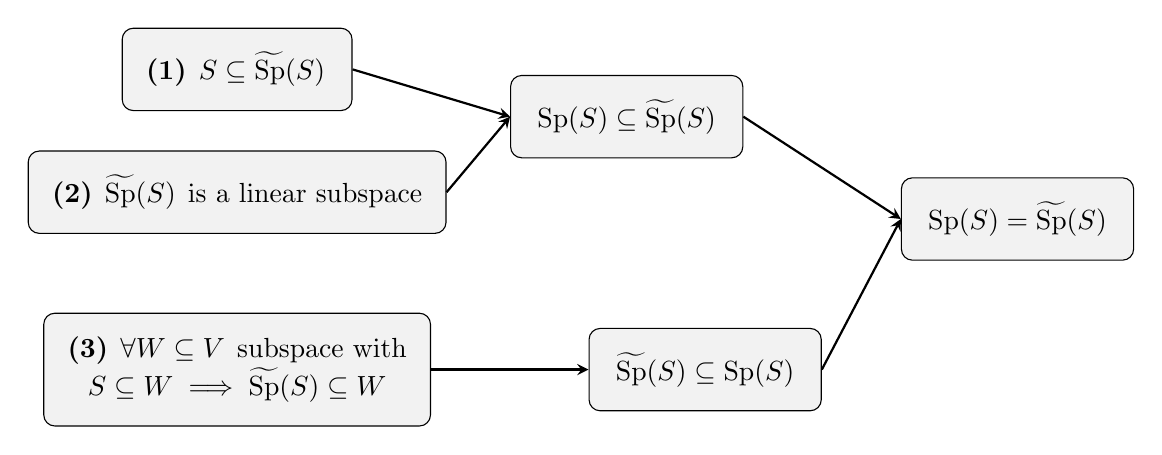
\begin{tikzpicture}[
    node distance=1.5cm and 2cm,
    box/.style={draw, rounded corners, fill=gray!10, align=center, inner sep=2ex},
    arrow/.style={->, thick, >=stealth}
]
    % Left Column (The 3 Facts)
    \node[box] (n1) {\textbf{(1)} $S \subseteq \widetilde{\Sp}(S)$};
    \node[box, below=0.5cm of n1] (n2) {\textbf{(2)} $\widetilde{\Sp}(S)$ is a linear subspace};
    \node[box, below=1cm of n2] (n3) {\textbf{(3)} $\forall W \subseteq V$ subspace with \\ $S \subseteq W \implies \widetilde{\Sp}(S) \subseteq W$};
    
    % Middle Column (Implications)
    \node[box, right=2cm of n1, yshift=-0.6cm] (p1) {$\Sp(S) \subseteq \widetilde{\Sp}(S)$};
    \node[box, right=2cm of n3] (p2) {$\widetilde{\Sp}(S) \subseteq \Sp(S)$};
    
    % Right Column (Conclusion)
    \node[box, right=2cm of p1, yshift=-1.3cm] (final) {$\Sp(S) = \widetilde{\Sp}(S)$};
    
    % Arrows mapping the logic
    \draw[arrow] (n1.east) -- (p1.west);
    \draw[arrow] (n2.east) -- (p1.west);
    \draw[arrow] (n3.east) -- (p2.west);
    
    \draw[arrow] (p1.east) -- (final.west);
    \draw[arrow] (p2.east) -- (final.west);
\end{tikzpicture}
\end{center}

Note that (1) and (2) imply that $\Sp(S) \subseteq \widetilde{\Sp}(S)$ because $\Sp(S)$ is defined as the intersection of \textit{all} subspaces containing $S$. Furthermore, (3) implies that $\widetilde{\Sp}(S) \subseteq \Sp(S)$ because $\Sp(S)$ is itself a valid subspace $W$ containing $S$.

\textbf{Proof of (1):} Let $v \in S$. Then we can write $v = 1 \cdot v \in \widetilde{\Sp}(S)$. Thus $S \subseteq \widetilde{\Sp}(S)$.

\textbf{Proof of (2):} 
First, $0_V \in \widetilde{\Sp}(S)$ because for any $w \in S$, $0 \cdot w = 0_V$. 
Second, let $u, v \in \widetilde{\Sp}(S)$. Then $u = a_1 w_1 + \dots + a_n w_n$ and $v = b_1 v_1 + \dots + b_m v_m$. Their sum:
\[
u + v = a_1 w_1 + \dots + a_n w_n + b_1 v_1 + \dots + b_m v_m \in \widetilde{\Sp}(S)
\]
Third, let $c \in K$ and $u \in \widetilde{\Sp}(S)$. Then:
\[
c \cdot u = c(a_1 w_1 + \dots + a_n w_n) = (c a_1)w_1 + \dots + (c a_n)w_n \in \widetilde{\Sp}(S)
\]
Thus $\widetilde{\Sp}(S)$ is closed under addition and scalar multiplication, making it a subspace.

\textbf{Proof of (3):} Let $W \subseteq V$ be an arbitrary subspace such that $S \subseteq W$. Let $u \in \widetilde{\Sp}(S)$. Then $u = a_1 w_1 + \dots + a_n w_n$ with elements $w_i \in S$. Since $S \subseteq W$, we know $w_i \in W$. Since $W$ is a subspace, it is closed under scalar multiplication and finite addition, which guarantees $a_1 w_1 + \dots + a_n w_n \in W$. So $u \in W$. Thus $\widetilde{\Sp}(S) \subseteq W$.
\end{proof}

\subsection{Checking for Span: The Bridge to Computations}

Up to this point, our definition of the span has been highly abstract. We know that if $S = \{w_1, \dots, w_n\}$ is a finite set, we can drop the set brackets and write its span as the set of all possible linear combinations:
\[
\Sp(w_1, \dots, w_n) = \{x_1 w_1 + \dots + x_n w_n \mid x_1, \dots, x_n \in K\}
\]
However, as a student of linear algebra, you should immediately ask a practical, computational question: \textbf{If I hand you a specific, concrete target vector $w$, how can we mathematically determine whether or not $w \in \Sp(w_1, \dots, w_n)$?}

To build our intuition, let us translate this abstract geometric question into algebra. Suppose our vector space is $V = K^m$. This means our vectors are just column vectors with $m$ entries. 

If $w$ is indeed in the span of $w_1, \dots, w_n$, there must exist some scalar "weights" $x_1, \dots, x_n \in K$ that allow us to build $w$. In other words, we need to solve the vector equation:
\begin{equation} \label{eq:vector_combo}
x_1 w_1 + x_2 w_2 + \dots + x_n w_n = w
\end{equation}

Let us write these vectors out explicitly by their components:
\[
w_1 = \begin{pmatrix} w_{1,1} \\ w_{2,1} \\ \vdots \\ w_{m,1} \end{pmatrix}, \quad w_2 = \begin{pmatrix} w_{1,2} \\ w_{2,2} \\ \vdots \\ w_{m,2} \end{pmatrix}, \quad \dots \quad , \quad w_n = \begin{pmatrix} w_{1,n} \\ w_{2,n} \\ \vdots \\ w_{m,n} \end{pmatrix}, \quad \text{and target } w = \begin{pmatrix} w_1 \\ w_2 \\ \vdots \\ w_m \end{pmatrix}
\]

If we substitute these columns into Equation \eqref{eq:vector_combo} and perform the scalar multiplication and vector addition component by component, we get a massive single column vector on the left side:
\[
\begin{pmatrix} 
x_1 w_{1,1} + x_2 w_{1,2} + \dots + x_n w_{1,n} \\ 
x_1 w_{2,1} + x_2 w_{2,2} + \dots + x_n w_{2,n} \\ 
\vdots \\ 
x_1 w_{m,1} + x_2 w_{m,2} + \dots + x_n w_{m,n} 
\end{pmatrix} 
= 
\begin{pmatrix} w_1 \\ w_2 \\ \vdots \\ w_m \end{pmatrix}
\]

Look closely at the left-hand side. This is exactly the definition of matrix-vector multiplication! We can seamlessly separate the known vector components from the unknown scalar weights $x_i$ by factoring this out into a coefficient matrix $A$ multiplied by a variable vector $x$:
\[
\underbrace{\begin{pmatrix} 
w_{1,1} & w_{1,2} & \dots & w_{1,n} \\ 
w_{2,1} & w_{2,2} & \dots & w_{2,n} \\ 
\vdots & \vdots & \ddots & \vdots \\ 
w_{m,1} & w_{m,2} & \dots & w_{m,n} 
\end{pmatrix}}_{\text{Matrix } A \text{ (whose columns are } w_i)}
\underbrace{\begin{pmatrix} x_1 \\ x_2 \\ \vdots \\ x_n \end{pmatrix}}_{\text{Vector } x}
= 
\underbrace{\begin{pmatrix} w_1 \\ w_2 \\ \vdots \\ w_m \end{pmatrix}}_{\text{Target } w}
\]

This reveals one of the most profound and useful insights in all of linear algebra: \textbf{A matrix-vector product $A \cdot x$ is simply a linear combination of the columns of $A$, weighted by the entries of $x$.} 

\begin{theorem}
Let $w, w_1, \dots, w_n \in K^m$. Let $A \in \M_{m \times n}(K)$ be the matrix whose columns are exactly the vectors $w_1, \dots, w_n$. Then the target vector $w$ is in the span of $w_1, \dots, w_n$ if and only if the system of linear equations $A \cdot x = w$ has at least one solution $x = (x_1, \dots, x_n)^T \in K^n$. 
\[
w \in \Sp(w_1, \dots, w_n) \iff \text{The system } A \cdot x = w \text{ is consistent.}
\]
\end{theorem}

\begin{remark}[How to check this in practice]
Because of this beautiful equivalence, whenever you are asked "Is $w$ in the span of these vectors?", you do not need to guess the coefficients. You simply construct the augmented matrix $(A \mid w)$ and perform Gaussian elimination. If the resulting system yields a contradiction, the vector is \textbf{not} in the span. If the system is solvable, the solutions $x_1, \dots, x_n$ are exactly the coefficients you need to build $w$.
\end{remark}

\subsection{Some spaces and how to generate them}

To conclude, let us look at some standard vector spaces and identify natural sets of "building block" vectors that span them entirely.

\begin{enumerate}
    \item \textbf{The Coordinate Space $K^n$:} 
    Let $e_1 = (1, 0, \dots, 0)$, $e_2 = (0, 1, 0, \dots, 0)$, $\dots$, $e_n = (0, \dots, 0, 1)$ be the standard basis vectors. Every vector $(x_1, \dots, x_n)$ can trivially be written as $x_1 e_1 + \dots + x_n e_n$.
    Then $K^n = \Sp(e_1, \dots, e_n)$. (\textbf{check!})
    
    \item \textbf{Bounded Polynomials $K[x]_d$:} 
    Let $W = K[x]_d$ be the space of polynomials over $K$ of degree $\le d$. 
    We can generate this space using the standard monomials:
    \[
    W = \Sp(1, x, x^2, \dots, x^d)
    \]
    
    \item \textbf{All Polynomials $K[x]$:} 
    Let $V = K[x]$ be the space of \textit{all} polynomials over $K$. 
    Generating this space requires an infinite set, as there is no maximum degree limit:
    \[
    V = \Sp(\{1, x, x^2, \dots, x^n, \dots\})
    \]
    
    \item \textbf{Spaces of Matrices $\M_{m \times n}(K)$:} 
    Consider the vector space of all $m \times n$ matrices over $K$. We can generate this entire space using the \textit{standard matrix basis}. 
    Let $E_{i,j}$ be the $m \times n$ matrix that has a $1$ in the $i$-th row and $j$-th column, and $0$ everywhere else. There are exactly $m \cdot n$ such matrices.
    
    For any arbitrary matrix $A = (A_{i,j}) \in \M_{m \times n}(K)$, we can pull it apart into a linear combination where the scalar weights are simply the matrix entries themselves:
    \[
    A = \sum_{i=1}^m \sum_{j=1}^n A_{i,j} \cdot E_{i,j}
    \]
    For instance, in $\M_{2 \times 2}(K)$, any matrix can be constructed like this:
    \[
    \begin{pmatrix} a & b \\ c & d \end{pmatrix} = a \begin{pmatrix} 1 & 0 \\ 0 & 0 \end{pmatrix} + b \begin{pmatrix} 0 & 1 \\ 0 & 0 \end{pmatrix} + c \begin{pmatrix} 0 & 0 \\ 1 & 0 \end{pmatrix} + d \begin{pmatrix} 0 & 0 \\ 0 & 1 \end{pmatrix}
    \]
    Thus, a matrix can be viewed as a "vector" built out of simpler matrices! We write:
    \[
    \M_{m \times n}(K) = \Sp(\{E_{i,j} \mid 1 \le i \le m, 1 \le j \le n\})
    \]
    (\textbf{check!!})
\end{enumerate}
\input{content/linear-independence.tex}
\input{content/bases-part-a.tex}
\input{content/bases-part-b.tex}
\setcounter{chapter}{11} % Sets chapter counter so the current chapter is 12
\renewcommand{\thetheorem}{\thechapter.\arabic{theorem}}
\setcounter{theorem}{0}

\chapter{Dimension and Subspaces}
In this chapter, we synthesize the fundamental results regarding finite-di\-men\-sional vector spaces and explore the relationship between a space and its subspaces through the lens of dimensionality.

\begin{summary}[Properties of Finite-Dimensional Spaces]
Let $V$ be a finite-di\-men\-sional vector space over a field $K$. The following structural principles hold:
\begin{enumerate}
    \item Every finite list of vectors that spans $V$ contains a sublist which constitutes a \qt{basis} of $V$. Formally, if $(v_1, \dots, v_n)$ spans $V$, then there exists a sublist $(v_{i_1}, \dots, v_{i_d})$ with $1 \le i_1 < i_2 < \dots < i_d \le n$ that is a basis for $V$, where $d = \dim V$.
    \item Every linearly independent list of vectors in $V$ can be extended to a basis of $V$. If the list $(u_1, \dots, u_m)$ is linearly independent, there exist vectors $w_1, \dots, w_{d-m}$ such that 
    \[(u_1, \dots, u_m, w_1, \dots, w_{d-m})\] 
    is a basis of $V$, where $d = \dim V$.
\end{enumerate}
\end{summary}

% thm:12.1
\begin{theorem}[Equivalent Characterizations of a Basis]
\label{thm:basis_equivalent_characterizations}
Let $V$ be a vector space with $\dim V = n \in \mathbb{Z}_{\ge 0}$. Let $v_1, \dots, v_n \in V$ be a list of $n$ vectors. Then the following statements are equivalent:
\begin{enumerate}
    \item[\textbf{(a)}] The vectors $v_1, \dots, v_n$ are linearly independent.
    \item[\textbf{(b)}] The vectors $v_1, \dots, v_n$ generate $V$, i.e., $\Sp(v_1, \dots, v_n) = V$.
    \item[\textbf{(c)}] The vectors $v_1, \dots, v_n$ constitute a basis for $V$.
\end{enumerate}
\end{theorem}

\begin{proof}
The equivalence is established through the following implications:

\textbf{(a) $\implies$ (c):} Suppose that \textbf{(a)} holds, so the list $v_1, \dots, v_n$ is linearly independent. According to the property that every linearly independent list can be extended to a basis, and observing that the list already possesses length $n = \dim V$, the extension requires no additional vectors. Thus, the list is already a basis for $V$, satisfying \textbf{(c)}.

\textbf{(c) $\implies$ (a) \& (b):} This follows directly from the definition of a basis, which by requirement must satisfy both the condition of linear independence in \textbf{(a)} and the spanning property in \textbf{(b)}.

\textbf{(b) $\implies$ (c):} If the spanning property in \textbf{(b)} holds, the list $v_1, \dots, v_n$ generates $V$. By the properties of finite-dimensional spaces, this list must contain a sublist that is a basis. Since $\dim V = n$, any basis must have exactly length $n$. Therefore, the sublist must be the entire list itself, making $v_1, \dots, v_n$ a basis as required by \textbf{(c)}.
\end{proof}



% prop:12.2
\begin{proposition}[Dimensional Constraints on Subspaces]
\label{prop:subspace_dimension_constraints}
Let $V$ be a finite-di\-men\-sional vector space over $K$. Then every linear subspace $U \subseteq V$ is also finite-di\-men\-sional. Moreover, $\dim U \le \dim V$, with the equality $\dim U = \dim V$ holding if and only if $U = V$.
\end{proposition}

\begin{proof}
Let $n = \dim V$. We first establish that $U$ possesses a finite basis. If $U = \{0\}$, the empty set serves as the basis and we are done. Assume $U \neq \{0\}$. We select a non-zero vector $v_1 \in U$. If $\Sp(v_1) = U$, we have found our basis. 

If $\Sp(v_1) \neq U$, we choose a second vector $v_2 \in U \setminus \Sp(v_1)$. It follows from the properties of linear independence that the list $\{v_1, v_2\}$ is linearly independent. We proceed iteratively: after $j$ steps, we obtain a linearly independent list $\{v_1, \dots, v_j\} \subseteq U$. If $\Sp(v_1, \dots, v_j) = U$, the process terminates. Otherwise, we choose $v_{j+1} \in U \setminus \Sp(v_1, \dots, v_j)$. By the principle that adding a vector outside the span of a linearly independent set preserves independence, the expanded list $\{v_1, \dots, v_{j+1}\}$ remains linearly independent.

Crucially, in a space $V$ of dimension $n$, no linearly independent list can exceed length $n$. Consequently, this algorithmic procedure must terminate in $k$ steps, where $k \le n$. At this stage, we have a list $\{v_1, \dots, v_k\}$ that is linearly independent and spans $U$, thereby constituting a basis for $U$. This implies $U$ is finite-dimensional and $\dim U = k \le n = \dim V$.

Furthermore, if $\dim U = \dim V = n$, then $U$ contains a linearly independent list of length $n$. By Theorem \ref{thm:basis_equivalent_characterizations}, such a list satisfies property \textbf{(a)} and is therefore also a basis for $V$. This implies $\Sp(v_1, \dots, v_n) = V$. Since $U = \Sp(v_1, \dots, v_n)$ by the construction of the basis, we conclude $U = V$.
\end{proof}
\setcounter{chapter}{12} % Sets chapter counter so the current chapter is 13
\renewcommand{\thetheorem}{\thechapter.\arabic{theorem}}
\setcounter{theorem}{0}

\chapter{Row and Column Spaces}

In this chapter, we bridge the abstract theory of vector spaces with the algorithmic power of matrix theory. We use Gauss elimination as a scalpel to dissect the structure of coordinate spaces.

\subsection{Linear Combinations and Matrix Equations}

Consider the vector space $K^{m}$ over a field $K$. Let $w_{1}, \dots, w_{n} \in K^{m}$ be a collection of vectors. We begin by addressing three fundamental questions that govern our understanding of these spaces.

\begin{question}[The Three Fundamental Questions]
\label{q:foundational_questions}
\begin{enumerate}
    \item How can we systematically determine if a given vector $w \in K^{m}$ belongs to the span $\Sp(w_{1}, \dots, w_{n})$?
    \item Can we describe the subspace $\Sp(w_{1}, \dots, w_{n})$ precisely using algebraic conditions?
    \item How can we determine whether the vectors $w_{1}, \dots, w_{n}$ are linearly independent?
\end{enumerate}
\end{question}

\begin{answer}[To Questions 1 and 2]
By definition, $w \in \Sp(w_{1}, \dots, w_{n})$ if and only if there exist scalars $x_{1}, \dots, x_{n} \in K$ such that $w = x_{1} w_{1} + \dots + x_{n} w_{n}$. We can assemble the vectors $w_{j}$ as columns of an $m \times n$ matrix $A$. This abstract linear combination is equivalent to the matrix equation:
\[
\underbrace{\begin{pmatrix} | & & | \\ w_{1} & \dots & w_{n} \\ | & & | \end{pmatrix}}_{A} \cdot \begin{pmatrix} x_{1} \\ \vdots \\ x_{n} \end{pmatrix} = \begin{pmatrix} | \\ w \\ | \end{pmatrix}
\]
Thus, $w$ is in the span if and only if the linear system $Ax = w$ is \qt{consistent} (i.e., it possesses at least one valid solution vector $x$). We analyze this by applying Gauss elimination on the augmented matrix $(A \mid w)$. 

To answer the second question and describe the entire span precisely, we replace the specific target $w$ with a general, variable vector $b = (b_{1}, \dots, b_{m})^{T}$ and reduce the augmented matrix $(A \mid b)$ to a row-reduced echelon form $(A' \mid b')$. 

This row operation procedure transforms our original problem into a much simpler, equivalent linear system $A'x = b'$. As shown in Prof. Biran's notes, the resulting matrix generally has the following characteristic block structure:
\begin{equation}
\label{eq:block_consistency}
(A' \mid b') = \left( 
\begin{array}{ccc|c}
* & \dots & * & b'_{1} \\
\vdots & \text{\footnotesize Rows with pivots} & \vdots & \vdots \\
* & \dots & * & b'_{r} \\ \hline
0 & \dots & 0 & b'_{r+1} \\
\vdots & \text{\footnotesize Zero rows} & \vdots & \vdots \\
0 & \dots & 0 & b'_{m}
\end{array} 
\right)
\end{equation}
In this reduced block structure, any row of $A'$ consisting entirely of zeros translates to an algebraic equation of the form $0 = b'_{i}$. For the overall system to be consistent (meaning a solution actually exists), it is an absolute requirement that the right-hand side of these specific equations also evaluates to zero. 

In other words, the system is consistent if and only if the entries in $b'$ corresponding to the zero-rows of $A'$ strictly vanish. Therefore, we can concisely describe the span as the set of all vectors satisfying these constraints:
\[
\Sp(w_{1}, \dots, w_{n}) = \left\{ b \in K^{m} \;\middle|\; b'_{r+1} = \dots = b'_{m} = 0 \right\}.
\]
\end{answer}

% ex:13.1
\begin{example}[Calculating a Specific Span]
\label{ex:span_calc}
Let $v_{1} = (1, 1, 1)^{T}$ and $v_{2} = (1, 0, -1)^{T} \in K^{3}$. To describe $\Sp(v_{1}, v_{2})$, we set up the augmented matrix with a general vector $b$ and row-reduce:
\[
\left( \begin{array}{cc|c} 1 & 1 & b_{1} \\ 1 & 0 & b_{2} \\ 1 & -1 & b_{3} \end{array} \right) \xrightarrow{R_{2}-R_{1}, R_{3}-R_{1}} \left( \begin{array}{cc|c} 1 & 1 & b_{1} \\ 0 & -1 & b_{2}-b_{1} \\ 0 & -2 & b_{3}-b_{1} \end{array} \right) \xrightarrow{R_{3}-2R_{2}} \left( \begin{array}{cc|c} 1 & 1 & b_{1} \\ 0 & -1 & b_{2}-b_{1} \\ \hline 0 & 0 & b_{1}-2b_{2}+b_{3} \end{array} \right)
\]
The system is consistent if and only if the expression corresponding to the zero-row evaluates to zero. Thus, the span is perfectly described by that single plane equation:
\[
\Sp(v_{1}, v_{2}) = \{ (b_{1}, b_{2}, b_{3})^{T} \in K^{3} \mid b_{1} - 2b_{2} + b_{3} = 0 \}.
\]
\end{example}

\begin{answer}[To Question 3]
The vectors are linearly independent if and only if the homogeneous equation $Ax = 0$ has only the trivial solution (i.e., $x_1 = \dots = x_n = 0$). 

This occurs if and only if the row-reduced echelon form $A'$ has a pivot in every column. If even a single column lacks a pivot, the corresponding variable becomes \qt{free} (e.g., it can be parameterized to take on any scalar value). The existence of a free variable immediately allows for non-trivial solutions, which by definition means the vectors are linearly dependent.
\end{answer}

% thm:13.2
\begin{theorem}[Fundamental Constraints on Coordinate Vectors]
\label{thm:coordinate_constraints}
Let $v_{1}, \dots, v_{n} \in K^{m}$.
\begin{enumerate}
    \item If $n > m$, then the vectors $v_{1}, \dots, v_{n}$ are linearly dependent.
    \item If $n < m$, then the vectors $v_{1}, \dots, v_{n}$ cannot span $K^{m}$.
\end{enumerate}
\end{theorem}

\begin{proof}
\begin{enumerate}
    \item Let $A = (v_{1} \mid \dots \mid v_{n})$. The number of pivots in $A'$ is bounded by the number of rows $m$. If $n > m$, at least $n - m$ columns are forced to be without pivots. These free variables guarantee non-trivial solutions to $Ax = 0$, hence dependence.
    \item The number of pivots is bounded by the number of columns $n$. If $n < m$, there are at least $m - n$ zero-rows in $A'$. By the logic of equation \eqref{eq:block_consistency}, we can easily choose a vector $b$ such that the resulting $b'$ has non-zero entries in those bottom rows, making the system inconsistent.
\end{enumerate}
\end{proof}

\subsection{Row and Column Spaces}

% def:13.4
\begin{definition}[Subspaces of a Matrix]
\label{def:matrix_subspaces}
Let $A \in \M_{m \times n}(K)$.
\begin{enumerate}
\item The \qt{column space} $\ColS(A) \subseteq K^{m}$ is the span of the columns of $A$.
\item The \qt{row space} $\RowS(A) \subseteq K^{n}$ is the span of the rows of $A$.
\end{enumerate}
\end{definition}

% prop:13.5
\begin{proposition}[Invariance of Row Space]
\label{prop:row_space_invariance}
Elementary row operations do not change the row space: $\RowS(A) = \RowS(A')$.
\end{proposition}

\begin{proof}
New rows are, simply, linear combinations of the old rows, and because elementary operations are reversible, the spans remain identical.
\end{proof}

\begin{importantremark}
Row operations \textbf{do} change the column space, as seen by $\begin{pmatrix} 1 & 1 \\ 1 & 1 \end{pmatrix} \to \begin{pmatrix} 1 & 1 \\ 0 & 0 \end{pmatrix}$. However, they \textbf{preserve} the linear relations between columns: $\sum \alpha_{i} w_{i} = 0 \iff \sum \alpha_{i} w'_{i} = 0$.
\end{importantremark}

\subsection{Constructing Bases}

% thm:13.7
\begin{theorem}[Basis for the Column Space]
\label{thm:basis_col_space}
The columns of $A$ that correspond to the \qt{pivot columns} of its row-reduced echelon form $B$ constitute a basis for $\ColS(A)$.
\end{theorem}

\begin{proof}
By the principle that row operations preserve the linear dependence relations between columns, we have:
\[
\sum_{i=1}^n \alpha_i w_i = 0 \iff \sum_{i=1}^n \alpha_i w'_i = 0.
\]
Thus, a set of columns in $A$ is linearly independent (or spans the column space) if and only if the corresponding set of columns in $B$ possesses the same property in $\ColS(B)$.

Consider the row-reduced echelon matrix $B \in \M_{m \times n}(K)$ with $r$ pivots. We visualize its block structure and the specific indices of its pivot columns $j_1, j_2, \dots, j_r$:

\begin{equation}
\label{eq:matrix_B_rigorous}
B = \left( 
\begin{array}{ccccccccc}
 & \text{\tiny col } j_1 & & \text{\tiny col } j_2 & & \text{\tiny col } j_r & & & \\
 & \downarrow & & \downarrow & & \downarrow & & & \\
\dots & \mathbf{1} & * & \mathbf{0} & * & \mathbf{0} & * & \dots & \leftarrow 1 \\
\dots & \mathbf{0} & \dots & \mathbf{1} & \dots & \mathbf{0} & * & \dots & \leftarrow 2 \\
 & \vdots & & \vdots & \ddots & \vdots & \vdots & & \vdots \\
\dots & \mathbf{0} & \dots & \mathbf{0} & \dots & \mathbf{1} & * & \dots & \leftarrow r \\ \hline
 & 0 & & 0 & & 0 & 0 & \dots & \\
 & \vdots & & \vdots & & \vdots & \vdots & \ddots & \\
 & 0 & & 0 & & 0 & 0 & \dots & 
\end{array} 
\right)
\end{equation}

In this echelon form, the pivot columns are precisely the first $r$ standard basis vectors of $K^m$:
\[
e_1 = \begin{pmatrix} 1 \\ 0 \\ \vdots \\ 0 \\ \vdots \\ 0 \end{pmatrix}, \quad 
e_2 = \begin{pmatrix} 0 \\ 1 \\ \vdots \\ 0 \\ \vdots \\ 0 \end{pmatrix}, \quad \dots, \quad 
e_r = \begin{pmatrix} 0 \\ \vdots \\ 1 \\ 0 \\ \vdots \\ 0 \end{pmatrix}
\]
where for each $e_i$, the entry $1$ is located at the $i$-th row. Because $B$ is in row-reduced echelon form, every entry in every column $w'_j$ that lies below the $r$-th row must be zero. This implies that:
\[
w'_j \in K^r \times \{0\}^{m-r} = \left\{ (x_1, \dots, x_r, 0, \dots, 0)^{T} \in K^m \right\}.
\]
Since the standard basis vectors $e_1, \dots, e_r$ are clearly linearly independent and they span the subspace $K^r \times \{0\}^{m-r}$, we establish the following chain of inclusions:
\[
K^r \times \{0\}^{m-r} = \Sp(e_1, \dots, e_r) \subseteq \ColS(B) \subseteq K^r \times \{0\}^{m-r}.
\]
This double inclusion forces the equality $\ColS(B) = \Sp(e_1, \dots, e_r) = K^r \times \{0\}^{m-r}$. Consequently, the pivot columns of $B$ form a basis for its column space. By the preservation of linear relations, the corresponding columns in the original matrix $A$ form a basis for $\ColS(A)$.
\end{proof}

% thm:13.8
\begin{theorem}[Basis for the Row Space]
\label{thm:row_basis}
The non-zero rows of the row-reduced echelon matrix $B$ form a basis for $\RowS(A)$.
\end{theorem}

\begin{corollary}[Rank Invariance]
\label{cor:rank_invariance}
The number of pivots is independent of the sequence of row operations, as it always equals $\dim \RowS(A)$.
\end{corollary}

% thm:13.13
\begin{theorem}[The Rank Equality]
\label{thm:rank_equality}
For any $A \in \M_{m \times n}(K)$, $\dim \RowS(A) = \dim \ColS(A)$. This shared dimension is the \qt{rank} of $A$, denoted $\rank(A)$.
\end{theorem}

\begin{proof}
Let $r$ be the number of pivots in the RREF of $A$. By Theorem \ref{thm:basis_col_space}, $\dim \ColS(A) = r$. By Theorem \ref{thm:row_basis}, $\dim \RowS(A) = r$. Thus, the dimensions are exactly equal.
\end{proof}
% Overriding the theorem counter for this chapter to match the 14.1, 14.2 convention
\renewcommand{\thetheorem}{\thechapter.\arabic{theorem}}
\setcounter{chapter}{13} % Sets chapter counter so the current chapter is 14
\setcounter{theorem}{0}

\chapter{Sums of Vector Spaces}

% def:14.1
\begin{definition}[Sum of Subspaces]
\label{def:sum_of_subspaces}
Let $V$ be a vector space over $K$, and let $U, W \subseteq V$ be linear subspaces. We define the \qt{sum} of $U$ and $W$, denoted by $U + W$, as the set:
\[
U + W := \{u + w \mid u \in U, w \in W\}.
\]
In a similar way, we can define sums of more than two subspaces. If $U_1, \dots, U_r \subseteq V$ are subspaces, we define their total sum as:
\[
U_1 + \dots + U_r := \{u_1 + \dots + u_r \mid u_1 \in U_1, \dots, u_r \in U_r\}.
\]
\end{definition}

% prop:14.2
\begin{proposition}[Properties of Sums]
\label{prop:properties_of_sums}
Let $U, W \subseteq V$ be subspaces. Then, the following properties hold:
\begin{enumerate}
    \item $U + W = \operatorname{Sp}(U \cup W)$. In particular, $U + W \subseteq V$ is a subspace, and $U$ and $W$ are themselves subspaces of $U + W$.
    \item If $U$ and $W$ are finite-dimensional, then so is $U + W$. Moreover, one can systematically find a basis for $U + W$ by following these sequential steps: first, choose a basis $(v_1, \dots, v_k)$ for $U \cap W$ (where $k = \dim(U \cap W)$). Second, extend this to a basis $(v_1, \dots, v_k, u_1, \dots, u_{l-k})$ for $U$ (where $l = \dim U$). Third, extend the initial intersection basis to a basis $(v_1, \dots, v_k, w_1, \dots, w_{m-k})$ for $W$ (where $m = \dim W$). Finally, the combined elements 
    \[(v_1, \dots, v_k, u_1, \dots, u_{\ell-k}, w_1, \dots, w_{m-k})\] 
    form a basis for $U + W$.
\end{enumerate}
\end{proposition}

\begin{proof}
We will explicitly prove the second statement. By definition, the subspace $U + W$ is generated by the combined vectors $(v_1, \dots, v_k, u_1, \dots, u_{l-k}, w_1, \dots, w_{m-k})$. It remains to show that these vectors are linearly independent.

Suppose there exists a linear combination equal to the zero vector:
\begin{equation}
\label{eq:linear_comb_sum}
\alpha_1 v_1 + \dots + \alpha_k v_k + \beta_1 u_1 + \dots + \beta_{\ell-k} u_{\ell-k} + \gamma_1 w_1 + \dots + \gamma_{m-k} w_{m-k} = 0.
\end{equation}
We can rearrange this equation to isolate the terms belonging to $U$ and $W$:
\[
\underbrace{\beta_1 u_1 + \dots + \beta_{\ell-k} u_{\ell-k}}_{\in U} = \underbrace{-\alpha_1 v_1 - \dots - \alpha_k v_k - \gamma_1 w_1 - \dots - \gamma_{m-k} w_{m-k}}_{\in W}.
\]
Let us denote this common vector by $x$. Since the left side is entirely in $U$ and the right side is entirely in $W$, we have $x \in U$ and $x \in W$, which implies $x \in U \cap W$. 

Because $(v_1, \dots, v_k)$ is a basis for $U \cap W$, there must exist scalars $\delta_1, \dots, \delta_k \in K$ such that:
\[
x = \delta_1 v_1 + \dots + \delta_k v_k.
\]
Equating this with our original expression for $x$ in $U$, we obtain:
\[
\beta_1 u_1 + \dots + \beta_{\ell-k} u_{\ell-k} = \delta_1 v_1 + \dots + \delta_k v_k \implies \sum_{i=1}^{\ell-k} \beta_i u_i - \sum_{j=1}^k \delta_j v_j = 0.
\]
However, the vectors $(v_1, \dots, v_k, u_1, \dots, u_{\ell-k})$ form a basis for $U$, meaning they are strictly linearly independent. Consequently, all coefficients in this sum must be zero. In particular, $\beta_1 = \dots = \beta_{\ell-k} = 0$.

Substituting these zero values back into our initial equation \eqref{eq:linear_comb_sum}, the terms involving $u_i$ vanish, leaving:
\[
\alpha_1 v_1 + \dots + \alpha_k v_k + \gamma_1 w_1 + \dots + \gamma_{m-k} w_{m-k} = 0.
\]
Since the vectors $(v_1, \dots, v_k, w_1, \dots, w_{m-k})$ form a basis for $W$, they are linearly independent. This immediately implies that $\alpha_1 = \dots = \alpha_k = 0$ and $\gamma_1 = \dots = \gamma_{m-k} = 0$. 

Because all coefficients $\alpha_i$, $\beta_j$, and $\gamma_k$ have been forced to zero, the combined family of vectors is linearly independent, and therefore constitutes a valid basis for $U + W$.
\end{proof}

% thm:14.3
\begin{theorem}[Dimension Formula for Sums]
\label{thm:dimension_formula_sums}
Let $V$ be a vector space, and let $U, W \subseteq V$ be finite-dimensional subspaces. Then, the following dimension formula holds:
\[
\dim(U + W) = \dim U + \dim W - \dim(U \cap W).
\]
\end{theorem}

\begin{proof}
Using the basis constructed in Proposition \ref{prop:properties_of_sums}, we can directly count the number of basis vectors for $U + W$:
\begin{align*}
\dim(U + W) &= k + (\ell - k) + (m - k) \\
&= \ell + m - k \\
&= \dim U + \dim W - \dim(U \cap W).
\end{align*}
\end{proof}

% cor:unnumbered
\begin{corollary}[Equivalent Conditions for Trivial Intersection]
\label{cor:trivial_intersection}
Let $V$ be a vector space, and let $U, W \subseteq V$ be subspaces. The following statements are equivalent:
\begin{enumerate}
    \item $U \cap W = \{0\}$.
    \item For every $v \in U + W$, there exist unique vectors $u \in U$ and $w \in W$ such that $v = u + w$.
    \item Every $x \in U \cap W$ can be uniquely written as $x = u + w$ with $u \in U$ and $w \in W$.
    \item The equality $0 = u + w$ with $u \in U$ and $w \in W$ implies that $u = 0$ and $w = 0$.
\end{enumerate}
\end{corollary}

\begin{proof}
We prove the main equivalences by showing the cycle of implications \textbf{(a)} $\implies$ \textbf{(b)} $\implies$ \textbf{(d)} $\implies$ \textbf{(a)}. (The equivalence of \textbf{(c)} follows naturally from the same uniqueness constraints).

\textbf{(a) $\implies$ (b):} Suppose that $v \in U + W$ can be written in two ways: $v = u + w = u' + w'$, where $u, u' \in U$ and $w, w' \in W$. Rearranging this equation yields $u - u' = w' - w$. The left side is in $U$ and the right side is in $W$, which means the vector $u - u'$ resides in the intersection $U \cap W$. Since we assume $U \cap W = \{0\}$, it follows that $u - u' = 0$ and $w' - w = 0$. Therefore, $u = u'$ and $w = w'$, proving uniqueness.

\textbf{(b) $\implies$ (d):} Consider the zero vector, which can obviously be written as $0 = 0_U + 0_W$. If we also have $0 = u + w$ for some $u \in U$ and $w \in W$, the assumed uniqueness in statement \textbf{(b)} immediately forces $u = 0$ and $w = 0$.

\textbf{(d) $\implies$ (a):} Let $x \in U \cap W$. We can express the zero vector as $0 = x + (-x)$. Since $x \in U \cap W$, we know $x \in U$ and $-x \in W$. If statement \textbf{(d)} holds, this equality strictly implies $x = 0$. Consequently, the only element in the intersection is the zero vector, so $U \cap W = \{0\}$.
\end{proof}

\setcounter{theorem}{3} % Resets the theorem counter so the next environment is labeled 14.4

% def:14.4
\begin{definition}[Complement of a Subspace]
\label{def:complement}
Let $V$ be a vector space over $K$, and let $U \subseteq V$ be a subspace. A subspace $W \subseteq V$ is called a \qt{complement} of $U$ if it satisfies the following two conditions:
\[
U + W = V \quad \text{and} \quad U \cap W = \{0\}.
\]
\end{definition}

\begin{remark}
Note that if $W$ is a complement of $U$, then $U$ and $W$ satisfy all of the five equivalent statements derived from Corollary \ref{cor:trivial_intersection}.
\end{remark}

% prop:14.5
\begin{proposition}[Existence of a Complement]
\label{prop:existence_complement}
Let $V$ be a finite-dimensional vector space, and let $U \subseteq V$ be a subspace. Then, there exists a subspace $W \subseteq V$ which is a complement to $U$.
\end{proposition}

\begin{proof}
Choose a basis $\mathcal{B}_U = (u_1, \dots, u_{\ell})$ for $U$, where $\ell = \dim U$. By the Steinitz Exchange Lemma, we can extend this to a full basis for $V$:
\[
\mathcal{B}_V = (u_1, \dots, u_{\ell}, w_1, \dots, w_m),
\]
where $\ell + m = \dim V$. We define $W := \operatorname{Sp}(w_1, \dots, w_m)$. 

We claim that $W$ is a valid complement of $U$. Indeed, since the combined basis spans the entirety of $V$, it is clear that $U + W = V$. To see that $U \cap W = \{0\}$, let $x \in U \cap W$. Because $x \in U$, we can write $x = \sum_{i=1}^l a_i u_i$. Because $x \in W$, we can also write $x = \sum_{j=1}^m b_j w_j$. Equating these expressions yields:
\[
\sum_{i=1}^{\ell} a_i u_i = \sum_{j=1}^m b_j w_j \implies \sum_{i=1}^{\ell} a_i u_i - \sum_{j=1}^m b_j w_j = 0.
\]
Since $\mathcal{B}_V$ is a basis for $V$, all of its constituent vectors are strictly linearly independent. This forces all scalar coefficients to be zero: $a_i = 0$ for all $i$ and $b_j = 0$ for all $j$. Thus, $x = 0$, proving that $U \cap W = \{0\}$.
\end{proof}
% Overriding the theorem counter for this chapter to match the 15.0.1, 15.0.2 convention
\renewcommand{\thetheorem}{\arabic{chapter}.\alph{section}.\arabic{theorem}}

\setcounter{chapter}{14} % Sets chapter counter so the current chapter is 15
\chapter{Linear Maps}

\section{Introduction to Linear Maps}

Linear maps, also known as linear transformations, are homomorphisms of vector spaces. They are the primary objects of study in linear algebra, as they preserve the underlying algebraic structure of vector spaces.

% def:15.a.1
\begin{definition}[Linear Map]
\label{def:linear_map}
Let $V$ and $W$ be vector spaces over a field $K$. A map $T: V \to W$ is called a \qt{linear map} if it satisfies the following two conditions:
\begin{enumerate}
    \item For all $v_1, v_2 \in V$, $T(v_1 + v_2) = T(v_1) + T(v_2)$.
    \item For all $\alpha \in K$ and $v \in V$, $T(\alpha \cdot v) = \alpha \cdot T(v)$.
\end{enumerate}
\end{definition}

\begin{remark}[Notation and Terminology]
\label{rem:linear_map_notation}
In many contexts, we omit the parentheses and write $Tv$ instead of $T(v)$. The conditions outlined in Definition \ref{def:linear_map} essentially state that $T: V \to W$ is a map that respects the operations defined on the vector spaces; specifically, the addition and scalar multiplication in $V$ are mapped perfectly to the corresponding operations in $W$.

We denote the set of all linear maps from $V$ to $W$ by $\Hom_K(V, W)$, or simply $\Hom(V, W)$. While some authors use alternative notations such as $\operatorname{Lin}(V, W)$ or $\hom_K(V, W)$, $\Hom_K(V, W)$ remains the standard academic convention.
\end{remark}

\begin{exercise}[Linearity Criterion]
\label{exer:linearity_criterion}
Prove that a map $T: V \to W$ is linear if and only if for all $\alpha_1, \alpha_2 \in K$ and $v_1, v_2 \in V$:
\[
T(\alpha_1 v_1 + \alpha_2 v_2) = \alpha_1 T(v_1) + \alpha_2 T(v_2).
\]
\end{exercise}

\begin{example}[Fundamental Examples of Linear Maps]
\label{ex:fundamental_linear_maps}
\begin{enumerate}
    \item The identity map $\id_V: V \to V$, defined by $\id_V(v) := v$ for all $v \in V$.
    \item The zero map $0: V \to W$, defined by $0(v) := 0_W$ for all $v \in V$. 
    
    Clearly, these initial examples are elementary, yet they serve as vital benchmarks.
    
    \item The derivative map $D: K[x] \to K[x]$. For any polynomial $p(x) = \sum_{k=0}^n a_k x^k$, we define its image as:
    \[
    D(p(x)) := \sum_{k=1}^n k a_k x^{k-1}.
    \]
    This map is linear, as the derivative of a linear combination of polynomials is simply the same linear combination of their derivatives.
    
    \item Consider the vector space $C([a, b])$ consisting of continuous functions $f: [a, b] \to \mathbb{R}$. The definite integral defines a linear map $T: C([a, b]) \to \mathbb{R}$, given by:
    \[
    T(f) := \int_a^b f(x) \, dx.
    \]
    
    \item The shift map $S: K^\infty \to K^\infty$, defined on infinite sequences as:
    \[
    S((a_1, a_2, a_3, \dots)) := (a_2, a_3, a_4, \dots).
    \]
\end{enumerate}
\end{example}

\begin{example}[Matrix Transformation]
\label{ex:matrix_transformation}
This is a central example in finite-dimensional linear algebra. Let $A \in \M_{m \times n}(K)$ be a matrix. We define a map $T_A: K^n \to K^m$ via matrix-vector multiplication:
\[
T_A \left(\begin{smallmatrix} x_1 \\ \vdots \\ x_n \end{smallmatrix}\right) := A \cdot \left(\begin{smallmatrix} x_1 \\ \vdots \\ x_n \end{smallmatrix}\right).
\]
Recall from matrix arithmetic that $A \cdot (\alpha \cdot x) = \alpha \cdot (A \cdot x)$ and $A \cdot (x + y) = A \cdot x + A \cdot y$. Consequently, $T_A$ is a linear map.
\end{example}

% prop:15.a.2
\begin{proposition}[Basic Properties of Linear Maps]
\label{prop:properties_linear_maps}
Let $V$ and $W$ be vector spaces over a field $K$, and let $T: V \to W$ be a linear map. Then, the following properties hold:
\begin{enumerate}
    \item For all $n \in \mathbb{N}$, $\alpha_1, \dots, \alpha_n \in K$, and $v_1, \dots, v_n \in V$, we have:
    \[
    T\left( \sum_{i=1}^n \alpha_i v_i \right) = \sum_{i=1}^n \alpha_i T(v_i).
    \]
    \item $T(0_V) = 0_W$.
\end{enumerate}
\end{proposition}

\begin{proof}
\begin{enumerate}
    \item The first statement follows directly from the definition of linearity \eqref{def:linear_map} by applying induction on the number of vectors $n$.
    \item To prove the second statement, we evaluate the image of the zero vector:
    \[
    0_W = T(0_V) - T(0_V) = T(0_V - 0_V) = T(0_V).
    \]
    Therefore, any linear map must map the zero vector of the domain directly to the zero vector of the codomain.
\end{enumerate}
\end{proof}

% thm:15.a.3
\begin{theorem}[Existence and Uniqueness of Linear Maps on a Basis]
\label{thm:existence_uniqueness_linear_map}
Let $V$ be a finite-dimensional vector space, and let $\mathcal{B} = (v_1, \dots, v_n)$ be a basis for $V$. Given any arbitrary sequence of vectors $w_1, \dots, w_n \in W$, there exists a unique linear map $T: V \to W$ such that:
\[
T(v_i) = w_i, \quad \forall \, 1 \le i \le n.
\]
\end{theorem}

\begin{proof}
\textbf{Existence:} Let $v \in V$ be an arbitrary vector. Since $\mathcal{B}$ is a basis, there exist unique scalars $a_1, \dots, a_n \in K$ such that $v = \sum_{i=1}^n a_i v_i$. We define the map $T$ by setting:
\begin{equation}
\label{eq:T_def_existence}
T(v) := \sum_{i=1}^n a_i w_i.
\end{equation}
Because the coordinates $a_i$ are uniquely determined for each $v$, the map $T$ is well-defined. By verifying the conditions of Definition \ref{def:linear_map}, it is straightforward to show that $T$ is linear. Furthermore, for each basis vector $v_j$, the only non-zero coordinate is $a_j = 1$, which naturally implies $T(v_j) = w_j$.

\textbf{Uniqueness:} Suppose there exists another linear map $S: V \to W$ such that $S(v_i) = w_i$ for all $1 \le i \le n$. For any $v = \sum_{i=1}^n a_i v_i \in V$, the linearity of $S$ dictates:
\[
S(v) = S\left( \sum_{i=1}^n a_i v_i \right) = \sum_{i=1}^n a_i S(v_i) = \sum_{i=1}^n a_i w_i = T(v).
\]
Since $S(v) = T(v)$ for all $v \in V$, the maps are functionally identical, establishing that $S = T$.
\end{proof}

\stepcounter{theorem}
% ex:15.a.4
\begin{example}[Important Example 15.a.4: Linear Maps on Coordinate Spaces]
\label{ex:linear_map_std_basis}
Consider the coordinate space $K^n$ equipped with the standard basis $\mathcal{E} = (e_1, \dots, e_n)$. Let $w_1, \dots, w_n \in K^m$ be any vectors. Theorem \ref{thm:existence_uniqueness_linear_map} guarantees a unique linear map $T: K^n \to K^m$ such that $T(e_i) = w_i$ for all $1 \le i \le n$.

\begin{question}
Can we provide an explicit matrix description for this map $T$?
\end{question}

\begin{answer}
Let $A \in \M_{m \times n}(K)$ be the matrix whose $j$-th column is precisely the vector $w_j$:
\[
A = 
\begin{pmatrix}
| & & | \\
w_1 & \dots & w_n \\
| & & |
\end{pmatrix}.
\]
The linear transformation $T_A: K^n \to K^m$ defined by $v \mapsto A \cdot v$ easily satisfies $T_A(e_j) = w_j$ for all $j$. Due to the absolute uniqueness property established in Theorem \ref{thm:existence_uniqueness_linear_map}, we immediately conclude that $T = T_A$.
\end{answer}
\end{example}

% lem:15.a.5
\begin{lemma}[Matrix Representation of Linear Maps]
\label{lem:all_linear_maps_are_matrices}
For every linear transformation $T: K^n \to K^m$, there exists a unique matrix $A \in \M_{m \times n}(K)$ such that $T = T_A$.
\end{lemma}

\begin{proof}
Let $w_i = T(e_i)$ for each $i \in \{1, \dots, n\}$. As demonstrated in the preceding example, the matrix $A$ formed by using these specific vectors as columns defines a linear map $T_A$ that perfectly agrees with $T$ on the standard basis $\mathcal{E}$. Because $\mathcal{E}$ is a basis for $K^n$, Theorem \ref{thm:existence_uniqueness_linear_map} strictly implies that $T$ and $T_A$ must be the exact same map.
\end{proof}
\section{Kernel, Image, and the Rank-Nullity Theorem}

In this section, we explore two fundamental subspaces associated with every linear map: the kernel and the image. These subspaces provide deep insight into the structure of the transformation and ultimately lead us to one of the most celebrated results in linear algebra, the Rank-Nullity Theorem.

% prop:15.b.1
\begin{proposition}[Kernel and Image]
\label{prop:kernel_image}
Let $V$ and $W$ be vector spaces over a field $K$, and let $T: V \to W$ be a linear map.
\begin{enumerate}
    \item The set $\ker(T) := \{v \in V \mid T(v) = 0_W\} \subseteq V$ is a linear subspace of $V$. It is called the \qt{kernel} of $T$.
    \item The set $\operatorname{Im}(T) := \{T(v) \mid v \in V\} \subseteq W$ is a linear subspace of $W$. It is called the \qt{image} of $T$.
\end{enumerate}
\end{proposition}

\begin{remark}[Set-Theoretic Perspective]
\label{rem:set_theoretic_notation}
Using standard notation from set theory, we can concisely write the kernel as the fiber over the zero vector, $\ker(T) = T^{-1}(\{0_W\})$, and the image as the range of the entire domain, $\operatorname{Im}(T) = T(V)$. (Note: The image is sometimes denoted as $\operatorname{Image}(T)$).
\end{remark}

\begin{proof}[Proof of Proposition \ref{prop:kernel_image}]
\begin{enumerate}
    \item To show that $\ker(T) \subseteq V$ is a subspace, let $a, b \in K$, and let $v_1, v_2 \in \ker(T)$. By the linearity of $T$, we have:
    \[
    T(a v_1 + b v_2) = a T(v_1) + b T(v_2) = a \cdot 0_W + b \cdot 0_W = 0_W.
    \]
    This implies that $a v_1 + b v_2 \in \ker(T)$. Furthermore, since $T(0_V) = 0_W$, the zero vector $0_V \in \ker(T)$. Thus, the kernel is a valid subspace.
    
    \item To show that $\operatorname{Im}(T) \subseteq W$ is a subspace, let $a, b \in K$, and let $w_1, w_2 \in \operatorname{Im}(T)$. By definition, there exist vectors $v_1, v_2 \in V$ such that $T(v_1) = w_1$ and $T(v_2) = w_2$. Therefore, we can write:
    \[
    a w_1 + b w_2 = a T(v_1) + b T(v_2) = T(a v_1 + b v_2).
    \]
    Since $a v_1 + b v_2 \in V$, it follows immediately that $a w_1 + b w_2 \in \operatorname{Im}(T)$. Moreover, since $T(0_V) = 0_W$, we have $0_W \in \operatorname{Im}(T)$. Thus, the image is a subspace.
\end{enumerate}
\end{proof}

% prop:15.b.2
\begin{proposition}[Injectivity and the Kernel]
\label{prop:injectivity_kernel}
A linear map $T: V \to W$ is injective if and only if $\ker(T) = \{0_V\}$.
\end{proposition}

\begin{proof}
First, suppose $T$ is injective. If $v \in \ker(T)$, then $T(v) = 0_W$. Since we also know that $T(0_V) = 0_W$, the injectivity of $T$ forces $v = 0_V$. Thus, $\ker(T) = \{0_V\}$.

Conversely, suppose that $\ker(T) = \{0_V\}$. Let $v_1, v_2 \in V$ such that $T(v_1) = T(v_2)$. By linearity, we obtain:
\[
T(v_1) - T(v_2) = 0_W \implies T(v_1 - v_2) = 0_W.
\]
This implies that $v_1 - v_2 \in \ker(T)$. By our assumption, the only element in the kernel is the zero vector, and therefore, $v_1 - v_2 = 0_V$, which yields $v_1 = v_2$. Consequently, $T$ is injective.
\end{proof}

% def:15.b.3
\begin{definition}[Rank of a Linear Map]
\label{def:rank_linear_map}
Let $T: \in \Hom(V, W)$ be a linear map such that $\dim \operatorname{Im}(T) < \infty$. We define the \qt{rank} of $T$ as the dimension of its image:
\[
\rank(T) := \dim \operatorname{Im}(T).
\]
\end{definition}

% thm:15.b.4
\begin{theorem}[Rank-Nullity Theorem]
\label{thm:rank_nullity}
Let $V$ be a finite-dimensional vector space, and let $T: V \to W$ be a linear map. Then, the following dimension formula holds:
\[
\dim V = \dim \ker(T) + \dim \operatorname{Im}(T).
\]
\end{theorem}

\begin{proof}
Let $k = \dim \ker(T)$ and $n = \dim V$. Let $(u_1, \dots, u_k)$ be a basis for $\ker(T)$. By the Steinitz Exchange Lemma, we can extend this linearly independent set to a full basis for $V$, denoted by $\mathcal{B} = (u_1, \dots, u_k, v_1, \dots, v_{n-k})$. We claim that the family $\mathcal{C} = (T(v_1), \dots, T(v_{n-k}))$ forms a basis for $\operatorname{Im}(T)$.

\begin{enumerate}
    \item \textbf{Spanning:} Let $w \in \operatorname{Im}(T)$. By definition, there exists some $v \in V$ such that $w = T(v)$. We can express $v$ uniquely as a linear combination of the basis vectors in $\mathcal{B}$:
    \[
    v = \sum_{i=1}^k a_i u_i + \sum_{j=1}^{n-k} b_j v_j.
    \]
    Applying the linear map $T$, and recalling that $T(u_i) = 0_W$ for all $i$, we find:
    \begin{align*}
    w &= T\left( \sum_{i=1}^k a_i u_i + \sum_{j=1}^{n-k} b_j v_j \right) \\
    &= \sum_{i=1}^k a_i T(u_i) + \sum_{j=1}^{n-k} b_j T(v_j) \\
    &= 0_W + \sum_{j=1}^{n-k} b_j T(v_j).
    \end{align*}
    Thus, the vectors in $\mathcal{C}$ span $\operatorname{Im}(T)$.
    
    \item \textbf{Linear Independence:} Suppose there exist scalars $b_j \in K$ such that:
    \[
    \sum_{j=1}^{n-k} b_j T(v_j) = 0_W.
    \]
    By the linearity of $T$, this is equivalent to $T\left( \sum_{j=1}^{n-k} b_j v_j \right) = 0_W$, which implies that the vector $\sum_{j=1}^{n-k} b_j v_j$ lies in $\ker(T)$. Because $(u_1, \dots, u_k)$ is a basis for the kernel, there must exist scalars $a_i \in K$ such that:
    \[
    \sum_{j=1}^{n-k} b_j v_j = \sum_{i=1}^k a_i u_i \implies \sum_{j=1}^{n-k} b_j v_j - \sum_{i=1}^k a_i u_i = 0_V.
    \]
    However, since $\mathcal{B}$ is a basis for $V$, all of its constituent vectors are linearly independent. This forces all coefficients to be zero, specifically $b_j = 0$ for all $1 \le j \le n-k$. 
\end{enumerate}

Therefore, $\mathcal{C}$ is linearly independent and spans the image, making it a basis for $\operatorname{Im}(T)$. Consequently, $\dim \operatorname{Im}(T) = n - k = \dim V - \dim \ker(T)$.
\end{proof}

% cor:15.b.5
\begin{corollary}[Equivalence of Injectivity and Surjectivity]
\label{cor:equal_dim_iso}
Let $V$ and $W$ be finite-dimensional vector spaces such that $\dim V = \dim W$. For any linear map $T: V \to W$, the following statements are equivalent:
\begin{enumerate}
    \item $T$ is injective.
    \item $T$ is surjective.
    \item $T$ is an isomorphism.
\end{enumerate}
\end{corollary}

\begin{proof}
By the Rank-Nullity Theorem \eqref{thm:rank_nullity}, we know that $\dim \ker(T) = \dim V - \dim \operatorname{Im}(T)$. Since we are given that $\dim V = \dim W$, we can analyze the implications:
\begin{itemize}
    \item $T$ is injective $\iff \ker(T) = \{0_V\} \iff \dim \ker(T) = 0 \iff \dim \operatorname{Im}(T) = \dim V = \dim W \iff T$ is surjective.
\end{itemize}
Because injectivity implies surjectivity (and vice versa) in this specific dimension constraint, either condition guarantees that the map is bijective, and therefore, an isomorphism.
\end{proof}

\subsection{Isomorphisms and Vector Space Equivalence}

Isomorphisms allow us to classify vector spaces and identify when two ostensibly different spaces are essentially the \qt{same} in terms of their linear algebraic structure.

\setcounter{theorem}{11} % Jumping the counter to align strictly with Prof. Biran's handwritten 15.b.12

% thm:15.b.12
\begin{theorem}[Isomorphisms Preserve Bases]
\label{thm:iso_preserves_bases}
Let $T: V \to W$ be an isomorphism between two vector spaces $V$ and $W$. Let $\mathcal{S} = \{v_i\}$ be a family of vectors in $V$. We define its image family as $T(\mathcal{S}) = \{T(v_i)\}_{v_i \in \mathcal{S}} \subseteq W$. Then, the following hold:
\begin{enumerate}
    \item $\mathcal{S}$ is linearly independent in $V$ if and only if $T(\mathcal{S})$ is linearly independent in $W$.
    \item $\mathcal{S}$ spans $V$ if and only if $T(\mathcal{S})$ spans $W$.
    \item $\mathcal{S}$ is a basis of $V$ if and only if $T(\mathcal{S})$ is a basis of $W$.
\end{enumerate}
\end{theorem}

% def:15.b.13
\begin{definition}[Isomorphic Spaces]
\label{def:isomorphic_spaces}
Two vector spaces $V$ and $W$ are defined to be \qt{isomorphic}, denoted as $V \cong W$, if there exists an isomorphism between them. Formally, this means there exist linear maps $T: V \to W$ and $S: W \to V$ such that:
\[
T \circ S = \id_W, \quad \text{and} \quad S \circ T = \id_V.
\]

\begin{center}
\begin{tikzcd}[row sep=large, column sep=huge]
V \arrow[r, "T", shift left=1.2ex] & W \arrow[l, "S", shift left=1.2ex]
\end{tikzcd}
\end{center}

\end{definition}

\begin{remark}[The Significance of Isomorphism]
\label{rem:significance_of_iso}
If two vector spaces are isomorphic ($V \cong W$), they possess identical linear algebraic properties, such as having the exact same dimension. We can conceptually think of $V$ and $W$ as the exact same space, just represented in two different ways. 

However, it is crucial to note that identifying $V$ with $W$ requires the explicit choice of an isomorphism $T: V \to W$. Because there is usually no preferred (or \qt{canonical}) choice for this map, it is generally better practice not to forcefully identify different vector spaces simply because they are isomorphic. We will explore the nuances of canonical choices later in the course.
\end{remark}
% Overriding the theorem counter for this chapter to match the 16.1, 16.2 convention

\setcounter{chapter}{15} % Sets chapter counter so the next chapter is 16

\chapter{Linear Maps and Bases}

\subsection{Writing Linear Maps Using Bases and Coordinates}

\renewcommand{\thetheorem}{\thechapter.\arabic{theorem}}

In this lecture, we will assume all vector spaces to be \qt{finite-dimensional} unless otherwise stated. We will write bases of a vector space $V$ as an ordered list (or tuple) $\mathcal{B} = (v_1, \dots, v_n)$.

% def:16.1
\begin{definition}[Coordinate Vector]
\label{def:coordinate_vector}
Let $V$ be a vector space over $K$, and let $\mathcal{B} = (v_1, \dots, v_n)$ be a basis of $V$. Let $v \in V$. We define the \qt{coordinate-vector} of $v$ with respect to the basis $\mathcal{B}$ as
\[
[v]_{\mathcal{B}} = 
\begin{pmatrix}
a_1 \\
\vdots \\
a_n
\end{pmatrix}
\in K^n,
\]
where $a_1, \dots, a_n \in K$ are the unique scalars in $K$ such that $v = a_1 v_1 + \dots + a_n v_n$.
\end{definition}

\begin{remark}
Note that $[v]_{\mathcal{B}}$ is uniquely defined, since every $v \in V$ has a unique representation as a linear combination of the basis vectors $v_1, \dots, v_n$.
\end{remark}

Define a map $\Phi_{\mathcal{B}}: V \to K^n$ given by:
\[
\Phi_{\mathcal{B}}(v) := [v]_{\mathcal{B}} \in K^n.
\]

% prop:16.2
\begin{proposition}[Isomorphism of the Coordinate Map]
\label{prop:coordinate_map_isomorphism}
The map $\Phi_{\mathcal{B}}$ is an isomorphism.
\end{proposition}

\begin{proof}
We first show that $\Phi_{\mathcal{B}}$ is a linear map. Let $a, b \in K$, and let $v, v' \in V$. Write $v$ and $v'$ as linear combinations of the elements of $\mathcal{B}$:
\[
v = a_1 v_1 + \dots + a_n v_n, \quad \text{and} \quad v' = b_1 v_1 + \dots + b_n v_n,
\]
with $a_i, b_i \in K$. By definition, we have:
\[
[v]_{\mathcal{B}} = 
\begin{pmatrix}
a_1 \\
\vdots \\
a_n
\end{pmatrix},
\quad \text{and} \quad
[v']_{\mathcal{B}} = 
\begin{pmatrix}
b_1 \\
\vdots \\
b_n
\end{pmatrix}.
\]
Now, $a v + b v' = (a a_1 + b b_1) v_1 + \dots + (a a_n + b b_n) v_n$, and hence:
\[
\Phi_{\mathcal{B}}(a v + b v') = [a v + b v']_{\mathcal{B}} = 
\begin{pmatrix}
a a_1 + b b_1 \\
\vdots \\
a a_n + b b_n
\end{pmatrix}
= a 
\begin{pmatrix}
a_1 \\
\vdots \\
a_n
\end{pmatrix}
+ b
\begin{pmatrix}
b_1 \\
\vdots \\
b_n
\end{pmatrix}
= a \Phi_{\mathcal{B}}(v) + b \Phi_{\mathcal{B}}(v').
\]
This proves that $\Phi_{\mathcal{B}}$ is linear. 

We now claim that $\Phi_{\mathcal{B}}$ is an isomorphism. By previous results, it is enough to show $\Phi_{\mathcal{B}}$ is bijective. Indeed, if $v \in \ker(\Phi_{\mathcal{B}})$, then $v = 0 v_1 + \dots + 0 v_n = 0$, which implies $\ker(\Phi_{\mathcal{B}}) = \{0\}$. This shows that $\Phi_{\mathcal{B}}$ is injective. 

For the surjectivity of $\Phi_{\mathcal{B}}$, let $(a_1, \dots, a_n)^T \in K^n$. Put $v = a_1 v_1 + \dots + a_n v_n \in V$. Then, $\Phi_{\mathcal{B}}(v) = (a_1, \dots, a_n)^T$, which implies $\operatorname{Im}(\Phi_{\mathcal{B}}) = K^n$.
\end{proof}

\begin{remark}
The inverse map to $\Phi_{\mathcal{B}}$ is given by:
\[
\Phi_{\mathcal{B}}^{-1}: K^n \to V, \quad \Phi_{\mathcal{B}}^{-1}
\begin{pmatrix}
a_1 \\
\vdots \\
a_n
\end{pmatrix}
:= a_1 v_1 + \dots + a_n v_n.
\]
\end{remark}

\begin{remark}
The previous Proposition \ref{prop:coordinate_map_isomorphism} gives yet another proof for the following Corollary.
\end{remark}

% cor:16.3
\begin{corollary}[Classification of Finite-Dimensional Vector Spaces]
\label{cor:vs_isomorphic_to_kn}
Let $V$ be a vector space over $K$ with $\dim V = n \in \mathbb{Z}_{\ge 0}$. Then, $V \cong K^n$.
\end{corollary}

\begin{proof}
Choose a basis $\mathcal{B}$ for $V$. Then, $\Phi_{\mathcal{B}}: V \to K^n$ is an isomorphism.
\end{proof}

\begin{remark}
\begin{enumerate}
    \item \textbf{(a)} The Corollary does NOT hold for $\dim V = \infty$, at least not as stated.
    \item \textbf{(b)} We have seen that $V \cong K^n$ where $n = \dim V < \infty$, but in general, there does not exist a \qt{canonical} (or preferred) isomorphism $V \to K^n$. For example, $\Phi_{\mathcal{B}}$ depends on a choice of a basis $\mathcal{B}$.
\end{enumerate}
\end{remark}

% ex:16.a
\begin{example}[Coordinate Vector Calculation]
\label{ex:coordinate_vector_calculation}
Consider $V = \mathbb{R}^2$, let $\mathcal{E} = \left((1, 0)^T, (0, 1)^T\right)$ be the standard basis, and let $\mathcal{B} = \left((1, 1)^T, (1, -1)^T\right)$ be another basis (check that $\mathcal{B}$ is indeed a basis!). We have
\[
\left[\begin{pmatrix} x \\ y \end{pmatrix}\right]_{\mathcal{E}} = \begin{pmatrix} x \\ y \end{pmatrix}, \quad \text{and we want to find} \quad \left[\begin{pmatrix} x \\ y \end{pmatrix}\right]_{\mathcal{B}} = \begin{pmatrix} a \\ b \end{pmatrix} = ?
\]
Let us first try to determine $[(1, 0)^T]_{\mathcal{B}}$ and $[(0, 1)^T]_{\mathcal{B}}$. We set
\[
\left[\begin{pmatrix} 1 \\ 0 \end{pmatrix}\right]_{\mathcal{B}} = \begin{pmatrix} a_1 \\ a_2 \end{pmatrix}, \quad \text{where} \quad a_1 \begin{pmatrix} 1 \\ 1 \end{pmatrix} + a_2 \begin{pmatrix} 1 \\ -1 \end{pmatrix} = \begin{pmatrix} 1 \\ 0 \end{pmatrix}.
\]
This leads to the system of linear equations:
\[
\begin{cases}
a_1 + a_2 = 1 \\
a_1 - a_2 = 0
\end{cases}
\]
Solving this system yields $a_1 = a_2 = \frac{1}{2}$, and therefore, $[(1, 0)^T]_{\mathcal{B}} = (1/2, 1/2)^T$.

Similarly, for the second standard basis vector, we set
\[
\left[\begin{pmatrix} 0 \\ 1 \end{pmatrix}\right]_{\mathcal{B}} = \begin{pmatrix} b_1 \\ b_2 \end{pmatrix}, \quad \text{where} \quad b_1 \begin{pmatrix} 1 \\ 1 \end{pmatrix} + b_2 \begin{pmatrix} 1 \\ -1 \end{pmatrix} = \begin{pmatrix} 0 \\ 1 \end{pmatrix}.
\]
The resulting system is:
\[
\begin{cases}
b_1 + b_2 = 0 \\
b_1 - b_2 = 1
\end{cases}
\]
Solving this yields $b_1 = \frac{1}{2}$ and $b_2 = -\frac{1}{2}$, so $[(0, 1)^T]_{\mathcal{B}} = (1/2, -1/2)^T$.

Finally, using the fact that $\Phi_{\mathcal{B}}$ is linear, we calculate:
\[
\left[\begin{pmatrix} x \\ y \end{pmatrix}\right]_{\mathcal{B}} = x \left[\begin{pmatrix} 1 \\ 0 \end{pmatrix}\right]_{\mathcal{B}} + y \left[\begin{pmatrix} 0 \\ 1 \end{pmatrix}\right]_{\mathcal{B}} = \begin{pmatrix} x/2 \\ x/2 \end{pmatrix} + \begin{pmatrix} y/2 \\ -y/2 \end{pmatrix} = \begin{pmatrix} \frac{x+y}{2} \\ \frac{x-y}{2} \end{pmatrix}.
\]
\end{example}

\subsection{Representation Matrices}

Now we arrive at the main question. Let $V$ and $W$ be vector spaces over $K$, let $n := \dim V$ and $m := \dim W$, and let $T: V \to W$ be a linear map. Fix a basis $\mathcal{B}$ for $V$ and a basis $\mathcal{C}$ for $W$. Consider the following commutative diagram:
\[
\begin{tikzcd}[row sep=large, column sep=large]
V \arrow[r, "T"] \arrow[d, "\Phi_{\mathcal{B}}"'] & W \arrow[d, "\Phi_{\mathcal{C}}"] \\
K^n \arrow[r, "\Phi_{\mathcal{C}} \circ T \circ \Phi_{\mathcal{B}}^{-1}"'] & K^m
\end{tikzcd}
\]
Since $\Phi_{\mathcal{B}}^{-1}$, $T$, and $\Phi_{\mathcal{C}}$ are all linear maps, the map $\Phi_{\mathcal{C}} \circ T \circ \Phi_{\mathcal{B}}^{-1}: K^n \to K^m$ is also linear. By previous results, any linear map $K^n \to K^m$ can be written using a matrix $A \in \M_{m \times n}(K)$. In other words, there exists a unique matrix $A \in \M_{m \times n}(K)$ such that $\Phi_{\mathcal{C}} \circ T \circ \Phi_{\mathcal{B}}^{-1} = T_A$.

The matrix $A$ is called the \qt{representation matrix} of $T$ with respect to the bases $\mathcal{B}$ and $\mathcal{C}$. We also say that $A$ represents $T$ in the bases $\mathcal{B}$ and $\mathcal{C}$. We denote this matrix by $[T]_{\mathcal{C}}^{\mathcal{B}} \in \M_{m \times n}(K)$.

\begin{question}
\begin{enumerate}
    \item \textbf{(a)} How can we calculate the entries of $A$?
    \item \textbf{(b)} How does $A$ depend on different choices of the bases $\mathcal{B}$ and $\mathcal{C}$?
    \item \textbf{(c)} If we have three vector spaces $V, W, U$ with bases $\mathcal{B}, \mathcal{C}, \mathcal{D}$ respectively, and $T: V \to W$ and $S: W \to U$ are linear maps where $T$ is represented by the matrix $M$ and $S$ by the matrix $N$, then what is the matrix representing $S \circ T: V \to U$ with respect to the bases $\mathcal{B}$ and $\mathcal{D}$?
\end{enumerate}
\end{question}

Let $T: V \to W$ be a linear map, let $\mathcal{B} = (v_1, \dots, v_n)$ be a basis for $V$, and let $\mathcal{C} = (w_1, \dots, w_m)$ be a basis for $W$. For any $v_i \in V$, its image is $T(v_i) \in W$. Under the map $T_A$, the standard basis vector $e_i \in K^n$ maps to $K^m$:
\[
T_A(e_i) = \Phi_{\mathcal{C}} \circ T \circ \Phi_{\mathcal{B}}^{-1}(e_i) = \Phi_{\mathcal{C}}(T(v_i)) = [T(v_i)]_{\mathcal{C}}.
\]
But these are precisely the columns of $A$. In other words:
\[
A = [T]_{\mathcal{C}}^{\mathcal{B}} = 
\begin{pmatrix}
| & & | \\
[T(v_1)]_{\mathcal{C}} & \dots & [T(v_n)]_{\mathcal{C}} \\
| & & |
\end{pmatrix}
\in \M_{m \times n}(K).
\]
Another way to describe this matrix is $A = (a_{ij}) \in \M_{m \times n}(K)$, where the entries $a_{ij}$ are defined uniquely by:
\[
T(v_j) = a_{1j} w_1 + \dots + a_{mj} w_m = \sum_{i=1}^m a_{ij} w_i.
\]

% prop:16.4
\begin{proposition}[Evaluation via Representation Matrix]
\label{prop:matrix_evaluation}
Let $T: V \to W$ be a linear map between two finite-dimensional vector spaces $V$ and $W$. Let $\mathcal{B}$ and $\mathcal{C}$ be bases for $V$ and $W$, respectively. Then, for all $v \in V$:
\[
[T]_{\mathcal{C}}^{\mathcal{B}} \cdot [v]_{\mathcal{B}} = [T(v)]_{\mathcal{C}}.
\]
\end{proposition}

\begin{proof}
The equality $[T]_{\mathcal{C}}^{\mathcal{B}} \cdot [v]_{\mathcal{B}} = [T(v)]_{\mathcal{C}}$ is equivalent to evaluating the linear transformation defined by the matrix $[T]_{\mathcal{C}}^{\mathcal{B}}$ at the vector $[v]_{\mathcal{B}} \in K^n$:
\[
T_{[T]_{\mathcal{C}}^{\mathcal{B}}}([v]_{\mathcal{B}}) = [T(v)]_{\mathcal{C}}.
\]
By definition, $T_{[T]_{\mathcal{C}}^{\mathcal{B}}} = \Phi_{\mathcal{C}} \circ T \circ \Phi_{\mathcal{B}}^{-1}$. But this is precisely how we defined the matrix $[T]_{\mathcal{C}}^{\mathcal{B}}$.
\end{proof}

\begin{example}
\begin{enumerate}
    \item \textbf{(a)} Let $V = K^n$ and $W = K^m$, and let $T: K^n \to K^m$ be given by $T = T_A$ for $A \in \M_{m \times n}(K)$, so $T(v) = A \cdot v$. Take $\mathcal{B} = (e_1, \dots, e_n)$ and $\mathcal{C} = (e_1, \dots, e_m)$ to be the standard bases. Then, $[T]_{\mathcal{C}}^{\mathcal{B}} = A$.
    \item \textbf{(b)} Let $V = K[x]_3$ and $W = K[x]_2$, and let $D: V \to W$ be the derivative map defined by $D(p(x)) = p'(x)$. Let $\mathcal{B} = (1, x, x^2, x^3)$ and $\mathcal{C} = (1, x, x^2)$. We calculate:
    \begin{align*}
    D(1) &= 0 = 0 \cdot 1 + 0 \cdot x + 0 \cdot x^2 \\
    D(x) &= 1 = 1 \cdot 1 + 0 \cdot x + 0 \cdot x^2 \\
    D(x^2) &= 2x = 0 \cdot 1 + 2 \cdot x + 0 \cdot x^2 \\
    D(x^3) &= 3x^2 = 0 \cdot 1 + 0 \cdot x + 3 \cdot x^2
    \end{align*}
    Therefore, the representation matrix is:
    \[
    [D]_{\mathcal{C}}^{\mathcal{B}} = 
    \begin{pmatrix}
    0 & 1 & 0 & 0 \\
    0 & 0 & 2 & 0 \\
    0 & 0 & 0 & 3
    \end{pmatrix}.
    \]
    \setcounter{enumi}{1} % Matching professor numbering
    \item \textbf{(c)} Suppose we view $D$ as a linear map $D: K[x]_3 \to K[x]_3$. Then,
    \[
    [D]_{\mathcal{B}}^{\mathcal{B}} = 
    \begin{pmatrix}
    0 & 1 & 0 & 0 \\
    0 & 0 & 2 & 0 \\
    0 & 0 & 0 & 3 \\
    0 & 0 & 0 & 0
    \end{pmatrix}.
    \]
\end{enumerate}
\end{example}


\subsection{Representing Composition of Linear Maps by Matrices}

Let $T: V \to W$ and $S: W \to U$ be linear maps. Let $\mathcal{A} = (v_1, \dots, v_n)$ be a basis for $V$, let $\mathcal{B} = (w_1, \dots, w_m)$ be a basis for $W$, and let $\mathcal{C} = (u_1, \dots, u_p)$ be a basis for $U$. The dimensions are thus $n = \dim V$, $m = \dim W$, and $p = \dim U$.

Consider the composition $S \circ T: V \longrightarrow U$.

\begin{question}
What is the matrix $[S \circ T]_{\mathcal{C}}^{\mathcal{A}}$? How is it related to the matrices $[T]_{\mathcal{B}}^{\mathcal{A}}$ and $[S]_{\mathcal{C}}^{\mathcal{B}}$?
\end{question}

To answer this, let us write the representation matrices as follows:
\[
[T]_{\mathcal{B}}^{\mathcal{A}} = (a_{ij}), \quad [S]_{\mathcal{C}}^{\mathcal{B}} = (b_{ij}), \quad [S \circ T]_{\mathcal{C}}^{\mathcal{A}} = (c_{ij}).
\]
By definition, the images of the basis vectors are given by:
\begin{equation}
\label{eq:T_basis_image}
T(v_j) = \sum_{k=1}^m a_{kj} w_k, \quad \forall \, 1 \le j \le n,
\end{equation}
\begin{equation}
\label{eq:S_basis_image}
S(w_k) = \sum_{i=1}^p b_{ik} u_i, \quad \forall \, 1 \le k \le m,
\end{equation}
\begin{equation}
\label{eq:composition_basis_image}
(S \circ T)(v_j) = \sum_{i=1}^p c_{ij} u_i, \quad \forall \, 1 \le j \le n.
\end{equation}

But we can also calculate $(S \circ T)(v_j)$ using \eqref{eq:T_basis_image} and \eqref{eq:S_basis_image}:
\begin{align*}
(S \circ T)(v_j) &= S \left( \sum_{k=1}^m a_{kj} w_k \right) \\
&= \sum_{k=1}^m a_{kj} S(w_k) \\
&= \sum_{k=1}^m a_{kj} \left( \sum_{i=1}^p b_{ik} u_i \right) \\
&= \sum_{k=1}^m \sum_{i=1}^p a_{kj} b_{ik} u_i = \sum_{i=1}^p \left( \sum_{k=1}^m b_{ik} a_{kj} \right) \cdot u_i.
\end{align*}
Comparing this with \eqref{eq:composition_basis_image}, we find that $c_{ij} = \sum_{k=1}^m b_{ik} a_{kj}$. In other words, row $i$ of $[S]_{\mathcal{C}}^{\mathcal{B}}$ multiplied by column $j$ of $[T]_{\mathcal{B}}^{\mathcal{A}}$ yields the entry $c_{ij}$:
\[
\begin{pmatrix}
b_{i1} & \dots & b_{im}
\end{pmatrix}
\cdot 
\begin{pmatrix}
a_{1j} \\
\vdots \\
a_{mj}
\end{pmatrix}
= c_{ij}.
\]
This reveals that:
\[
[S]_{\mathcal{C}}^{\mathcal{B}} \cdot [T]_{\mathcal{B}}^{\mathcal{A}} = [S \circ T]_{\mathcal{C}}^{\mathcal{A}},
\]
where the matrix dimensions follow $(p \times m) \cdot (m \times n) = (p \times n)$.

In order to obtain $[S \circ T]_{\mathcal{C}}^{\mathcal{A}}$ from $[T]_{\mathcal{B}}^{\mathcal{A}}$ and $[S]_{\mathcal{C}}^{\mathcal{B}}$, we need to use a new operation on matrices. It is called \qt{matrix multiplication}. But is this operation really new?
- Yes, but not entirely...


% Overriding the theorem counter for this chapter to match the 15.0.1, 15.0.2 convention
\renewcommand{\thetheorem}{\arabic{chapter}.\alph{section}.\arabic{theorem}}
\setcounter{chapter}{14} % Sets chapter counter so the current chapter is 15

\setcounter{chapter}{16}
\chapter{Matrices}

\section{Matrix Multiplication}

\begin{definition}[Matrix Multiplication]
Let $A \in \M_{m \times n}(K)$ and $B \in \M_{n \times p}(K)$. We define a new matrix, which is called the \qt{product} (or \qt{multiplication}) of $A$ and $B$, denoted by $A \cdot B \in \M_{m \times p}(K)$.

Write $A = (a_{ij})_{\substack{1 \le i \le m \\ 1 \le j \le n}}$ and $B = (b_{ij})_{\substack{1 \le i \le n \\ 1 \le j \le p}}$. The matrix $A \cdot B$ has entries $(c_{ij})_{\substack{1 \le i \le m \\ 1 \le j \le p}}$, where
\begin{equation*}
    c_{ij} := a_{i1}b_{1j} + \dots + a_{in}b_{nj} = \sum_{k=1}^{n} a_{ik}b_{kj}
\end{equation*}
We often write $AB$ instead of $A \cdot B$. 
\end{definition}

\begin{importantremark}
The product $AB$ is defined only when the number of columns of $A$ equals the number of rows of $B$.
\end{importantremark}

An alternative description of $A \cdot B$ can be visualized by taking the dot product of the $i$-th row of $A$ with the $j$-th column of $B$:
\begin{equation*}
    c_{ij} = (\text{row } i \text{ of } A) \cdot (\text{column } j \text{ of } B) = a_{i1}b_{1j} + \dots + a_{ik}b_{kj} + \dots + a_{in}b_{nj}
\end{equation*}
\begin{center}
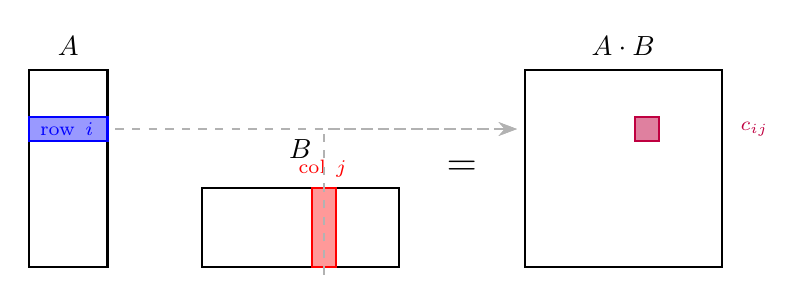
\begin{tikzpicture}[>=Stealth, thick, 
    highlight/.style={opacity=0.3},
    rowcolor/.style={fill=blue!40},
    colcolor/.style={fill=red!40},
    rescolor/.style={fill=purple!50}]

    % Matrix A (m x n) - Tall and thin
    % m = 2.5, n = 1.0
    \draw (0,0) rectangle (1.0, 2.5);
    \node at (0.5, 2.8) {$A$};
    
    % Highlight row i in A
    \fill[rowcolor] (0, 1.6) rectangle (1.0, 1.9);
    \draw[blue] (0, 1.6) rectangle (1.0, 1.9);
    \node[blue] at (0.5, 1.75) {\scriptsize row $i$};

    % Matrix B (n x p) - Short and wide
    % n = 1.0, p = 2.5
    \draw (2.2, 0) rectangle (4.7, 1.0);
    \node at (3.45, 1.5) {$B$};
    
    % Highlight col j in B
    \fill[colcolor] (3.6, 0) rectangle (3.9, 1.0);
    \draw[red] (3.6, 0) rectangle (3.9, 1.0);
    % Label col j placed above the red bar, avoiding overlap
    \node[red, anchor=south] at (3.75, 1.0) {\scriptsize col $j$};

    % Equals Sign
    \node at (5.5, 1.25) {\Large $=$};

    % Result Matrix AB (m x p) - Large square/rectangle
    % m = 2.5, p = 2.5
    \draw (6.3, 0) rectangle (8.8, 2.5);
    \node at (7.55, 2.8) {$A \cdot B$};
    
    % Highlight result cell c_ij
    \fill[rescolor] (7.7, 1.6) rectangle (8.0, 1.9);
    \draw[purple] (7.7, 1.6) rectangle (8.0, 1.9);
    \node[right=2pt, purple] at (8.8, 1.75) {\scriptsize $c_{ij}$};

    % Logical visualization arrows
    \draw[->, gray!60, dashed] (1.1, 1.75) -- (6.2, 1.75);
    \draw[->, gray!60, dashed] (3.75, -0.1) |- (6.2, 1.75);

\end{tikzpicture}
\end{center}
Another way to describe it is by considering the columns of $B$, denoted as $w_1, \dots, w_p$. The matrix $A \cdot B$ is then formed by multiplying $A$ with each column vector $w_j$:
\begin{equation*}
    A \cdot \begin{pmatrix} | & & | \\ w_1 & \dots & w_p \\ | & & | \end{pmatrix} = \begin{pmatrix} | & & | \\ A w_1 & \dots & A w_p \\ | & & | \end{pmatrix}
\end{equation*}

\begin{example}
We compute the product of a $2 \times 3$ matrix and a $3 \times 2$ matrix:
\begin{equation*}
    \begin{pmatrix} 3 & 2 & 1 \\ 1 & 0 & 2 \end{pmatrix} \cdot \begin{pmatrix} 1 & 2 \\ 0 & 1 \\ 4 & 0 \end{pmatrix} = \begin{pmatrix} 3 \cdot 1 + 2 \cdot 0 + 1 \cdot 4 & 3 \cdot 2 + 2 \cdot 1 + 1 \cdot 0 \\ 1 \cdot 1 + 0 \cdot 0 + 2 \cdot 4 & 1 \cdot 2 + 0 \cdot 1 + 2 \cdot 0 \end{pmatrix} = \begin{pmatrix} 7 & 8 \\ 9 & 2 \end{pmatrix}
\end{equation*}
Conversely, multiplying the $3 \times 2$ matrix by the $2 \times 3$ matrix yields a $3 \times 3$ matrix:
\begin{equation*}
    \begin{pmatrix} 1 & 2 \\ 0 & 1 \\ 4 & 0 \end{pmatrix} \cdot \begin{pmatrix} 3 & 2 & 1 \\ 1 & 0 & 2 \end{pmatrix} = \begin{pmatrix} 5 & 2 & 5 \\ 1 & 0 & 2 \\ 12 & 8 & 4 \end{pmatrix}
\end{equation*}
If $A \in \M_{m \times n}(K)$ and $B \in \M_{n \times p}(K)$, then $A \cdot B$ is defined, but $B \cdot A$ is not defined, unless $p = m$.
\end{example}

\subsection{Some Special Cases}

\begin{enumerate}
    \item If $A \in \M_{m \times n}(K)$ and $v \in K_{\text{col}}^{n}$, we have previously defined the matrix-vector product $A \cdot v \in K_{\text{col}}^{m}$. However, we can also identify $K_{\text{col}}^{n} = \M_{n \times 1}(K)$. If we view $v$ as an $n \times 1$ matrix, then the matrix multiplication of $A$ and $v$ yields the exact same result as applying $A$ to the vector $v$.
    
    \item If $A \in \M_{m \times n}(K)$ and $w \in K_{\text{row}}^{m} = \M_{1 \times m}(K)$, then we can define the left-multiplication $w \cdot A \in \M_{1 \times n}(K) = K_{\text{row}}^{n}$. If $A$ is represented by its row vectors $v_1, \dots, v_m$, this operation scales and sums the rows of $A$ according to the entries of $w$.
    
    \item Let $v = (a_1, \dots, a_n) \in K_{\text{row}}^{n} = \M_{1 \times n}(K)$, and let $w = (b_1, \dots, b_n)^T \in K_{\text{col}}^{n} = \M_{n \times 1}(K)$. Then the product $v \cdot w \in \M_{1 \times 1}(K) = K$ is simply the standard scalar product:
    \begin{equation*}
        v \cdot w = a_1 b_1 + \dots + a_n b_n
    \end{equation*}
\end{enumerate}

\subsection{Connections to Linear Maps}

As a conclusion from our previous discussions on linear maps, let $T: V \to W$ and $S: W \to U$ be linear maps between finite-dimensional vector spaces. Let $\mathcal{B}$, $\mathcal{C}$, and $\mathcal{E}$ be bases for $V$, $W$, and $U$, respectively. The matrix representation of the composition $S \circ T$ is given by the product of their respective representation matrices:
\[
    [S \circ T]_{\mathcal{E}}^{\mathcal{B}} = [S]_{\mathcal{E}}^{\mathcal{C}} \cdot [T]_{\mathcal{C}}^{\mathcal{B}}
\]

\begin{center}
\begin{tikzcd}[column sep=7em, row sep=4em, ampersand replacement=\&]
% Top row: Vector Spaces and Maps
V \arrow[r, "T"] \arrow[rr, bend left=25, "S \circ T"] \& W \arrow[r, "S"] \& U \\
% Bottom row: The bases associated with each space
\Sp(\mathcal{B}) \arrow[u, phantom, "\in", rotate=90, yshift=-0.3em] \& 
\Sp(\mathcal{C}) \arrow[u, phantom, "\in", rotate=90, yshift=-0.5em] \& 
\Sp(\mathcal{E}) \arrow[u, phantom, "\in", rotate=90, yshift=-0.3em]
\end{tikzcd}
\end{center}

\subsection{Notation and The Identity Matrix}

Let $\mathcal{I}$ be an index set. For $i, j \in \mathcal{I}$, we define the \textbf{Kronecker-delta} as:
\begin{equation*}
    \delta_{ij} := \begin{cases} 1 & \text{if } i = j \\ 0 & \text{if } i \neq j \end{cases}
\end{equation*}
Using this, we define the \qt{identity matrix} $I_n \in \M_{n \times n}(K)$ as $I_n = (\delta_{ij})_{\substack{1 \le i \le n \\ 1 \le j \le n}}$. Explicitly, this is:
\begin{equation*}
    I_n = \begin{pmatrix} 1 & & 0 \\ & \ddots & \\ 0 & & 1 \end{pmatrix}
\end{equation*}

\begin{remark}
Let $V$ be a finite-dimensional vector space, and let $n := \dim V$. Let $\id_V: V \to V$ be the identity map, and let $\mathcal{B}$ be any basis for $V$. Then, $[\id_V]_{\mathcal{B}}^{\mathcal{B}} = I_n$. In other words, the matrix representing the identity map with respect to the basis $\mathcal{B}$ is precisely the identity matrix $I_n$.
\end{remark}

\begin{exercise}
Prove the preceding remark.
\end{exercise}

\subsection{Properties of Matrix Multiplication}

\begin{proposition}[Algebraic Properties of Matrix Multiplication] 
% prop:17.a.2
\label{prop:matrix_multiplication_properties}
Matrix multiplication satisfies the following algebraic properties:
\begin{description}
    \item[Associativity:] For all $A \in \M_{m \times n}(K)$, $B \in \M_{n \times p}(K)$, and $C \in \M_{p \times q}(K)$, we have:
    \begin{equation*}
        (AB)C = A(BC) \in \M_{m \times q}(K)
    \end{equation*}
    \item[Distributivity:] For all $A, B \in \M_{m \times n}(K)$, $C \in \M_{n \times p}(K)$, and $C' \in \M_{q \times m}(K)$, we have:
    \begin{align*}
        (A + B)C &= AC + BC \in \M_{m \times p}(K) \\
        C'(A + B) &= C'A + C'B \in \M_{q \times n}(K)
    \end{align*}
    \item[Identity:] For all $A \in \M_{m \times n}(K)$, we have $I_m A = A$ and $A I_n = A$.
    \item[Scalar Multiplication:] For all $\alpha \in K$, $A \in \M_{m \times n}(K)$, and $B \in \M_{n \times p}(K)$, we have:
    \begin{equation*}
        \alpha(AB) = (\alpha A)B = A(\alpha B)
    \end{equation*}
\end{description}
\end{proposition}

\begin{proof}
Let $T_A: K^n \to K^m$, $T_B: K^p \to K^n$, and $T_C: K^q \to K^p$ be the linear maps defined by left-multiplication with the matrices $A$, $B$, and $C$, respectively (i.e., $T_A(v) = A \cdot v$ for all $v \in K^n$, $T_B(w) = B \cdot w$ for all $w \in K^p$, and $T_C(u) = C \cdot u$ for all $u \in K^q$). For any dimension $r$, we denote the standard basis of $K^r$ by $\mathcal{E}_r$. We have already established that:
\begin{equation*}
    [T_A]_{\mathcal{E}_n}^{\mathcal{E}_m} = A, \quad [T_B]_{\mathcal{E}_p}^{\mathcal{E}_n} = B, \quad \text{and} \quad [T_C]_{\mathcal{E}_q}^{\mathcal{E}_p} = C
\end{equation*}

\textbf{Proof of (a):} We rely on the associativity of function composition, which states that $(T_A \circ T_B) \circ T_C = T_A \circ (T_B \circ T_C)$. These are both maps from $K^q$ to $K^m$. We now pass to the matrix representation of these maps with respect to the standard bases $\mathcal{E}_q$ and $\mathcal{E}_m$:
\begin{equation*}
    [(T_A \circ T_B) \circ T_C]_{\mathcal{E}_q}^{\mathcal{E}_m} = [T_A \circ (T_B \circ T_C)]_{\mathcal{E}_q}^{\mathcal{E}_m}
\end{equation*}
By applying the rule for the matrix representation of composed maps, we get:
\begin{equation*}
    [T_A \circ T_B]_{\mathcal{E}_p}^{\mathcal{E}_m} \cdot [T_C]_{\mathcal{E}_q}^{\mathcal{E}_p} = [T_A]_{\mathcal{E}_n}^{\mathcal{E}_m} \cdot [T_B \circ T_C]_{\mathcal{E}_q}^{\mathcal{E}_n}
\end{equation*}
Expanding further, we obtain:
\begin{equation*}
    \left([T_A]_{\mathcal{E}_n}^{\mathcal{E}_m} \cdot [T_B]_{\mathcal{E}_p}^{\mathcal{E}_n}\right) \cdot [T_C]_{\mathcal{E}_q}^{\mathcal{E}_p} = [T_A]_{\mathcal{E}_n}^{\mathcal{E}_m} \cdot \left([T_B]_{\mathcal{E}_p}^{\mathcal{E}_n} \cdot [T_C]_{\mathcal{E}_q}^{\mathcal{E}_p}\right)
\end{equation*}
Substituting the matrices back in yields $(A \cdot B) \cdot C = A \cdot (B \cdot C)$.

\textbf{Proof of (b):} From the properties of linear maps, we know that $(T_A + T_B) \circ T_C = T_A \circ T_C + T_B \circ T_C$. Passing to the matrix representations, we have:
\begin{equation*}
    [(T_A + T_B) \circ T_C]_{\mathcal{E}_q}^{\mathcal{E}_m} = [T_A \circ T_C + T_B \circ T_C]_{\mathcal{E}_q}^{\mathcal{E}_m}
\end{equation*}
This implies that:
\begin{equation*}
    [T_A + T_B]_{\mathcal{E}_n}^{\mathcal{E}_m} \cdot [T_C]_{\mathcal{E}_q}^{\mathcal{E}_n} = [T_A \circ T_C]_{\mathcal{E}_q}^{\mathcal{E}_m} + [T_B \circ T_C]_{\mathcal{E}_q}^{\mathcal{E}_m}
\end{equation*}
Which directly gives us $(A + B) \cdot C = A \cdot C + B \cdot C$. The other distributive identity in (b) is proven similarly.

\textbf{Proof of (c):} The identity matrix $I_m$ represents the identity map: $I_m = [\id_{K^m}]_{\mathcal{E}_m}^{\mathcal{E}_m}$. Since composing with the identity map does not change a function, we have $\id_{K^m} \circ T_A = T_A$. Therefore:
\begin{equation*}
    [\id_{K^m} \circ T_A]_{\mathcal{E}_n}^{\mathcal{E}_m} = [T_A]_{\mathcal{E}_n}^{\mathcal{E}_m} = A
\end{equation*}
This implies that $I_m \cdot A = A$. The proof for $A I_n = A$ follows the same logic.

\textbf{Proof of (d):} Let $T_A: K^n \to K^m$ and $T_B: K^p \to K^n$ be the linear maps associated with $A$ and $B$, respectively. We want to show that $\alpha(AB) = (\alpha A)B = A(\alpha B)$. This is equivalent to showing that the corresponding linear maps are equal.

First, consider the map $Q: K^n \to K^n$ defined by $Q(v) := \alpha v$. This map is linear. If $\mathcal{E}_n$ is the standard basis for $K^n$, then for any $e_j \in \mathcal{E}_n$, $Q(e_j) = \alpha e_j$. Thus, the matrix representation of $Q$ with respect to $\mathcal{E}_n$ is $[Q]_{\mathcal{E}_n}^{\mathcal{E}_n} = \alpha I_n$.

Now, let's look at the compositions:
\begin{itemize}
    \item The linear map corresponding to $(\alpha A)B$ is $T_{\alpha A} \circ T_B$. We know that $T_{\alpha A}(v) = (\alpha A)v = \alpha(Av) = \alpha T_A(v)$, so $T_{\alpha A} = \alpha T_A$. Thus, $T_{(\alpha A)B} = (\alpha T_A) \circ T_B$.
    \item The linear map corresponding to $A(\alpha B)$ is $T_A \circ T_{\alpha B}$. Similarly, $T_{\alpha B} = \alpha T_B$. Thus, $T_{A(\alpha B)} = T_A \circ (\alpha T_B)$.
\end{itemize}

We need to show that $(\alpha T_A) \circ T_B = T_A \circ (\alpha T_B)$. For any $v \in K^p$:
\begin{align*}
    ((\alpha T_A) \circ T_B)(v) &= (\alpha T_A)(T_B(v)) \\
    &= \alpha (T_A(T_B(v))) \quad (\text{by definition of scalar multiplication for maps})
\end{align*}
And for the other side:
\begin{align*}
    (T_A \circ (\alpha T_B))(v) &= T_A((\alpha T_B)(v)) \\
    &= T_A(\alpha (T_B(v))) \quad (\text{by definition of scalar multiplication for maps}) \\
    &= \alpha (T_A(T_B(v))) \quad (\text{by linearity of } T_A)
\end{align*}
Since both compositions yield the same result, the corresponding matrices are equal: $(\alpha A)B = A(\alpha B)$.

Finally, to show $\alpha(AB) = (\alpha A)B$:
The matrix $\alpha(AB)$ corresponds to the linear map $\alpha(T_A \circ T_B)$.
The matrix $(\alpha A)B$ corresponds to the linear map $(\alpha T_A) \circ T_B$.
We have already shown that $(\alpha T_A) \circ T_B = \alpha (T_A \circ T_B)$ (from the first part of the derivation above).
Therefore, $\alpha(AB) = (\alpha A)B$.
\end{proof}

\begin{exercise}
The proof for statement (d) of Proposition \ref{prop:matrix_multiplication_properties} relies on the properties of scalar multiplication of linear maps. You are encouraged to verify these properties.
\end{exercise}

\begin{remark}
In the space $\M_{n \times n}(K)$, we can add and subtract matrices, and we can also multiply matrices. There is additionally a multiplicative unit $I_n$. Because these operations satisfy associativity, distributivity, and other relevant axioms, it follows that $\M_{n \times n}(K)$ forms a (non-com\-mu\-ta\-tive) ring with a unity.
\end{remark}

\begin{importantremark}
Matrix multiplication is, in general, \textbf{not commutative}. There exist matrices $A$ and $B$ such that $A \cdot B \neq B \cdot A$. For example:
\begin{align*}
    \begin{pmatrix} 1 & 0 \\ 0 & 0 \end{pmatrix} \cdot \begin{pmatrix} 0 & 0 \\ 1 & 0 \end{pmatrix} &= \begin{pmatrix} 0 & 0 \\ 0 & 0 \end{pmatrix} \\
    \begin{pmatrix} 0 & 0 \\ 1 & 0 \end{pmatrix} \cdot \begin{pmatrix} 1 & 0 \\ 0 & 0 \end{pmatrix} &= \begin{pmatrix} 0 & 0 \\ 1 & 0 \end{pmatrix}
\end{align*}
\end{importantremark}

\begin{remark}
In the space $\M_{n \times n}(K)$, we can add and subtract matrices, and we can also multiply matrices. There is additionally a multiplicative unit $I_n$. Because these operations satisfy associativity, distributivity, and other relevant axioms, it follows that $\M_{n \times n}(K)$ forms a (non-commutative) ring with a unity.
\end{remark}

\subsection{Invertible Matrices}

\begin{definition}[Invertibility]
An $n \times n$ matrix $A \in \M_{n \times n}(K)$ is called \qt{invertible} if there exists a matrix $B \in \M_{n \times n}(K)$ such that $A \cdot B = B \cdot A = I_n$.
\end{definition}

\begin{remark}
If $A$ is invertible, then there exists \textbf{only one} matrix $B$ such that $A \cdot B = B \cdot A = I_n$.
\end{remark}

\begin{proof}
Assume there are two matrices $B$ and $C$ such that $AB = BA = I_n$ and $AC = CA = I_n$. Then, we can calculate:
\begin{equation*}
    B = B \cdot I_n = B \cdot (A \cdot C) = (B \cdot A) \cdot C = I_n \cdot C = C
\end{equation*}
This proves the uniqueness.
\end{proof}

\begin{definition}[Inverse Matrix and the General Linear Group]
If $A$ is invertible, the unique matrix $B$ such that $AB = BA = I_n$ is called the \qt{inverse} of $A$ and is denoted by $A^{-1}$. We have:
\begin{equation*}
    A \cdot A^{-1} = A^{-1} \cdot A = I_n
\end{equation*}
\qt{The set of all invertible $n \times n$ matrices over $K$} is denoted by:
\begin{equation*}
    \GL_n(K) = \GL(n, K) := \{A \in \M_{n \times n}(K) \mid A \text{ is invertible}\}
\end{equation*}
\end{definition}

\begin{definition}[Group]
Let $G$ be a set and $\cdot : G \times G \to G$, $(a,b) \mapsto a \cdot b \in G$, be a binary operation. We say that $(G, \cdot)$ is a \textbf{group} if the following axioms hold:
Let $G$ be a set and $\cdot : G \times G \to G$, $(a,b) \mapsto a \cdot b \in G$, be a binary operation. We say that $(G, \cdot)$ is a \qt{group} if the following axioms hold:
\begin{enumerate}
    \item \textbf{Associativity:} For all $g_1, g_2, g_3 \in G$, we have $g_1 \cdot (g_2 \cdot g_3) = (g_1 \cdot g_2) \cdot g_3$.
    \item \textbf{Identity Element:} There exists an element $e \in G$ such that $e \cdot g = g \cdot e = g$ for all $g \in G$. The element $e$ is called the \qt{unit} (or \qt{identity}) of $G$.
    \item \textbf{Inverse Element:} For every $g \in G$, there exists an element $h \in G$ such that $g \cdot h = h \cdot g = e$. The element $h$ is called the \qt{inverse} of $g$.
\end{enumerate}
Furthermore, if $G$ satisfies $g_1 \cdot g_2 = g_2 \cdot g_1$ for all $g_1, g_2 \in G$, we say that $G$ is a \qt{commutative group} (or \qt{Abelian group}).
\end{definition}

\begin{proposition}[Group Properties]
% prop:17.a.6
\label{prop:group_basic_properties}
Let $G$ be a group. Then:
\begin{enumerate}
    \item The unit $e \in G$ is unique. (The unit $e$ is sometimes denoted as $1 \in G$.)
    \item For every $g \in G$, its inverse is uniquely defined. It is denoted by $g^{-1}$ (so that $g \cdot g^{-1} = g^{-1} \cdot g = e$).
    \item For every $g \in G$, we have $(g^{-1})^{-1} = g$.
    \item For all $g_1, g_2 \in G$, we have $(g_1 \cdot g_2)^{-1} = g_2^{-1} \cdot g_1^{-1}$.
\end{enumerate}
\end{proposition}

\begin{proposition}[The General Linear Group]
% prop:17.a.7
\label{prop:gl_group_structure}
The set $\GL_n(K)$, endowed with matrix multiplication $(A, B) \mapsto A \cdot B$, is a \qt{group}. The unity is the identity matrix $I_n$. The inverse of a matrix $A \in \GL_n(K)$ is $A^{-1}$. Moreover, for all $A, B \in \GL_n(K)$, we have:
\begin{equation*}
    (A^{-1})^{-1} = A \quad \text{and} \quad (AB)^{-1} = B^{-1}A^{-1}
\end{equation*}
\end{proposition}

\begin{proof}
Let $A, B \in \GL_n(K)$. To establish that $\GL_n(K)$ forms a group, we first need to show closure, namely that $AB \in \GL_n(K)$ as well. Indeed, we can verify this by checking the inverse property:
\begin{equation*}
    (B^{-1} \cdot A^{-1})(AB) = B^{-1}A^{-1}AB = B^{-1}I_nB = B^{-1}B = I_n
\end{equation*}
and, multiplying from the right,
\begin{equation*}
    (AB)(B^{-1}A^{-1}) = ABB^{-1}A^{-1} = AI_nA^{-1} = AA^{-1} = I_n
\end{equation*}
This proves that $AB$ is invertible with inverse $B^{-1}A^{-1}$, and therefore, $AB \in \GL_n(K)$. The other statements in the proposition follow immediately from what we have proved earlier regarding the uniqueness of inverses.
\end{proof}

\begin{corollary}[Unique Solution via Matrix Inverse]
% cor:17.a.8
\label{cor:unique_solution_via_inverse}
Let $A \in \GL_n(K)$. Then, for all $b \in K^n$, the linear system of equations $A \cdot x = b$ has a unique solution, namely $x = A^{-1} \cdot b$.
\end{corollary}

\begin{proof}
If $Ax = b$, then multiplying both sides from the left by $A^{-1}$ yields:
\begin{equation*}
    A^{-1}(Ax) = A^{-1}b \implies I_n x = A^{-1}b \implies x = A^{-1}b
\end{equation*}
Conversely, if we substitute $x = A^{-1}b$ into the equation, we obtain:
\begin{equation*}
    A(A^{-1}b) = (AA^{-1})b = I_n b = b
\end{equation*}
This confirms both the existence and uniqueness of the solution.
\end{proof}

\begin{proposition}[Equivalence of Invertibility and Isomorphism]
% prop:17.a.9
\label{prop:invertibility_isomorphism_equivalence}
Let $A \in \M_{n \times n}(K)$. Then, $A \in \GL_n(K)$ (i.e., $A$ is invertible) if and only if the associated linear map $T_A: K^n \to K^n$ is an isomorphism. Moreover, in this case, $(T_A)^{-1} = T_{A^{-1}}$.
\end{proposition}

\begin{proof}
First, assume that $A$ is invertible. We claim that $T_{A^{-1}} \circ T_A = \id_{K^n}$ and $T_A \circ T_{A^{-1}} = \id_{K^n}$, which will show that $T_A$ is an isomorphism. Indeed, for all $v \in K^n$:
\begin{equation*}
    T_{A^{-1}} \circ T_A(v) = A^{-1} \cdot (T_A(v)) = A^{-1} \cdot A \cdot v = I_n \cdot v = v
\end{equation*}
Similarly, one shows that for all $v \in K^n$:
\begin{equation*}
    T_A \circ T_{A^{-1}}(v) = I_n \cdot v = v
\end{equation*}
This proves that $T_A$ is an isomorphism.

Conversely, assume that $T_A: K^n \to K^n$ is an isomorphism. Let $S := (T_A)^{-1}$. By a previous result, we know that any linear map from $K^n$ to $K^n$ is given by left-multiplication with a matrix, so $S = T_B$ for some $B \in M_{n \times n}(K)$. Now, for all $w \in K^n$:
\begin{equation*}
    w = S \circ T_A(w) = T_B(A \cdot w) = B \cdot A \cdot w = (BA) \cdot w
\end{equation*}
We apply this equality for the standard basis vectors $w = e_1, w = e_2, \dots, w = e_n$ and obtain that $BA = I_n$. Similarly, using $T_A \circ S = \id_{K^n}$, one shows that $AB = I_n$ too. Thus, $A$ is invertible.
\end{proof}

\begin{exercise}
\begin{enumerate}
    \item Let $A \in \M_{m \times n}(K)$ and $B \in \M_{n \times p}(K)$. Prove that $(AB)^T = B^T \cdot A^T$. \newline (\textit{Hint: Proving this by direct calculation is not so bad.})
    \begin{proof}[Proof Sketch]
    Let $A = (a_{ij})$ and $B = (b_{jk})$. Let $C = AB = (c_{ik})$. Then $c_{ik} = \sum_{\ell=1}^n a_{i\ell} b_{\ell k}$.
    The $(i,k)$-th entry of $(AB)^T$ is $c_{ki} = \sum_{\ell=1}^n a_{k\ell} b_{\ell i}$.
    Now consider $B^T = (b'_{k\ell})$ where $b'_{k\ell} = b_{\ell k}$, and $A^T = (a'_{\ell i})$ where $a'_{\ell i} = a_{i\ell}$.
    The $(i,k)$-th entry of $B^T A^T$ is $\sum_{\ell=1}^n b'_{i\ell} a'_{\ell k} = \sum_{\ell=1}^n b_{\ell i} a_{k\ell}$.
    This is exactly $c_{ki}$, thus $(AB)^T = B^T A^T$.
    \end{proof}
    \item Let $A \in \GL_n(K)$. Prove that $A^T \in \GL_n(K)$ and that $(A^T)^{-1} = (A^{-1})^T$.
    \begin{proof}[Proof Sketch]
    For the first part, recall that $\det(A^T) = \det(A)$. Since $A \in \GL_n(K)$, we know $\det(A) \neq 0$, which implies $\det(A^T) \neq 0$, and thus $A^T \in \GL_n(K)$.
    For the second part, we need to show that $A^T (A^{-1})^T = I_n$ and $(A^{-1})^T A^T = I_n$. Using the result from part (1):
    \[ A^T (A^{-1})^T = (A^{-1}A)^T = I_n^T = I_n. \]
    Similarly,
    \[ (A^{-1})^T A^T = (AA^{-1})^T = I_n^T = I_n. \]
    This confirms that $(A^{-1})^T$ is indeed the inverse of $A^T$.
    \end{proof}
\end{enumerate}
\end{exercise}

\begin{definition}[Triangular and Diagonal Matrices]
% def:17.a.10
\label{def:triangular_diagonal_matrices}
A matrix $A \in \M_{n \times n}(K)$, with entries $A = (a_{ij})_{\substack{1 \le i \le n \\ 1 \le j \le n}}$, is called:
\begin{itemize}
    \item \qt{Upper triangular} if $a_{ij} = 0$ for all $i > j$.
    \item \qt{Lower triangular} if $a_{ij} = 0$ for all $i < j$.
    \item \qt{Diagonal} if $a_{ij} = 0$ for all $i \neq j$. A diagonal matrix has the form:
    \begin{equation*}
        \begin{pmatrix} * & & 0 \\ & \ddots & \\ 0 & & * \end{pmatrix}
    \end{equation*}
\end{itemize}
\end{definition}

\begin{lemma}[Closure of Triangular Matrices]
% lemma:17.a.11
\label{lemma:triangular_multiplication_closure}
Let $A$ and $B$ be two diagonal matrices (respectively, both upper triangular, or both lower triangular). Then, their product $A \cdot B$ is of the same type.
\end{lemma}

\begin{proof}
  Exercise: Let $A = (a_{ij})$ and $B = (b_{ij})$ be two upper triangular matrices. This means $a_{ij} = 0$ for $i > j$ and $b_{ij} = 0$ for $i > j$.
  Let $C = AB = (c_{ij})$. We want to show that $c_{ij} = 0$ for $i > j$.
  The entry $c_{ij}$ is given by the sum $c_{ij} = \sum_{k=1}^n a_{ik} b_{kj}$.

  Consider $c_{ij}$ where $i > j$. For each term $a_{ik} b_{kj}$ in the sum:
  \begin{itemize}
    \item If $k < i$: For $a_{ik}$ to be non-zero, $k$ must be less than or equal to $i$. If $k > j$, then $b_{kj}$ must be zero (since $B$ is upper triangular).
    \item If $k \ge i$: Since $i > j$, we have $k > j$. This implies $b_{kj} = 0$ (since $B$ is upper triangular).
  \end{itemize}
  More precisely, for $c_{ij}$ with $i > j$, we have $a_{ik} = 0$ for all $k < i$ such that $k < i$ is false (i.e., $k \ge i$), and $b_{kj} = 0$ for all $k > j$.
  Thus, in the sum $\sum_{k=1}^n a_{ik} b_{kj}$, if $k < i$, then $a_{ik}$ can be non-zero. But if $k > j$, $b_{kj}$ is zero. So we only need to consider $k \le j$.
  However, if $k \le j$ and $i > j$, then $i > k$. This means $a_{ik} = 0$ for all $k \le j$.
  Therefore, every term $a_{ik}b_{kj}$ in the sum must be zero when $i > j$. Hence, $c_{ij} = 0$ for $i > j$, and $C$ is upper triangular.
  The proofs for diagonal and lower triangular matrices follow similar logic.
\end{proof}

\section{Change of Basis}

\begin{question}
How does the representation matrix $[T]$ of a linear map $T: V \to W$ depend on the choices of bases $\mathcal{B}$ and $\mathcal{C}$?
\end{question}

\begin{corollary}[Change of Basis Formula]
% cor:17.b.1
\label{cor:change_of_basis_formula}
Let $V$ and $W$ be finite-di\-men\-sional vector spaces over $K$. Let $n := \dim V$ and $m := \dim W$. Let $\mathcal{B}$ and $\mathcal{B}'$ be two bases for $V$, and let $\mathcal{C}$ and $\mathcal{C}'$ be two bases for $W$. Then, $[\id_V]_{\mathcal{B}}^{\mathcal{B}'} \in \GL_n(K)$ and $[\id_W]_{\mathcal{C}}^{\mathcal{C}'} \in \GL_m(K)$, with inverses given by:
\begin{equation*}
    [\id_V]_{\mathcal{B}}^{\mathcal{B}'} = ([\id_V]_{\mathcal{B}'}^{\mathcal{B}})^{-1} \quad \text{and} \quad [\id_W]_{\mathcal{C}}^{\mathcal{C}'} = ([\id_W]_{\mathcal{C}'}^{\mathcal{C}})^{-1}
\end{equation*}
Let $T: V \to W$ be a linear map. Then, its representation matrix changes according to the formula:
\begin{equation*}
    [T]_{\mathcal{C}'}^{\mathcal{B}'} = [\id_W]_{\mathcal{C}'}^{\mathcal{C}} \cdot [T]_{\mathcal{C}}^{\mathcal{B}} \cdot [\id_V]_{\mathcal{B}}^{\mathcal{B}'}
\end{equation*}
\end{corollary}

\begin{proof}
We can write $T$ as the composition $T = \id_W \circ T \circ \id_V = \id_W \circ (T \circ \id_V)$. Passing to the matrix representations, this yields:
\begin{equation*}
    [T]_{\mathcal{C}'}^{\mathcal{B}'} = [\id_W]_{\mathcal{C}'}^{\mathcal{C}} \cdot [T \circ \id_V]_{\mathcal{C}}^{\mathcal{B}'} = [\id_W]_{\mathcal{C}'}^{\mathcal{C}} \cdot [T]_{\mathcal{C}}^{\mathcal{B}} \cdot [\id_V]_{\mathcal{B}}^{\mathcal{B}'}
\end{equation*}
Also, we have the identity $\id_V = \id_V \circ \id_V$. This implies that:
\begin{equation*}
    I_n = [\id_V]_{\mathcal{B}}^{\mathcal{B}} = [\id_V]_{\mathcal{B}}^{\mathcal{B}'} \cdot [\id_V]_{\mathcal{B}'}^{\mathcal{B}}
\end{equation*}
and similarly:
\begin{equation*}
    I_n = [\id_V]_{\mathcal{B}'}^{\mathcal{B}'} = [\id_V]_{\mathcal{B}'}^{\mathcal{B}} \cdot [\id_V]_{\mathcal{B}}^{\mathcal{B}'}
\end{equation*}
This demonstrates that $[\id_V]_{\mathcal{B}}^{\mathcal{B}'}$ is invertible and that its inverse is indeed $([\id_V]_{\mathcal{B}'}^{\mathcal{B}})^{-1}$. The proof for $[\id_W]_{\mathcal{C}}^{\mathcal{C}'}$ follows the exact same logic.
\end{proof}

\begin{definition}[Change of Basis Matrix]
% def:17.b.2
\label{def:change_of_basis_matrix}
Let $V$ be a finite-di\-men\-sional vector space over $K$, and let $n := \dim V$. Let $\mathcal{B}$ and $\mathcal{B}'$ be two bases of $V$. The matrix $[\id_V]_{\mathcal{B}'}^{\mathcal{B}} \in \GL_n(K)$ is called the \qt{change of basis matrix} between $\mathcal{B}$ and $\mathcal{B}'$, or the \qt{transition matrix} from basis $\mathcal{B}$ to basis $\mathcal{B}'$.
\end{definition}

\begin{remark}
If $\mathcal{B} = (w_1, \dots, w_n)$ and $\mathcal{B}' = (w_1', \dots, w_n')$, then the transition matrix is explicitly constructed by placing the coordinate vectors of the old basis elements with respect to the new basis into the columns:
\begin{equation*}
    [\id_V]_{\mathcal{B}'}^{\mathcal{B}} = \begin{pmatrix} | & & | \\ [w_1]_{\mathcal{B}'} & \dots & [w_n]_{\mathcal{B}'} \\ | & & | \end{pmatrix}
\end{equation*}
\end{remark}

\begin{proposition}[Representation of Isomorphisms]
% prop:17.b.3
\label{prop:representation_of_isomorphisms}
Let $T: V \to W$ be an isomorphism between two finite-di\-men\-sional vector spaces. Let $\mathcal{B}$ and $\mathcal{C}$ be bases for $V$ and $W$, respectively. Then, the matrix $[T]_{\mathcal{C}}^{\mathcal{B}}$ is an invertible matrix, and furthermore:
\begin{equation*}
    [T^{-1}]_{\mathcal{B}}^{\mathcal{C}} = ([T]_{\mathcal{C}}^{\mathcal{B}})^{-1}
\end{equation*}
\end{proposition}

\begin{proof}
Let $n := \dim V = \dim W$. By the properties of composed linear maps and representation matrices, we have:
\begin{equation*}
    [T^{-1}]_{\mathcal{B}}^{\mathcal{C}} \cdot [T]_{\mathcal{C}}^{\mathcal{B}} = [\id_V]_{\mathcal{B}}^{\mathcal{B}} = I_n
\end{equation*}
and conversely:
\begin{equation*}
    [T]_{\mathcal{C}}^{\mathcal{B}} \cdot [T^{-1}]_{\mathcal{B}}^{\mathcal{C}} = [\id_W]_{\mathcal{C}}^{\mathcal{C}} = I_n
\end{equation*}
This proves the claim.
\end{proof}

\subsection{Equivalence and Similarity of Matrices}

\begin{question}
Suppose $T: V \to V$ is an endomorphism. Let $\mathcal{B}$ and $\mathcal{B}'$ be two bases for $V$. What is the relation between $[T]_{\mathcal{B}'}^{\mathcal{B}'}$ and $[T]_{\mathcal{B}}^{\mathcal{B}}$?
\end{question}

\begin{corollary}[Similarity of Representation Matrices]
% cor:17.b.4
\label{cor:similarity_of_representation_matrices}
Let $V$ be a finite-di\-men\-sional vector space, and let $T: V \to V$ be a linear map. Let $\mathcal{B}$ and $\mathcal{B}'$ be two bases for $V$. Then:
\begin{equation*}
    [T]_{\mathcal{B}'}^{\mathcal{B}'} = [\id_V]_{\mathcal{B}'}^{\mathcal{B}} \cdot [T]_{\mathcal{B}}^{\mathcal{B}} \cdot [\id_V]_{\mathcal{B}}^{\mathcal{B}'} = ([\id_V]_{\mathcal{B}}^{\mathcal{B}'})^{-1} \cdot [T]_{\mathcal{B}}^{\mathcal{B}} \cdot [\id_V]_{\mathcal{B}}^{\mathcal{B}'}
\end{equation*}
\end{corollary}

\begin{definition}[Equivalence and Similarity]
% def:17.b.5
\label{def:equivalence_and_similarity}
We define two types of relations between matrices:
\begin{enumerate}
    \item Let $A, B \in \M_{m \times n}(K)$. We say that $A$ and $B$ are \qt{equivalent} if there exist matrices $P \in \GL_m(K)$ and $Q \in \GL_n(K)$ such that $B = P A Q$.
    \item Let $A, B \in \M_{n \times n}(K)$. We say that $A$ and $B$ are \qt{similar} if there exists a matrix $P \in \GL_n(K)$ such that $B = P^{-1} A P$.
\end{enumerate}
\end{definition}

\begin{exercise}
\begin{enumerate}
    \item Show that \qt{equivalence} between $m \times n$ matrices defines an equivalence relation on $\M_{m \times n}(K)$.
    \item Show that two matrices $A, B \in \M_{m \times n}(K)$ are equivalent if and only if there exist two vector spaces $V$ and $W$ with $\dim V = n$ and $\dim W = m$, two bases $\mathcal{B}$ and $\mathcal{B}'$ of $V$, and two bases $\mathcal{C}$ and $\mathcal{C}'$ of $W$ such that:
    \begin{equation*}
        A = [T]_{\mathcal{C}}^{\mathcal{B}} \quad \text{and} \quad B = [T]_{\mathcal{C}'}^{\mathcal{B}'}
    \end{equation*}
    In other words, $A$ is equivalent to $B$ if and only if $A$ and $B$ are matrix representations of the exact same linear map $T$, but with respect to different choices of bases for $V$ and $W$.
    \item Show that \qt{similarity} between $n \times n$ matrices defines an equivalence relation on $\M_{n \times n}(K)$.
    \item Show that two square matrices $M, N \in \M_{n \times n}(K)$ are similar if and only if there exists an $n$-di\-men\-sional space $V$, an endomorphism $T: V \to V$, and two bases $\mathcal{B}$ and $\mathcal{B}'$ of $V$ such that $M = [T]_{\mathcal{B}}^{\mathcal{B}}$ and $N = [T]_{\mathcal{B}'}^{\mathcal{B}'}$.
\end{enumerate}
\end{exercise}

\begin{proposition}[Normal Form for Linear Maps]
% prop:17.b.6
\label{prop:linear_map_normal_form}
Let $V$ and $W$ be finite-di\-men\-sional vector spaces over $K$, with dimensions $n = \dim V$ and $m = \dim W$. Let $T: V \to W$ be a linear map with $\rank(T) = r$. (Recall that $\rank(T) := \dim \operatorname{Im}(T)$). Then, there exists a basis $\mathcal{B} = (v_1, \dots, v_n)$ of $V$ and a basis $\mathcal{C} = (w_1, \dots, w_m)$ of $W$ such that:
\begin{equation*}
    [T]_{\mathcal{C}}^{\mathcal{B}} = \begin{pmatrix} I_r & O_{r, n-r} \\ O_{m-r, r} & O_{m-r, n-r} \end{pmatrix}
\end{equation*}
where $O_{p,q}$ stands for the zero matrix in $M_{p \times q}(K)$.
\end{proposition}

\begin{proof}
Put $\ell := \dim \ker(T)$. By the rank theorem, we know that $r = n - \ell$. Let $v_1, \dots, v_\ell$ be a basis of $\ker(T)$, and extend it to a full basis $(v_1, \dots, v_\ell, v_{\ell+1}, \dots, v_n)$ of $V$. It will be useful to work below with the rearranged basis:
\begin{equation*}
    \mathcal{B} = (v_{\ell+1}, \dots, v_n, v_1, \dots, v_\ell)
\end{equation*}
In the proof of the rank theorem, we have seen that $T(v_{\ell+1}), \dots, T(v_n)$ form a basis for $\operatorname{Im}(T)$. Define $w_i := T(v_{\ell+i})$ for $i = 1, \dots, r$ (i.e., $w_1 = T(v_{\ell+1}), \dots, w_r = T(v_{\ell+r})$), and extend this list to a basis of $W$:
\begin{equation*}
    \mathcal{C} := (w_1, \dots, w_r, w_{r+1}, \dots, w_m)
\end{equation*}
It now directly follows from these definitions that the representation matrix $[T]_{\mathcal{C}}^{\mathcal{B}}$ takes the exact block form described in the proposition.
\end{proof}

\begin{corollary}[Matrix Equivalence and Normal Form]
% cor:17.b.7
\label{cor:matrix_equivalence_normal_form}
Let $A \in \M_{m \times n}(K)$. Then, there exist invertible matrices $P \in \GL_m(K)$ and $Q \in \GL_n(K)$ such that:
\begin{equation*}
    PAQ = \begin{pmatrix} I_r & O \\ O & O \end{pmatrix}
\end{equation*}
where $r = \rank_{\text{col}}(A)$. In particular, $\rank_{\text{col}}(A) \le \min\{m, n\}$.
\end{corollary}

\begin{proof}
Consider the linear map $T_A: K^n \to K^m$ defined by left-multiplication, $T_A(v) = A \cdot v$. Then, $r = \rank_{\text{col}}(A) = \dim \operatorname{Im}(T_A)$, because we have previously seen that 
\[\operatorname{Im}(T_A) = \operatorname{Sp}(T_A(e_1), \dots, T_A(e_n)) = \operatorname{Sp}(\text{columns of } A).\]

Now, we apply the previous proposition to $T_A$, yielding that:
\begin{equation*}
    [T_A]_{\mathcal{C}}^{\mathcal{B}} = \begin{pmatrix} I_r & O \\ O & O \end{pmatrix}
\end{equation*}
for some basis $\mathcal{B}$ of $K^n$ and some basis $\mathcal{C}$ of $K^m$. Using the change of basis formula, we can rewrite this as:
\begin{equation*}
    \underbrace{[\id_{K^m}]_{\mathcal{E}_m}^{\mathcal{C}}}_{=: P} \cdot \underbrace{[T_A]_{\mathcal{E}_m}^{\mathcal{E}_n}}_{= A} \cdot \underbrace{[\id_{K^n}]_{\mathcal{E}_n}^{\mathcal{B}}}_{=: Q} = \begin{pmatrix} I_r & O \\ O & O \end{pmatrix}
\end{equation*}
where $\mathcal{E}_n$ and $\mathcal{E}_m$ are the standard bases of $K^n$ and $K^m$, respectively. Setting $P = [\id_{K^m}]_{\mathcal{E}_m}^{\mathcal{C}}$ and $Q = [\id_{K^n}]_{\mathcal{E}_n}^{\mathcal{B}}$ concludes the proof.
\end{proof}

\begin{remark}
The fact that $\rank_{\text{col}}(A) \le \min\{m, n\}$ also follows from observing the linear map $T_A: K^n \to K^m$. We have:
\begin{equation*}
    \rank_{\text{col}}(A) = \dim \operatorname{Im}(T_A) = n - \dim \ker(T_A) \le n
\end{equation*}
and simultaneously,
\begin{equation*}
    \rank_{\text{col}}(A) = \dim \operatorname{Im}(T_A) \le \dim K^m = m
\end{equation*}
\end{remark}

\begin{question}
Recall that we have an equivalence relation on $M_{m \times n}(K)$: $A \sim B$ if there exist $P \in GL_m(K)$ and $Q \in GL_n(K)$ such that $B = PAQ$. Can we describe the equivalence classes of this equivalence relation?
\end{question}

\begin{corollary}[Classification of Matrices by Rank]
% cor:17.b.8
\label{cor:matrix_rank_equivalence_classification}
Let $A, B \in \M_{m \times n}(K)$. Then, $A \sim B$ if and only if $\rank_{\text{col}}(A) = \rank_{\text{col}}(B)$. Moreover, for every $0 \le r \le \min\{m, n\}$, there is precisely one equivalence class of matrices $A$ with $\rank_{\text{col}} = r$.
\end{corollary}

\begin{proof}
Let $A, B \in \M_{m \times n}(K)$. First, assume that $\rank_{\text{col}}(A) = \rank_{\text{col}}(B)$, and denote this common column rank by $r$. By Corollary \ref{cor:matrix_equivalence_normal_form}, we know that $A \sim \begin{pmatrix} I_r & 0 \\ 0 & 0 \end{pmatrix}$ and $B \sim \begin{pmatrix} I_r & 0 \\ 0 & 0 \end{pmatrix}$. Since $\sim$ is an equivalence relation, it naturally follows that $A \sim B$.

Conversely, assume that $A \sim B$. This implies that there exist matrices $P \in GL_m(K)$ and $Q \in GL_n(K)$ such that $B = PAQ$. Transitioning to the associated linear maps, this means $T_B = T_P \circ T_A \circ T_Q$. We analyze the image of $T_B$:
\begin{equation*}
    \operatorname{Im}(T_B) = T_B(K^n) = T_P \circ T_A(T_Q(K^n)) = T_P \circ T_A(K^n) = T_P(\operatorname{Im}(T_A))
\end{equation*}
Note that $T_Q(K^n) = K^n$ because $T_Q$ is an isomorphism. Consequently, the dimension of the image is:
\begin{equation*}
    \rank_{\text{col}}(B) = \dim \operatorname{Im}(T_B) = \dim T_P(\operatorname{Im}(T_A)) = \dim \operatorname{Im}(T_A) = \rank_{\text{col}}(A)
\end{equation*}
where the second to last equality holds because $T_P$ is an isomorphism, preserving the dimension of subspaces.
\end{proof}
\section{Column Rank and Row Rank}

\begin{theorem}[Equality of Column and Row Rank]
% thm:17.c.1
\label{thm:rank_row_column_equality}
Let $A \in \M_{m \times n}(K)$. Then, $\rank_{\text{col}}(A) = \rank_{\text{row}}(A)$.
\end{theorem}

\begin{remark}[Notation and Properties of Rank]
\begin{enumerate}
    \item Because of this theorem, we will from now on denote $\rank(A) := \rank_{\text{col}}(A) = \rank_{\text{row}}(A)$.
    \item Suppose $A'$ is a row-reduced echelon matrix that is row-equivalent to $A$. Then, we have:
    \begin{equation*}
        \rank(A) = \rank_{\text{row}}(A) = \rank_{\text{row}}(A') = \text{number of pivots in } A'
    \end{equation*}
    \item Recall that for a linear map $T: V \to W$, we defined $\rank(T) := \dim \operatorname{Im}(T)$. Moreover, if $A \in \M_{m \times n}(K)$, then $\rank(T_A) = \dim \operatorname{Im}(T_A) = \rank_{\text{col}}(A)$.
\end{enumerate}
\end{remark}

\subsection{Preparation for the Proof}

\begin{lemma}[Rank Invariance under Composition with Isomorphisms]
% lemma:17.c.2
\label{lemma:rank_invariance_isomorphisms}
Let $T: V \to W$ be a linear map, and let $S: W \to W'$ and $L: P \to V$ be isomorphisms. Then:
\begin{enumerate}
    \item $\rank(S \circ T) = \rank(T)$.
    \item $\rank(T \circ L) = \rank(T)$.
\end{enumerate}
\end{lemma}

\begin{proof}
\textbf{Proof of (a):} By definition, $\rank(S \circ T) = \dim (S(T(V)))$. Since $S$ is an isomorphism, its restriction to the subspace $T(V) \subseteq W$ is injective. An injective linear map preserves the dimension of a vector space, and therefore:
\begin{equation*}
    \dim (S(T(V))) = \dim (T(V)) = \rank(T)
\end{equation*}

\textbf{Proof of (b):} By definition, $\rank(T \circ L) = \dim (T(L(P)))$. Since $L$ is an isomorphism, it is surjective, which implies that $L(P) = V$. Consequently:
\begin{equation*}
    \dim (T(L(P))) = \dim (T(V)) = \rank(T)
\end{equation*}
This completes the proof.
\end{proof}

\begin{lemma}[Invertibility of the Transpose]
% lemma:17.c.3
\label{lemma:transpose_invertibility}
Let $A \in \M_{n \times n}(K)$. Then, $A \in \GL_n(K)$ if and only if $A^T \in \GL_n(K)$.
\end{lemma}

\begin{proof}
We know that $A$ is invertible if and only if the associated linear map $T_A: K^n \to K^n$ is an isomorphism. This is true if and only if $\rank(T_A) = n$, which is equivalent to $\rank_{\text{col}}(A) = n$.

We also know that $A$ is row-equivalent to some row-reduced echelon matrix $A'$. Since row-equivalence corresponds to multiplying from the left by invertible matrices, we have that $A \in GL_n(K)$ if and only if $A' \in GL_n(K)$. Because $A'$ is an $n \times n$ row-reduced echelon matrix, $A'$ is invertible if and only if it has no zero rows. This holds if and only if $A'$ has $n$ pivots, which is equivalent to $\rank_{\text{row}}(A') = n$. Since row operations preserve the row space, this means $\rank_{\text{row}}(A) = n$.

In summary, we have established that $A \in \GL_n(K)$ if and only if $\rank_{\text{row}}(A) = n$. But by definition, the row rank of $A$ is exactly the column rank of its transpose, so $\rank_{\text{row}}(A) = \rank_{\text{col}}(A^T)$. Therefore, $A \in \GL_n(K)$ if and only if $\rank_{\text{col}}(A^T) = n$, which means $A^T$ is invertible.
\end{proof}

\begin{lemma}[Rank Invariance under Matrix Equivalence]
% lemma:17.c.4
\label{lemma:rank_invariance_equivalence}
Let $A, B \in \M_{m \times n}(K)$ such that $B = P A Q$, where $P \in \GL_m(K)$ and $Q \in \GL_n(K)$. Then:
\begin{enumerate}
    \item $\rank_{\text{col}}(A) = \rank_{\text{col}}(B)$.
    \item $\rank_{\text{row}}(A) = \rank_{\text{row}}(B)$.
\end{enumerate}
\end{lemma}

\begin{proof}
\textbf{Proof of (a):} Transitioning to the associated linear maps, we have $T_B = T_P \circ T_A \circ T_Q$. Since $P$ and $Q$ are invertible matrices, both $T_P$ and $T_Q$ are isomorphisms. Applying Lemma \ref{lemma:rank_invariance_isomorphisms}, we deduce that $\rank(T_B) = \rank(T_A)$. Recalling that the rank of a linear map given by a matrix matches the column rank of that matrix, we obtain $\rank_{\text{col}}(B) = \rank_{\text{col}}(A)$.

\textbf{Proof of (b):} Taking the transpose of the equation $B = PAQ$ yields $B^T = Q^T A^T P^T$. Since $P$ and $Q$ are invertible matrices, their transposes $P^T$ and $Q^T$ are also invertible (we have previously seen that $(P^T)^{-1} = (P^{-1})^T$). We can now apply part (a) of this Lemma, which we have already proven, to the matrices $A^T$ and $B^T$. This gives us $\rank_{\text{col}}(B^T) = \rank_{\text{col}}(A^T)$. By the definition of the transpose, this immediately translates to $\rank_{\text{row}}(B) = \rank_{\text{row}}(A)$.
\end{proof}

\subsection{Proof of the Main Theorem}

We are now ready for the proof of Theorem \ref{thm:rank_row_column_equality}.

\begin{proof}[Proof of Theorem \ref{thm:rank_row_column_equality}]
Let $r := \rank_{\text{col}}(A)$. By a previous proposition regarding the equivalence of matrices, we know that there exist invertible matrices $P \in GL_m(K)$ and $Q \in GL_n(K)$ such that:
\begin{equation*}
    P A Q = \begin{pmatrix} I_r & O \\ O & O \end{pmatrix} =: B
\end{equation*}
By Lemma \ref{lemma:17.c.4}, we know that $\rank_{\text{row}}(A) = \rank_{\text{row}}(B)$. Thus, it suffices to determine the row rank of $B$.

The matrix $B$ is of the block form $\left(\begin{smallmatrix} I_r & O \\ O & O \end{smallmatrix}\right)$. The non-zero rows of $B$ are precisely the first $r$ standard basis vectors $e_1^T, e_2^T, \dots, e_r^T \in K_{\text{row}}^n$. Since these vectors form a linearly independent set, the dimension of the row space of $B$ is exactly $r$. Consequently, $\rank_{\text{row}}(B) = r$.

Therefore, we conclude that $\rank_{\text{row}}(A) = r = \rank_{\text{col}}(A)$, completing the proof.
\end{proof}

\begin{importantremark}[Column Space versus Row Space]
Although $\rank_{\text{col}}(A) = \rank_{\text{row}}(A)$, the column space and the row space are, in general, different vector spaces. First of all, if $A \in \M_{m \times n}(K)$, then the column space is a subspace of $K^m$, whereas the row space is a subspace of $K_{\text{row}}^n$ (which is isomorphic to $K^n$). But even in the case where $m = n$ (i.e., $A \in \M_{n \times n}(K)$), these two spaces are generally distinct! They share the exact same dimension, but they are not the same space.
\end{importantremark}
\section{More on Matrices and Linear Equations}

Let $A \in \M_{m \times n}(K)$, and consider the homogeneous system of linear equations $A \cdot x = 0$. We denote the space of solutions of this system by:
\begin{equation*}
    \operatorname{Sol}(A, 0) := \{x \in K^n \mid A x = 0\} = \ker(T_A)
\end{equation*}
Note that by the Rank-Nullity Theorem, we have 
\[\dim \operatorname{Sol}(A, 0) = n - \rank(A),\] 
because $\dim \ker(T_A) = n - \dim \operatorname{Im}(T_A)$.

Let $A'$ be a row-reduced echelon matrix that is row-equivalent to $A$ (for example, $A'$ is obtained from $A$ by Gauss elimination). We then know that the number of pivots of $A'$ equals $\rank(A)$, and the number of free variables is $n - \rank(A)$.

We can visualize the structure of $A'$ and its corresponding variables $x_1, \dots, x_n$ as follows. The columns containing the leading $1$'s (pivots) correspond to the pivot variables, while the remaining columns correspond to the free variables. Clearly, the solution spaces are identical:
\begin{equation*}
    \operatorname{Sol}(A, 0) = \operatorname{Sol}(A', 0)
\end{equation*}

Denote by $x_{i_1}, \dots, x_{i_\ell}$ the free variables, where $1 \le i_1 < \dots < i_\ell \le n$ and $\ell = n - \rank(A)$. Similarly, denote by $x_{j_1}, \dots, x_{j_r}$ the pivot variables, where $1 \le j_1 < \dots < j_r \le n$ and $r = \rank(A)$.

For each choice of values for the free variables $x_{i_1}, \dots, x_{i_\ell} \in K$, the pivot variables $x_{j_1}, \dots, x_{j_r}$ are uniquely determined. So, we obtain a map $\Phi: K^\ell \to \operatorname{Sol}(A, 0)$, where $\ell = n - \rank(A)$, defined by:
\begin{equation*}
    \Phi(\lambda_1, \dots, \lambda_\ell) = \text{the unique solution of } Ax = 0 \text{ (which is the solution of } A'x = 0 \text{)}
\end{equation*}
with $x_{i_1} = \lambda_1, \dots, x_{i_k} = \lambda_k, \dots, x_{i_\ell} = \lambda_\ell$.

\begin{proposition}[Linearity and Isomorphism of the Solution Map]
% prop:17.d.1
\label{prop:solution_map_isomorphism}
The map $\Phi$ is linear. Moreover, it is an isomorphism.
\end{proposition}

\begin{proof}
\textbf{Linearity of $\Phi$:} The $k$-th non-zero row of $A'$ gives the following equation:
\begin{equation*}
    x_{j_k} + (\text{linear combination of the free variables that come after } j_k) = 0
\end{equation*}
This allows us to isolate the pivot variable $x_{j_k}$:
\begin{equation*}
    x_{j_k} = - \sum_{\{q \mid 1 \le q \le \ell, \, i_q > j_k\}} a'_{k, i_q} \cdot x_{i_q}
\end{equation*}
This explicitly shows that the pivot variables $x_{j_1}, \dots, x_{j_r}$ depend linearly on the free variables $x_{i_1}, \dots, x_{i_\ell}$. This proves the linearity of $\Phi$.

\textbf{Isomorphism:} To prove that $\Phi$ is an isomorphism, it is enough to show that $\ker(\Phi) = \{0\}$, because $\Phi: K^\ell \to \operatorname{Sol}(A, 0)$ is a linear map between two spaces of the exact same dimension $\ell$.

But this clearly holds: if $\lambda = (\lambda_1, \dots, \lambda_\ell) \in \ker(\Phi)$, which means $\Phi(\lambda_1, \dots, \lambda_\ell) = 0$, then by the definition of $\Phi$, we must have $\lambda_1 = \dots = \lambda_\ell = 0$. This is simply because each $\lambda_k$ is an actual entry in the output vector $\Phi(\lambda_1, \dots, \lambda_\ell)$.

Furthermore, we can explicitly state the inverse map $\Phi^{-1}$. For any $x \in \operatorname{Sol}(A, 0)$, we extract the entries corresponding to the free variables:
\begin{equation*}
    \Phi^{-1}(x) = \begin{pmatrix} x_{i_1} \\ \vdots \\ x_{i_\ell} \end{pmatrix}
\end{equation*}
This completes the proof.
\end{proof}

\begin{corollary}[Structure of Non-Homogeneous Solutions]
% cor:17.d.2
\label{cor:non_homogeneous_solutions}
Let $b \in K^m$, and $A \in \M_{m \times n}(K)$. Then:
\begin{enumerate}
    \item $\operatorname{Sol}(A, b) := \{x \in K^n \mid A \cdot x = b\} \neq \emptyset$ if and only if $b \in \operatorname{ColS}(A)$.
    \item If $\operatorname{Sol}(A, b) \neq \emptyset$ and $y \in \operatorname{Sol}(A, b)$, then:
    \begin{equation*}
        \operatorname{Sol}(A, b) = y + \operatorname{Sol}(A, 0) := \{y + x \mid x \in \operatorname{Sol}(A, 0)\}
    \end{equation*}
\end{enumerate}
\end{corollary}

\begin{proof}
This is left as an exercise.

\textbf{Hints:}
1) Write the matrix $A$ in terms of its column vectors $v_1, \dots, v_n$:
\begin{equation*}
    A = \begin{pmatrix} | & & | \\ v_1 & \dots & v_n \\ | & & | \end{pmatrix}
\end{equation*}
For any vector $x = \begin{pmatrix} x_1 \\ \vdots \\ x_n \end{pmatrix} \in K^n$, the matrix-vector product is a linear combination of the columns:
\begin{equation*}
    A \cdot x = x_1 \begin{pmatrix} | \\ v_1 \\ | \end{pmatrix} + \dots + x_n \begin{pmatrix} | \\ v_n \\ | \end{pmatrix}
\end{equation*}

2) Let $y \in \operatorname{Sol}(A, b)$. First, assume $x \in \operatorname{Sol}(A, 0)$. Then $A \cdot x = 0$ and $A \cdot y = b$. Adding these together yields:
\begin{equation*}
    A(y + x) = A \cdot y + A \cdot x = b + 0 = b
\end{equation*}
Conversely, if $z \in \operatorname{Sol}(A, b)$, meaning $A \cdot z = b$, then define $x := z - y$. We obviously have $z = y + x$, and checking the multiplication gives:
\begin{equation*}
    A \cdot x = A \cdot (z - y) = A \cdot z - A \cdot y = b - b = 0
\end{equation*}
This shows that any solution $z$ can be written as $y + x$ for some $x \in \operatorname{Sol}(A, 0)$.
\end{proof}

\begin{proposition}[Rank Criterion for Solvability]
% prop:17.d.3
\label{prop:rank_solvability_criterion}
Let $A \in \M_{m \times n}(K)$ and $b \in K^m$. The following statements are equivalent:
\begin{enumerate}
    \item $\rank(A|b) = \rank(A)$.
    \item The system of equations $Ax = b$ has a solution.
\end{enumerate}
\end{proposition}

\begin{proof}
Write $A$ in terms of its columns, $A = \begin{pmatrix} | & & | \\ v_1 & \dots & v_n \\ | & & | \end{pmatrix}$. We have the following chain of equivalences:
\begin{align*}
    \rank(A|b) = \rank(A) &\iff \operatorname{col-rank}(A|b) = \operatorname{col-rank}(A) \\
    &\iff \dim \Sp(v_1, \dots, v_n, b) = \dim \Sp(v_1, \dots, v_n) \\
    &\iff b \in \Sp(v_1, \dots, v_n) \\
    &\iff b \in \operatorname{ColS}(A) \\
    &\iff \operatorname{Sol}(A, b) \neq \emptyset
\end{align*}
The last step holds directly by Corollary \ref{cor:non_homogeneous_solutions}, thus finishing the proof.
\end{proof}

\begin{proposition}[Criterion for a Unique Solution]
% prop:17.d.4
\label{prop:unique_solution_rank_criterion}
Let $A \in \M_{m \times n}(K)$ and $b \in K^m$. The following statements are equivalent:
\begin{enumerate}
    \item $\rank(A) = \rank(A|b) = n$.
    \item The system $Ax = b$ has a unique solution.
\end{enumerate}
\end{proposition}

\begin{proof}
This is left as an exercise.

\textbf{Hints:} Write $A = \begin{pmatrix} | & & | \\ v_1 & \dots & v_n \\ | & & | \end{pmatrix}$. Note that:
\begin{equation*}
    \rank(A) = n \iff \dim \Sp(v_1, \dots, v_n) = n
\end{equation*}
Since there are $n$ column vectors, this means that $v_1, \dots, v_n$ are linearly independent, and therefore, they form a basis for $\operatorname{ColS}(A)$.
\end{proof}
\section{Elementary Row Operations Revisited}

Let $A \in \M_{n \times p}(K)$. We have previously learned about elementary row operations, which are utilized as an integral part of the Gaussian elimination algorithm. The main point of this section is to demonstrate that all of these operations can be expressed through matrix multiplications.
\textbf{Notation:} Let $n \in \mathbb{Z}_{\ge 1}$, and let $1 \le i \le n$, $1 \le j \le n$. We denote by $E_{ij} \in \M_{n \times n}(K)$ the matrix whose entries are all zero, except for the entry in the $i$-th row and $j$-th column, which is equal to $1$. 

We will now define three types of elementary matrices in $\M_{n \times n}(K)$.

\begin{definition}[Elementary Matrices]
% def:17.e.0
\label{def:elementary_matrices}
We define the following three types of elementary matrices:
\begin{enumerate}
    \item \textbf{Type I:} Let $1 \le i \le n$, $1 \le j \le n$ with $i \neq j$, and let $\alpha \in K$. We define $Q_{ij}(\alpha)$ to be the matrix obtained from $I_n$ by applying the row operation $R_i + \alpha R_j \longrightarrow R_i$ (i.e., replacing the $i$-th row by the sum of the $i$-th row and $\alpha$ times the $j$-th row). Explicitly, we have:
    \begin{equation*}
        Q_{ij}(\alpha) = I_n + \alpha \cdot E_{ij}
    \end{equation*}
    
    \item \textbf{Type II:} Let $1 \le i \le n$, $1 \le j \le n$ with $i \neq j$. We define $P_{ij}$ to be the matrix obtained from $I_n$ by permuting (exchanging) the $i$-th row and the $j$-th row, denoted by $R_i \leftrightarrow R_j$.
    
    \item \textbf{Type III:} Let $1 \le i \le n$, and let $0 \neq \alpha \in K$. We denote by $S_i(\alpha)$ the matrix obtained from $I_n$ by applying the row operation $\alpha R_i \longrightarrow R_i$ (i.e., multiplying the $i$-th row by the non-zero scalar $\alpha$).
\end{enumerate}
\end{definition}

\begin{exercise}
Show that the Type II elementary matrix can be written explicitly as $P_{ij} = I_n - E_{ii} - E_{jj} + E_{ij} + E_{ji}$.
\end{exercise}

\begin{example}
Consider the space $\M_{4 \times 4}(K)$. Examples of the three types of elementary matrices are:
\begin{align*}
    Q_{1,3}(\alpha) &= \begin{pmatrix} 1 & 0 & \alpha & 0 \\ 0 & 1 & 0 & 0 \\ 0 & 0 & 1 & 0 \\ 0 & 0 & 0 & 1 \end{pmatrix} \\
    P_{3,4} &= \begin{pmatrix} 1 & 0 & 0 & 0 \\ 0 & 1 & 0 & 0 \\ 0 & 0 & 0 & 1 \\ 0 & 0 & 1 & 0 \end{pmatrix} \\
    S_3(\alpha) &= \begin{pmatrix} 1 & 0 & 0 & 0 \\ 0 & 1 & 0 & 0 \\ 0 & 0 & \alpha & 0 \\ 0 & 0 & 0 & 1 \end{pmatrix}
\end{align*}
\end{example}

\begin{lemma}[Matrix Multiplication and Row Operations]
% lemma:17.e.1
\label{lemma:row_operations_matrix_multiplication}
Let $A \in \M_{n \times p}(K)$. Multiplying $A$ from the left by an elementary matrix performs the corresponding elementary row operation on $A$:
\begin{enumerate}
    \item Multiplying $A$ from the left with $Q_{ij}(\alpha)$ results in the row operation $R_i + \alpha R_j \longrightarrow R_i$:
    \begin{equation*}
        A \xrightarrow{R_i + \alpha R_j \longrightarrow R_i} Q_{ij}(\alpha) \cdot A
    \end{equation*}
    \item Multiplying $A$ from the left with $P_{ij}$ results in the row operation $R_i \leftrightarrow R_j$:
    \begin{equation*}
        A \xrightarrow{R_i \leftrightarrow R_j} P_{ij} \cdot A
    \end{equation*}
    \item Multiplying $A$ from the left with $S_i(\alpha)$ results in the row operation $\alpha R_i \longrightarrow R_i$:
    \begin{equation*}
        A \xrightarrow{\alpha R_i \longrightarrow R_i} S_i(\alpha) \cdot A
    \end{equation*}
\end{enumerate}
\end{lemma}

\begin{importantremark}[Column Operations]
The same principle holds true for elementary column operations, but via right-multiplication:
\begin{enumerate}
    \item[\textbf{(a')}] Multiplying $A$ from the right with $Q_{ij}(\alpha)$ results in the column operation $C_j + \alpha C_i \longrightarrow C_j$:
    \begin{equation*}
        A \xrightarrow{C_j + \alpha C_i \longrightarrow C_j} A \cdot Q_{ij}(\alpha)
    \end{equation*}
    \item[\textbf{(b')}] Multiplying $A$ from the right with $P_{ij}$ results in the column operation $C_i \leftrightarrow C_j$:
    \begin{equation*}
        A \xrightarrow{C_i \leftrightarrow C_j} A \cdot P_{ij}
    \end{equation*}
    \item[\textbf{(c')}] Multiplying $A$ from the right with $S_i(\alpha)$ results in the column operation $\alpha C_i \longrightarrow C_i$:
    \begin{equation*}
        A \xrightarrow{\alpha C_i \longrightarrow C_i} A \cdot S_i(\alpha)
    \end{equation*}
\end{enumerate}
\end{importantremark}

\begin{proof}
Statements (a), (b), and (c) can be proven directly by calculating the matrix multiplications (you are encouraged to check this!). 

Statements (a'), (b'), and (c') can be deduced from the row operation versions by passing to the transposed matrix. For example, to prove (a'):
\begin{equation*}
    (A \cdot Q_{ij}(\alpha))^T = Q_{ij}(\alpha)^T \cdot A^T = Q_{ji}(\alpha) \cdot A^T
\end{equation*}
By part (a), this is exactly the matrix obtained from $A^T$ after applying to it the row operation $R_j + \alpha R_i \longrightarrow R_j$. But taking the transpose again, this is equal to:
\begin{equation*}
    \left( \text{matrix obtained from } A \text{ after applying } C_j + \alpha C_i \longrightarrow C_j \right)^T
\end{equation*}
Taking the transpose of both sides, it follows that $A \cdot Q_{ij}(\alpha)$ is the matrix obtained from $A$ after the column operation $C_j + \alpha C_i \longrightarrow C_j$. The proofs for (b') and (c') follow a similar logic.
\end{proof}

\begin{lemma}[Inverses of Elementary Matrices]
% lemma:17.e.2
\label{lemma:elementary_matrix_inverses}
Every elementary matrix is invertible, and the inverse of each is an elementary matrix of the exact same type:
\begin{equation*}
    Q_{ij}(\alpha)^{-1} = Q_{ij}(-\alpha), \quad P_{ij}^{-1} = P_{ij}, \quad \text{and} \quad S_i(\alpha)^{-1} = S_i(\alpha^{-1})
\end{equation*}
\end{lemma}

\begin{proof}
\textit{Exercise.} (\textit{Hint:} Note that $P_{ij} \cdot P_{ij}$ is the matrix obtained from $P_{ij}$ by exchanging rows $i$ and $j$, which brings us immediately back to $I_n$. Apply similar logical steps for the other types.)
\end{proof}

\begin{theorem}[Decomposition into Elementary Matrices]
% thm:17.e.3
\label{thm:elementary_matrix_decomposition}
For every invertible matrix $A \in GL_n(K)$, there exists an integer $k \ge 1$ and a sequence of elementary matrices $T_1, \dots, T_k$ such that:
\begin{equation*}
    T_k \cdot T_{k-1} \dots T_1 \cdot A = I_n
\end{equation*}
Furthermore, we have $A = T_1^{-1} \dots T_k^{-1}$ and $A^{-1} = T_k \dots T_1$. In particular, any invertible matrix $A$ can be written as a finite product of elementary matrices.
\end{theorem}

\begin{proof}
We already know that every matrix $A \in \M_{n \times n}(K)$ can be brought to a row-reduced echelon matrix, which we will call $A'$, using the Gaussian elimination algorithm. 

In our case, $A$ is invertible, and hence $\rank(A) = n$. Because row operations do not change the rank, we have $\rank(A') = \rank(A)$, which implies that $\rank(A') = n$. The only $n \times n$ row-reduced echelon matrix with rank $n$ is the identity matrix, meaning $A' = I_n$. 

Since each step in the Gaussian elimination algorithm corresponds to an elementary operation, we can deduce from Lemma \ref{lemma:row_operations_matrix_multiplication} that there exist elementary matrices $T_1, \dots, T_k$ (of types I, II, and III) such that:
\begin{equation*}
    T_k \cdot T_{k-1} \dots T_1 \cdot A = I_n
\end{equation*}
By left-multiplying successively with the inverses of these elementary matrices, we isolate $A$ and deduce that $A = T_1^{-1} \dots T_k^{-1}$. Taking the inverse of $A$ yields $A^{-1} = T_k \dots T_1$.
\end{proof}

\begin{theorem}[Matrix Inversion Algorithm]
% thm:17.e.4
\label{thm:matrix_inversion_algorithm}
Let $A \in \M_{n \times n}(K)$. Construct the augmented matrix by placing $A$ alongside $I_n$, denoted as $(A \mid I_n)$. Then, $A$ is invertible if and only if $(A \mid I_n)$ can be brought, via a sequence of elementary row operations, to the form $(I_n \mid B)$ for some matrix $B \in \M_{n \times n}(K)$. Furthermore, if this is the case, we have $A^{-1} = B$.
\end{theorem}

Before proving this theorem, we require an intermediate technical result.

\begin{lemma}[Block Matrix Multiplication]
% lemma:17.e.5
\label{lemma:block_matrix_multiplication}
Let $B, C, D \in \M_{n \times n}(K)$. Then:
\begin{equation*}
    B \cdot \left(C \mid D\right) = \left(B \cdot C \mid B \cdot D\right)
\end{equation*}
\end{lemma}

\begin{proof}
This follows directly from the definition of matrix multiplication. Check the explicit details as an exercise!
\end{proof}

\begin{proof}[Proof of Theorem \ref{thm:matrix_inversion_algorithm}]
Assume that $A$ is invertible. By Theorem \ref{thm:elementary_matrix_decomposition}, there exist elementary matrices $T_1, \dots, T_k$ such that $T_k \dots T_1 \cdot A = I_n$. Using Lemma \ref{lemma:block_matrix_multiplication}, we can multiply the augmented matrix $(A \mid I_n)$ from the left by this chain of elementary matrices:
\begin{equation*}
    T_k \dots T_1 \cdot \left(A \mid I_n\right) = \left(T_k \dots T_1 \cdot A \mid T_k \dots T_1 \cdot I_n\right) = \left(I_n \mid T_k \dots T_1\right)
\end{equation*}
Let us define $B := T_k \dots T_1$. We can clearly see that:
\begin{equation*}
    B \cdot A = (T_k \dots T_1) \cdot A = I_n
\end{equation*}
and using the decomposition of $A$ provided by Theorem \ref{thm:elementary_matrix_decomposition},
\begin{equation*}
    A \cdot B = (T_1^{-1} \dots T_k^{-1}) \cdot (T_k \dots T_1) = I_n
\end{equation*}
This explicitly implies that $A^{-1} = B$.

Conversely, assume that $(A \mid I_n)$ can be brought to $(I_n \mid B)$ by a sequence of elementary row operations, for some matrix $B \in M_{n \times n}(K)$. This directly implies that the matrix $A$ itself is row-equivalent to $I_n$. Consequently, $A$ must have rank $n$, which inherently means that $A$ is invertible. This concludes the proof.
\end{proof}

\begin{example}
Let us find the inverse of the matrix $A = \begin{pmatrix} 1 & 2 \\ 3 & 4 \end{pmatrix} \in \M_{2 \times 2}(\mathbb{Q})$. We place $A$ and $I_2$ together in an augmented matrix and apply Gaussian elimination:
\begin{equation*}
    \left( \begin{array}{cc|cc} 1 & 2 & 1 & 0 \\ 3 & 4 & 0 & 1 \end{array} \right) \xrightarrow{R_2 - 3R_1 \longrightarrow R_2} \left( \begin{array}{cc|cc} 1 & 2 & 1 & 0 \\ 0 & -2 & -3 & 1 \end{array} \right)
\end{equation*}
Next, we scale the second row to create a pivot of $1$:
\begin{equation*}
    \xrightarrow{-\frac{1}{2}R_2 \longrightarrow R_2} \left( \begin{array}{cc|cc} 1 & 2 & 1 & 0 \\ 0 & 1 & \frac{3}{2} & -\frac{1}{2} \end{array} \right)
\end{equation*}
Finally, we eliminate the entry above the second pivot:
\begin{equation*}
    \xrightarrow{R_1 - 2R_2 \longrightarrow R_1} \left( \begin{array}{cc|cc} 1 & 0 & -2 & 1 \\ 0 & 1 & \frac{3}{2} & -\frac{1}{2} \end{array} \right)
\end{equation*}
The left side is now the identity matrix $I_2$, which means the right side is our inverse matrix. We conclude that:
\begin{equation*}
    A^{-1} = \begin{pmatrix} -2 & 1 \\ \frac{3}{2} & -\frac{1}{2} \end{pmatrix}
\end{equation*}
\end{example}
\setcounter{chapter}{17} % Chapter 18
\chapter{Constructing New Vector Spaces Out of Old Ones}

\setcounter{section}{0}
\section{The Homomorphism Space, The Dual Space And The Dual Map}

\subsection{The Homomorphism Space}

\begin{proposition}[The Vector Space Structure of the Homomorphism Space]
  Let $V$ and $W$ be two vector spaces over $K$. Then, $\Hom(V,W)$ has the structure of a vector space over $K$, if we endow it with the following operations:
  \begin{itemize}
    \item For all $T_1, T_2 \in \Hom(V,W)$, $(T_1 + T_2)(v) := T_1(v) + T_2(v)$ for all $v \in V$.
    \item For all $T \in \Hom(V,W)$ and $\alpha \in K$, $(\alpha \cdot T)(v) := \alpha \cdot T(v)$ for all $v \in V$.
  \end{itemize}
\end{proposition}

\begin{proof}
  We claim that $T_1 + T_2 \in \Hom(V,W)$, meaning $T_1 + T_2$ is a linear map. Indeed, for a scalar $a$ and a vector $v$, we have
  \begin{align*}
    (T_1 + T_2)(a \cdot v) &= T_1(a \cdot v) + T_2(a \cdot v) = a \cdot T_1(v) + a \cdot T_2(v) \\
    &= a \cdot (T_1(v) + T_2(v)) = a \cdot (T_1 + T_2)(v),
  \end{align*}
  and for vectors $v_1, v_2$, we have
  \begin{align*}
    (T_1 + T_2)(v_1 + v_2) &= T_1(v_1 + v_2) + T_2(v_1 + v_2) = T_1(v_1) + T_1(v_2) + T_2(v_1) + T_2(v_2) \\
    &= (T_1 + T_2)(v_1) + (T_1 + T_2)(v_2).
  \end{align*}
  Consequently, $T_1 + T_2$ is a linear map. The proof that $\alpha \cdot T$ is linear is analogous.

  So far, we have defined $+ \colon \Hom(V,W) \times \Hom(V,W) \to \Hom(V,W)$ and $\cdot \colon K \times \Hom(V,W) \to \Hom(V,W)$.

  Regarding the neutral element, the map $0 \colon V \to W$ defined by $v \mapsto 0$ for all $v \in V$ is linear. We claim that $0 + T = T$. Indeed,
  $$(0 + T)(v) = 0(v) + T(v) = 0 + T(v) = T(v)$$
  for all $v \in V$. Similarly, one shows that $T + \mathcal{O} = T$.
  for all $v \in V$. Similarly, one shows that $T + 0 = T$.
\end{proof}

\begin{exercise}
  Complete the proof that $\Hom(V,W)$ is a vector space by checking that it satisfies all the axioms of a vector space, using the zero map $0 \colon V \to W$ as the additive identity.
\end{exercise}

For example, consider the distributivity axiom. For all $\alpha \in K$ and $T_1, T_2 \in \Hom(V,W)$, we have $\alpha \cdot (T_1 + T_2) = \alpha \cdot T_1 + \alpha \cdot T_2$. Indeed, for $v \in V$,
\begin{align*}
  (\alpha \cdot (T_1 + T_2))(v) &= \alpha \cdot (T_1 + T_2)(v) = \alpha(T_1(v) + T_2(v)) \\
  &= \alpha \cdot T_1(v) + \alpha \cdot T_2(v) = (\alpha \cdot T_1)(v) + (\alpha \cdot T_2)(v) \\
  &= (\alpha \cdot T_1 + \alpha \cdot T_2)(v).
\end{align*}
Therefore, $\alpha \cdot (T_1 + T_2) = \alpha \cdot T_1 + \alpha \cdot T_2$.

\begin{theorem}[The Canonical Isomorphism to Matrix Space]
  Let $V$ and $W$ be finite-dimensional vector spaces over $K$, let $\mathcal{B} = (v_1, \dots, v_n)$ be a basis for $V$, and let $\mathcal{C} = (w_1, \dots, w_m)$ be a basis for $W$. Then, $\Psi_{\mathcal{C}}^{\mathcal{B}} \colon \Hom(V,W) \to M_{m \times n}(K)$, defined by
  $$\Psi_{\mathcal{C}}^{\mathcal{B}}(T) := [T]_{\mathcal{C}}^{\mathcal{B}} = \begin{pmatrix} | & & | \\ [T(v_1)]_{\mathcal{C}} & \dots & [T(v_n)]_{\mathcal{C}} \\ | & & | \end{pmatrix},$$
  is a linear map, and moreover, an isomorphism.
\end{theorem}

\begin{proof}
  Recall that $T_{[T]_{\mathcal{C}}^{\mathcal{B}}} = \Phi_{\mathcal{C}} \circ T \circ \Phi_{\mathcal{B}}^{-1}$. Recall also that $\Phi_{\mathcal{B}}(v) = [v]_{\mathcal{B}} \in K^n$ for all $v \in V$. Furthermore, $\Phi_{\mathcal{C}}(w) = [w]_{\mathcal{C}} \in K^m$ for all $w \in W$. We have
  $$\Phi_{\mathcal{B}}^{-1} \begin{pmatrix} a_1 \\ \vdots \\ a_n \end{pmatrix} = a_1 v_1 + \dots + a_n v_n, \quad \Phi_{\mathcal{C}}^{-1} \begin{pmatrix} b_1 \\ \vdots \\ b_m \end{pmatrix} = b_1 w_1 + \dots + b_m w_m.$$

  We claim that the map $\Psi_{\mathcal{C}}^{\mathcal{B}}$ is bijective. Indeed, define $\Theta \colon M_{m \times n}(K) \to \Hom(V,W)$ by $\Theta(A) := \Phi_{\mathcal{C}}^{-1} \circ T_A \circ \Phi_{\mathcal{B}} \in \Hom(V,W)$ for $A \in M_{m \times n}(K)$. We have:
  \begin{align*}
    \Psi_{\mathcal{C}}^{\mathcal{B}} \circ \Theta(A) &= \Psi_{\mathcal{C}}^{\mathcal{B}}(\Phi_{\mathcal{C}}^{-1} \circ T_A \circ \Phi_{\mathcal{B}}) \\
    &= \left( [\Phi_{\mathcal{C}}^{-1} \circ T_A \circ \Phi_{\mathcal{B}}(v_1)]_{\mathcal{C}} \dots [\Phi_{\mathcal{C}}^{-1} \circ T_A \circ \Phi_{\mathcal{B}}(v_n)]_{\mathcal{C}} \right) \\
    &= \begin{pmatrix} | & & | \\ T_A \Phi_{\mathcal{B}}(v_1) & \dots & T_A \Phi_{\mathcal{B}}(v_n) \\ | & & | \end{pmatrix} \\
    &= \begin{pmatrix} | & & | \\ T_A(e_1) & \dots & T_A(e_n) \\ | & & | \end{pmatrix} = A.
  \end{align*}
  This uses the facts that $[\Phi_{\mathcal{C}}^{-1}(b)]_{\mathcal{C}} = b$ for all $b \in K^m$, and $\Phi_{\mathcal{B}}(v_k) = e_k$. This proves that $\Psi_{\mathcal{C}}^{\mathcal{B}} \circ \Theta = \id_{M_{m \times n}(K)}$.

  Now, by definition, $\Theta \circ \Psi_{\mathcal{C}}^{\mathcal{B}}(T) = \Phi_{\mathcal{C}}^{-1} \circ T_{\Psi_{\mathcal{C}}^{\mathcal{B}}(T)} \circ \Phi_{\mathcal{B}} = \Phi_{\mathcal{C}}^{-1} \circ T_{[T]_{\mathcal{C}}^{\mathcal{B}}} \circ \Phi_{\mathcal{B}} = T$. This shows that $\Theta \circ \Psi_{\mathcal{C}}^{\mathcal{B}} = \id_{\Hom(V,W)}$. Therefore, $\Psi_{\mathcal{C}}^{\mathcal{B}}$ is bijective.

  It remains to prove that $\Psi_{\mathcal{C}}^{\mathcal{B}}$ is linear. Indeed, let $\alpha \in K$, and let $T \in \Hom(V,W)$. Then,
  \begin{align*}
    \Psi_{\mathcal{C}}^{\mathcal{B}}(\alpha \cdot T) &= \left( [(\alpha T)(v_1)]_{\mathcal{C}} \dots [(\alpha T)(v_n)]_{\mathcal{C}} \right) \\
    &= \left( [\alpha T(v_1)]_{\mathcal{C}} \dots [\alpha T(v_n)]_{\mathcal{C}} \right) \\
    &= \left( \alpha [T(v_1)]_{\mathcal{C}} \dots \alpha [T(v_n)]_{\mathcal{C}} \right) \\
    &= \alpha \cdot \begin{pmatrix} | & & | \\ [T(v_1)]_{\mathcal{C}} & \dots & [T(v_n)]_{\mathcal{C}} \\ | & & | \end{pmatrix} \\
    &= \alpha \cdot \Psi_{\mathcal{C}}^{\mathcal{B}}(T).
  \end{align*}
  Similarly, one shows that $\Psi_{\mathcal{C}}^{\mathcal{B}}(T_1 + T_2) = \Psi_{\mathcal{C}}^{\mathcal{B}}(T_1) + \Psi_{\mathcal{C}}^{\mathcal{B}}(T_2)$.
\end{proof}

\begin{corollary}[Dimensionality of the Homomorphism Space]
  If $V$ and $W$ are finite-dimensional vector spaces, then so is $\Hom(V,W)$, and $\dim \Hom(V,W) = \dim V \cdot \dim W$.
\end{corollary}

\begin{proof}
  Put $n := \dim V$ and $m := \dim W$. By the previous theorem, we have $\Hom(V,W) \cong M_{m \times n}(K)$, which implies that $\Hom(V,W)$ is finite-dimensional. Moreover, $\dim \Hom(V,W) = \dim M_{m \times n}(K) = m \cdot n$.
\end{proof}

\subsection{Rings}
\begin{example}
  \begin{enumerate}
    \item Every field $K$ is also a commutative ring.
    \item $\mathbb{Z}$ is a commutative ring.
    \item $M_{n \times n}(K)$ is a ring, where $A \cdot B$ is matrix multiplication, and the unity is $I_n$. Clearly, it is not commutative.
  \end{enumerate}
\end{example}

\begin{corollary}[The Ring of Endomorphisms]
  Let $V$ be a vector space over $K$. Then, $\End(V) := \Hom(V,V)$ is a ring with a unity. This ring is, in general, not commutative. The multiplication in $\End(V)$ is given by composition $T_1 \cdot T_2 := T_1 \circ T_2$ for all $T_1, T_2 \in \Hom(V,V)$, and the unity is $\id_V$. Moreover, if $V$ is finite-dimensional with $\dim V = n$, and $\mathcal{B} = (w_1, \dots, w_n)$ is a basis for $V$, then $\Psi_{\mathcal{B}}^{\mathcal{B}} \colon \Hom(V,V) \to M_{n \times n}(K)$ is an isomorphism of rings.
\end{corollary}

\begin{proof}[Proof (sketch)]
  The multiplication $T_1 \cdot T_2 := T_1 \circ T_2$ is associative, since $(T_1 \cdot T_2) \cdot T_3 = (T_1 \circ T_2) \circ T_3 = T_1 \circ (T_2 \circ T_3) = T_1 \cdot (T_2 \cdot T_3)$. Also, $T \cdot \id_V = T \circ \id_V = T$, and $\id_V \cdot T = \id_V \circ T = T$. Furthermore, $T \cdot (T_1 + T_2) = T \circ (T_1 + T_2) = T \circ T_1 + T \circ T_2$.

  Now, if $V$ is finite-dimensional, and $\mathcal{B}$ is a basis for $V$, then
  $$\Psi_{\mathcal{B}}^{\mathcal{B}}(T_1 \circ T_2) = [T_1 \circ T_2]_{\mathcal{B}}^{\mathcal{B}} = [T_1]_{\mathcal{B}}^{\mathcal{B}} \cdot [T_2]_{\mathcal{B}}^{\mathcal{B}} = \Psi_{\mathcal{B}}^{\mathcal{B}}(T_1) \cdot \Psi_{\mathcal{B}}^{\mathcal{B}}(T_2)$$
  via matrix multiplication.
\end{proof}

\subsection{The Dual Space}
An important special case of $\Hom(V,W)$ is when $W=K$.

\begin{definition}[The Dual Space and Linear Functionals]
  Let $V$ be a vector space over $K$. The dual space of $V$ is defined to be the vector space $V^* := \Hom(V,K)$. The elements of $V^*$ are linear maps $l \colon V \to K$, and are sometimes called functionals.
\end{definition}

\begin{corollary}[Dimensionality of the Dual Space]
  Let $V$ be a finite-dimensional vector space over $K$. Then, $\dim V^* = \dim V$.
\end{corollary}

\begin{proof}
  We have $\dim V^* = \dim \Hom(V,K) = \dim V \cdot \dim K = \dim V \cdot 1 = \dim V$.
\end{proof}

Let $V = K_{\text{col}}^n$. Then, we can identify $V^*$ with $K_{\text{row}}^n$ as follows: If $l \in K_{\text{row}}^n$, then $l$ defines a functional $f_l \colon K_{\text{col}}^n \to K$ by $f_l(v) := l \cdot v \in M_{1 \times 1}(K) \cong K$. The map $D \colon K_{\text{row}}^n \to (K_{\text{col}}^n)^*$ defined by $D(l) := f_l$ is a linear map, and therefore, it is an isomorphism.

Let $V$ be a finite-dimensional vector space over $K$, and let $\mathcal{B} = (v_1, \dots, v_n)$ be a basis for $V$. For $1 \leq i \leq n$, define a functional $v_i^* \in V^*$ as follows: $v_i^*(v_j) := \delta_{ij}$. This means that $v_i^*(v_i) = 1$, and $v_i^*(v_j) = 0$ for all $j \neq i$. Since $v_1, \dots, v_n$ form a basis for $V$, our definition determines uniquely a well-defined functional $v_i^* \colon V \to K$.

\begin{lemma}[Construction of the Dual Basis]
  The elements $v_1^*, \dots, v_n^* \in V^*$ form a basis for $V^*$. This basis is called the dual basis to $\mathcal{B}$. We denote this basis by $\mathcal{B}^* = (v_1^*, \dots, v_n^*)$. Moreover, for all $l \in V^*$, $l = \sum_{i=1}^n l(v_i) \cdot v_i^*$.
\end{lemma}

\begin{proof}
  Let $l \in V^*$. We claim that $l = \sum_{i=1}^n l(v_i) \cdot v_i^*$, or in other words, we claim that $l(v) = \sum_{i=1}^n l(v_i) \cdot v_i^*(v)$. Indeed, both sides of the equation are linear maps $V \to K$, and therefore, it is enough to check that it holds for $v = v_1, v = v_2, \dots, v = v_n$, because $v_1, \dots, v_n$ form a basis for $V$. And indeed, for $v = v_k$, we have:
  $$\sum_{i=1}^n l(v_i) \cdot v_i^*(v_k) = \sum_{i=1}^n l(v_i) \cdot \delta_{ik} = l(v_k).$$
  The claim just proven shows that $v_1^*, \dots, v_n^*$ span $V^*$. Since $\dim V^* = \dim V = n$, it follows that $v_1^*, \dots, v_n^*$ form a basis for $V^*$.
\end{proof}

\begin{question}Let $V$ be a finite-dimensional vector space over $K$, and let $\mathcal{B}$ and $\mathcal{C}$ be two bases for $V$. $\mathcal{B}^*$ and $\mathcal{C}^*$ are two bases for $V^*$. What is the relation between $[\id_{V^*}]_{\mathcal{B}^*}^{\mathcal{C}^*}$ and $[\id_V]_{\mathcal{B}}^{\mathcal{C}}$?
\end{question}

\begin{proposition}[Dual Change of Basis and Transposition]
  The relationship between transition matrices in the dual space and the primal space is characterized by transposition and inversion. Specifically, the transition matrix between dual bases $\mathcal{C}^*$ and $\mathcal{B}^*$ is the transpose of the inverse transition matrix between the original bases $\mathcal{C}$ and $\mathcal{B}$:
  \[
  [\id_{V^*}]_{\mathcal{B}^*}^{\mathcal{C}^*} = \left( [\id_V]_{\mathcal{C}}^{\mathcal{B}} \right)^T = \left( \left( [\id_V]_{\mathcal{B}}^{\mathcal{C}} \right)^{-1} \right)^T.
  \]
  Thus, the coordinate transformation in the dual space corresponds to the transpose of the inverse transformation in the primal space.
\end{proposition}

\begin{proof}
  Let $\mathcal{B} = (v_1, \dots, v_n)$, and let $\mathcal{C} = (w_1, \dots, w_n)$. We have $A := [\id_V]_{\mathcal{C}}^{\mathcal{B}} = \begin{pmatrix} | & & | \\ [v_1]_{\mathcal{C}} & \dots & [v_n]_{\mathcal{C}} \\ | & & | \end{pmatrix}$. Write $A = (a_{ij})$. By definition, $v_i = \sum_{k=1}^n a_{ki} w_k$.
  Let $\mathcal{C}^* = (w_1^*, \dots, w_n^*)$ be the dual basis of $\mathcal{C}$. We apply the previous lemma to $l = w_j^*$ and the basis $\mathcal{B}$:
  $$w_j^* = \sum_{i=1}^n w_j^*(v_i) \cdot v_i^* = \sum_{i=1}^n w_j^*\left(\sum_{k=1}^n a_{ki} w_k\right) \cdot v_i^* = \sum_{i=1}^n a_{ji} v_i^*.$$
  Here, only $k = j$ remains from the inner sum. This implies that $[\id_{V^*}]_{\mathcal{B}^*}^{\mathcal{C}^*} = A^T = ([\id_V]_{\mathcal{C}}^{\mathcal{B}})^T$.
\end{proof}

\subsection{The Dual Map}
\begin{lemma}[Definition of the Dual Map]
  Let $V$ and $W$ be vector spaces over $K$, and let $T \colon V \to W$ be a linear map. Define a new map $T^* \colon W^* \to V^*$ by $T^*(l) := l \circ T$ for all $l \in W^*$. Then, $T^*$ is a linear map. It is called the dual map to $T$.
\end{lemma}

\begin{proof}
  Let $l \in W^*$, meaning $l \colon W \to K$ is linear. Clearly, $l \circ T \colon V \to K$ is a linear map because both $T$ and $l$ are linear, so $T^*(l) := l \circ T \in V^*$. This shows that $T^* \colon W^* \to V^*$ has its target indeed in $V^*$, as claimed.

  We will show now that $T^*$ is a linear map. Let $l \in W^*$, and let $\alpha \in K$. We have that $T^*(\alpha l) \in V^*$ is the map:
  $$T^*(\alpha l)(v) = ((\alpha l) \circ T)(v) = (\alpha l)(T(v)) = \alpha l(T(v)) = \alpha \cdot (l \circ T)(v) = \alpha (T^* l)(v).$$
  So, $T^*(\alpha l) = \alpha \cdot T^*(l)$. Similarly, one shows that $T^*(l_1 + l_2) = T^*(l_1) + T^*(l_2)$.
\end{proof}

\begin{proposition}[Functoriality and Composition of Duals]
  Let $U, V, W$ be vector spaces over $K$, and let $T \colon V \to W$ and $S \colon W \to U$ be linear maps. Consider the dual maps $T^* \colon W^* \to V^*$ and $S^* \colon U^* \to W^*$. Then, $(S \circ T)^* = T^* \circ S^*$.
\end{proposition}

\begin{proof}
  Exercise.
\end{proof}

\begin{exercise}
  Let $V$ be a vector space over $K$. Show that:
  \begin{enumerate}
    \item $(\id_V)^* = \id_{V^*}$.
    \item $(0 \colon V \to V)^* = (0 \colon V^* \to V^*)$.
  \end{enumerate}
\end{exercise}

In summary, applying $(-)^*$, or $\Hom(-,K)$, takes every vector space $V$ and gives us a new vector space $V^*$. It also takes any linear map $T \colon V \to W$ and gives us a new map $T^*$ between the duals of $V$ and $W$, but the arrow is reversed: $T^* \colon W^* \to V^*$. This is an example of a contravariant functor.

\begin{lemma}[Transposition of the Representation Matrix]
  Let $S \colon V \to W$ be a linear map between two finite-dimensional vector spaces $V$ and $W$ over $K$. Let $\mathcal{B}$ be a basis for $V$, and let $\mathcal{C}$ be a basis for $W$. Consider $S^* \colon W^* \to V^*$ and the bases $\mathcal{C}^*, \mathcal{B}^*$ for $W^*, V^*$, respectively. Then, $[S^*]_{\mathcal{B}^*}^{\mathcal{C}^*} = ([S]_{\mathcal{C}}^{\mathcal{B}})^T$.
\end{lemma}

\begin{proof}
  Write $\mathcal{B} = (v_1, \dots, v_n)$, $\mathcal{C} = (w_1, \dots, w_m)$, and $A := [S]_{\mathcal{C}}^{\mathcal{B}} = (a_{ij})$. $A$ satisfies $S(v_j) = \sum_{i=1}^m a_{ij} w_i$. Now, for $w_j^* \in \mathcal{C}^*$, we have
  $$S^*(w_j^*) = w_j^* \circ S = \sum_{i=1}^n (w_j^* \circ S)(v_i) \cdot v_i^* = \sum_{i=1}^n w_j^*(S(v_i)) \cdot v_i^*,$$
  where the second equality follows from the Lemma on the Dual Basis. Substituting $S(v_i)$, we get
  $$= \sum_{i=1}^n w_j^*\left(\sum_{k=1}^m a_{ki} w_k\right) \cdot v_i^* = \sum_{i=1}^n a_{ji} v_i^*.$$
  The coordinates of $S^*(w_j^*)$ in the basis $\mathcal{B}^* = (v_1^*, \dots, v_n^*)$ are $\left(\begin{smallmatrix} a_{j1} \\ \vdots \\ a_{jn} \end{smallmatrix}\right)$, which corresponds to row $j$ in $A$, represented as a column (i.e., column $j$ in $A^T$).
\end{proof}

\subsection{Reflexivity}
Let $V$ be a vector space over $K$. We have $V^*$, but also $V^{**} := (V^*)^*$, obtained by applying the ``dual'' operation one more time to $V^*$. $V^{**}$ is sometimes called the bidual space of $V$. Is there any relation between $V^{**}$ and $V$?

\begin{theorem}[The Canonical Isomorphism to the Bidual Space]
  Let $V$ be a finite-dimensional vector space over $K$. Then, there is a canonical isomorphism $\tau \colon V \to (V^*)^*$ given by: for $v \in V$, $\tau(v) \colon V^* \to K$ is the map $\tau(v)(l) := l(v)$ for all $l \in V^*$.
\end{theorem}

\begin{remark}
  The map $\tau \colon V \to (V^*)^*$ exists and is defined in the same way as above regardless of $V$ being finite- or infinite-dimensional. Moreover, $\tau$ is always injective. However, when $V$ is infinite-dimensional, $\tau$ fails to be surjective.
\end{remark}

\begin{proof}
  We claim that $\tau$ is a linear map. Indeed, if $v \in V$ and $\alpha \in K$, we have
  \begin{align*}
    \tau(\alpha v) &= (V^* \ni l \mapsto l(\alpha v) \in K) \\
    &= (V^* \ni l \mapsto \alpha l(v) \in K) \\
    &= \alpha \cdot (V^* \ni l \mapsto l(v) \in K) = \alpha \tau(v).
  \end{align*}
  Similarly, one shows that $\tau(v' + v'') = \tau(v') + \tau(v'')$.

  We now claim that $\tau$ is injective. To see this, we will show that $\ker(\tau) = 0$. Indeed, let $v \in \ker(\tau)$, meaning $\tau(v) = 0$. Then, $l(v) = 0$ for all $l \in V^*$. Choose a basis $\mathcal{B} = (v_1, \dots, v_n)$ for $V$. Write $v = c_1 v_1 + \dots + c_n v_n$. Apply $v_k^*$ to $v$, and we obtain $v_k^*(c_1 v_1 + \dots + c_n v_n) = 0$. But $v_k^*(c_1 v_1 + \dots + c_n v_n) = c_k$. Therefore, $c_k = 0$, and this holds for $1 \leq k \leq n$, which implies that $v = 0$. This proves that $\tau$ is injective.

  To finish the proof, note that $\dim(V^*)^* = \dim V^* = \dim V$. So, since $\tau \colon V \to (V^*)^*$ is injective, it must be an isomorphism.
\end{proof}

\begin{remark}
  The previous theorem is not true for infinite-dimensional vector spaces. More specifically, $\tau \colon V \to (V^*)^*$ is injective, but not surjective. In fact, when $V$ is infinite-dimensional, $(V^*)^*$ is not isomorphic to $V$.
\end{remark}

\subsection{Naturality}
The map $\tau \colon V \to (V^*)^*$ exists for every space $V$, and it is defined in the same way. To distinguish $\tau$'s for different spaces, we denote it by $\tau_V \colon V \to (V^*)^*$. Let $V$ and $W$ be two vector spaces over $K$. Then, for any linear map $T \colon V \to W$, we have the following naturality condition, represented by a commutative diagram:

\begin{center}
  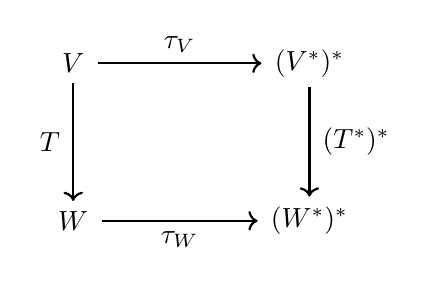
\begin{tikzpicture}[node distance=3cm, auto, thick]
    \node (V) {$V$};
    \node (Vdual) [right of=V] {$(V^*)^*$};
    \node (W) [below of=V, node distance=2cm] {$W$};
    \node (Wdual) [right of=W] {$(W^*)^*$};

    \draw[->] (V) to node {$\tau_V$} (Vdual);
    \draw[->] (V) to node[swap] {$T$} (W);
    \draw[->] (W) to node[swap] {$\tau_W$} (Wdual);
    \draw[->] (Vdual) to node {$(T^*)^*$} (Wdual);
  \end{tikzpicture}
\end{center}

\begin{exercise}
  Let $V$ be a finite-dimensional vector space over $K$, and let $\mathcal{B} = (v_1, \dots, v_n)$ be a basis for $V$. Let $\mathcal{B}^* = (v_1^*, \dots, v_n^*)$ be the dual basis, and let $(\mathcal{B}^*)^* = ((v_1^*)^*, \dots, (v_n^*)^*)$ be the basis for $(V^*)^*$ which is dual to $\mathcal{B}^*$. Show that $\tau(\mathcal{B}) = (\mathcal{B}^*)^*$, meaning $\tau(v_i) = (v_i^*)^*$ for all $1 \leq i \leq n$.
\end{exercise}

\setcounter{section}{1}
\section{Direct Sums}

\subsection{The External Direct Sum}

\begin{proposition}[Vector Space Structure of the Cartesian Product]
  Let $V$ and $W$ be two vector spaces over $K$. Then, the Cartesian product $V \times W$ becomes a vector space over $K$, provided we endow it with the following operations:
  \begin{itemize}
    \item $(v_1, w_1) + (v_2, w_2) := (v_1 + v_2, w_1 + w_2)$ for all $(v_1, w_1), (v_2, w_2) \in V \times W$.
    \item $\alpha \cdot (v, w) := (\alpha v, \alpha w)$ for all $\alpha \in K$ and $(v, w) \in V \times W$.
  \end{itemize}
  The zero element of this space is given by $0_{V \times W} := (0_V, 0_W)$. This new vector space $V \times W$ is usually denoted by $V \oplus W$ and is called the direct sum of $V$ and $W$.
\end{proposition}

\begin{proof}
  Exercise. One must verify that all vector space axioms are satisfied under these componentwise operations.
\end{proof}

\begin{remark}[Canonical Maps associated with Direct Sums]
  The direct sum $V \oplus W$ is naturally equipped with several canonical linear maps:
  \begin{enumerate}
    \item \textbf{Canonical Embeddings}:
    \begin{itemize}
      \item $i_V \colon V \to V \oplus W$ defined by $i_V(v) := (v, 0)$.
      \item $i_W \colon W \to V \oplus W$ defined by $i_W(w) := (0, w)$.
    \end{itemize}
    \item \textbf{Canonical Projections}:
    \begin{itemize}
      \item $p_V \colon V \oplus W \to V$ defined by $p_V(v, w) := v$.
      \item $p_W \colon V \oplus W \to W$ defined by $p_W(v, w) := w$.
    \end{itemize}
  \end{enumerate}
  Clearly, all these maps are linear. Furthermore, the projections $p_V$ and $p_W$ are surjective, while the embeddings $i_V$ and $i_W$ are injective. By virtue of these embeddings, we can often identify $V$ and $W$ as subspaces of $V \oplus W$ through the identifications $v \leftrightarrow (v, 0)$ and $w \leftrightarrow (0, w)$.
\end{remark}

\subsection{Internal Direct Sums and Complements}

\begin{proposition}[Isomorphism to a Complementary Subspace]
  Let $V$ be a vector space over $K$, and let $U \subseteq V$ be a subspace. Suppose $U' \subseteq V$ is another subspace that acts as a complement of $U$ in $V$, which implies that $U + U' = V$ and $U \cap U' = \{0\}$. Then, the map
  \[
  \varphi \colon U \oplus U' \to V, \quad \varphi(u, u') := u + u'
  \]
  is a linear isomorphism.
\end{proposition}

\begin{proof}
  The linearity of $\varphi$ follows immediately from the definitions of the operations in $U \oplus U'$ and the linearity of addition in $V$.

  To establish injectivity, suppose $\varphi(u, u') = 0$, which implies $u + u' = 0$, and therefore $u = -u'$. Since $u \in U$ and $u' \in U'$, it follows that $u = -u' \in U \cap U'$. However, as $U'$ is a complement of $U$, we have $U \cap U' = \{0\}$ by definition. Consequently, $u = u' = 0$, which shows that $\ker(\varphi) = \{0_{U \oplus U'}\}$. Thus, $\varphi$ is injective.

  Regarding surjectivity, we observe that since $U'$ is a complement of $U$ in $V$, we have $U + U' = V$ by definition. Thus, for any $v \in V$, there exist $u \in U$ and $u' \in U'$ such that $u + u' = v$. This implies $\varphi(u, u') = v$, and therefore $\operatorname{Im}(\varphi) = V$. This proves that $\varphi$ is surjective, and consequently, an isomorphism.
\end{proof}

\begin{remark}
  While $U \oplus U'$ is formally a different vector space from $V$, the existence of the canonical isomorphism $\varphi$ allows us to treat $V$ as the direct sum of its internal subspaces whenever a complement is specified.
\end{remark}

Geometrically, in $\mathbb{R}^2$, this represents the decomposition of any vector $v$ uniquely into a sum of a vector $u \in U$ and a vector $u' \in U'$, constructed via a parallelogram parallel to the complementary subspaces:

\begin{center}
  \begin{tikzpicture}[scale=1.2]
    % Axes/Subspaces
    \draw[thick, blue] (-2,-1) -- (3,1.5) node[right] {$U$};
    \draw[thick, red] (-1,2) -- (1.5,-3) node[right] {$U'$};

    % Vectors
    \draw[->, thick, blue!60!black] (0,0) -- (1.6,0.8) node[midway, above left] {$u$};
    \draw[->, thick, red!60!black] (0,0) -- (0.5,-1) node[midway, left] {$u'$};

    % Parallelogram and Resultant
    \draw[dashed, gray] (1.6,0.8) -- (2.1,-0.2);
    \draw[dashed, gray] (0.5,-1) -- (2.1,-0.2);
    \draw[->, very thick, purple] (0,0) -- (2.1,-0.2) node[right] {$v = u + u'$};

    % Origin
    \filldraw (0,0) circle (1.5pt) node[above left] {$0$};
  \end{tikzpicture}
\end{center}

\subsection{Generalization to Multiple Summands}

The concept of a direct sum can be extended to any finite collection of vector spaces $U_1, \dots, U_m$ over $K$. We define their direct sum as:
\[
U_1 \oplus \dots \oplus U_m := U_1 \times \dots \times U_m,
\]
endowed with coordinatewise operations.

For an infinite family of vector spaces $\{U_i\}_{i \in I}$, we define the direct sum $\bigoplus_{i \in I} U_i$ as the set of functions $t \colon I \to \bigcup_{i \in I} U_i$ such that $t(i) \in U_i$ for all $i \in I$, and $t(i) \neq 0$ for at most finitely many indices $i \in I$. This ensures that any element of the direct sum can be represented as a finite formal sum of components.

\setcounter{section}{2}
\section{Quotient Spaces}

\subsection{Equivalence Relation and the Quotient Space}

Let $V$ be a vector space over $K$, and let $U \subseteq V$ be a subspace. We will define a new vector space over $K$, denoted by $V/U$, together with a linear map $\pi \colon V \to V/U$ such that $\pi$ is surjective and $\ker(\pi) = U$.

\begin{definition*}[The Quotient $V/U$ And The Quotient Map $\pi$] The space $V/U$ is called the quotient of $V$ by $U$, or $V$ modulo $U$. The map $\pi$ is called the quotient map, or the projection onto the quotient space.
\end{definition*}

We begin by defining a relation on $V$. For $v_1, v_2 \in V$, we define $v_1 \sim v_2$ if and only if $v_1 - v_2 \in U$.

\begin{lemma*}[Equivalence Relation on $V$]
  The relation $\sim$ defines an equivalence relation on $V$.
\end{lemma*}

\begin{proof}
  Reflexivity: For all $v \in V$, $v \sim v$ because $v - v = 0 \in U$.

  Symmetry: If $v_1 \sim v_2$, then $v_1 - v_2 \in U$. Since $U$ is a subspace, $-(v_1 - v_2) = v_2 - v_1 \in U$, which implies $v_2 \sim v_1$.

  Transitivity: If $v_1 \sim v_2$ and $v_2 \sim v_3$, then $v_1 - v_2 \in U$ and $v_2 - v_3 \in U$. Because $U$ is a subspace, their sum is in $U$:
  \[ (v_1 - v_2) + (v_2 - v_3) = v_1 - v_3 \in U, \]
  which means $v_1 \sim v_3$.
\end{proof}

We denote the equivalence class of $v \in V$ by $[v]$. Thus,
\[ [v] = v + U = \{v + u \mid u \in U\}. \]

\begin{definition}[The Quotient Space]
  Let $V$ be a vector space over $K$, and let $U \subseteq V$ be a subspace. We define the quotient space $V/U$ as the set of equivalence classes of the equivalence relation $\sim$.
\end{definition}

Alternatively, each element in $V/U$ is a set of the form $v + U$, where $v \in V$.

Geometrically, if $V = \mathbb{R}^2$ and $U$ is a line through the origin, the equivalence classes $[v]$ forming the space $V/U$ are precisely the lines parallel to $U$:

\begin{center}
  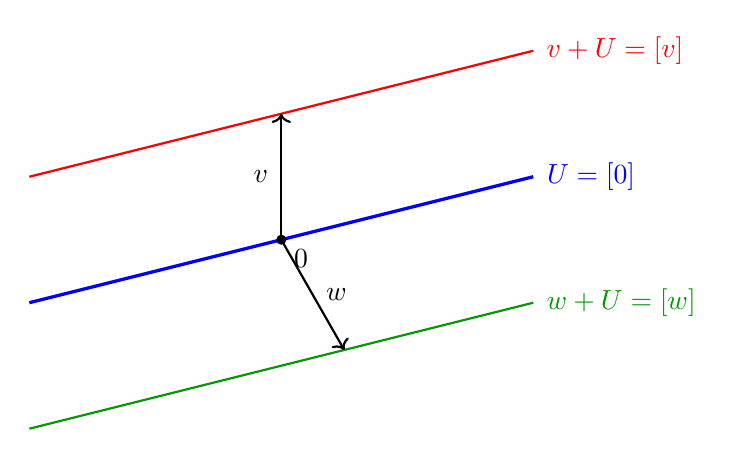
\begin{tikzpicture}[scale=0.8]
    % The subspace U (origin line)
    \draw[very thick, blue] (-4,-1) -- (4,1) node[right] {$U = [0]$};

    % Other equivalence classes (Cosets)
    \draw[thick, red] (-4, 1) -- (4, 3) node[right] {$v + U = [v]$};
    \draw[thick, green!60!black] (-4, -3) -- (4, -1) node[right] {$w + U = [w]$};

    % Vectors defining the shift
    \draw[->, thick] (0,0) -- (0,2) node[midway, left] {$v$};
    \draw[->, thick] (0,0) -- (1,-1.75) node[midway, right] {$w$};

    % Origin
    \filldraw (0,0) circle (2pt) node[below right] {$0$};
  \end{tikzpicture}
\end{center}

\subsection{The Vector Space Structure of $V/U$}

We want to turn $V/U$ into a vector space over $K$. We define addition as $[v_1] + [v_2] := [v_1 + v_2]$ for all $[v_1], [v_2] \in V/U$. Alternatively, this can be written as $(v_1 + U) + (v_2 + U) := (v_1 + v_2) + U$. For scalar multiplication, let $\alpha \in K$ and $[v] \in V/U$. We define $\alpha \cdot [v] := [\alpha v]$. The zero element is defined as $0_{V/U} := [0_V] = U$.

\begin{proposition}[Well-definedness of Operations in $V/U$]
  The operations defined above are well-defined. Moreover, they give $V/U$ the structure of a vector space over $K$.
\end{proposition}

\begin{proof}
  To establish well-definedness, we must show that the operations do not depend on the choice of representatives.
  For scalar multiplication, suppose $[v] = [v']$, and let $\alpha \in K$. We need to show that $[\alpha v] = [\alpha v']$. Indeed, since $[v] = [v']$, we have $v - v' \in U$. Because $U$ is a subspace, $\alpha(v - v') = \alpha v - \alpha v' \in U$. Consequently, $[\alpha v] = [\alpha v']$.

  Similarly, for addition, suppose $[v_1] = [v_1']$ and $[v_2] = [v_2']$. We need to show that $[v_1 + v_2] = [v_1' + v_2']$. By assumption, $v_1 - v_1' \in U$ and $v_2 - v_2' \in U$. Adding these yields:
  \[ (v_1 + v_2) - (v_1' + v_2') = (v_1 - v_1') + (v_2 - v_2') \in U. \]
  Therefore, $v_1 + v_2 \sim v_1' + v_2'$, which implies $[v_1 + v_2] = [v_1' + v_2']$. This proves that the operations are well-defined.

  It remains to show that they satisfy the axioms of a vector space. These follow directly from the corresponding axioms in $V$. (Exercise: complete the proof!)
\end{proof}

We now define a map $\pi \colon V \to V/U$ by $\pi(v) := [v] \in V/U$ for all $v \in V$.

\begin{proposition}[The Quotient Map]
  The map $\pi \colon V \to V/U$ is a linear map. Moreover, it is surjective (i.e., $\operatorname{Im}(\pi) = V/U$), and $\ker(\pi) = U$.
\end{proposition}

\begin{proof}
  Linearity: For $v_1, v_2 \in V$, $\pi(v_1 + v_2) = [v_1 + v_2] = [v_1] + [v_2] = \pi(v_1) + \pi(v_2)$. For $\alpha \in K$ and $v \in V$, $\pi(\alpha v) = [\alpha v] = \alpha [v] = \alpha \pi(v)$.

  Surjectivity: Let $x \in V/U$. By definition, $x$ is an equivalence class $[v]$ of some element $v \in V$. Thus, $x = \pi(v)$.

  Kernel: We claim that $\ker(\pi) = U$. First, let $v \in \ker(\pi)$, meaning $\pi(v) = 0$. Then, $[v] = [0]$, which implies $v = v - 0 \in U$. Hence, $\ker(\pi) \subseteq U$. Conversely, let $u \in U$. Then, $u \sim 0$ because $u - 0 \in U$. Therefore, $\pi(u) = [u] = [0] = 0$, so $u \in \ker(\pi)$. This shows that $U \subseteq \ker(\pi)$, completing the proof.
\end{proof}

\begin{proposition}[Dimension of the Quotient Space]
  Suppose that $V$ is a finite-dimensional vector space. Then, $V/U$ is also finite-dimensional, and $\dim V/U = \dim V - \dim U$.
\end{proposition}

\begin{proof}
  We have seen that $\pi \colon V \to V/U$ is a surjective linear map. This guarantees that $V/U$ is finite-dimensional. (Generally, if $T \colon W' \to W''$ is a surjective linear map and $W'$ is finite-dimensional, then $W''$ is also finite-dimensional, because the images of a basis of $W'$ span $W''$).

  We now apply the Rank-Nullity Theorem to $\pi$:
  \[ \dim V = \dim \ker(\pi) + \dim \operatorname{Im}(\pi). \]
  Since $\ker(\pi) = U$ and $\operatorname{Im}(\pi) = V/U$, we obtain $\dim V/U = \dim V - \dim U$.
\end{proof}

\subsection{The Isomorphism Theorem and Universal Property}

\begin{theorem}[The First Isomorphism Theorem]
  Let $V$ and $W$ be vector spaces over $K$, and let $T \colon V \to W$ be a linear map. We define a new map $\overline{T} \colon V/\ker(T) \to \operatorname{Im}(T)$ as follows: For $x \in V/\ker(T)$, choose a representative $v \in V$ such that $x = [v]$. Define $\overline{T}(x) := T(v)$. Then:
  \begin{enumerate}
    \item $\overline{T}$ is well-defined and is a linear map.
    \item $\overline{T} \colon V/\ker(T) \to \operatorname{Im}(T)$ is an isomorphism.
    \item {The following diagram commutes: $T = i \circ \overline{T} \circ \pi$, where $i \colon \operatorname{Im}(T) \to W$ is the inclusion map.
      \begin{center}
        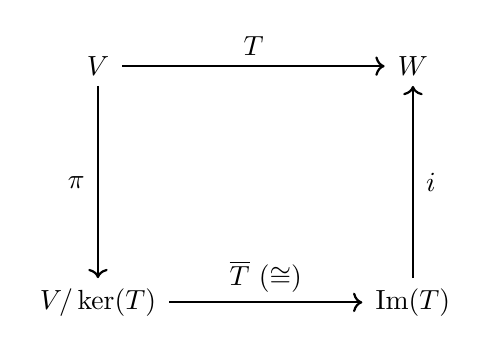
\begin{tikzpicture}[node distance=3cm, auto, thick]
          \node (V) {$V$};
          \node (W) [right of=V, node distance=4cm] {$W$};
          \node (Vmod) [below of=V] {$V/\ker(T)$};
          \node (Im) [below of=W] {$\operatorname{Im}(T)$};

          \draw[->] (V) to node {$T$} (W);
          \draw[->] (V) to node[swap] {$\pi$} (Vmod);
          \draw[->] (Vmod) to node {$\overline{T} \ (\cong)$} (Im);
          \draw[->] (Im) to node[swap] {$i$} (W);
        \end{tikzpicture}
      \end{center}
    }

  \end{enumerate}
\end{theorem}

\begin{proof}
  \begin{enumerate}
    \item To show that $\overline{T}$ is well-defined, suppose $x = [v] = [v']$. We must show that $T(v) = T(v')$. Indeed, $[v] = [v']$ implies that $v - v' \in \ker(T)$, meaning $T(v - v') = 0$. By linearity, $T(v) = T(v')$.

    The linearity of $\overline{T}$ is straightforward: $\overline{T}(\alpha[v]) = \overline{T}([\alpha v]) = T(\alpha v) = \alpha T(v) = \alpha \overline{T}([v])$. Also, $\overline{T}([v_1] + [v_2]) = \overline{T}([v_1 + v_2]) = T(v_1 + v_2) = T(v_1) + T(v_2) = \overline{T}([v_1]) + \overline{T}([v_2])$.

    \item To show that $\overline{T}$ is injective, let $x \in \ker(\overline{T})$, and write $x = [v]$ for some $v \in V$. Then, $\overline{T}(x) = T(v) = 0$, meaning $v \in \ker(T)$. This implies that $x = [v] = 0_{V/\ker(T)}$.

    To show that $\overline{T}$ is surjective, let $w \in \operatorname{Im}(T)$. Then, there exists $v \in V$ such that $T(v) = w$. Consequently, $\overline{T}([v]) = T(v) = w$, proving surjectivity.

    \item The commutativity of the diagram follows immediately from the definitions.
  \end{enumerate}
\end{proof}

\begin{theorem}[Universal Property of Quotient Spaces]
  Let $V$ be a vector space over $K$, and let $U \subseteq V$ be a subspace. The quotient space $V/U$ has the following universal property: For every vector space $W$ and every linear map $T \colon V \to W$ for which $T(U) = 0$ (i.e., for which $\ker(T) \supseteq U$), there exists a unique linear map $T' \colon V/U \to W$ such that $T = T' \circ \pi$. Moreover, $\ker(T') = \ker(T)/U$.
\end{theorem}

\begin{remark}
  In algebraic jargon, every linear map $T \colon V \to W$ that maps $U$ to $0$ factors through $V/U$ via $T = T' \circ \pi$, and moreover, in a unique way. We say that $T$ induces the map $T'$, or that $T$ descends to a map $T' \colon V/U \to W$.
\end{remark}

\begin{proof}
  We define $T' \colon V/U \to W$ as follows: let $x \in V/U$ and choose $v \in V$ such that $x = [v]$. Define $T'(x) := T(v)$. The proof that $T'$ is well-defined and linear follows the exact same logic as in the Isomorphism Theorem. The diagram commutes by construction, since $T'(\pi(v)) = T'([v]) = T(v)$.

  For uniqueness, suppose $T = T'' \circ \pi$ is another factorization. We will show that $T'' = T'$. Let $x \in V/U$. Since $\pi$ is surjective, there exists $v \in V$ such that $x = \pi(v)$. We then have $T(v) = T'(\pi(v))$ and $T(v) = T''(\pi(v))$, which immediately yields $T'(x) = T''(x)$.
\end{proof}

\subsection{Quotients, Complements, and Dual Spaces}

Let $V$ be a vector space over $K$, and let $U \subseteq V$ be a subspace. Let $W \subseteq V$ be a complement of $U$ (i.e., $W$ is a subspace such that $U \cap W = \{0\}$ and $U + W = V$).

\begin{proposition}[Canonical Isomorphism from a Complement]
  Under the assumptions above, there is a canonical isomorphism $Q \colon W \to V/U$, defined by $Q(w) := [w] \in V/U$ for all $w \in W$.
\end{proposition}

\begin{remark}
  The isomorphism $Q$ is canonical only once the complement $W$ is specified. In general, there are many choices of complements to $U$, and there is no preferred choice.
\end{remark}

\begin{proof}
  Consider the inclusion map $i \colon W \to V$ and the projection map $\pi \colon V \to V/U$. Since $Q = \pi \circ i$, $Q$ is a linear map.

  We claim that $\ker(Q) = \{0\}$. Indeed, if $w \in \ker(Q)$, then $[w] = 0$, implying that $w \in U$. However, since $w \in W$, we must have $w \in U \cap W = \{0\}$, and therefore $w = 0$. This shows that $\ker(Q) = \{0\}$.

  We also claim that $Q$ is surjective. Let $x \in V/U$ and choose $v \in V$ such that $x = [v]$. Since $V = U + W$, there exist $u \in U$ and $w \in W$ such that $v = w + u$. It follows that $[v] = [w + u] = [w]$, so $Q(w) = x$. This proves that $Q$ is surjective, and consequently, an isomorphism.
\end{proof}

\subsection{Quotients, Complements, and Annihilators}

\begin{proposition}[Isomorphism from a Specified Complement]
  Let $W \subseteq V$ be a complement of $U$ in $V$. There exists a canonical isomorphism $Q \colon W \to V/U$ defined by $Q(w) := [w]$.
\end{proposition}

\begin{proof}
  $Q$ is the composition of the inclusion $i \colon W \to V$ and the projection $\pi \colon V \to V/U$, and thus is linear. Since $W \cap U = \{0\}$, the kernel of $Q$ is trivial. As $V = U + W$, any $v \in V$ can be written as $w + u$, so $[v] = [w + u] = [w]$, which is $Q(w)$. This proves surjectivity and establishes the isomorphism.
\end{proof}

\begin{proposition}[Annihilators and Dual Quotients]
  Let $U \subseteq V$ be a subspace, and define the annihilator $U^\perp := \{l \in V^* \mid l|_U = 0\}$. Then:
  \begin{enumerate}
    \item $U^\perp \subseteq V^*$ is a linear subspace.
    \item There is a canonical isomorphism $(V/U)^* \cong U^\perp$.
    \item If $V$ is finite-dimensional, then $U^* \cong V^*/U^\perp$.
  \end{enumerate}
\end{proposition}

\begin{proof}
  \begin{enumerate}
    \item Clearly, the zero functional vanishes on $U$. For $l_1, l_2 \in U^\perp$ and $\alpha, \beta \in K$, we have $(\alpha l_1 + \beta l_2)(u) = \alpha l_1(u) + \beta l_2(u) = 0$ for all $u \in U$, establishing that $U^\perp$ is a subspace.

    \item We define a map $L \colon (V/U)^* \to U^\perp$ by $L(s) := s \circ \pi$. This map is well-defined because for any $u \in U$, $(s \circ \pi)(u) = s([u]) = s(0) = 0$. To show linearity, let $s, t \in (V/U)^*$ and $\alpha, \beta \in K$; then
    \[ L(\alpha s + \beta t) = (\alpha s + \beta t) \circ \pi = \alpha(s \circ \pi) + \beta(t \circ \pi) = \alpha L(s) + \beta L(t). \]
    We define an inverse $P \colon U^\perp \to (V/U)^*$ such that for $T \in U^\perp$, $P(T) = T'$, where $T'$ is the unique map induced by the Universal Property of Quotients such that $T = T' \circ \pi$. The identities $L \circ P = \operatorname{id}$ and $P \circ L = \operatorname{id}$ confirm $L$ is a canonical isomorphism.

    \item Assume $V$ is finite-dimensional. Define the restriction map $R \colon V^* \to U^*$ by $R(\varphi) := \varphi|_U$. This map is linear, as $R(\alpha \varphi + \beta \psi) = (\alpha \varphi + \beta \psi)|_U = \alpha R(\varphi) + \beta R(\psi)$. By extending a basis of $U$ to $V$, we can construct a functional on $V$ that matches any functional on $U$, showing $R$ is surjective. Since $\ker(R) = \{\varphi \in V^* \mid \varphi|_U = 0\} = U^\perp$, the First Isomorphism Theorem yields $V^*/U^\perp \cong U^*$.
  \end{enumerate}
\end{proof}

\begin{exercise}
  Let $T \colon V \to W$ be a linear map between vector spaces. Prove that the annihilator of the image of $T$ is equal to the kernel of its dual map:
  \[ (\operatorname{Im} T)^\perp = \ker(T^*). \]
\end{exercise}

\setcounter{chapter}{19} % Chapter 19
\chapter{Miscellaneous Topics and Motivation}

\section{Geometric Motivation: Why Abstraction Matters}

It is a common temptation to simply identify every $n$-dimensional vector space over $K$ with the standard coordinate space $K^n$. However, while they are algebraically isomorphic for any fixed parameter, they may not be "continuously" isomorphic when the vector spaces depend dynamically on parameters.

\subsection{The Möbius Vector Bundle}

\begin{definition}[A Continuous Family of Subspaces]
  Let $S \subseteq \mathbb{C}$ be the unit circle defined by $S = \{e^{i\theta} \mid \theta \in [0, 2\pi]\}$. For each $z = e^{i\theta} \in S$, we define a 1-dimensional subspace $L_z \subseteq \mathbb{R}^2$ as follows:
  \[ L_z := \operatorname{Sp} \left( \cos\frac{\theta}{2}, \sin\frac{\theta}{2} \right). \]
\end{definition}

Notice a topological anomaly: $z=1$ corresponds to both $\theta=0$ and $\theta=2\pi$.
In the first case ($\theta=0$), the spanning vector is $(1,0)$, so $L_1 = \operatorname{Sp}(1,0)$.
In the second case ($\theta=2\pi$), the spanning vector is $(-1,0)$, which gives the exact same subspace $L_1 = \operatorname{Sp}(-1,0)$. The line $L_z$ rotates at exactly half the speed of the point $z$.

\begin{center}
  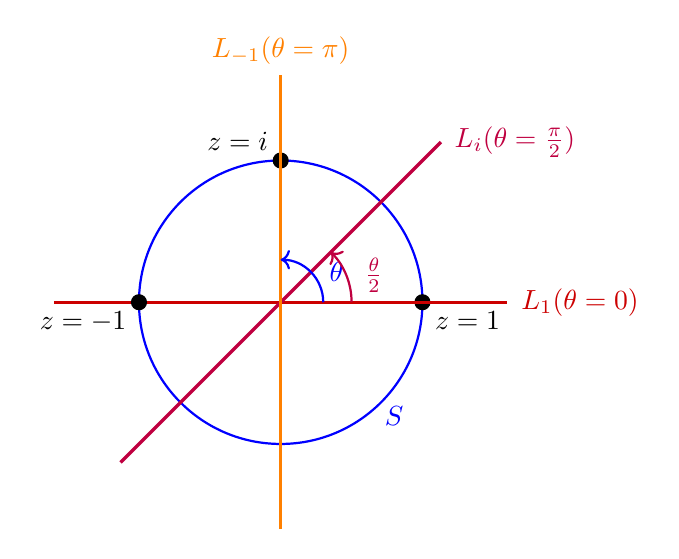
\begin{tikzpicture}[scale=1.8]
    % Background axes
    \draw[gray!40, thin] (-1.5,0) -- (1.5,0);
    \draw[gray!40, thin] (0,-1.5) -- (0,1.5);

    % Unit circle S
    \draw[thick, blue] (0,0) circle (1);
    \node[blue] at (0.8, -0.8) {$S$};

    % theta = 0
    \filldraw[black] (1,0) circle (1.5pt) node[below right] {$z=1$};
    \draw[very thick, red!80!black] (-1.6,0) -- (1.6,0) node[right] {$L_1 (\theta=0)$};

    % theta = pi/2
    \filldraw[black] (0,1) circle (1.5pt) node[above left] {$z=i$};
    \draw[very thick, purple] (-1.13,-1.13) -- (1.13,1.13) node[right] {$L_i (\theta=\frac{\pi}{2})$};

    % theta = pi
    \filldraw[black] (-1,0) circle (1.5pt) node[below left] {$z=-1$};
    \draw[very thick, orange] (0,-1.6) -- (0,1.6) node[above] {$L_{-1} (\theta=\pi)$};

    % Arcs showing the half-speed rotation
    \draw[->, blue, thick] (0.3,0) arc (0:90:0.3) node[midway, right=2pt] {$\theta$};
    \draw[->, purple, thick] (0.5,0) arc (0:45:0.5) node[midway, right=2pt] {$\frac{\theta}{2}$};
  \end{tikzpicture}
\end{center}

\begin{proposition}[Non-triviality of the Möbius Bundle]
  There does not exist a family of linear isomorphisms $T_z \colon L_z \to \mathbb{R}$ that depends continuously on the parameter $z \in S$.
\end{proposition}

\begin{proof}[Proof Sketch]
  Consider the disjoint union of all these lines parameterized by $z$, which forms a space $M = \{ (z, v) \mid z \in S, v \in L_z \}$. Topologically, this forms a vector bundle over $S^1$ known as the Möbius strip.

  If such a continuous family of isomorphisms $T_z$ existed, it would allow us to construct a global homeomorphism $\Phi \colon M \to S \times \mathbb{R}$. Removing the zero-section (the center circle where $v=0$) from both spaces would imply that $M \setminus \{0\} \cong S \times (\mathbb{R} \setminus \{0\})$.

  However, $S \times (\mathbb{R} \setminus \{0\})$ consists of two disconnected cylinders (an "upper" and "lower" half). In contrast, if you cut a Möbius strip down its center line, it remains a single connected piece. This topological contradiction demonstrates that we cannot consistently and continuously identify all $L_z$ with $\mathbb{R}$. Abstraction is therefore necessary to handle "twisted" families of spaces.
\end{proof}

\section{Affine Geometry}

In our strict definition of a vector space, there is always a distinguished origin $0$. Affine geometry studies spaces that "look like" vector spaces locally, but have forgotten their origin.

\begin{definition}[Affine Space]
  A subset $X \subseteq V$ is called an \qt{affine space} if there exists a linear subspace $U \subseteq V$ and a translation vector $x_0 \in V$ such that $X = x_0 + U$.

  We say that $X$ is modeled on the subspace $U$, and we write the \qt{direction space} as $\vec{X} := U$. The elements of $X$ are called \qt{points}, while the elements of $\vec{X}$ are called \qt{vectors}.
\end{definition}

\begin{proposition}[Algebra of Affine Spaces]
  Let $X$ be an affine space modeled on $\vec{X}$. Then:
  \begin{enumerate}
    \item We cannot inherently add two points $p, q \in X$, as $p+q \notin X$ in general.
    \item We can translate a point $p \in X$ by a vector $v \in \vec{X}$ to obtain a new point $p+v \in X$.
    \item For any two points $p, q \in X$, their difference defines a unique vector $\vec{pq} := q - p \in \vec{X}$.
  \end{enumerate}
\end{proposition}

\begin{center}
  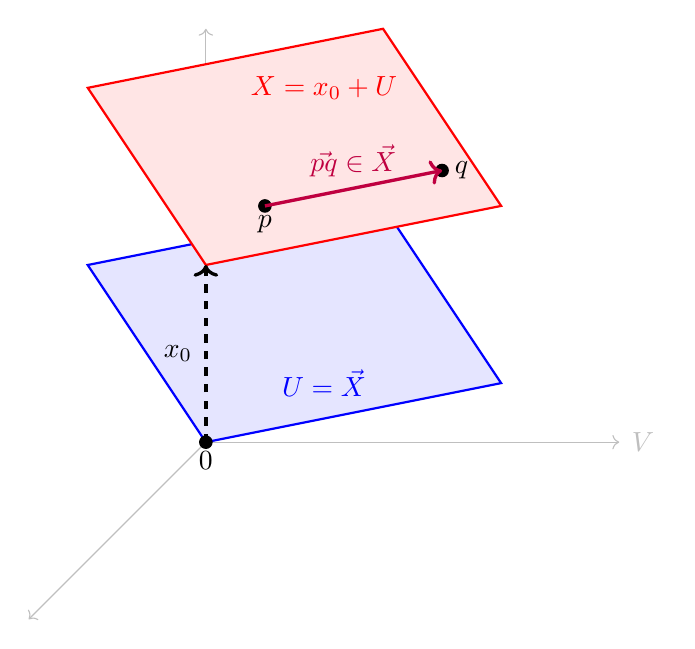
\begin{tikzpicture}[scale=1.5]
    % Axes to imply ambient space V
    \draw[->, gray!50] (0,0) -- (3.5,0) node[right] {$V$};
    \draw[->, gray!50] (0,0) -- (0,3.5);
    \draw[->, gray!50] (0,0) -- (-1.5,-1.5);

    % Subspace U (passing through origin)
    \filldraw[blue!10, draw=blue, thick] (0,0) -- (2.5,0.5) -- (1.5,2) -- (-1,1.5) -- cycle;
    \node[blue] at (1,0.5) {$U = \vec{X}$};

    % Affine space X (displaced)
    \filldraw[red!10, draw=red, thick] (0,1.5) -- (2.5,2.0) -- (1.5,3.5) -- (-1,3.0) -- cycle;
    \node[red] at (1,3) {$X = x_0 + U$};

    % Origin and translation
    \filldraw[black] (0,0) circle (1.5pt) node[below] {$0$};
    \draw[->, very thick, dashed] (0,0) -- (0,1.5) node[midway, left] {$x_0$};

    % Points in X
    \filldraw[black] (0.5, 2.0) circle (1.5pt) node[below] {$p$};
    \filldraw[black] (2.0, 2.3) circle (1.5pt) node[right] {$q$};
    \draw[->, very thick, purple] (0.5, 2.0) -- (2.0, 2.3) node[midway, above] {$\vec{pq} \in \vec{X}$};
  \end{tikzpicture}
\end{center}

\begin{theorem}[Thales' Theorem in Affine Geometry]
  Let $H, H', H''$ be three distinct parallel affine planes in an ambient space $V$. Let $l_1, l_2$ be two affine lines intersecting these planes at the points $p_1, p_1', p_1''$ and $p_2, p_2', p_2''$ respectively. Then:
  \[ \frac{\vec{p_1 p_1''}}{\vec{p_1 p_1'}} = \frac{\vec{p_2 p_2''}}{\vec{p_2 p_2'}}. \]
  Crucially, the ratio of these vectors does not depend on the specific transversals chosen, but only on the relative distances between the parallel planes.
\end{theorem}

\begin{center}
  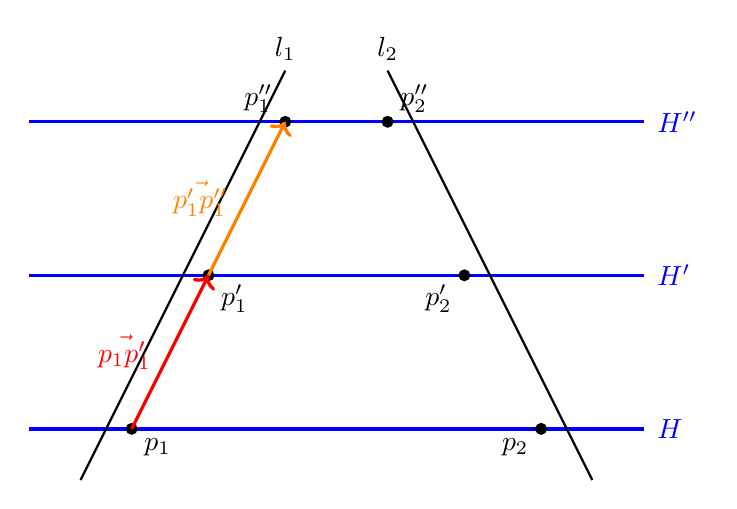
\begin{tikzpicture}[scale=1.3]
    % Parallel planes (represented as lines in 2D projection)
    \draw[very thick, blue] (-1, 3) -- (5, 3) node[right] {$H''$};
    \draw[very thick, blue] (-1, 1.5) -- (5, 1.5) node[right] {$H'$};
    \draw[very thick, blue] (-1, 0) -- (5, 0) node[right] {$H$};

    % Transversal line 1
    \draw[thick, black] (-0.5,-0.5) -- (1.5, 3.5) node[above] {$l_1$};
    \filldraw (0, 0) circle (1.5pt) node[below right] {$p_1$};
    \filldraw (0.75, 1.5) circle (1.5pt) node[below right] {$p_1'$};
    \filldraw (1.5, 3) circle (1.5pt) node[above left] {$p_1''$};

    % Transversal line 2
    \draw[thick, black] (4.5,-0.5) -- (2.5, 3.5) node[above] {$l_2$};
    \filldraw (4, 0) circle (1.5pt) node[below left] {$p_2$};
    \filldraw (3.25, 1.5) circle (1.5pt) node[below left] {$p_2'$};
    \filldraw (2.5, 3) circle (1.5pt) node[above right] {$p_2''$};

    % Vector highlights (corrected)
    \draw[->, very thick, red] (0,0) -- (0.75, 1.5) node[midway, left=2pt] {$\vec{p_1 p_1'}$}; % Vector p1 p1'
    \draw[->, very thick, orange] (0.75, 1.5) -- (1.5, 3) node[midway, left=2pt] {$\vec{p_1' p_1''}$}; % Vector p1' p1''
  \end{tikzpicture}
\end{center}

\section{Introduction to Eigenvalues: Fibonacci Sequences}

\subsection{The Vector Space of Fibonacci Sequences}

Consider the set $Fib \subseteq \mathbb{R}^\infty$ of all infinite real sequences $(a_0, a_1, a_2, \dots)$ that satisfy the linear recurrence relation $a_n = a_{n-1} + a_{n-2}$ for all $n \ge 2$.

\begin{proposition}[Structure of $Fib$]
  The set $Fib$ is a 2-dimensional subspace of $\mathbb{R}^\infty$. The evaluation map $F \colon Fib \to \mathbb{R}^2$ sending a sequence to its first two terms, $(a_n) \mapsto (a_0, a_1)$, is a linear isomorphism.
\end{proposition}

To find a closed-form formula for the Fibonacci numbers (like Binet's formula), we study the \textbf{shift map} $S \colon \mathbb{R}^\infty \to \mathbb{R}^\infty$ defined by shifting the sequence one position to the left:
\[ S(a_0, a_1, a_2, \dots) := (a_1, a_2, a_3, \dots). \]
Since the shifted sequence also satisfies the Fibonacci recurrence, this map restricts to a linear endomorphism $S' \colon Fib \to Fib$.

By utilizing the isomorphism $F$, we can translate the abstract shift operator $S'$ into concrete matrix multiplication on $\mathbb{R}^2$. The sequence $(a_0, a_1)$ shifts to $(a_1, a_2) = (a_1, a_0 + a_1)$, which corresponds to multiplication by the matrix $A = \left(\begin{smallmatrix} 0 & 1 \\ 1 & 1 \end{smallmatrix}\right)$.

\begin{center}
  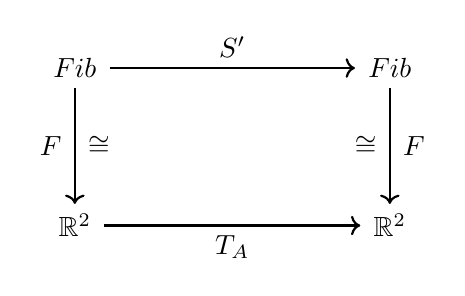
\begin{tikzpicture}[node distance=3cm, auto, thick]
    \node (Fib1) {$Fib$};
    \node (Fib2) [right of=Fib1, node distance=4cm] {$Fib$};
    \node (R1) [below of=Fib1, node distance=2cm] {$\mathbb{R}^2$};
    \node (R2) [below of=Fib2, node distance=2cm] {$\mathbb{R}^2$};

    \draw[->] (Fib1) to node {$S'$} (Fib2);
    \draw[->] (Fib1) to node[swap] {$F$} node {$\cong$} (R1);
    \draw[->] (Fib2) to node {$F$} node[swap] {$\cong$} (R2);
    \draw[->] (R1) to node[swap] {$T_A$} (R2);
  \end{tikzpicture}
\end{center}

\subsection{Eigenvalues and Eigenvectors}

The problem of finding a geometric sequence $(1, \lambda, \lambda^2, \dots)$ inside $Fib$ is equivalent to finding sequences that only scale by $\lambda$ when shifted. That is, we seek vectors $v$ such that $S'(v) = \lambda v$.

\begin{definition}[Eigenvalues and Eigenvectors]
  Let $V$ be a vector space and $T \in \End(V)$. A scalar $\lambda \in K$ is called an \qt{eigenvalue} of $T$ if there exists a non-zero vector $v \in V$ such that:
  \[ T(v) = \lambda v. \]
  The vector $v$ is called an \qt{eigenvector} associated with the eigenvalue $\lambda$.
\end{definition}

In the context of the Fibonacci matrix $A = \left(\begin{smallmatrix} 0 & 1 \\ 1 & 1 \end{smallmatrix}\right)$, calculating the roots of the characteristic polynomial reveals the eigenvalues to be the Golden Ratio $\varphi = \frac{1+\sqrt{5}}{2}$ and its conjugate $\psi = \frac{1-\sqrt{5}}{2}$. Their associated eigenvectors span $Fib$, leading directly to the closed-form Binet formula for the sequence. This forms the primary motivation for the upcoming deeper study of eigenvalues and determinants.
\setcounter{chapter}{19} % Chapter 20
\chapter{Determinants}
\section{Introduction and Motivation}

\subsection{The special case of $2 \times 2$ matrices}
In linear algebra, determining whether a matrix is invertible is a fundamental problem. Let us begin by analyzing the familiar $2 \times 2$ case. Let $A = \left(\begin{smallmatrix} a & b \\ c & d \end{smallmatrix} \right) \in M_{2 \times 2}(K)$. There is a very simple, well-known algebraic criterion to check whether $A$ is invertible.

\begin{proposition}[Invertibility of $2 \times 2$ Matrices]\label{prop:inv_2x2}
  The matrix $A$ is invertible if and only if $ad - bc \neq 0$. Moreover, if $A$ is invertible, then its inverse is given by the explicit formula:
  \[
  A^{-1} = \frac{1}{ad - bc} \begin{pmatrix} d & -b \\ -c & a \end{pmatrix}.
  \]
  The scalar quantity $ad - bc$ is called the determinant of $A$, denoted $\det(A)$.
\end{proposition}

\begin{proof}
  First, we show that $A$ is not invertible if and only if its rank is strictly less than $2$. Because $A$ is a $2 \times 2$ matrix, having a rank less than 2 implies that its column vectors are linearly dependent.

  \begin{remark}[Exercise]\label{rem:lin_dep_2x2_exercise}
    Check that the columns being linearly dependent implies that either the first column is the zero vector (i.e., $\binom{a}{c} = \binom{0}{0}$) or the second column is a scalar multiple of the first (i.e., $\binom{b}{d} = \tau \binom{a}{c}$ for some scalar $\tau \in K$).
  \end{remark}

  If $\binom{a}{c} = \lambda \binom{b}{d}$, then $a = \lambda b$ and $c = \lambda d$. Consequently, $ad - bc = (\lambda b)d - b(\lambda d) = 0$.
  If, on the other hand, $\binom{b}{d} = \tau \binom{a}{c}$, then $b = \tau a$ and $d = \tau c$. Consequently, $ad - bc = a(\tau c) - (\tau a)c = 0$.
  Thus, we have proved that if $A$ is not invertible, then $ad - bc = 0$.

  Conversely, assume $ad - bc = 0$. If $a = 0$, then $bc = 0$, so either $b = 0$ or $c = 0$. This means either $A = \left(\begin{smallmatrix} 0 & 0 \\ c & d \end{smallmatrix}\right)$ or $A = \left(\begin{smallmatrix} 0 & b \\ 0 & d \end{smallmatrix}\right)$. In both of these cases, $A$, clearly, has linearly dependent columns and is therefore not invertible.

  Now, assume $a \neq 0$. This implies $d = \frac{bc}{a}$, and thus we can write $A = \left(\begin{smallmatrix} a & b \\ c & \frac{bc}{a} \end{smallmatrix}\right)$. We can observe that the second column of $A$ is exactly a multiple of the first column because $\binom{b}{\frac{bc}{a}} = \frac{b}{a} \binom{a}{c}$. This implies that the columns of $A$ are linearly dependent. Hence, $\rank(A) < 2$, which implies $A$ is not invertible.
\end{proof}

To confirm the sufficiency of this condition and to find the explicit inverse, the formula for $A^{-1}$ can be verified by direct matrix multiplication:
\[
\frac{1}{ad-bc} \begin{pmatrix} d & -b \\ -c & a \end{pmatrix} \begin{pmatrix} a & b \\ c & d \end{pmatrix} = \frac{1}{ad-bc} \begin{pmatrix} ad-bc & bd-bd \\ -ac+ac & -bc+ad \end{pmatrix} = \begin{pmatrix} 1 & 0 \\ 0 & 1 \end{pmatrix}.
\]

\begin{goals}\label{goals:determinants}
  While the $2 \times 2$ formula is easy to memorize, it does not immediately suggest how to handle larger matrices. Our main goals now are to make the determinant conceptually rigorous and to generalize the determinant function to arbitrary $n \times n$ matrices.
\end{goals}

\subsection{Multilinear and Alternating Functions}

We wish to generalize the determinant to arbitrary dimensions. To this end, we should view an $n \times n$ matrix not just as a grid of numbers, but as a collection of $n$ row vectors.

\begin{definition}[$n$-Linearity]\label{def:n_linear}
  Let $D : M_{n \times n}(K) \to K$ be a function. We say that $D$ is \qt{$n$-linear} if for every $1 \le i \le n$, $D$ is linear as a function of the $i$-th row when all the other $n-1$ rows are held fixed.
\end{definition}

We can think of the matrix space $M_{n \times n}(K)$ as a Cartesian product of row vectors: $K^n_{\text{row}} \times \dots \times K^n_{\text{row}}$. If $A$ has rows $\alpha_1, \dots, \alpha_n$, we write $D(A) = D(\alpha_1, \dots, \alpha_n)$.
Saying that $D$ is $n$-linear means that for any chosen row index $i$, the following two linearity conditions hold:
\begin{enumerate}
  \item $D(\alpha_1, \dots, \alpha_i + \alpha_i', \dots, \alpha_n) = D(\alpha_1, \dots, \alpha_i, \dots, \alpha_n) + D(\alpha_1, \dots, \alpha_i', \dots, \alpha_n)$.
  \item $D(\alpha_1, \dots, c \cdot \alpha_i, \dots, \alpha_n) = c \cdot D(\alpha_1, \dots, \alpha_i, \dots, \alpha_n)$ for all scalars $c \in K$.
\end{enumerate}

\begin{example}\label{ex:n_linear_product}
  For a matrix $A \in M_{n \times n}(K)$, write $A(i,j)$ for its entry at place $i,j$. Let $k_1, \dots, k_n$ be a fixed sequence of integers such that $1 \le k_i \le n$ for all $i$. Fix also a scalar $c \in K$. Consider $D : M_{n \times n}(K) \to K$ defined by the product of one entry from each row:
  \[
  D(A) := c \cdot A(1, k_1) \cdot A(2, k_2) \cdots A(n, k_n).
  \]
  We claim that $D$ is an $n$-linear function.

  To see this, consider $D(\alpha_1, \dots, \alpha_i, \dots, \alpha_n) = b \cdot A(i, k_i)$, where $b \in K$ is the product of all the fixed terms. Notice that $b$ depends only on the rows $\alpha_1, \dots, \alpha_{i-1}, \alpha_{i+1}, \dots, \alpha_n$ and does not depend on row $i$.
  Let $\alpha'_i = (\alpha'_{i,1}, \dots, \alpha'_{i,n})$ be another possible $i$-th row. Then, by standard distribution:
  \[
  D(\dots, \alpha_i + \alpha'_i, \dots) = b \cdot (A(i, k_i) + \alpha'_{i, k_i}) = D(\dots, \alpha_i, \dots) + D(\dots, \alpha'_i, \dots).
  \]
  Similarly, for any scalar $\lambda \in K$:
  \[
  D(\dots, \lambda \cdot \alpha_i, \dots) = b \cdot (\lambda A(i, k_i)) = \lambda \cdot D(\dots, \alpha_i, \dots).
  \]
  Therefore, $D$ is indeed $n$-linear.
\end{example}

\begin{example}[Diagonal Product]\label{ex:diagonal_product}
  A more concrete example: $D(A) := A_{11} \cdot A_{22} \cdot \dots \cdot A_{nn}$ (i.e., the product of the terms on the main diagonal) is an $n$-linear function.
\end{example}

Now let us try to find all 2-linear functions $D: M_{2 \times 2}(K) \to K$. Write the identity matrix as $I = \left(\begin{smallmatrix} -\epsilon_1- \\ -\epsilon_2- \end{smallmatrix}\right)$, where $\epsilon_1 = (1, 0)$ and $\epsilon_2 = (0, 1)$.

If $D$ is 2-linear, then we have:
\begin{align*}
  D(A) &= D(A_{11}\epsilon_1 + A_{12}\epsilon_2, A_{21}\epsilon_1 + A_{22}\epsilon_2) \\
  &= A_{11} D(\epsilon_1, A_{21}\epsilon_1 + A_{22}\epsilon_2) + A_{12} D(\epsilon_2, A_{21}\epsilon_1 + A_{22}\epsilon_2) \\
  &= A_{11}A_{21}D(\epsilon_1, \epsilon_1) + A_{11}A_{22}D(\epsilon_1, \epsilon_2) + A_{12}A_{21}D(\epsilon_2, \epsilon_1) + A_{12}A_{22}D(\epsilon_2, \epsilon_2).
\end{align*}
Therefore, $D$ is completely determined by its values on the following four pairings: $D(\epsilon_1, \epsilon_1)$, $D(\epsilon_1, \epsilon_2)$, $D(\epsilon_2, \epsilon_1)$, and $D(\epsilon_2, \epsilon_2)$.

\begin{lemma}[Closure of $n$-Linear Functions]\label{lem:linear_comb_n_linear}
  Any linear combination of $n$-linear functions is again an $n$-linear function.
\end{lemma}

\begin{proof}
  It is enough to prove this for a linear combination of two $n$-linear functions. Let $D, E : M_{n \times n}(K) \to K$ be $n$-linear functions and $a, b \in K$. We define the combined function as $(aD + bE)(A) := aD(A) + bE(A)$.
  By expanding $(aD+bE)(\dots, \alpha_i + \alpha'_i, \dots)$ and $(aD+bE)(\dots, \lambda \alpha_i, \dots)$ using the individual linearities of $D$ and $E$, we see the result naturally holds.
\end{proof}

\begin{example}\label{ex:2_linear_det}
  Consider $D : M_{2 \times 2}(K) \to K$ defined by $D(A) := A_{11}A_{22} - A_{12}A_{21}$. The function $D$ is $2$-linear because it can be written as $D = D_1 + D_2$, where $D_1(A) = A_{11}A_{22}$ and $D_2(A) = -A_{12}A_{21}$, both of which are 2-linear by our previous example. Furthermore, $D(I) = 1$, and if $A'$ is obtained from $A$ by interchanging the rows, then $D(A') = -D(A)$.

  Indeed, $D(A') = D\left(\begin{smallmatrix} A_{21} & A_{22} \\ A_{11} & A_{12} \end{smallmatrix}\right) = A_{21} \cdot A_{12} - A_{22}A_{11} = -(A_{11}A_{22} - A_{12}A_{21}) = -D(A)$.
\end{example}

\begin{definition}[Alternating Property]\label{def:alternating}
  Let $D : M_{n \times n}(K) \to K$ be an $n$-linear function. We say that $D$ is \qt{alternating} if for every matrix $A$ in which some two rows are equal, we have $D(A) = 0$.
\end{definition}

\begin{proposition}[Adjacent Swap Property]\label{prop:alternating_swap}
  Let $D$ be an $n$-linear function. Assume that $D$ has the property that whenever $A$ has two equal adjacent rows, then $D(A) = 0$. Then the following are equivalent:
  \begin{enumerate}
    \item $D$ is alternating.
    \item For any matrix $B$, if $B'$ is obtained from $B$ by interchanging two of its rows, then $D(B') = -D(B)$.
  \end{enumerate}
\end{proposition}

\begin{proof}
  We begin with the proof of \textbf{(b)}. Assume first that $B'$ is obtained from $B$ by interchanging two adjacent rows (say, row $k$ and row $k+1$).
  Consider evaluating $D$ on a matrix where both the $k$-th and $(k+1)$-th rows are equal to $\beta_k + \beta_{k+1}$. By our assumption, this yields $0$.
  Expanding this via $n$-linearity gives:
  \[
  D(\dots, \beta_k + \beta_{k+1}, \beta_k + \beta_{k+1}, \dots) = D(\dots, \beta_k, \beta_k, \dots) + D(\dots, \beta_k, \beta_{k+1}, \dots)
  \]
  \[
  + D(\dots, \beta_{k+1}, \beta_k, \dots) + D(\dots, \beta_{k+1}, \beta_{k+1}, \dots) = 0.
  \]
  By assumption, the terms with adjacent equal rows are zero, leaving $D(B) + D(B') = 0$, which naturally implies $D(B') = -D(B)$.

  Now suppose $B'$ is obtained from $B$ by interchanging rows $k$ and $\ell$ where $k < \ell$. We can obtain $B'$ by doing a sequence of adjacent row interchanges. Moving row $\ell$ to position $k$ requires $r = \ell-k$ adjacent interchanges. Next, moving the original row $k$ down to position $\ell$ requires $r-1$ adjacent interchanges. The total number of interchanges is $2r - 1$. Since this is always an odd number, we flip the sign an odd number of times. Thus, $D(B') = (-1)^{2r-1} D(B) = -D(B)$.

  We now prove \textbf{(a)}. Let $A$ be a matrix in which row $i$ equals row $j$ where $i < j$. If $j = i+1$, then by assumption $D(A) = 0$. If $j > i+1$, we interchange row $j$ with row $i+1$ to obtain a matrix $A'$ with two equal adjacent rows.
  By assumption $D(A') = 0$, but by \textbf{(b)}, $D(A') = -D(A)$, which implies $D(A) = 0$.
\end{proof}

\subsection{The Determinant Function}

\begin{definition}[Determinant Function]\label{def:determinant_func}
  A function $D : M_{n \times n}(K) \to K$ is called a \qt{determinant function} if it is $n$-linear, it is alternating, and it normalizes the identity matrix such that $D(I) = 1$.
\end{definition}

\begin{example}[Warmup]
  Let us find all determinant functions on $M_{2 \times 2}(K)$. Write $I = \left(\begin{smallmatrix} 1 & 0 \\ 0 & 1 \end{smallmatrix}\right) = \left(\begin{smallmatrix} -\epsilon_1- \\ -\epsilon_2- \end{smallmatrix}\right)$, meaning $\epsilon_1 = (1,0)$ and $\epsilon_2 = (0,1)$.
  If $D$ is a $2$-linear function, we can expand it algebraically:
  \begin{align*}
    D(A) &= D(A_{11}\epsilon_1 + A_{12}\epsilon_2, A_{21}\epsilon_1 + A_{22}\epsilon_2) \\
    &= A_{11} D(\epsilon_1, A_{21}\epsilon_1 + A_{22}\epsilon_2) + A_{12} D(\epsilon_2, A_{21}\epsilon_1 + A_{22}\epsilon_2) \\
    &= A_{11}A_{21}D(\epsilon_1, \epsilon_1) + A_{11}A_{22}D(\epsilon_1, \epsilon_2) \\
    &\quad + A_{12}A_{21}D(\epsilon_2, \epsilon_1) + A_{12}A_{22}D(\epsilon_2, \epsilon_2).
  \end{align*}
  Consequently, $D$ is completely determined by its values on these standard basis row pairings.

  If $D$ is alternating, then evaluating equal rows gives zero, meaning $D(\epsilon_1, \epsilon_1) = D(\epsilon_2, \epsilon_2) = 0$. Additionally, swapping rows flips the sign, so $D(\epsilon_2, \epsilon_1) = -D(\epsilon_1, \epsilon_2) = -D(I)$.
  Finally, if $D$ is a determinant function, $D(I) = 1$. Substituting these values back into our expansion, we perfectly recover the familiar formula:
  \[
  D(A) = A_{11}A_{22}(1) + A_{12}A_{21}(-1) = A_{11}A_{22} - A_{12}A_{21}.
  \]
  Therefore, the $2 \times 2$ determinant function is completely unique!
\end{example}

\begin{definition}[Submatrix]\label{def:minor_submatrix}
  Let $A \in M_{n \times n}(K)$, $n \ge 2$, and $1 \le i \le n$, $1 \le j \le n$. We denote by $A(i|j) \in M_{(n-1) \times (n-1)}(K)$ the \qt{submatrix} obtained from $A$ by deleting row $i$ and column $j$. If $D$ is an $(n-1)$-linear function, we intuitively define $D_{ij}(A) := D(A(i|j))$.
\end{definition}

\begin{theorem}[Recursive Construction of Determinants]\label{thm:recursive_det}
  Let $n \ge 2$, and let $D$ be an $(n-1)$-linear function which is alternating. Let $1 \le j \le n$. Define $E_j : M_{n \times n}(K) \to K$ by
  \[
  E_j(A) := \sum_{i=1}^n (-1)^{i+j} A_{ij} D_{ij}(A).
  \]
  Then, $E_j$ is an $n$-linear function and it is alternating. Furthermore, if $D$ is a determinant function, then so is $E_j$.
\end{theorem}

\begin{proof}
  Clearly, $D_{ij}(A)$ is independent of the $i$-th row of $A$ because that row is deleted in the construction of $A(i|j)$. Since $D$ is $(n-1)$-linear, the map $A \mapsto D_{ij}(A)$ is linear when viewed as a function of each of its remaining rows. The function $A \mapsto A_{ij} D_{ij}(A)$ is therefore $n$-linear. Since linear combinations of $n$-linear functions are $n$-linear, $E_j(A)$ is $n$-linear too.

  We show that $E_j$ is alternating. By Proposition~\ref{prop:alternating_swap}, it is enough to show $E_j(A) = 0$ whenever $A$ has two equal adjacent rows.
  Assume $\alpha_k = \alpha_{k+1}$ for some index $k$. For any $i \neq k, k+1$, the submatrix $A(i|j)$ still has two equal rows, hence $D_{ij}(A) = 0$. This leaves only two non-zero terms in the sum:
  \[
  E_j(A) = (-1)^{k+j} A_{kj} D_{kj}(A) + (-1)^{k+1+j} A_{(k+1)j} D_{(k+1)j}(A).
  \]
  But, since $\alpha_k = \alpha_{k+1}$, we have $A_{kj} = A_{(k+1)j}$ and $A(k|j) = A(k+1|j)$, meaning $D_{kj}(A) = D_{(k+1)j}(A)$. Thus, the two terms perfectly cancel out, yielding $E_j(A) = 0$. This proves $E_j$ is alternating.

  Finally, assume $D$ is a determinant function, meaning $D(I_{n-1}) = 1$. Note that $I_n(j|j) = I_{n-1}$ for all $j$. When computing $E_j(I_n)$, the term $(I_n)_{ij}$ is $1$ if $i=j$, and $0$ if $i \neq j$. Therefore, the sum collapses to a single term:
  \[
  E_j(I_n) = (-1)^{j+j} D_{jj}(I_n) = D(I_n(j|j)) = 1.
  \]
  This shows that $E_j$ is a valid determinant function.
\end{proof}

\begin{corollary}[Existence of Determinants]\label{cor:det_exists}
  For all $n \ge 1$, at least one determinant function exists.
\end{corollary}

\begin{example}
  Consider $A \in M_{3 \times 3}(K)$. Using the uniquely defined $2 \times 2$ determinant function $|B| := B_{11}B_{22} - B_{12}B_{21}$, we can explicitly write out $E_1(A)$ as:
  \[
  E_1(A) = A_{11} \begin{vmatrix} A_{22} & A_{23} \\ A_{32} & A_{33} \end{vmatrix} - A_{21} \begin{vmatrix} A_{12} & A_{13} \\ A_{32} & A_{33} \end{vmatrix} + A_{31} \begin{vmatrix} A_{12} & A_{13} \\ A_{22} & A_{23} \end{vmatrix}.
  \]
  We can similarly construct $E_2(A)$ and $E_3(A)$ along the other columns, and all of these form valid determinant functions on $M_{3 \times 3}(K)$.
\end{example}

\section{Uniqueness of the Determinant}

We have shown that a determinant function exists. Now, we will prove that it is absolutely unique. Let $D : M_{n \times n}(K) \to K$ be an $n$-linear alternating function.
Let $A \in M_{n \times n}(K)$ be a matrix with rows $\alpha_1, \dots, \alpha_n$. We denote the identity matrix as $I$, whose rows are the standard basis vectors $\epsilon_1, \dots, \epsilon_n$ of $K^n_{\text{row}}$.

Clearly, we can express each row of $A$ in terms of the standard basis: $\alpha_i = \sum_{j=1}^n A(i,j)\epsilon_j$ for $1 \le i \le n$. Using the $n$-linearity of $D$, we can expand $D(A)$ as follows:
\begin{align*}
  D(A) &= D(\alpha_1, \dots, \alpha_n) \\
  &= D\left(\sum_{j=1}^n A(1,j)\epsilon_j, \alpha_2, \dots, \alpha_n\right) \\
  &= \sum_{j=1}^n A(1,j) \cdot D(\epsilon_j, \alpha_2, \dots, \alpha_n) \\
  &= \sum_{j=1}^n A(1,j) \cdot D\left(\epsilon_j, \sum_{k=1}^n A(2,k)\epsilon_k, \dots, \alpha_n\right) \\
  &= \sum_{j,k} A(1,j) \cdot A(2,k) \cdot D(\epsilon_j, \epsilon_k, \dots, \alpha_n)
\end{align*}
where both $j$ and $k$ run between $1$ and $n$. Continuing this expansion for all $n$ rows yields an enormous sum:
\[
D(A) = \sum_{k_1, \dots, k_n} A(1,k_1) \cdot A(2,k_2) \cdots A(n,k_n) \cdot D(\epsilon_{k_1}, \epsilon_{k_2}, \dots, \epsilon_{k_n})
\]
where each of the indices $k_1, \dots, k_n$ runs between $1$ and $n$.

Thus far, we have not used the fact that $D$ is alternating. Because $D$ is alternating, the term $D(\epsilon_{k_1}, \dots, \epsilon_{k_n}) = 0$ whenever two of the indices $k_1, \dots, k_n$ are equal. Thus, we are interested only in ordered sequences $(k_1, \dots, k_n)$ in which $k_i \in \{1, \dots, n\}$ for all $i$, and $k_i \neq k_j$ for all $i \neq j$.

Such a sequence is called a \qt{permutation} of $\{1, \dots, n\}$, or a permutation of degree $n$. Alternatively, we can think of a permutation of degree $n$ as a bijective function $\sigma : \{1, \dots, n\} \to \{1, \dots, n\}$. Then, the sequence $(k_1, \dots, k_n) = (\sigma(1), \sigma(2), \dots, \sigma(n))$ is a permutation as defined earlier. In other words, a permutation of degree $n$ is simply a re-ordering of a list of $n$ elements: $(1, \dots, n) \mapsto (\sigma(1), \dots, \sigma(n))$.

We can nicely rewrite our expansion of $D(A)$ as:
\[
D(A) = \sum_{\sigma} A(1,\sigma(1)) \cdot A(2,\sigma(2)) \cdots A(n,\sigma(n)) \cdot D(\epsilon_{\sigma(1)}, \epsilon_{\sigma(2)}, \dots, \epsilon_{\sigma(n)})
\]
where $\sigma$ runs over all possible permutations of degree $n$.

\subsection{Properties of Permutations}

An important property about permutations is that if $\sigma$ is a permutation of degree $n$, one can pass from the sequence $(1, \dots, n)$ to $(\sigma(1), \dots, \sigma(n))$ by performing a finite sequence of interchanges of pairs.

More precisely, a \qt{transposition} is a permutation $\theta : \{1, \dots, n\} \to \{1, \dots, n\}$ for which there exist $i, j \in \{1, \dots, n\}$ with $i \neq j$ such that $\theta(i) = j$, $\theta(j) = i$, and $\theta(k) = k$ for all $k \neq i,j$.

Every permutation $\sigma$ can be written as a composition of transpositions:
\begin{equation} \label{eq:permutation_decomp}
  \sigma = \theta_1 \circ \cdots \circ \theta_m
\end{equation}
where $\theta_1, \dots, \theta_m$ are transpositions. However, these $\theta_i$'s and the total number $m$ are not unique. The same permutation $\sigma$ can be written as $\sigma = \theta_1 \circ \cdots \circ \theta_m = \theta'_1 \circ \cdots \circ \theta'_{m'}$.

\begin{remark}
  Why is the decomposition \eqref{eq:permutation_decomp} always possible? Start with the sorted list $(1, \dots, n)$. If $\sigma(1) \neq 1$, then interchange $1$ and $\sigma(1)$. We now have $(\sigma(1), \dots, 1, \dots, n)$. Next, look at the second position. If it is not $\sigma(2)$, interchange it with $\sigma(2)$, and proceed similarly down the line. Of course, there are other ways to do it. For example, the permutation $(3,2,1)$ can be obtained in 3 steps:
  \[ (1,2,3) \to (2,1,3) \to (2,3,1) \to (3,2,1) \]
  But, it can also be obtained in just one step: $(1,2,3) \to (3,2,1)$.
\end{remark}

\begin{lemma}[Parity of Transpositions]\label{lem:permutation_parity}
  If $(\sigma(1), \dots, \sigma(n))$ is obtained from $(1, \dots, n)$ in two different ways—one time by a sequence of $m$ transpositions, and another time by a sequence of $m'$ transpositions—then $m$ and $m'$ must have the same parity. That is, $m'$ is even if and only if $m$ is even, and $m'$ is odd if and only if $m$ is odd.
\end{lemma}

In other words, $(-1)^{m'} = (-1)^m$. The parity depends only on the permutation $\sigma$, and not on the particular sequence of transpositions used.

A permutation $\sigma$ is called \qt{even} if $m$ is even, and \qt{odd} if $m$ is odd. The number $\operatorname{sgn}(\sigma) := (-1)^m \in \{-1, 1\}$ is called the \qt{sign} of $\sigma$.

\begin{proof}[Proof of Lemma]
  We know from previous results that determinant functions $E : M_{n \times n}(K) \to K$ exist for $n \ge 1$. Let us fix one such determinant function $E$ (we denote it by $E$ to distinguish it from $D$ in the previous discussion).

  Consider the evaluation $E(\epsilon_{\sigma(1)}, \dots, \epsilon_{\sigma(n)})$. If $(\sigma(1), \dots, \sigma(n))$ can be obtained from $(1, \dots, n)$ by a sequence of $m$ transpositions, then the matrix with rows $\epsilon_{\sigma(1)}, \dots, \epsilon_{\sigma(n)}$ can be obtained from the identity matrix $I$ by a sequence of $m$ interchanges of pairs of rows.

  Because $E$ is alternating, swapping two rows flips the sign of the output. Therefore:
  \[
  E(\epsilon_{\sigma(1)}, \dots, \epsilon_{\sigma(n)}) = (-1)^m E(\epsilon_1, \dots, \epsilon_n) = (-1)^m E(I) = (-1)^m.
  \]
  But, this exact same logic applies to the sequence of $m'$ transpositions. Thus:
  \[
  E(\epsilon_{\sigma(1)}, \dots, \epsilon_{\sigma(n)}) = (-1)^{m'} E(\epsilon_1, \dots, \epsilon_n) = (-1)^{m'} E(I) = (-1)^{m'}.
  \]
  This identically implies that $(-1)^m = (-1)^{m'}$, proving the lemma.
\end{proof}

Returning to our original function $D(A)$, we have seen that:
\[
D(A) = \sum_{\sigma} A(1,\sigma(1)) \cdots A(n,\sigma(n)) \cdot D(\epsilon_{\sigma(1)}, \dots, \epsilon_{\sigma(n)}).
\]
By the alternating property of $D$, performing the transpositions necessary to sort $(\sigma(1), \dots, \sigma(n))$ back to $(1, \dots, n)$ yields:
\begin{equation} \label{eq:det_relation}
  D(\epsilon_{\sigma(1)}, \dots, \epsilon_{\sigma(n)}) = \operatorname{sgn}(\sigma) \cdot D(\epsilon_1, \dots, \epsilon_n) = \operatorname{sgn}(\sigma) \cdot D(I).
\end{equation}

\begin{theorem}[Leibniz Formula \& Uniqueness]
  \label{thm:unique_det}
  For all $n \ge 1$, there exists a unique determinant function on $M_{n \times n}(K)$. We will denote it by $\det$. It is mathematically given by the formula:
  \[
  \det(A) = \sum_{\sigma} \operatorname{sgn}(\sigma) \cdot A(1,\sigma(1)) \cdot A(2,\sigma(2)) \cdots A(n,\sigma(n)).
  \]
\end{theorem}

\begin{proof}
  This follows immediately from \eqref{eq:det_relation}. Indeed, if $D$ is a determinant function, then $D(I) = 1$. Substituting this into \eqref{eq:det_relation} yields the exact formula for $D(A)$ stated in the theorem, proving that the function is entirely unique.
\end{proof}

\begin{corollary}[Scaling of Alternating Functions]
  \label{cor:det_pullout}
  For any $n$-linear alternating function $D : M_{n \times n}(K) \to K$, we have $D(A) = \det(A) \cdot D(I)$ for all $A \in M_{n \times n}(K)$.
\end{corollary}

\subsection{The Symmetric Group}

Denote by $S_n$ the set of permutations $\sigma : \{1, \dots, n\} \to \{1, \dots, n\}$. The set $S_n$ has the algebraic structure of a group under composition: if $\sigma, \tau \in S_n$, their composition is $(\sigma \circ \tau)(x) = \sigma(\tau(x))$. The identity function $\operatorname{id}$ is the neutral element. The inverse $\sigma^{-1}$ exists because $\sigma$ is bijective. Furthermore, the size of the symmetric group is $|S_n| = n!$ (Exercise).

\begin{lemma}[Multiplicativity of Signum]
  \label{lem:sgn_multiplicative}
  For all $\sigma, \tau \in S_n$, we have $\operatorname{sgn}(\sigma \circ \tau) = \operatorname{sgn}(\sigma) \cdot \operatorname{sgn}(\tau)$.
\end{lemma}

\begin{proof}
  Suppose $\sigma = \theta_1 \circ \cdots \circ \theta_m$ and $\tau = \lambda_1 \circ \cdots \circ \lambda_{\ell}$, where the $\theta_i$'s and $\lambda_j$'s are all transpositions. Then, their composition is simply $\sigma \circ \tau = \theta_1 \circ \cdots \circ \theta_m \circ \lambda_1 \circ \cdots \circ \lambda_{\ell}$, which explicitly consists of $m + \ell$ transpositions. Therefore:
  \[
  \operatorname{sgn}(\sigma \circ \tau) = (-1)^{m+\ell} = (-1)^m \cdot (-1)^{\ell} = \operatorname{sgn}(\sigma) \cdot \operatorname{sgn}(\tau).
  \]
\end{proof}

\subsection{Multiplicativity of the Determinant}

\begin{theorem}[Multiplicativity of the Determinant]
  \label{thm:det_multiplicative}
  For any matrices $A, B \in M_{n \times n}(K)$, we have $\det(A \cdot B) = \det(A) \cdot \det(B)$.
\end{theorem}

\begin{proof}
  Fix a matrix $B \in M_{n \times n}(K)$, and consider a function $D : M_{n \times n}(K) \to K$ defined by $D(A) := \det(A \cdot B)$.

  Claim: $D$ is $n$-linear and alternating.

  Proof of claim: Let the rows of $A$ be $\alpha_1, \dots, \alpha_n$. If we view $\alpha_i$ as a $1 \times n$ matrix, then the matrix product $\alpha_i \cdot B$ is also $1 \times n$. In fact, the rows of the product matrix $A \cdot B$ are exactly $\alpha_1 \cdot B, \dots, \alpha_n \cdot B$. So, $D(A) = \det(\alpha_1 \cdot B, \dots, \alpha_n \cdot B)$.

  Clearly, for two row vectors $\alpha_i$ and $\alpha'_i$, we have $(\alpha_i + \alpha'_i) \cdot B = \alpha_i \cdot B + \alpha'_i \cdot B$. Also, for any scalar $c \in K$, $(c\alpha_i) \cdot B = c(\alpha_i \cdot B)$. Since the determinant function $\det$ is $n$-linear with respect to its rows, it heavily follows that $D$ is also $n$-linear.

  Furthermore, if two rows of $A$ are equal (i.e., $\alpha_i = \alpha_j$), then the corresponding rows of $A \cdot B$ are also equal ($\alpha_i \cdot B = \alpha_j \cdot B$). Because $\det$ is alternating, $D(A) = \det(\alpha_1 \cdot B, \dots, \alpha_n \cdot B) = 0$. This rigorously proves the claim that $D$ is alternating.

  We continue with the proof of Theorem~\ref{thm:det_multiplicative}. By Corollary~\ref{cor:det_pullout}, any $n$-linear alternating function satisfies $D(A) = \det(A) \cdot D(I)$. We compute $D(I)$ using our definition: $D(I) = \det(I \cdot B) = \det(B)$. Substituting this back yields $D(A) = \det(A) \cdot \det(B)$, completing the proof.
\end{proof}

\begin{corollary}[Determinant of an Inverse]
  \label{cor:det_inverse}
  If $A$ is invertible, then $\det(A) \neq 0$. Moreover, $\det(A^{-1}) = \frac{1}{\det(A)}$.
\end{corollary}

\begin{proof}
  Assume $A$ is invertible, and denote its inverse by $A^{-1}$. Since $A \cdot A^{-1} = I$, taking the determinant of both sides and applying Theorem~\ref{thm:det_multiplicative} yields $\det(A) \cdot \det(A^{-1}) = \det(I) = 1$. This automatically implies that $\det(A)$ cannot be zero, and dividing by $\det(A)$ yields the expected formula.
\end{proof}

\section{More on Determinants: Properties of Determinants and the Transpose}

Recall that for any matrix $M \in M_{m \times n}(K)$, we have the transposed matrix $M^T \in M_{n \times m}(K)$, where the entries are given by $M^T(i,j) = M(j,i)$.

\begin{theorem}[Determinant of the Transpose]
  \label{thm:det_transpose}
  For all $A \in M_{n \times n}(K)$, we have $\det(A^T) = \det(A)$.
\end{theorem}

\begin{proof}
  If $\sigma$ is a permutation of degree $n$, then by definition of the transpose, $A^T(i, \sigma(i)) = A(\sigma(i), i)$.
  Therefore, expanding the determinant definition gives:
  \[
  \det(A^T) = \sum_{\sigma \in S_n} \operatorname{sgn}(\sigma) \cdot A(\sigma(1), 1) \cdots A(\sigma(n), n).
  \]
  If we let $j = \sigma(i)$, then $i = \sigma^{-1}(j)$, and consequently $A(\sigma(i), i) = A(j, \sigma^{-1}(j))$. Hence, we can rearrange the product completely:
  \begin{equation} \label{eq:transpose_prod}
    A(\sigma(1), 1) \cdots A(\sigma(n), n) = A(1, \sigma^{-1}(1)) \cdots A(n, \sigma^{-1}(n))
  \end{equation}
  This holds because every factor on the left-hand side of \eqref{eq:transpose_prod} will appear exactly once on the right-hand side, and vice-versa.

  Now, since $\sigma \circ \sigma^{-1} = \operatorname{id}$, we have $\operatorname{sgn}(\sigma) \cdot \operatorname{sgn}(\sigma^{-1}) = \operatorname{sgn}(\operatorname{id}) = 1$, which implies $\operatorname{sgn}(\sigma) = \operatorname{sgn}(\sigma^{-1})$.
  When $\sigma$ runs over $S_n$ (all possible permutations of degree $n$), its inverse $\sigma^{-1}$ also naturally runs over the entirety of $S_n$.

  This implies:
  \begin{align*}
    \det(A^T) &= \sum_{\sigma \in S_n} \operatorname{sgn}(\sigma) A(\sigma(1), 1) \cdots A(\sigma(n), n) \\
    &= \sum_{\sigma \in S_n} \operatorname{sgn}(\sigma^{-1}) A(1, \sigma^{-1}(1)) \cdots A(n, \sigma^{-1}(n)) \\
    &= \sum_{\tau \in S_n} \operatorname{sgn}(\tau) A(1, \tau(1)) \cdots A(n, \tau(n)) \\
    &= \det(A).
  \end{align*}
\end{proof}

\begin{example}
  Let $A = \left(\begin{smallmatrix} 1 & 2 \\ 3 & 4 \end{smallmatrix}\right)$. Its transpose is $A^T = \left(\begin{smallmatrix} 1 & 3 \\ 2 & 4 \end{smallmatrix}\right)$. We have $\det(A) = (1)(4) - (2)(3) = -2$, and $\det(A^T) = (1)(4) - (3)(2) = -2$. Thus, the theorem holds.
\end{example}

\begin{corollary}[Column Alternating Property]
  \label{cor:det_columns}
  If $D : M_{n \times n}(K) \to K$ is an alternating $n$-linear function of the rows of the matrix, then $D$ is also an alternating $n$-linear function of the columns of the matrix. In fact, $D(A^T) = D(A)$ for all $A \in M_{n \times n}(K)$. In particular, this holds for $D = \det$.
\end{corollary}

\begin{proof}
  For any $A \in M_{n \times n}(K)$, we have previously established $D(A) = \det(A) \cdot D(I)$. Applying this to $A^T$ gives $D(A^T) = \det(A^T) \cdot D(I)$. Since $\det(A^T) = \det(A)$, this evaluates exactly to $\det(A) \cdot D(I) = D(A)$.
\end{proof}

Because the determinant acts symmetrically on rows and columns, we can perform column operations just as we do row operations.

\begin{theorem}[Invariance Under Row Operations]
  \label{thm:row_operations}
  Let $A \in M_{n \times n}(K)$.
  \begin{enumerate}
    \item If $B$ is obtained from $A$ by adding a multiple of one row of $A$ to another row (i.e., $R_i + c R_j \to R_i$ for $i \neq j$), or by doing the analogous operation on columns, then $\det(B) = \det(A)$.
    \item If $B$ is obtained from $A$ by interchanging two rows (i.e., $R_i \leftrightarrow R_j$ for $i \neq j$), or columns, then $\det(B) = -\det(A)$.
    \item If $B$ is obtained from $A$ by multiplying a row by a scalar (i.e., $c R_i \to R_i$), then $\det(B) = c \det(A)$.
  \end{enumerate}
\end{theorem}

\begin{proof}
  Statement \textbf{(b)} follows directly from the fact that the determinant is an alternating function. Statement \textbf{(c)} follows from the $n$-linearity of the determinant.

  To prove \textbf{(a)}, let $A$ have rows $\alpha_1, \dots, \alpha_n$. Assume $j < i$. Expanding by linearity on the $i$-th row gives:
  \begin{align*}
    \det(B) &= \det(\alpha_1, \dots, \alpha_i + c\alpha_j, \dots, \alpha_j, \dots, \alpha_n) \\
    &= \det(\alpha_1, \dots, \alpha_i, \dots, \alpha_n) + c \det(\alpha_1, \dots, \alpha_j, \dots, \alpha_j, \dots, \alpha_n) \\
    &= \det(A) + 0 = \det(A).
  \end{align*}
  The second term identically vanishes because two rows are equal ($\alpha_j$ appears twice). If $j > i$, the proof is similar.
\end{proof}

\subsection{Determinants of Block Matrices}

Calculating the determinant of a large matrix by expanding all permutations is computationally expensive. Block matrices provide a powerful shortcut. Consider a block matrix $M$ of the form $M = \left(\begin{smallmatrix} A & B \\ 0 & C \end{smallmatrix}\right)$, where $A \in M_{r \times r}(K)$, $C \in M_{s \times s}(K)$, and $B \in M_{r \times s}(K)$.

\begin{proposition}[Determinant of Block Matrices]
  \label{prop:block_matrix}
  For a block matrix $M$ defined as above, $\det(M) = \det(A) \cdot \det(C)$.
\end{proposition}

\begin{proof}
  Define a helper function $D(A, B, C) := \det \left(\begin{smallmatrix} A & B \\ 0 & C \end{smallmatrix}\right)$ as a function $D : M_{r \times r}(K) \times M_{r \times s}(K) \times M_{s \times s}(K) \to K$.

  If we fix the first two matrices $A$ and $B$, then the function mapping $C \mapsto D(A, B, C)$ is $s$-linear and alternating. By Corollary~\ref{cor:det_pullout}, any such function satisfies:
  \begin{equation} \label{eq:block_step1}
    D(A, B, C) = \det(C) \cdot D(A, B, I_s).
  \end{equation}

  Let us calculate $D(A, B, I_s) = \det \left ( \begin{smallmatrix} A & B \\ 0 & I_s \end{smallmatrix}\right)$. By doing row operations of the type $R_i + c R_j \to R_i$ (where $j \neq i$), we can use the last $s$ rows of the identity matrix $I_s$ to eliminate the entries in $B$ entirely. This transforms the matrix into $\left(\begin{smallmatrix} A & 0 \\ 0 & I_s \end{smallmatrix}\right)$.

  Since these operations do not change the determinant, we have:
  \begin{equation} \label{eq:block_step2}
    \det \begin{pmatrix} A & B \\ 0 & I_s \end{pmatrix} = \det \begin{pmatrix} A & 0 \\ 0 & I_s \end{pmatrix}.
  \end{equation}

  The function $A \mapsto \det \left(\begin{smallmatrix} A & 0 \\ 0 & I_s \end{smallmatrix}\right)$ is $r$-linear and alternating. By Corollary~\ref{cor:det_pullout} again, it evaluates to $\det(A) \cdot \det \left(\begin{smallmatrix} I_r & 0 \\ 0 & I_s \end{smallmatrix}\right) = \det(A) \cdot \det(I_{r+s}) = \det(A) \cdot 1 = \det(A)$.

  Going back through \eqref{eq:block_step2} and then to \eqref{eq:block_step1}, we finally get that $D(A, B, C) = \det(A) \cdot \det(C)$.
\end{proof}

\begin{remark}[Exercise]
  Show that $\det \left(\begin{smallmatrix} A & 0 \\ B & C \end{smallmatrix}\right) = \det(A) \cdot \det(C)$, where $A \in M_{r \times r}(K)$, $C \in M_{s \times s}(K)$, and $B \in M_{s \times r}(K)$.
\end{remark}

\begin{example}[Calculation of a $4 \times 4$ Determinant]
  Let $A = \left(\begin{smallmatrix} 1 & -1 & 2 & 3 \\ 2 & 2 & 0 & 2 \\ 4 & 1 & -1 & -1 \\ 1 & 2 & 3 & 0 \end{smallmatrix}\right) \in M_{4 \times 4}(\mathbb{R})$.
  We begin by performing row operations $R_2 - 2R_1 \to R_2$, $R_3 - 4R_1 \to R_3$, and $R_4 - R_1 \to R_4$. This transforms $A$ into:
  \[
  \begin{pmatrix}
    1 & -1 & 2 & 3 \\
    0 & 4 & -4 & -4 \\
    0 & 5 & -9 & -13 \\
    0 & 3 & 1 & -3
  \end{pmatrix}
  \]
  Now, we clean the second column below the diagonal using $R_3 - \frac{5}{4}R_2 \to R_3$ and $R_4 - \frac{3}{4}R_2 \to R_4$. This reveals a beautiful block structure:
  \[
  \left(
  \begin{array}{cc|cc}
    1 & -1 & 2 & 3 \\
    0 & 4 & -4 & -4 \\ \hline
    0 & 0 & -4 & -8 \\
    0 & 0 & 4 & 0
  \end{array}
  \right)
  \]

  By applying Proposition~\ref{prop:block_matrix} to this partitioned form, we can see that the determinant of the $4 \times 4$ matrix is simply the product of the determinants of the $2 \times 2$ diagonal blocks:
  \[
  \det(A) = \det \begin{pmatrix} 1 & -1 \\ 0 & 4 \end{pmatrix} \cdot \det \begin{pmatrix} -4 & -8 \\ 4 & 0 \end{pmatrix}
  \]
  Consequently, we evaluate the individual pieces:
  \[
  \det(A) = (4) \cdot (32) = 128.
  \]
\end{example}



\subsection{Cofactor Expansion and the Classical Adjoint}

Recall that if $D$ is a determinant function on $M_{(n-1) \times (n-1)}(K)$, then for any fixed $j \in \{1, \dots, n\}$, the function $E_j(A) := \sum_{i=1}^n (-1)^{i+j} A_{ij} D(A(i|j))$ is a determinant function as well. But, we have seen that on $M_{n \times n}(K)$ there is a strictly unique determinant function, $\det$.

\begin{corollary}[Laplace Expansion]
  \label{cor:cofactor_expansion}
  For all $A \in M_{n \times n}(K)$, we have the following $n$ different formulas for $\det(A)$ (expanding along column $j$):
  \[
  \det(A) = \sum_{i=1}^n (-1)^{i+j} A_{ij} \det A(i|j), \quad \text{for any } j = 1, \dots, n.
  \]
\end{corollary}

The scalars $C_{ij} := (-1)^{i+j} \det A(i|j)$ are called the \emph{$i,j$ cofactor of $A$}. We can succinctly write the expansion of $\det(A)$ by the cofactors of the $j$-th column as $\det(A) = \sum_{i=1}^n A_{ij} \cdot C_{ij}$.

\begin{lemma*}[Orthogonality of Cofactors]\label{lem:false_cofactor}
  If we replace $A_{ij}$ in the formula by $A_{ik}$ (where $k$ is fixed), we always get $0$. In other words, for all $A \in M_{n \times n}(K)$ and for $j \neq k$, we have $\sum_{i=1}^n A_{ik} \cdot C_{ij} = 0$.
\end{lemma*}

\begin{proof}
  Let $B \in M_{n \times n}(K)$ be the matrix obtained from $A$ by replacing (not exchanging!) column $j$ of $A$ by column $k$ of $A$. So, in $B$, column $j$ equals column $k$. Clearly, $\det(B) = 0$ since $B$ has two equal columns.

  Expanding $\det(B)$ along the $j$-th column gives:
  \[
  0 = \det(B) = \sum_{i=1}^n (-1)^{i+j} B_{ij} \det B(i|j).
  \]
  By construction, $B_{ij} = A_{ik}$ for all $i$. Furthermore, since we only modified column $j$, deleting column $j$ from both matrices leaves identical submatrices: $B(i|j) = A(i|j)$ for all $i$. Thus:
  \[
  0 = \sum_{i=1}^n (-1)^{i+j} A_{ik} \det A(i|j) = \sum_{i=1}^n A_{ik} \cdot C_{ij}.
  \]
\end{proof}

\begin{summary} For $A \in M_{n \times n}(K)$, we have $\sum_{i=1}^n A_{ik} \cdot C_{ij} = \delta_{jk} \cdot \det(A)$, where $\delta_{jk}$ is the Kronecker delta (which is 1 if $j=k$, and 0 otherwise).
\end{summary}

\begin{definition*}[Classical Adjoint]\label{def:classical_adjoint}
  The transpose of the matrix of cofactors, $(C_{ij})^T$, is called the \qt{classical adjoint} (or adjugate) of $A$, denoted $\operatorname{adj} A \in M_{n \times n}(K)$. Explicitly, $(\operatorname{adj} A)_{ij} = C_{ji} = (-1)^{i+j} \det A(j|i)$.
\end{definition*}

Our summary formula above immediately implies the matrix equation:
\begin{equation} \label{eq:adj_property_right}
  (\operatorname{adj} A) \cdot A = (\det A) \cdot I
\end{equation}

\begin{lemma*}[Left Adjugate Identity]\label{lem:adj_property_left}
  It is also true that $A \cdot (\operatorname{adj} A) = (\det A) \cdot I$.
\end{lemma*}

\begin{proof}
  Since $A^T(i|j) = (A(j|i))^T$, we have
  \[(\operatorname{adj} A^T)_{ij} = (-1)^{i+j} \det A^T(j|i) = (-1)^{i+j} \det(A(i|j)^T) = (-1)^{i+j} \det A(i|j).\]
  This perfectly matches $(\operatorname{adj} A)_{ji}$, which is exactly $((\operatorname{adj} A)^T)_{ij}$. Thus, $\operatorname{adj} A^T = (\operatorname{adj} A)^T$.

  Applying \eqref{eq:adj_property_right} to the matrix $A^T$ gives $(\operatorname{adj} A^T) \cdot A^T = (\det A^T) \cdot I$. Using our transpose identities, this becomes $(\operatorname{adj} A)^T \cdot A^T = (\det A) \cdot I$. Taking the transpose of both sides finally yields $A \cdot (\operatorname{adj} A) = (\det A) \cdot I$.
\end{proof}

\begin{theorem}[Inverse via Adjugate]
  \label{thm:inverse_adjoint}
  Let $A \in M_{n \times n}(K)$. Then, $A$ is invertible if and only if $\det A \neq 0$. When $A$ is invertible, its inverse is given by $A^{-1} = \frac{1}{\det A} \cdot (\operatorname{adj} A)$.
\end{theorem}

\subsection{Cramer's Rule}

Let $A \in M_{n \times n}(K)$. We would like an explicit formula to solve the system of linear equations $A \cdot x = b$, where $x = \left(\begin{smallmatrix} x_1 \\ \vdots \\ x_n \end{smallmatrix}\right)$ are the unknowns and $b = \left(\begin{smallmatrix} b_1 \\ \vdots \\ b_n \end{smallmatrix}\right) \in K^n$ is a given vector.

Assume $A \cdot x = b$. Multiplying both sides by the adjoint gives $(\operatorname{adj} A) \cdot A \cdot x = (\operatorname{adj} A) \cdot b$. This directly implies $(\det A) \cdot x = (\operatorname{adj} A) \cdot b$.
Looking at the $j$-th row of this vector equation, we get:
\begin{align*}
  (\det A) \cdot x_j &= \sum_{i=1}^n (\operatorname{adj} A)_{ji} \cdot b_i \\
  &= \sum_{i=1}^n (-1)^{i+j} b_i \det A(i|j) \\
  &= \det(A(j, b))
\end{align*}
where $A(j, b)$ is the matrix obtained from $A$ by replacing column $j$ with the vector $b$.

\begin{theorem}[Cramer's Rule]
  \label{thm:cramers_rule}
  Let $A \in M_{n \times n}(K)$ with $\det A \neq 0$. Let $b \in K^n$. Then, the system $A x = b$ has a unique solution, and it is given by the formula:
  \[
  x_j = \frac{\det A(j, b)}{\det A} \quad \text{for all } 1 \le j \le n,
  \]
  where $A(j,b)$ is the matrix obtained from $A$ by replacing column $j$ with $b$.
\end{theorem}

\begin{proof}[Proof of Theorem~\ref{thm:cramers_rule}]
  We have seen previously in Linear Algebra I that if $A$ is invertible, then $A x = b$ has a unique solution. We have just shown above that $(\det A) \cdot x_j = \det A(j, b)$. Since $\det A \neq 0$, we can safely divide to obtain $x_j = \frac{\det A(j, b)}{\det A}$.
\end{proof}

\begin{example}
  Consider the system $\left(\begin{smallmatrix} 2 & 1 \\ 1 & 3 \end{smallmatrix}\right) \left(\begin{smallmatrix} x_1 \\ x_2 \end{smallmatrix}\right) = \left(\begin{smallmatrix} 5 \\ 5 \end{smallmatrix}\right)$. We have $\det(A) = 2(3) - 1(1) = 5$. Using Cramer's rule:
  \[
  x_1 = \frac{\det \begin{pmatrix} 5 & 1 \\ 5 & 3 \end{pmatrix}}{5} = \frac{15 - 5}{5} = 2, \quad x_2 = \frac{\det \begin{pmatrix} 2 & 5 \\ 1 & 5 \end{pmatrix}}{5} = \frac{10 - 5}{5} = 1.
  \]
  Thus, the solution is $x = \binom{2}{1}$.
\end{example}

\subsection{Determinants of Endomorphisms}

\begin{warmup} Let $A \in M_{n \times n}(K)$, and let $P \in GL(n, K)$ (meaning $P$ is an invertible $n \times n$ matrix). Then, by multiplicativity (Theorem~\ref{thm:det_multiplicative}):
  \[
  \det(P^{-1} \cdot A \cdot P) = (\det P^{-1}) \cdot (\det A) \cdot (\det P) = \frac{1}{\det P} \cdot \det A \cdot \det P = \det A.
  \]
  In other words, similar matrices mathematically have the exact same determinant.
\end{warmup}

Let $V$ be a finite-dimensional vector space over $K$, and put $n := \dim V$. Let $T : V \to V$ be a linear map (an endomorphism). Pick a basis $\mathcal{B}$ for $V$. We have a matrix representation $[T]_{\mathcal{B}}^{\mathcal{B}} \in M_{n \times n}(K)$, and we can consider its determinant $\det [T]_{\mathcal{B}}^{\mathcal{B}} \in K$.

\begin{question} Does $\det [T]_{\mathcal{B}}^{\mathcal{B}}$ depend on the specific choice of the basis $\mathcal{B}$?
\end{question}

\begin{answer} Let $\mathcal{B}'$ be another arbitrary basis for $V$. Denote by $P := [\operatorname{id}_V]_{\mathcal{B}}^{\mathcal{B}'}$ the transition matrix between the basis $\mathcal{B}'$ and $\mathcal{B}$. Recall that $[T]_{\mathcal{B}'}^{\mathcal{B}'} = [\operatorname{id}_V]_{\mathcal{B}'}^{\mathcal{B}} \cdot [T]_{\mathcal{B}}^{\mathcal{B}} \cdot [\operatorname{id}_V]_{\mathcal{B}}^{\mathcal{B}'}$.
  We also formally have $[\operatorname{id}_V]_{\mathcal{B}'}^{\mathcal{B}} = ([\operatorname{id}_V]_{\mathcal{B}}^{\mathcal{B}'})^{-1} = P^{-1}$.
  So, $[T]_{\mathcal{B}'}^{\mathcal{B}'} = P^{-1} \cdot [T]_{\mathcal{B}}^{\mathcal{B}} \cdot P$. This implies $\det [T]_{\mathcal{B}'}^{\mathcal{B}'} = \det [T]_{\mathcal{B}}^{\mathcal{B}}$.

  Recall also that if $T, S : V \to V$ are two linear maps, then $[S \circ T]_{\mathcal{B}}^{\mathcal{B}} = [S]_{\mathcal{B}}^{\mathcal{B}} \cdot [T]_{\mathcal{B}}^{\mathcal{B}}$. If $T$ is an isomorphism, then $[T^{-1}]_{\mathcal{B}}^{\mathcal{B}} = ([T]_{\mathcal{B}}^{\mathcal{B}})^{-1}$. Finally, $[\operatorname{id}_V]_{\mathcal{B}}^{\mathcal{B}} = I$.
\end{answer}

\begin{corollary}[Determinant of an Endomorphism]
  \label{cor:det_endomorphism}
  Let $V$ be a finite-dimensional vector space over $K$, and let $T : V \to V$ be a linear map. Then, $\det([T]_{\mathcal{B}}^{\mathcal{B}})$ does NOT depend on the choice of the basis $\mathcal{B}$ of $V$. We denote this intrinsic scalar simply by $\det(T) \in K$.
\end{corollary}

The function $\det : \operatorname{End}(V) \to K, T \mapsto \det(T)$ has the following elegant properties:
\begin{enumerate}
  \item $\det(S \circ T) = \det(S) \cdot \det(T)$ for all $S, T \in \operatorname{End}(V)$.
  \item $T$ is an isomorphism if and only if $\det T \neq 0$. If $T$ is an isomorphism, then $\det(T^{-1}) = \frac{1}{\det T}$.
  \item $\det(\operatorname{id}_V) = 1$.
  \item $\det(0) = 0 \in K$ (where $0$ is the zero linear map).
\end{enumerate}

\begin{importantremark}
  In contrast to an endomorphism $T : V \to V$, if we take a linear map $T : V \to W$ between two vector spaces of the same dimension and bases $\mathcal{B}, \mathcal{C}$ of $V, W$, then $\det[T]_{\mathcal{C}}^{\mathcal{B}}$ generally depends on the choice of $\mathcal{B}$ and $\mathcal{C}$.
\end{importantremark}
\setcounter{chapter}{20} % Chapter 21
\chapter{Eigenvalues \& Eigenvectors}

\section{Motivation}

\subsection{Fibonacci revisited}
Consider the sequence $f_0, f_1, f_2, f_3, \dots, f_n, \dots$ defined by $f_0 = 0$, $f_1 = 1$, and $f_n := f_{n-1} + f_{n-2}$ for $n \ge 2$.
This yields the sequence: $0, 1, 1, 2, 3, 5, 8, 13, 21, \dots$

We found a formula for $f_n$:
\[ f_n = \frac{1}{\sqrt{5}} \left( \left(\frac{1+\sqrt{5}}{2}\right)^n - \left(\frac{1-\sqrt{5}}{2}\right)^n \right) \quad \forall n \ge 0. \]

We defined $Fib := \text{the set of all sequences } (a_0, a_1, a_2, \dots, a_n, \dots)$ that satisfy $a_n = a_{n-1} + a_{n-2}$ for $n \ge 2$.

\begin{claim*}\label{claim:fib_subspace}
  $Fib \subseteq \mathbb{R}^{\infty}$ is a 2-dimensional vector subspace of the space of all infinite sequences \[(x_0, x_1, x_2, \dots, x_n, \dots).\]
  In fact, the map $F : Fib \longrightarrow \mathbb{R}^2$ given by $F(a_0, a_1, \dots, a_n, \dots) := (a_0, a_1) \in \mathbb{R}^2$ is an isomorphism.
\end{claim*}

\begin{claim*}\label{claim:fib_basis}
  Put $\varphi = \frac{1+\sqrt{5}}{2}$ and $\Psi := \frac{1-\sqrt{5}}{2}$. Then the two geometric sequences $(1, \varphi, \varphi^2, \dots, \varphi^n, \dots)$ and $(1, \Psi, \Psi^2, \dots, \Psi^n, \dots)$ belong to $Fib$ and, moreover, they form a basis for $Fib$.
\end{claim*}

We also saw that using these two sequences, we could easily find an explicit formula for all Fibonacci sequences. But how did we find these two special sequences?

The shift map $S : Fib \longrightarrow Fib$ defined by $S(a_0, a_1, \dots, a_n, \dots) := (a_1, a_2, \dots, a_{n+1}, \dots)$ is a linear map.
Let us try to find a Fibonacci sequence $v \ne 0$ such that $S(v) = \lambda \cdot v$ for some $\lambda$.
\[ S(v) = \lambda \cdot v \iff \lambda = \frac{1\pm\sqrt{5}}{2} \text{ and } v = (a, a\lambda, a\lambda^2, \dots, a\lambda^n, \dots) \]

\begin{definition}[Eigenvalue and Eigenvector]\label{def:eigenvalue_eigenvector}
  Let $V$ be a vector space over $K$ and $T: V \rightarrow V$ a linear map (an endomorphism of $V$). We say that $\lambda \in K$ is an eigenvalue (a.k.a. characteristic value) of $T$ if there exists a vector $v \ne 0$ such that $Tv = \lambda v$. Any vector $v \ne 0$ with the property that $Tv = \lambda v$ is called an eigenvector (of $T$) for the eigenvalue $\lambda$.
\end{definition}

\begin{definition}[Diagonalizable Endomorphism]\label{def:diagonalizable_endomorphism}
  Let $V$ be a finite-dimensional vector space over $K$ and $T: V \rightarrow V$ a linear map. We say that $T$ is diagonalizable if there exists a basis $\mathcal{B}$ of $V$ such that
  \begin{equation} \label{eq:diagonal_form}
    [T]_{\mathcal{B}}^{\mathcal{B}} = \begin{pmatrix} \lambda_1 & \dots & 0 \\ \vdots & \ddots & \vdots \\ 0 & \dots & \lambda_n \end{pmatrix}
  \end{equation}
\end{definition}

\begin{lemma}[Diagonalizable Matrix Criterion]\label{lem:diagonalizable_matrix_criterion}
  $T$ is diagonalizable if and only if there exists a basis $\mathcal{B}=(v_1, \dots, v_n)$ consisting of eigenvectors of $T$ (i.e., $\forall i$, $Tv_i = \lambda_i \cdot v_i$ for some $\lambda_i \in K$).
  Moreover, if for some basis $\mathcal{B}=(v_1, \dots, v_n)$ the matrix $[T]_{\mathcal{B}}^{\mathcal{B}}$ has the shape \eqref{eq:diagonal_form}, then for all $i$, $\lambda_i$ is an eigenvalue of $T$ and $v_i$ is an eigenvector for $\lambda_i$.
\end{lemma}

\begin{proof}
  Recall that $[T]_{\mathcal{B}}^{\mathcal{B}} = \left( [Tv_1]_{\mathcal{B}} \dots [Tv_n]_{\mathcal{B}} \right)$ and $[Tv_j]_{\mathcal{B}} = \begin{pmatrix} \alpha_{1j} \\ \vdots \\ \alpha_{nj} \end{pmatrix}$, where $Tv_j = \alpha_{1j}v_1 + \dots + \alpha_{nj}v_n$.
  The matrix $[T]_{\mathcal{B}}^{\mathcal{B}}$ has the shape \eqref{eq:diagonal_form} if and only if $\alpha_{ij} = 0$ for all $i \ne j$, and $\alpha_{kk} = \lambda_k \iff Tv_k = \lambda_k \cdot v_k$.
\end{proof}

\begin{remark}\label{rem:diagonalizable_matrix}
  We saw that for all $A \in M_{n \times n}(K)$, we have a linear map $T_A: K^n \rightarrow K^n$, $T_A(v) := A \cdot v$. We say that a matrix $A \in M_{n \times n}(K)$ is diagonalizable if the linear map $T_A$ is diagonalizable.
\end{remark}

\begin{example}\label{ex:eigenvalue_R2_stretch}
  Let $A = \left(\begin{smallmatrix} 2 & 1 \\ 1 & 2 \end{smallmatrix}\right)$ and $K = \mathbb{R}$.
  $T_A\left(\begin{smallmatrix} 1 \\ 1 \end{smallmatrix}\right) = \left(\begin{smallmatrix} 3 \\ 3 \end{smallmatrix}\right) = 3 \cdot \left(\begin{smallmatrix} 1 \\ 1 \end{smallmatrix}\right)$. Thus, $\lambda = 3$ is an eigenvalue and $v = \left(\begin{smallmatrix} 1 \\ 1 \end{smallmatrix}\right)$ is a corresponding eigenvector.
  Furthermore, $T_A\left(\begin{smallmatrix} 1 \\ -1 \end{smallmatrix}\right) = \left(\begin{smallmatrix} 1 \\ -1 \end{smallmatrix}\right)$. This implies that $\lambda = 1$ is an eigenvalue and $v = \left(\begin{smallmatrix} 1 \\ -1 \end{smallmatrix}\right)$ is a corresponding eigenvector.
  Geometrically, this represents a stretching by a factor of 3 in $\mathbb{R}^2$ along one axis and the identity map along the other axis.
\end{example}

\begin{example}\label{ex:eigenvalue_R2_quadratic}
  Let $A = \left(\begin{smallmatrix} 0 & 1 \\ 1 & 1 \end{smallmatrix}\right)$. Let us find all possible eigenvalues and eigenvectors.
  We are looking for $A \cdot v = \lambda v$ with $\lambda \in \mathbb{R}$ and $0 \ne v \in \mathbb{R}^2$.
  This gives $(A - \lambda I)v = 0$. This implies that $A - \lambda I$ is not invertible, which in turn means $\det(A - \lambda I) = 0$ (which leads to a quadratic equation).
\end{example}

\begin{proposition}[Linear Independence of Eigenvectors] \label{prop:lin_indep_eigen}
  Let $V$ be a vector space over $K$ and $T: V \rightarrow V$ a linear map. Suppose that $\lambda_1, \dots, \lambda_n \in K$ are eigenvalues of $T$ which are pairwise distinct (i.e., $\lambda_i \ne \lambda_j$ for all $i \ne j$). Let $v_1, \dots, v_n$ be eigenvectors for $\lambda_1, \dots, \lambda_n$ respectively. Then $v_1, \dots, v_n$ are linearly independent. (Put shortly: eigenvectors corresponding to a list of distinct eigenvalues are always linearly independent).
\end{proposition}

\begin{proof}
  We proceed by induction on $n$.
  Base case $n=1$: $v_1$ is an eigenvector for $\lambda_1$. By Definition \ref{def:eigenvalue_eigenvector}, $v_1 \ne 0$, which implies that $v_1$ is linearly independent.

  Inductive step for $n \ge 1$: Suppose the proposition holds for any list of $n$ eigenvalues and eigenvectors. We will prove now that the proposition holds also for a list of $n+1$ eigenvalues and eigenvectors.
  Let $\lambda_1, \dots, \lambda_n, \lambda_{n+1}$ be pairwise distinct eigenvalues of $T$, and $v_1, \dots, v_n, v_{n+1}$ a given list of eigenvectors of $\lambda_1, \dots, \lambda_n, \lambda_{n+1}$ respectively. We need to prove that $v_1, \dots, v_n, v_{n+1}$ are linearly independent.
  Assume that
  \begin{equation} \label{eq:ind_step_sum}
    a_1 v_1 + \dots + a_n v_n + a_{n+1} v_{n+1} = 0.
  \end{equation}
  We need to show that $a_1 = \dots = a_n = a_{n+1} = 0$.
  Apply the transformation $T$ to \eqref{eq:ind_step_sum}:
  \[ a_1 T(v_1) + \dots + a_n T(v_n) + a_{n+1} T(v_{n+1}) = 0. \]
  But since $T(v_i) = \lambda_i v_i$, we have:
  \begin{equation} \label{eq:ind_step_transformed}
    a_1 \lambda_1 v_1 + \dots + a_n \lambda_n v_n + a_{n+1} \lambda_{n+1} v_{n+1} = 0.
  \end{equation}

  Consider now the combination $\eqref{eq:ind_step_transformed} - \lambda_{n+1} \cdot \eqref{eq:ind_step_sum}$:
  \[ a_1(\lambda_1 - \lambda_{n+1})v_1 + \dots + a_n(\lambda_n - \lambda_{n+1})v_n + a_{n+1}(\lambda_{n+1} - \lambda_{n+1})v_{n+1} = 0. \]
  By the induction hypothesis, $v_1, \dots, v_n$ are linearly independent.
  Therefore, $a_1(\lambda_1 - \lambda_{n+1}) = \dots = a_n(\lambda_n - \lambda_{n+1}) = 0$.
  By assumption, the eigenvalues are distinct, so $\lambda_i \ne \lambda_{n+1}$. Consequently, $a_1 = \dots = a_n = 0$.
  Going back to \eqref{eq:ind_step_sum}, we get $a_{n+1} v_{n+1} = 0$.
  But since $v_{n+1} \ne 0$ (because $v_{n+1}$ is an eigenvector), this implies that $a_{n+1} = 0$.
\end{proof}

\subsection{The Characteristic Polynomial}

\begin{proposition}[Eigenvalue Injective Criterion]\label{prop:eigen_injective}
  Let $V$ be a vector space over $K$ and $T: V \rightarrow V$ a linear map. Then $\lambda$ is an eigenvalue of $T$ if and only if the linear map $T - \lambda \cdot \mathrm{id}_V$ is not injective.
\end{proposition}

\begin{proof}
  $\lambda$ is an eigenvalue of $T \iff \exists 0 \ne v \in V$ such that $Tv = \lambda v$
  $\iff \exists 0 \ne v \in V$ such that $Tv - \lambda v = 0 \iff \exists 0 \ne v \in V$ such that $(T - \lambda \cdot \mathrm{id}_V)v = 0 \iff \ker(T - \lambda \cdot \mathrm{id}_V) \ne \{0\}$.
  This implies that $T - \lambda \cdot \mathrm{id}_V$ is not injective.
\end{proof}

\begin{definition}[Characteristic Polynomial]\label{def:char_poly}
  Let $V$ be a finite-dimensional vector space over $K$ and $T: V \rightarrow V$ a linear map. We define the characteristic polynomial of $T$ as $P_T(x) := \det(T - x \cdot \mathrm{id}_V)$ (sometimes denoted $\chi_T(x)$), where $x$ is a formal variable ("in $K$"). We define the characteristic polynomial of a matrix $A \in M_{n \times n}(K)$ in the same way: $P_A(x) := \det(A - x \cdot I_n)$.
\end{definition}

\begin{definition}[Eigenspace]\label{def:eigenspace}
  Let $V$ be a vector space over $K$ and $T \in \End(V)$. Let $\lambda$ be an eigenvalue of $T$. The eigenspace corresponding to $\lambda$ is defined as:
  \[ \Eig_T(\lambda) := \{v \in V \mid Tv = \lambda v\} = \ker(T - \lambda \cdot \mathrm{id}_V) = \{v \in V \mid v \text{ is an eigenvector of } \lambda\} \cup \{0\}. \]
  Clearly (by this definition), $\Eig_T(\lambda) \subseteq V$ is a linear subspace.
\end{definition}

\begin{lemma}[Properties of the Characteristic Polynomial]\label{lem:properties_char_poly}
  Let $A \in M_{n \times n}(K)$. Then:
  \begin{enumerate}
    \item[\textbf{(a)}] $P_A(x)$ is a polynomial of degree $n$ with leading coefficient $(-1)^n$ (i.e., $P_A(x) = c_n x^n + c_{n-1} x^{n-1} + \dots + c_1 x + c_0$, with $c_i \in K$ for all $i$, and $c_n = (-1)^n$).
    \item[\textbf{(b)}] $P_{A^T}(x) = P_A(x)$.
    \item[\textbf{(c)}] If $A = \begin{pmatrix} \lambda_1 & \dots & * \\ 0 & \ddots & \vdots \\ 0 & \dots & \lambda_n \end{pmatrix}$ has upper triangular form, then $P_A(x) = (\lambda_1 - x) \cdot \dots \cdot (\lambda_n - x)$.
    \item[\textbf{(d)}] If $A = \left(\begin{array}{c|c} B_1 & * \\ \hline 0 & B_2 \end{array}\right)$ is a block matrix, then $P_A(x) = P_{B_1}(x) \cdot P_{B_2}(x)$.
    \item[\textbf{(e)}] If $A$ and $B$ are similar matrices (i.e., $B = P^{-1}AP$ for some invertible matrix $P$), then $P_A(x) = P_B(x)$.
  \end{enumerate}
\end{lemma}

\begin{proof}
  \textbf{(a)} Let
  \[P_A(x) = \det(A - x \cdot I_n) = \det\begin{pmatrix} A_{11}-x & A_{12} & \dots & A_{1n} \\ A_{21} & A_{22}-x & \dots & A_{2n} \\ \vdots & \vdots & \ddots & \vdots \\ A_{n1} & A_{n2} & \dots & A_{nn}-x \end{pmatrix}. \]
  Denote this matrix (inside the determinant) by $B$. This determinant equals $\sum_{\sigma \in S_n} \sgn(\sigma) \cdot B_{1, \sigma 1} \dots B_{n, \sigma n}$.
  $= (A_{11}-x) \cdot (A_{22}-x) \dots (A_{nn}-x) + (\text{products of degree} \le n-1)$.
  If $\sigma \ne \mathrm{id} = \left(\begin{smallmatrix} 1 & 2 & \dots & n \\ 1 & 2 & \dots & n \end{smallmatrix}\right)$, then at least one factor in the product $B_{1, \sigma 1} \dots B_{n, \sigma n}$ does not contain $x$.
  $= (-1)^n x^n + (\text{terms of degree} \le n-1)$.

  \textbf{(b)} $P_{A^T}(x) = \det(A^T - x \cdot I_n) = \det((A - x \cdot I_n)^T) = \det(A - x \cdot I_n) = P_A(x)$.

  \textbf{(c)+(d)} Exercise: Follows from properties of the determinant we have already proved.

  \textbf{(e)} $P_B(x) = \det(B - x \cdot I_n) = \det(P^{-1}AP - x \cdot I_n) = \det(P^{-1}(A - x \cdot I_n)P) = \det(A - x \cdot I_n) = P_A(x)$.
\end{proof}

\begin{remark}\label{rem:char_poly_degree}
  If $V$ is an $n$-dimensional vector space over $K$ and $T \in \End(V)$, then $P_T(x)$ is a polynomial of degree $n$ with leading coefficient $(-1)^n$.
\end{remark}

\begin{proof}
  Let $\mathcal{B}$ be a basis for $V$. Then $[T - x \cdot \mathrm{id}_V]_{\mathcal{B}}^{\mathcal{B}} = [T]_{\mathcal{B}}^{\mathcal{B}} - x \cdot I_n$. This implies that $P_T(x) = \det([T - x \cdot \mathrm{id}_V]_{\mathcal{B}}^{\mathcal{B}}) = \det([T]_{\mathcal{B}}^{\mathcal{B}} - x \cdot I_n) = P_{[T]_{\mathcal{B}}^{\mathcal{B}}}(x)$. The claim of the remark now follows from \textbf{(a)} of Lemma \ref{lem:properties_char_poly}.
\end{proof}

\begin{definition}[Trace]\label{def:trace}
  Let $A \in M_{n \times n}(K)$. Define the trace (German: ``Spur'') of $A$, denoted $\Tr(A) := \sum_{i=1}^n A_{ii} \in K$ (which is the sum of the entries along the diagonal of $A$).
  If $V$ is a finite-dimensional vector space over $K$ and $T \in \End(V)$, define $\Tr(T) := \Tr([T]_{\mathcal{B}}^{\mathcal{B}})$, where $\mathcal{B}$ is some basis for $V$. We will see soon that $\Tr(T)$ is well defined (i.e., it does not depend on the choice of $\mathcal{B}$).
\end{definition}

\begin{lemma}[Properties of Trace]\label{lem:properties_trace}
  For all $A, B \in M_{n \times n}(K)$, we have:
  \begin{enumerate}
    \item[\textbf{(a)}] $\Tr(A \cdot B) = \Tr(B \cdot A)$
    \item[\textbf{(b)}] If $A$ and $B$ are similar matrices, then $\Tr(A) = \Tr(B).$
  \end{enumerate}
  In particular, if $\mathcal{B}$ and $\mathcal{B}'$ are two bases for $V$, then $\Tr([T]_{\mathcal{B}}^{\mathcal{B}}) = \Tr([T]_{\mathcal{B}'}^{\mathcal{B}'})$. Thus, $\Tr(T)$ is well defined.
\end{lemma}

\begin{proof}
  \textbf{(a)} $\Tr(A \cdot B) = \sum_{i=1}^n (A \cdot B)_{ii} = \sum_{i=1}^n \sum_{j=1}^n A_{ij} \cdot B_{ji} = \sum_{i,j} A_{ij}B_{ji} = \sum_{i,j} A_{ji}B_{ij} = \sum_{i=1}^n \sum_{j=1}^n B_{ij}A_{ji} = \sum_{i=1}^n (B \cdot A)_{ii} = \Tr(B \cdot A)$.

  \textbf{(b)} If $B = P^{-1}AP$, then $\Tr(B) = \Tr(P^{-1}AP) = \Tr(P^{-1} \cdot (AP)) = \Tr(AP \cdot P^{-1}) = \Tr(A)$.

  Regarding the claim about $\Tr(T)$, recall that $[T]_{\mathcal{B}'}^{\mathcal{B}'} = [\mathrm{id}_V]_{\mathcal{B}'}^{\mathcal{B}} \cdot [T]_{\mathcal{B}}^{\mathcal{B}} \cdot [\mathrm{id}_V]_{\mathcal{B}}^{\mathcal{B}'}$, and $[\mathrm{id}_V]_{\mathcal{B}'}^{\mathcal{B}} = ([\mathrm{id}_V]_{\mathcal{B}}^{\mathcal{B}'})^{-1}$. Use \textbf{(b)} to conclude the proof.
\end{proof}

Why is the trace interesting?
Let $A \in M_{n \times n}(K)$ and $P_A(x) = c_n x^n + c_{n-1} x^{n-1} + \dots + c_1 x + c_0$ its characteristic polynomial. We have seen that $c_n = (-1)^n$.

\begin{lemma}[Coefficients of the Characteristic Polynomial]\label{lem:char_poly_coeffs}
  $c_{n-1} = (-1)^{n-1} \cdot \Tr(A)$ and $c_0 = \det(A)$. In other words, $P_A(x) = (-1)^n x^n + (-1)^{n-1}\Tr(A) \cdot x^{n-1} + c_{n-2}x^{n-2} + \dots + c_1 x + \det(A)$.
\end{lemma}

\begin{proof}
  $P_A(x) = \det\begin{pmatrix} A_{11}-x & A_{12} & \dots & A_{1n} \\ A_{21} & A_{22}-x & \dots & A_{2n} \\ \vdots & \vdots & \ddots & \vdots \\ A_{n1} & A_{n2} & \dots & A_{nn}-x \end{pmatrix}$. Denote this matrix by $B$.
  \begin{equation} \label{eq:permutation_sum}
    P_A(x) = (A_{11}-x) \cdot (A_{22}-x) \dots (A_{nn}-x) + \sum_{\sigma \in S_n, \sigma \ne \mathrm{id}} \sgn(\sigma) B_{1, \sigma 1} \dots B_{n, \sigma n}.
  \end{equation}
  If $\sigma \ne \mathrm{id}$, then there exist at least two indices $i \ne j$ such that $i \ne \sigma i$ and $j \ne \sigma j$.
  Thus, the product contains at least two factors ($B_{i, \sigma i}$ and $B_{j, \sigma j}$) that are not from the diagonal of $B$, and so do not contain $x$.
  Therefore, the degree of the sum in \eqref{eq:permutation_sum} is $\le n-2$.
  $P_A(x) = (A_{11}-x)(A_{22}-x) \dots (A_{nn}-x) + (\text{another polynomial of degree} \le n-2)$.
  $= (-1)^n x^n + \left[ A_{11}(-x)^{n-1} + \dots + A_{nn}(-x)^{n-1} \right] + \dots$
  $= (-1)^n x^n + (-1)^{n-1} \cdot \Tr(A)x^{n-1} + \dots + c_1 x + c_0$.

  Finally, $c_0 = P_A(0) = \det(A - 0 \cdot I_n) = \det(A)$ (obtained by substituting $x=0$).
\end{proof}

\begin{definition}[Direct Sum]\label{def:direct_sum}
  Let $V$ be a vector space over $K$ and $U_1, \dots, U_r \subseteq V$ subspaces. Denote $W := U_1 + \dots + U_r \subseteq V$. We say that $W$ is a direct sum of $U_1, \dots, U_r$ (or that $U_1 + \dots + U_r$ is a direct sum) if every $w \in W$ has a unique representation as $w = u_1 + \dots + u_r$, with $u_i \in U_i$ for all $i$.
\end{definition}

\begin{exercise}\label{ex:direct_sum_conditions}
  $U_1 + \dots + U_r$ is a direct sum if and only if any of the following conditions hold:
  \begin{enumerate}
    \item The only way to write $0 = u_1 + \dots + u_r$, with $u_i \in U_i$ for all $i$, is with $u_1 = \dots = u_r = 0$.
    \item For all $2 \le j \le r$, we have $U_j \cap (U_1 + \dots + U_{j-1}) = \{0\}$.
  \end{enumerate}
  Under the additional assumption that $U_1, \dots, U_r$ are all finite-dimensional, $U_1 + \dots + U_r$ is a direct sum if and only if whenever $\mathcal{B}_1, \dots, \mathcal{B}_r$ are bases for $U_1, \dots, U_r$ respectively, then $(\mathcal{B}_1, \dots, \mathcal{B}_r)$ forms a basis for $U_1 + \dots + U_r$.
\end{exercise}

\begin{exercise}\label{ex:canonical_iso_direct_sum}
  If $U_1 + \dots + U_r$ is a direct sum, then there exists a canonical isomorphism $U_1 \oplus \dots \oplus U_r \xrightarrow{\sim} $ $U_1 + \dots + U_r$, given by $(u_1, \dots, u_r) \mapsto u_1 + \dots + u_r$. So when $U_1 + \dots + U_r$ is a direct sum, we can identify $U_1 + \dots + U_r$ with $U_1 \oplus \dots \oplus U_r$.
\end{exercise}

\begin{proposition}[Direct Sum of Eigenspaces]\label{prop:direct_sum_eigenspaces}
  Let $V$ be a vector space over $K$ and $T \in \End(V)$. Let $\lambda_1, \dots, \lambda_r \in K$ be pairwise distinct eigenvalues of $T$. Then $\Eig_T(\lambda_1) + \dots + \Eig_T(\lambda_r)$ is a direct sum.
\end{proposition}

\begin{proof}
  Assume $u_1 + \dots + u_r = u_1' + \dots + u_r'$, where $u_i, u_i' \in \Eig_T(\lambda_i)$ for all $1 \le i \le r$. We need to show that $u_i = u_i'$ for all $i \iff (u_i - u_i' = 0 \text{ for all } i)$.
  We have:
  \begin{equation} \label{eq:ds_sum_zero}
    (u_1 - u_1') + \dots + (u_r - u_r') = 0.
  \end{equation}
  Assume by contradiction that there exists an $i$ such that $u_i - u_i' \ne 0$.
  Remove from the list $u_1 - u_1', \dots, u_r - u_r'$ all those vectors that are 0. We get a non-empty list $u_{i_1} - u_{i_1}', \dots, u_{i_\ell} - u_{i_\ell}'$ of non-zero vectors, and by \eqref{eq:ds_sum_zero}, we still have
  \begin{equation} \label{eq:ds_nonzero_subsum}
    (u_{i_1} - u_{i_1}') + \dots + (u_{i_\ell} - u_{i_\ell}') = 0.
  \end{equation}
  Now for all $k$, $u_{i_k} - u_{i_k}'$ is either an eigenvector of $\lambda_{i_k}$ or 0, but by our assumptions, $u_{i_k} - u_{i_k}' \ne 0$.
  Recall from Proposition \ref{prop:lin_indep_eigen} that eigenvectors corresponding to pairwise distinct eigenvalues are linearly independent. $u_{i_1} - u_{i_1}', \dots, u_{i_\ell} - u_{i_\ell}'$ are linearly independent vectors, and by \eqref{eq:ds_nonzero_subsum}, their sum is 0. This is a contradiction.
\end{proof}

\begin{corollary}[Diagonalizability via Eigenspaces]\label{cor:diagonalizability_eigenspaces}
  Assume $V$ is finite-dimensional, $T \in \End(V)$, and let $\lambda_1, \dots, \lambda_r$ be all the eigenvalues of $T$. Then $T$ is diagonalizable if and only if $\sum_{i=1}^r \dim \Eig_T(\lambda_i) = \dim V$.
\end{corollary}

\begin{exercise}\label{ex:finite_eigenvalues}
  If $V$ is finite-dimensional, then $T$ can have only finitely many eigenvalues. (Of course, it is implicitly assumed $\lambda_j \ne \lambda_k$ for all $j \ne k$).
\end{exercise}

\begin{proof}
  Choose a basis $\mathcal{B}_i$ for $\Eig_T(\lambda_i)$. Recall that $W := \Eig_T(\lambda_1) + \dots + \Eig_T(\lambda_r)$ is a direct sum.
  This implies that $(\mathcal{B}_1, \dots, \mathcal{B}_r)$ is a basis for $W$.
  Now $W \subseteq V$ is a linear subspace, and $\dim W = \sum_{i=1}^r |\mathcal{B}_i| = \sum_{i=1}^r \dim \Eig_T(\lambda_i) \le \dim V$.
  This implies $W = V$ if and only if $\sum_{i=1}^r \dim \Eig_T(\lambda_i) = \dim V$. Consequently, $V$ has a basis (namely $(\mathcal{B}_1, \dots, \mathcal{B}_r)$) whose elements are eigenvectors of $T$ if and only if this dimension equality holds. This implies that $T$ is diagonalizable.
\end{proof}

\section{Multiplicities of Eigenvalues}

\begin{example}\label{ex:char_poly_same}
  Consider the matrices $A = \left(\begin{smallmatrix} 1 & 0 \\ 0 & 1 \end{smallmatrix}\right)$ and $B = \left(\begin{smallmatrix} 1 & 1 \\ 0 & 1 \end{smallmatrix}\right)$.
  We have that their characteristic polynomials are identical: $P_A(x) = P_B(x) = (1-x)^2 = (x-1)^2$.
\end{example}

\begin{example}[Jordan Block]\label{ex:jordan_block_mult}
  Consider the matrix $J_{\lambda, n} \in M_{n \times n}(K)$, for $\lambda \in K$.
  \begin{equation} \label{eq:jordan_block}
    J := J_{\lambda,n} := \begin{pmatrix} \lambda & 1 & 0 & \dots & 0 \\ 0 & \lambda & 1 & \dots & 0 \\ \vdots & \vdots & \ddots & \ddots & \vdots \\ 0 & 0 & 0 & \lambda & 1 \\ 0 & 0 & 0 & 0 & \lambda \end{pmatrix}
  \end{equation}
  This is called a Jordan block. It features $\lambda$'s along the main diagonal, $1$'s along the "diagonal" just above the main diagonal, and $0$'s everywhere else.
  The characteristic polynomial is $P_{J_{\lambda, n}}(x) = (\lambda - x)^n$. This implies that $J$ has only one eigenvalue, namely $\lambda$.

  Let us find the eigenvectors for the eigenvalue $\lambda$:
  \[ J - \lambda \cdot I_n = \begin{pmatrix} 0 & 1 & 0 & \dots & 0 \\ 0 & 0 & 1 & \dots & 0 \\ \vdots & \vdots & \ddots & \ddots & \vdots \\ 0 & 0 & 0 & 0 & 1 \\ 0 & 0 & 0 & 0 & 0 \end{pmatrix} \]
  This matrix clearly has $n-1$ linearly independent columns.
  Therefore, the rank is $\rank(J - \lambda \cdot I_n) = n - 1$.
  By the rank-nullity theorem, $\dim \ker(J - \lambda \cdot I_n) = 1$.
  Consequently, the eigenspace $\Eig_J(\lambda)$ is $1$-dimensional.
  Clearly, $e_1 = \left(\begin{smallmatrix} 1 \\ 0 \\ \vdots \\ 0 \end{smallmatrix}\right)$ is an eigenvector for $\lambda$.
  So $\Eig_J(\lambda) = \Sp(e_1)$.
\end{example}

\begin{importantremark}\label{rem:poly_vs_func}
  There is an important difference between polynomials $p(x) \in K[x]$ and the functions they define $K \rightarrow K$.
  For example, if $K = \mathbb{Z}_2$, then $p(x) = x$ and $q(x) = x^2$ are different polynomials, but they define the same function $\mathbb{Z}_2 \rightarrow \mathbb{Z}_2$. (What happens for $K = \mathbb{Q}, \mathbb{R}, \mathbb{C}, \dots$?)
\end{importantremark}

\begin{lemma}[Decomposition of Diagonalizable Matrices] \label{lem:diag_decomp}
  Let $A \in M_{n \times n}(K)$ (or $T \in \End(V)$) be diagonalizable. Then $P_A(x)$ decomposes as a product of linear (i.e., degree $1$) factors:
  \[ P_A(x) = (\lambda_1 - x) \cdot \dots \cdot (\lambda_n - x), \]
  where $\lambda_1, \dots, \lambda_n$ are the eigenvalues of $A$ (but there might be repetitions among the $\lambda_i$'s).
\end{lemma}

\begin{proof}
  By assumption, there exists an invertible matrix $P$ such that:
  \begin{equation} \label{eq:diagonal_similarity}
    P^{-1}AP = \begin{pmatrix} \lambda_1 & \dots & 0 \\ \vdots & \ddots & \vdots \\ 0 & \dots & \lambda_n \end{pmatrix} =: D.
  \end{equation}
  (i.e., $A$ is similar to $D$).
  Since similar matrices have the same characteristic polynomial, we have:
  \[ P_A(x) = P_D(x) = \det \begin{pmatrix} \lambda_1 - x & \dots & 0 \\ \vdots & \ddots & \vdots \\ 0 & \dots & \lambda_n - x \end{pmatrix} = (\lambda_1 - x) \dots (\lambda_n - x). \]
\end{proof}

\begin{example}\label{ex:no_real_eigenvalues}
  Let $A = \left(\begin{smallmatrix} 0 & -1 \\ 1 & 0 \end{smallmatrix}\right)$ over $K = \mathbb{R}$. The associated linear map $T_A : \mathbb{R}^2 \rightarrow \mathbb{R}^2$ represents a counter-clockwise rotation.
  The characteristic polynomial is $P_A(x) = \det\left(\begin{smallmatrix} -x & -1 \\ 1 & -x \end{smallmatrix}\right) = x^2 + 1$.
  This polynomial has no roots in $\mathbb{R}$. And, of course, $A$ has no real eigenvalues.
\end{example}

\subsection{A quick digression about polynomials...}
Let $0 \ne p(x) \in K[x]$ and $\lambda \in K$. By dividing $p(x)$ by $(x-\lambda)$, we can write:
\begin{equation} \label{eq:poly_division}
  p(x) = (x-\lambda) \cdot q(x) + R,
\end{equation}
where $\deg q(x) = \deg p(x) - 1$, and $R \in K$ is the remainder.
If we substitute $x = \lambda$ into \eqref{eq:poly_division}, we obtain $p(\lambda) = 0 \cdot q(\lambda) + R = R$. Thus, $p(x) = (x-\lambda) \cdot q(x) + p(\lambda)$.
Conclusion: $p(\lambda) = 0 \iff p(x) = (x-\lambda) \cdot q(x)$ for some $q(x) \in K[x]$.
We say that $\lambda$ is a \textbf{zero} of $p(x)$ (De: Nullstelle), or a \textbf{root} of $p(x)$.
Sometimes, $\lambda$ is also a zero of $q(x)$, so $q(x) = (x-\lambda) \cdot h(x)$, which implies $p(x) = (x-\lambda)^2 \cdot h(x)$, etc.

\begin{definition}[Multiplicity of a Zero] \label{def:mult_zero}
  We say that $\lambda$ is a zero of \textbf{multiplicity} $m \in \mathbb{N}_{>0}$ if $p(x) = (x-\lambda)^m \cdot g(x)$, where $g(x) \in K[x]$ and $g(\lambda) \ne 0$ (i.e., $\lambda$ is not a zero of $g(x)$).
  If $m=1$, we say $\lambda$ is a \textbf{simple zero} of $p(x)$.
  If $m \ge 2$, we say $\lambda$ is a \textbf{multiple zero} of $p(x)$.
\end{definition}

\subsection{Geometric \& Algebraic Multiplicity of Eigenvalues}

\begin{definition}[Geometric and Algebraic Multiplicity] \label{def:geom_alg_mult}
  Let $V$ be a vector space over $K$ and $T \in \End(V)$. Let $\lambda$ be an eigenvalue of $T$. We define the \textbf{geometric multiplicity} of $\lambda$ to be:
  \[ m_g(T;\lambda) := \dim \Eig_T(\lambda). \]
  Assume now, in addition, that $V$ is finite-dimensional. We define the \textbf{algebraic multiplicity} of $\lambda$ to be the multiplicity of the zero $\lambda$ in the characteristic polynomial $P_T(x)$ of $T$. We denote it by $m_a(T;\lambda)$.
\end{definition}

\begin{proposition}[Multiplicity Inequality] \label{prop:mult_inequality}
  For any eigenvalue $\lambda$, the geometric multiplicity is less than or equal to the algebraic multiplicity:
  \[ m_g(T;\lambda) \le m_a(T;\lambda). \]
\end{proposition}

\begin{proof}
  Let $v_1, \dots, v_k$ be a basis for the eigenspace $\Eig_T(\lambda)$. We extend this basis to a basis $\mathcal{B} = (v_1, \dots, v_k, w_{k+1}, \dots, w_n)$ of $V$.
  Then the matrix of $T$ with respect to the basis $\mathcal{B}$ has the block form:
  \[ [T]_{\mathcal{B}}^{\mathcal{B}} = \left( [Tv_1]_{\mathcal{B}} \dots [Tv_k]_{\mathcal{B}} \mid [Tw_{k+1}]_{\mathcal{B}} \dots [Tw_n]_{\mathcal{B}} \right) \]
  \begin{equation} \label{eq:block_matrix_T}
    [T]_{\mathcal{B}}^{\mathcal{B}} = \left(\begin{array}{c|c} \lambda I_k & C_1 \\ \hline 0 & C \end{array}\right)
  \end{equation}
  where $C \in M_{(n-k) \times (n-k)}(K)$.
  We compute the characteristic polynomial by utilizing the determinant property for block matrices (as established in previous sections):
  \[ P_T(x) = \det([T]_{\mathcal{B}}^{\mathcal{B}} - x \cdot I_n) = (\lambda - x)^k \cdot \det(C - x I_{n-k}) \]
  \[ P_T(x) = (\lambda - x)^k \cdot P_C(x) = (-1)^k(x - \lambda)^k \cdot P_C(x). \]
  This factorization directly shows that the multiplicity of $\lambda$ as a zero of $P_T(x)$ is at least $k$.
  Therefore, we conclude that $m_a(T;\lambda) \ge k = m_g(T;\lambda)$.
\end{proof}

\begin{example}\label{ex:jordan_block_geom_alg}
  Revisiting the Jordan block $J := J_{\lambda, n}$ defined in \eqref{eq:jordan_block}:
  We previously saw that $P_J(x) = (\lambda - x)^n$, which directly implies that $m_a(J;\lambda) = n$.
  We also found that $\Eig_J(\lambda)$ is a $1$-dimensional space, which means $m_g(J;\lambda) = 1$.
\end{example}


\section{Diagonalizability} %


\begin{theorem}[Equivalent Conditions for Diagonalizability] \label{thm:diag_equiv}
  Let $V$ be an $n$-dimensional vector space over $K$, and $T \in \End(V)$. The following statements, are equivalent: %
  \begin{enumerate}
    \item $T$ is diagonalizable. %
    \item There exists a basis for $V$ whose elements are eigenvectors of $T$. %
    \item The characteristic polynomial $P_T(x)$ splits into a product of linear factors, and for every eigenvalue of $T$, the geometric and algebraic multiplicities are equal. %
    \item $\sum_{i=1}^k \dim \Eig_T(\lambda_i) = \dim V$, where $\lambda_1, \dots, \lambda_k \in K$ are all the distinct eigenvalues of $T$. %
    \item $V \cong \bigoplus_{i=1}^k \Eig_T(\lambda_i)$. %
  \end{enumerate}
\end{theorem}

\begin{proof}
  $(a) \iff (b)$ has, already, been proved. %

  $(a) \implies (c)$: Let $\mathcal{B}$ be a basis, in which $[T]_{\mathcal{B}}^{\mathcal{B}}$ has diagonal form. %
  By changing the order of the elements in $\mathcal{B}$, we can arrange, that $[T]_{\mathcal{B}}^{\mathcal{B}}$ has the following block-diagonal shape: %
  \begin{equation} \label{eq:ordered_diag_matrix}
    [T]_{\mathcal{B}}^{\mathcal{B}} = \left( \begin{array}{c|c|c}
      \begin{matrix} \lambda_1 & \dots & 0 \\ \vdots & \ddots & \vdots \\ 0 & \dots & \lambda_1 \end{matrix} & \text{\Large 0} & \text{\Large 0} \\
      \hline
      \text{\Large 0} & \ddots & \text{\Large 0} \\
      \hline
      \text{\Large 0} & \text{\Large 0} & \begin{matrix} \lambda_k & \dots & 0 \\ \vdots & \ddots & \vdots \\ 0 & \dots & \lambda_k \end{matrix}
    \end{array} \right)
  \end{equation} %
  where $\mathcal{B} = (v_1^{(1)}, \dots, v_{\ell_1}^{(1)}, v_1^{(2)}, \dots, v_{\ell_2}^{(2)}, \dots, v_1^{(k)}, \dots, v_{\ell_k}^{(k)})$.
  Here $\lambda_1, \dots, \lambda_k$ are the eigenvalues of $T$ (with $\lambda_i \ne \lambda_j$ for all $i \ne j$), and $v_1^{(i)}, \dots, v_{\ell_i}^{(i)}$ are eigenvectors of $\lambda_i$ for all $i$. %
  The characteristic polynomial is:
  \begin{equation} \label{eq:char_poly_splits}
    P_T(x) = \det([T]_{\mathcal{B}}^{\mathcal{B}} - x \cdot I_n) = (\lambda_1 - x)^{\ell_1} \cdot \dots \cdot (\lambda_k - x)^{\ell_k}.
  \end{equation} %
  This shows, that $P_T(x)$ splits as a product of linear factors. %
  It, also, shows, that $\lambda_1, \dots, \lambda_k$ are all the eigenvalues of $T$. %
  It remains to show, $m_g(T; \lambda_i) = m_a(T; \lambda_i)$, for all $i$. %
  Clearly, $v_1^{(i)}, \dots, v_{\ell_i}^{(i)} \in \Eig_T(\lambda_i)$ are linearly independent, hence, $\ell_i \le \dim \Eig_T(\lambda_i) = m_g(T; \lambda_i)$, by definition. %
  But, from \eqref{eq:char_poly_splits}, we, also, have $\ell_i = m_a(T; \lambda_i)$. %
  So, $m_a(T; \lambda_i) \le m_g(T; \lambda_i)$, for all $i$. %
  At the same time, we, always, have the inequality $m_g(T; \lambda_i) \le m_a(T; \lambda_i)$. %
  Therefore, $m_g(T; \lambda_i) = m_a(T; \lambda_i)$, for all $i$. (The proof, also, shows, that $\ell_i = m_g(T; \lambda_i) = m_a(T; \lambda_i)$). %

  $(c) \implies (d)$: We assume, that $P_T(x) = (\lambda_1 - x)^{\ell_1} \dots (\lambda_k - x)^{\ell_k}$, and $m_g(T; \lambda_i) = m_a(T; \lambda_i)$. %
  Then $\lambda_1, \dots, \lambda_k$ are exactly all the eigenvalues of $T$. By definition, $\ell_i = m_a(T; \lambda_i)$. %
  We have $n = \dim V = \sum_{i=1}^k m_a(T; \lambda_i)$ (because $\deg P_T(x) = n$). %
  By assumption, this equals $\sum_{i=1}^k m_g(T; \lambda_i) = \sum_{i=1}^k \dim \Eig_T(\lambda_i)$. %

  $(d) \implies (e)$: Recall, that $\Eig_T(\lambda_1) + \dots + \Eig_T(\lambda_k)$ is a direct sum. %
  Consequently, $\dim(\Eig_T(\lambda_1) + \dots + \Eig_T(\lambda_k)) = \dim \Eig_T(\lambda_1) + \dots + \dim \Eig_T(\lambda_k) = \dim V$ (by assumption). %
  Since $\Eig_T(\lambda_1) + \dots + \Eig_T(\lambda_k) \subseteq V$ is a linear subspace, we have, $\Eig_T(\lambda_1) + \dots + \Eig_T(\lambda_k) = V$. %
  This implies that $\Eig_T(\lambda_1) + \dots + \Eig_T(\lambda_k) \cong \Eig_T(\lambda_1) \oplus \dots \oplus \Eig_T(\lambda_k)$. %

  $(e) \implies (a)$: If $V \cong \Eig_T(\lambda_1) \oplus \dots \oplus \Eig_T(\lambda_k)$, then, since $\Eig_T(\lambda_1) + \dots + \Eig_T(\lambda_k)$ is a direct sum, and, also, a linear subspace of $V$, we must have $\Eig_T(\lambda_1) + \dots + \Eig_T(\lambda_k) = V$. %
  If we choose a basis $v_1^{(i)}, \dots, v_{\ell_i}^{(i)}$ for $\Eig_T(\lambda_i)$ for all $i$ (where $\ell_i = m_g(T; \lambda_i)$), then, the union $(v_1^{(1)}, \dots, v_{\ell_1}^{(1)}, \dots, v_1^{(k)}, \dots, v_{\ell_k}^{(k)})$ is a basis of $V$, and all the vectors in it are eigenvectors of $T$. %
\end{proof}

\begin{corollary}[Sufficient Condition for Diagonalizability] \label{cor:sufficient_diag}
  If $P_T(x)$ splits as a product of linear factors, and each eigenvalue $\lambda$ of $T$ has algebraic multiplicity $1$, then, $T$ is diagonalizable. %
\end{corollary}

\begin{proof}
  If $m_a(T; \lambda) = 1$, this implies, that $m_g(T; \lambda) = 1$. Now, use point (c) of Theorem \ref{thm:diag_equiv}. %
\end{proof}

\subsection{Trigonalization}
(= bringing a matrix/endomorphism to upper triangular form) %

\begin{question}
  Let $T \in \End(V)$. We want to find a basis $\mathcal{B}$ for $T$, such that $[T]_{\mathcal{B}}^{\mathcal{B}}$ has as simple as possible form. %
\end{question}
\begin{itemize}
  \item If $T$ is diagonalizable, we're okay. But, we've seen, that this is not always the case. e.g. $A = \left(\begin{smallmatrix} 1 & 1 \\ 0 & 1 \end{smallmatrix}\right)$ is not diagonalizable (we saw: $m_a(A; 1) = 2, m_g(A; 1) = 1$). %
  \item A weaker, (hence more general), condition is trigonalizability. %
\end{itemize}

\begin{definition}[Trigonalizable Endomorphism] \label{def:trigonalizable}
  We say, that $T \in \End(V)$ is trigonalizable, if there exists a basis $\mathcal{B}$ for $V$, such that $[T]_{\mathcal{B}}^{\mathcal{B}}$ is upper triangular, i.e., %
  \begin{equation} \label{eq:upper_triangular_def}
    [T]_{\mathcal{B}}^{\mathcal{B}} = \begin{pmatrix} \lambda_1 & \dots & * \\ 0 & \ddots & \vdots \\ 0 & \dots & \lambda_n \end{pmatrix} \quad (n = \dim V).
  \end{equation} %
\end{definition}

\begin{theorem}[Trigonalizability Condition] \label{thm:trig_condition}
  Let $V$ be a finite-dimensional vector space over $K$, and $T \in \End(V)$. Then, $T$ is trigonalizable, if and only if, $P_T(x)$ splits as a product of linear factors, i.e., $P_T(x) = (\lambda_1 - x)^{\ell_1} \dots (\lambda_k - x)^{\ell_k}$. %
\end{theorem}

\subsection*{Short Digression}

\begin{theorem}[Fundamental Theorem of Algebra] \label{thm:fta}
  Every polynomial $p(x) \in \mathbb{C}[x]$ with complex coefficients splits as a product of linear factors, and a constant, i.e., %
  $p(x) = C \cdot (x-a_1)^{n_1} \dots (x-a_r)^{n_r}$, with $C \in \mathbb{C}$, $r \ge 0$, and $a_i \in \mathbb{C}$. %
\end{theorem}
\begin{remark}
  (Proof in analysis course, or complex analysis in 3rd semester). %
\end{remark}

\begin{corollary} \label{cor:complex_trigonalizable}
  Let $V$ be a finite-dimensional vector space over $\mathbb{C}$. Then, every $T \in \End(V)$ is trigonalizable. %
\end{corollary}

\subsection{Proof of the Theorem on Trigonalizability}

\begin{proof}
  $\implies$: If there exists a basis $\mathcal{B}$, such that $[T]_{\mathcal{B}}^{\mathcal{B}}$ is upper triangular as in \eqref{eq:upper_triangular_def}, then: %
  \[ P_T(x) = \det([T]_{\mathcal{B}}^{\mathcal{B}} - x \cdot I_n) = \det \begin{pmatrix} \lambda_1 - x & \dots & * \\ 0 & \ddots & \vdots \\ 0 & \dots & \lambda_n - x \end{pmatrix} = (\lambda_1 - x) \dots (\lambda_n - x). \] %

  $\impliedby$: We will use induction, on $n = \dim V$. %

  \textbf{Base case $n=1$}: In this case, $V$ is $1$-dimensional, and $[T]_{\mathcal{B}}^{\mathcal{B}} = \left(\begin{smallmatrix} \lambda \end{smallmatrix}\right)$, so, $T$ is even diagonalizable. %

  \textbf{Inductive step}: Let $n \ge 1$. Assume, that the theorem holds for all vector spaces of dimension $\le n$, and every endomorphism of such a space. %
  Let $V$ be an $(n+1)$-dimensional vector space, and $T \in \End(V)$, such that $P_T(x)$ splits as a product of linear factors. %

  Let $\lambda_1$ be a zero of $P_T(x)$. This implies, that there exists an eigenvector $u_1 \in \ker(T - \lambda_1 \cdot \mathrm{id}_V)$. %
  Extend $u_1$, to a basis $\mathcal{B}' = (u_1, u_2, \dots, u_{n+1})$ of $V$. %
  Then, the matrix of $T$ in basis $\mathcal{B}'$, has the block form:
  \begin{equation} \label{eq:M_block}
    [T]_{\mathcal{B}'}^{\mathcal{B}'} = \left(\begin{array}{c|c} \lambda_1 & * \dots * \\ \hline 0 & \\ \vdots & A \\ 0 & \end{array}\right) =: M
  \end{equation} %
  where $A$ is an $n \times n$ matrix. %
  By block determinant properties, we have, $P_T(x) = (\lambda_1 - x) \cdot P_A(x)$. %
  Since $P_T(x)$ splits as a product of linear factors, so, does $P_A(x)$. %

  Consider the linear map $T_A : K^n \rightarrow K^n$ defined by $T_A(u) = A \cdot u$. %
  By the induction hypothesis, there exists a basis $\mathcal{C}$ of $K^n$, such that:
  \begin{equation}
    [T_A]_{\mathcal{C}}^{\mathcal{C}} = \begin{pmatrix} \lambda_2 & \dots & * \\ 0 & \ddots & \vdots \\ 0 & \dots & \lambda_{n+1} \end{pmatrix}.
  \end{equation} %
  Denote by $\mathcal{E}$ the standard basis of $K^n$. We know, that $[T_A]_{\mathcal{C}}^{\mathcal{C}} = [\mathrm{id}]_{\mathcal{C}}^{\mathcal{E}} \cdot [T_A]_{\mathcal{E}}^{\mathcal{E}} \cdot [\mathrm{id}]_{\mathcal{E}}^{\mathcal{C}} = Q^{-1}AQ$, where $Q = [\mathrm{id}]_{\mathcal{C}}^{\mathcal{E}}$. %
  Consequently, $Q^{-1}AQ = \left(\begin{smallmatrix} \lambda_2 & \dots & * \\ 0 & \ddots & \vdots \\ 0 & \dots & \lambda_{n+1} \end{smallmatrix}\right)$. %

  Now, define the $(n+1) \times (n+1)$ block matrix:
  \begin{equation} \label{eq:P_underline}
    \underline{P} := \left(\begin{array}{c|c} 1 & 0 \dots 0 \\ \hline 0 & \\ \vdots & Q \\ 0 & \end{array}\right) \in M_{(n+1) \times (n+1)}(K).
  \end{equation} %

  Claim: $\underline{P}$ is invertible, with $\underline{P}^{-1} = \left(\begin{array}{c|c} 1 & 0 \dots 0 \\ \hline 0 & \\ \vdots & Q^{-1} \\ 0 & \end{array}\right)$, and, $\underline{P}^{-1}M\underline{P} = \left(\begin{array}{c|c} \lambda_1 & * \dots * \\ \hline 0 & \\ \vdots & Q^{-1}AQ \\ 0 & \end{array}\right)$.

  Proof of claim: This follows, from direct block matrix multiplication. %
  \[ \underline{P} \cdot \underline{P}^{-1} = \left(\begin{array}{c|c} 1 & 0 \\ \hline 0 & Q \end{array}\right) \left(\begin{array}{c|c} 1 & 0 \\ \hline 0 & Q^{-1} \end{array}\right) = \left(\begin{array}{c|c} 1 & 0 \\ \hline 0 & I_n \end{array}\right) \] %
  \[ \underline{P}^{-1} M \underline{P} = \left(\begin{array}{c|c} 1 & 0 \\ \hline 0 & Q^{-1} \end{array}\right) \left(\begin{array}{c|c} \lambda_1 & * \\ \hline 0 & A \end{array}\right) \left(\begin{array}{c|c} 1 & 0 \\ \hline 0 & Q \end{array}\right) = \left(\begin{array}{c|c} \lambda_1 & * \\ \hline 0 & Q^{-1}AQ \end{array}\right) \] %
  Since $Q^{-1}AQ$ is upper triangular with diagonal entries $\lambda_2, \dots, \lambda_{n+1}$, the entire matrix $\underline{P}^{-1}M\underline{P}$ is upper triangular. This proves, the claim. %

  We continue with the proof of the Theorem. Recall, we have the basis $\mathcal{B}' = (u_1, u_2, \dots, u_{n+1})$, where $[T]_{\mathcal{B}'}^{\mathcal{B}'} = M$.

  Claim: There exists a basis $\mathcal{B}$ for $V$, such that $[\mathrm{id}]_{\mathcal{B}'}^{\mathcal{B}} = \underline{P}$.

  Proof of Claim: Write the entries of $\underline{P}$ as $P_{ij}$. Define $m = n+1$, and set vectors $v_1, \dots, v_m$ as linear combinations of $\mathcal{B}'$ using the columns of $\underline{P}$: %
  \[ v_k := \sum_{j=1}^m P_{jk} u_j \quad \text{for } k = 1, \dots, m. \] %
  The set $\mathcal{B} := (v_1, \dots, v_m)$ is a basis for $V$. %
  To see this, assume, $c_1 v_1 + \dots + c_m v_m = 0$. Substituting the definitions of $v_k$, and using the linear independence of $(u_1, \dots, u_m)$, yields the matrix equation $\underline{P} \cdot (c_1, \dots, c_m)^T = 0$. %
  Because $\underline{P}$ is invertible, $(c_1, \dots, c_m)^T = 0$, proving, linear independence. %

  We, now, have the basis $\mathcal{B}$. Computing the matrix of $T$ in this new basis, yields: %
  \begin{equation} \label{eq:final_trigonal_matrix}
    [T]_{\mathcal{B}}^{\mathcal{B}} = [\mathrm{id}]_{\mathcal{B}}^{\mathcal{B}'} \cdot [T]_{\mathcal{B}'}^{\mathcal{B}'} \cdot [\mathrm{id}]_{\mathcal{B}'}^{\mathcal{B}} = \underline{P}^{-1} \cdot M \cdot \underline{P}.
  \end{equation} %
  As proven above, $\underline{P}^{-1} M \underline{P}$ is strictly upper triangular. Therefore, $T$ is trigonalizable. The induction is, now, complete. %
\end{proof}

\subsection{An Alternative (And More Elegant) Proof}

\begin{proof} $\impliedby$: We will use induction, on $n = \dim V$. %

  Define the $1$-dimensional subspace $U := \Sp(v_1)$, and consider the quotient space $V/U$. Since $v_1$ is an eigenvector, $T(U) \subseteq U$. This invariant property allows us to obtain a well-defined induced endomorphism on the quotient space, $\overline{T} : V/U \rightarrow V/U$, defined by, $\overline{T}([v]) := [Tv]$.

  Extend $v_1$, to a basis $\mathcal{B}_1 = (v_1, w_2, \dots, w_{n+1})$ of $V$.
  The equivalence classes $[w_2], \dots, [w_{n+1}]$ form a basis for $V/U$. In this basis, $\overline{T}$ is represented by an $n \times n$ matrix $A$, and, the full transformation $T$ in basis $\mathcal{B}_1$, takes the block form:
  \begin{equation} \label{eq:block_matrix_induction}
    [T]_{\mathcal{B}_1}^{\mathcal{B}_1} = \left(\begin{array}{c|ccc} \lambda_1 & * & \dots & * \\ \hline 0 & & & \\ \vdots & & A & \\ 0 & & & \end{array}\right)
  \end{equation}
  By the properties of block-triangular determinants, we have, $P_T(x) = (\lambda_1 - x) \cdot P_A(x)$. Because $\overline{T}$ has the matrix representation $A$, we know, $P_{\overline{T}}(x) = P_A(x)$, which gives us:
  \[ P_T(x) = (\lambda_1 - x) \cdot P_{\overline{T}}(x). \]
  Since $P_T(x)$ splits into a product of linear factors by our initial assumption, $P_{\overline{T}}(x)$ must, also, split into linear factors.

  Because $\dim(V/U) = n$, we can apply the induction hypothesis to $\overline{T}$. There exists a basis $\mathcal{C} = (z_2, \dots, z_{n+1})$ for $V/U$, such that its matrix is upper triangular:
  \begin{equation} \label{eq:quotient_upper_triangular}
    [\overline{T}]_{\mathcal{C}}^{\mathcal{C}} = \begin{pmatrix} \lambda_2 & \dots & * \\ 0 & \ddots & \vdots \\ 0 & \dots & \lambda_{n+1} \end{pmatrix}.
  \end{equation}
  Now, each element in $\mathcal{C}$ is represented by some vector $v_i \in V$, meaning, $z_i = [v_i]$. (Such a $v_i$ is not unique, but, we pick one specific representative for every $i$).
  Define the list of vectors $\mathcal{B} = (v_1, v_2, \dots, v_{n+1})$. We claim, that $\mathcal{B}$ is a basis for $V$.

  To show this, we check for linear independence. Assume:
  \[ \alpha_1 v_1 + \alpha_2 v_2 + \dots + \alpha_{n+1} v_{n+1} = 0. \]
  Passing this equation to the quotient space $V/U$ (where $[v_1] = 0$), we get:
  \[ \alpha_2[v_2] + \dots + \alpha_{n+1}[v_{n+1}] = 0. \]
  This implies, that $\alpha_2 z_2 + \dots + \alpha_{n+1} z_{n+1} = 0$.
  Since the $z_i$ vectors form a basis for $V/U$, they are linearly independent, which forces, $\alpha_2 = \dots = \alpha_{n+1} = 0$.
  Plugging this back into our original sum, leaves $\alpha_1 v_1 = 0$. Since $v_1 \ne 0$, we must have, $\alpha_1 = 0$.
  Because the $n+1$ vectors are linearly independent, and $\dim V = n+1$, $\mathcal{B}$ is, indeed, a basis for $V$.

  Finally, we claim, that $[T]_{\mathcal{B}}^{\mathcal{B}}$ is upper triangular.
  For the first column, we, already, know, $T(v_1) = \lambda_1 v_1$.
  For the remaining columns ($2 \le i \le n+1$), we read from the upper-triangular matrix \eqref{eq:quotient_upper_triangular}, that:
  \[ [\overline{T}z_i]_{\mathcal{C}} = \alpha_{2i}z_2 + \dots + \alpha_{i-1, i}z_{i-1} + \lambda_i z_i \]
  for some scalars $\alpha \in K$. Translating this back to the equivalence classes:
  \[ [\overline{T}v_i] = \alpha_{2i}[v_2] + \dots + \alpha_{i-1, i}[v_{i-1}] + \lambda_i [v_i]. \]
  This implies, that the difference between $T v_i$ and the linear combination of the $v$'s, must belong to the kernel of the quotient map, which is $U$:
  \[ T v_i = \alpha_{2i}v_2 + \dots + \alpha_{i-1, i}v_{i-1} + \lambda_i v_i + u \quad \text{for some } u \in U. \]
  Since $U = \Sp(v_1)$, we can write $u = \beta_i v_1$ for some scalar $\beta_i$. So,
  \[ T v_i = \beta_i v_1 + \alpha_{2i}v_2 + \dots + \alpha_{i-1, i}v_{i-1} + \lambda_i v_i. \]
  Because $T v_i$ only requires basis vectors up to index $i$, $[T]_{\mathcal{B}}^{\mathcal{B}}$ is, strictly, upper triangular:
  \[ [T]_{\mathcal{B}}^{\mathcal{B}} = \begin{pmatrix} \lambda_1 & \beta_2 & \dots & \beta_{n+1} \\ 0 & \lambda_2 & \dots & * \\ \vdots & \vdots & \ddots & \vdots \\ 0 & 0 & 0 & \lambda_{n+1} \end{pmatrix} \]
  This completes the inductive step, showing, that $T$ is trigonalizable.
\end{proof}

\setcounter{section}{3} % Sets section counter so the next \section is 4 (i.e., 'd')

\section{The Minimal Polynomial \& The Cayley-Hamilton Theorem}

A powerful tool in linear algebra is the ability to evaluate polynomials not just at scalar numbers, but at matrices and endomorphisms. Let $A \in M_{n \times n}(K)$. For any integer $k \ge 1$, the matrix power $A^k = A \cdot \dots \cdot A$ is well-defined. Therefore, for any formal polynomial $g(x) = a_d x^d + a_{d-1}x^{d-1} + \dots + a_1 x + a_0 \in K[x]$, we can define the matrix evaluation $g(A) \in M_{n \times n}(K)$ naturally as:
\[
g(A) := a_d A^d + a_{d-1}A^{d-1} + \dots + a_1 A + a_0 I_n.
\]
A natural question arises: can we find a polynomial that completely "kills" or annihilates a given matrix?

\begin{claim*}[Existence of an Annihilating Polynomial]\label{claim:existence_annihilating}
  For every matrix $A \in M_{n \times n}(K)$, there exists a non-zero polynomial $g \in K[x]$ such that $g(A) = 0$.
\end{claim*}

\begin{proof}
  Consider the sequence of successive matrix powers. Since the vector space $M_{n \times n}(K)$ has dimension $n^2$, we can choose an integer $r \ge n^2$ to construct a sequence of length $r+1$:
  \begin{equation} \label{eq:matrix_powers}
    \underbrace{I_n, \ A, \ A^2, \ A^3, \ \dots, \ A^r}_{r+1 \text{ elements in a space of dimension } n^2}
  \end{equation}
  Because the number of elements strictly exceeds the dimension of the ambient space, the matrices in \eqref{eq:matrix_powers} cannot be linearly independent. This implies there exist scalars $a_0, a_1, \dots, a_r \in K$, not all zero, such that:
  \[
  a_0 I_n + a_1 A + a_2 A^2 + \dots + a_r A^r = 0.
  \]
  By setting $g(x) := a_r x^r + \dots + a_1 x + a_0$, we obtain the desired non-zero annihilating polynomial.
\end{proof}

A similar logic applies seamlessly to any abstract operator $T \in \End(V)$, where $V$ is a finite-dimensional vector space over $K$, defining $g(T) := a_d T^d + \dots + a_1 T + a_0 \id_V$. Since annihilating polynomials exist, it is mathematically fruitful to look for the "simplest" one, which acts as a sort of algebraic DNA for the operator.

\begin{definition}[The Minimal Polynomial]\label{def:minimal_poly}
  Let $V$ be a vector space over $K$ and $T \in \End(V)$. A \textbf{minimal polynomial} for $T$ is a non-zero, monic polynomial $m_T(x) \in K[x]$ of the minimal possible degree such that $m_T(T) = 0$.
\end{definition}

While the minimal polynomial guarantees that an operator satisfies \textit{some} polynomial equation, one of the most celebrated theorems in mathematics provides a canonical polynomial that always works: the characteristic polynomial.

\begin{theorem}[Cayley-Hamilton]\label{thm:cayley_hamilton}
  Let $A \in M_{n \times n}(K)$. Then
  \begin{enumerate}
    \item  $P_A(A) = 0$.
    \item Let $V$ be a finite-dimensional vector space over $K$, and $T \in \End(V)$. Then $P_T(T) = 0$.
  \end{enumerate}
\end{theorem}

\begin{exercise}\label{ex:cayley_inverse}
  Let $A \in M_{n \times n}(K)$ be an invertible matrix. Use Theorem \ref{thm:cayley_hamilton} to prove that the inverse matrix $A^{-1}$ can be expressed as a polynomial in $A$ of degree at most $n-1$.
\end{exercise}

\subsection*{Proof of Cayley-Hamilton Theorem (Analytic Approach)}

Before we dive into a purely algebraic mechanism, it is highly instructive to view this theorem through the lens of topology. The core idea is elegant: the theorem is trivially true for diagonal matrices. If we can show that diagonalizable matrices are "dense" (meaning almost all matrices are diagonalizable), we can use the continuity of polynomials to force the theorem to hold for \textit{every} matrix.

First, we note that it is enough to prove part (a) (for matrices). Suppose we know that (a) is true, and let $T \in \End(V)$. Pick a basis $\mathcal{B}$ for $V$, and assign $A := [T]_{\mathcal{B}}^{\mathcal{B}} \in M_{n \times n}(K)$.

\begin{claim*}[Matrix Representation of Polynomials]\label{claim:matrix_poly}
  $[P_T(T)]_{\mathcal{B}}^{\mathcal{B}} = P_A(A)$.
\end{claim*}

\begin{proof}[Proof of Claim]
  The map assigning an endomorphism to its matrix representation is an algebra isomorphism. Thus, $[R+S]_{\mathcal{B}}^{\mathcal{B}} = [R]_{\mathcal{B}}^{\mathcal{B}} + [S]_{\mathcal{B}}^{\mathcal{B}}$, and $[R \circ S]_{\mathcal{B}}^{\mathcal{B}} = [R]_{\mathcal{B}}^{\mathcal{B}} \cdot [S]_{\mathcal{B}}^{\mathcal{B}}$.
  Since $P_T(x) = P_A(x)$ by definition, we write $P_A(x) = c_n x^n + \dots + c_0$. Then:
  \begin{align*}
    [P_T(T)]_{\mathcal{B}}^{\mathcal{B}} &= [c_n T^n + \dots + c_1 T + c_0 \id_V]_{\mathcal{B}}^{\mathcal{B}} \\
    &= c_n [T^n]_{\mathcal{B}}^{\mathcal{B}} + \dots + c_1 [T]_{\mathcal{B}}^{\mathcal{B}} + c_0 I_n \\
    &= c_n A^n + \dots + c_1 A + c_0 I_n = P_A(A).
  \end{align*}
\end{proof}

If Cayley-Hamilton holds for matrices, then $P_A(A) = 0$, meaning $[P_T(T)]_{\mathcal{B}}^{\mathcal{B}} = 0$. Since the zero matrix uniquely represents the zero endomorphism, we conclude $P_T(T) = 0$. We now concentrate entirely on proving the theorem for matrices, beginning over the complex field $\mathbb{C}$.

\begin{lemma}[Cayley-Hamilton for Diagonalizable Matrices]\label{lemma:cayley_diagonalizable}
  Suppose $A \in M_{n \times n}(\mathbb{C})$ is diagonalizable. Then $P_A(A) = 0$.
\end{lemma}

\begin{proof}
  By assumption, there exists an invertible matrix $Q$ such that $Q^{-1} A Q = \Lambda = \operatorname{diag}(\lambda_1, \dots, \lambda_n)$. Since the roots of the characteristic polynomial are exactly the eigenvalues, we know $P_A(\lambda_i) = 0$ for all $i$. Writing $P_A(x) = \sum c_j x^j$, we substitute $A$:
  \[
  Q^{-1} P_A(A) Q = \sum c_j Q^{-1} A^j Q = \sum c_j (Q^{-1} A Q)^j = \sum c_j \Lambda^j = P_A(\Lambda).
  \]
  Because $\Lambda$ is diagonal, $P_A(\Lambda)$ is simply the diagonal matrix with entries $P_A(\lambda_1), \dots, P_A(\lambda_n)$. Since every entry is zero, $Q^{-1} P_A(A) Q = 0$, which immediately implies $P_A(A) = 0$.
\end{proof}

\begin{lemma}[Density of Diagonalizable Matrices]\label{lemma:sequence_diagonalizable}
  Let $A \in M_{n \times n}(\mathbb{C})$ be any arbitrary matrix. Then there exists a sequence of matrices $(A_k)_{k=1}^\infty$ such that:
  \begin{enumerate}
    \item Each $A_k$ is diagonalizable.
    \item $\lim_{k \to \infty} A_k = A$.
  \end{enumerate}
\end{lemma}

\begin{proof}
  Because $\mathbb{C}$ is algebraically closed, every matrix is trigonalizable. Thus, there exists an invertible matrix $P$ such that $U = P^{-1} A P$ is an upper triangular matrix with the eigenvalues $\lambda_1, \dots, \lambda_n$ on its diagonal.

  To ensure diagonalizability, we must prevent repeated eigenvalues. We can fix this by introducing a tiny perturbation. For each integer $k \ge 1$, we define a diagonal matrix of small shifts:
  \[
  E_k = \operatorname{diag}\left(\frac{\epsilon_1}{k}, \frac{\epsilon_2}{k}, \dots, \frac{\epsilon_n}{k}\right)
  \]
  We carefully choose the constants $\epsilon_i$ such that the new diagonal entries $\lambda_i + \frac{\epsilon_i}{k}$ are strictly distinct from one another. We now define our sequence:
  \[
  A_k := P (U + E_k) P^{-1}
  \]
  Because $U + E_k$ is still upper triangular but now possesses exactly $n$ distinct eigenvalues, it is guaranteed to be diagonalizable. Finally, as $k \to \infty$, the perturbation matrix $E_k \to 0$, meaning $\lim_{k \to \infty} A_k = P U P^{-1} = A$.
\end{proof}

\begin{lemma}[Cayley-Hamilton over $\mathbb{C}$]\label{lemma:cayley_C}
  Cayley-Hamilton holds for every matrix $A \in M_{n \times n}(\mathbb{C})$.
\end{lemma}

\begin{proof}
  By our construction in Lemma \ref{lemma:sequence_diagonalizable}, we can find a sequence of diagonalizable matrices $A_k \to A$. By Lemma \ref{lemma:cayley_diagonalizable}, the theorem holds for all of them: $P_{A_k}(A_k) = 0$.

  Notice that the mapping $\Phi: M_{n \times n}(\mathbb{C}) \to M_{n \times n}(\mathbb{C})$ defined by $\Phi(M) = P_M(M)$ is built entirely from taking determinants, adding matrices, and multiplying matrices. Therefore, $\Phi$ is a continuous polynomial function of the matrix entries. Because continuous functions commute with limits, we have:
  \[
  P_A(A) = \Phi(A) = \Phi\left(\lim_{k \to \infty} A_k\right) = \lim_{k \to \infty} \Phi(A_k) = \lim_{k \to \infty} 0 = 0.
  \]
\end{proof}

To generalize this result from $\mathbb{C}$ to any arbitrary field $K$, we rely on a formal algebraic identity regarding multi-variable polynomials.

\begin{lemma}[Formal Zero of Multi-Variable Polynomials]\label{lemma:multi_var_poly}
  Suppose $f(x_1, \dots, x_r) \in \mathbb{R}[x_1, \dots, x_r]$ satisfies $f(a_1, \dots, a_r) = 0$ for all $(a_1, \dots, a_r) \in \mathbb{R}^r$. Then $f \equiv 0$ as a formal polynomial (all coefficients are 0).
\end{lemma}

\begin{proof}
  Write $f(x_1, \dots, x_r) = \sum_{\mathbf{i} \in \mathcal{I}} c_{\mathbf{i}} x_1^{i_1} \dots x_r^{i_r}$. Because $f$ is zero everywhere on $\mathbb{R}^r$, all of its partial derivatives evaluated at the origin $(0, \dots, 0)$ must be zero. Taking the appropriate mixed partial derivatives isolates the coefficient $c_{\mathbf{i}}$. Thus, $c_{\mathbf{i}} = 0$ for all $\mathbf{i}$.
\end{proof}

\begin{proof}[Analytic Proof of Cayley-Hamilton over every field $K$]
  For an $n \times n$ matrix $A$, the entries of $P_A(A)$ are given by multi-variable polynomials in the $n^2$ variables $A_{11}, A_{12}, \dots, A_{nn}$. These polynomials have integer (and hence real) coefficients. Let the polynomial representing the $(i,j)$-th entry be $q_{ij}(A_{11}, \dots, A_{nn})$.

  Since Cayley-Hamilton holds for $\mathbb{C}$ (and thus for any matrix in $\mathbb{R}$), we know $q_{ij}(A_{11}, \dots) = 0$ for all evaluations in $\mathbb{R}^{n^2}$. By Lemma \ref{lemma:multi_var_poly}, $q_{ij} \equiv 0$ as formal polynomials. Because they are formally the zero polynomial, evaluating them over \textit{any} field $K$ will always yield 0. Thus, $P_A(A) = 0$ for any matrix over any field.
\end{proof}

\subsection*{A Purely Algebraic Proof of Cayley-Hamilton Thm}

While the analytic proof is mathematically beautiful, it relies on topological machinery (limits and continuity) that feels slightly alien in pure algebra. Let us now construct a purely structural, algebraic proof using invariant subspaces.

\begin{definition}[$T$-Cyclic Subspace]\label{def:T_cyclic_subspace}
  Let $V$ be a vector space over $K$ and $T \in \End(V)$. Let $v \in V$. We define the \textbf{$T$-cyclic subspace} generated by $v$ as the span of the orbit of $v$ under $T$:
  \[
  \langle v \rangle_T := \operatorname{Sp}\{T^k v \mid k \in \mathbb{Z}_{\ge 0}\} = \operatorname{Sp}(v, Tv, T^2v, \dots).
  \]
\end{definition}

\begin{lemma}[Basis and Companion Matrix]\label{lemma:cyclic_basis_companion}
  Suppose that $v, Tv, \dots, T^{d-1}v$ ($d \ge 1$) are linearly independent, and $T^d v = c_0 v + c_1 Tv + \dots + c_{d-1}T^{d-1}v$. Then:
  \begin{enumerate}
    \item $\mathcal{B} = (v, Tv, \dots, T^{d-1}v)$ forms a basis for $\langle v \rangle_T$.
    \item Let $S = T|_{\langle v \rangle_T}$. Then $[S]_{\mathcal{B}}^{\mathcal{B}}$ is a companion matrix:
    \[
    [S]_{\mathcal{B}}^{\mathcal{B}} =
    \begin{pmatrix}
      0 & 0 & \dots & 0 & c_0 \\
      1 & 0 & \dots & 0 & c_1 \\
      0 & 1 & \dots & 0 & c_2 \\
      \vdots & \vdots & \ddots & \vdots & \vdots \\
      0 & 0 & \dots & 1 & c_{d-1}
    \end{pmatrix}.
    \]
  \end{enumerate}
\end{lemma}

\begin{proof}
  (a) Let $U = \operatorname{Sp}(\mathcal{B})$. Applying $T$ to any basis vector $T^k v$ yields either the next basis element $T^{k+1}v \in U$, or (in the case of $k=d-1$) it yields $T^d v \in U$ due to the given linear combination. Thus $T(U) \subseteq U$. Since $\langle v \rangle_T$ is by definition the smallest $T$-invariant subspace containing $v$, we must have $U = \langle v \rangle_T$. Since the set is linearly independent and spans the space, it is a basis.

  (b) This follows directly from the definition of the matrix representation; each vector maps to the next standard basis vector, creating the $1$s on the subdiagonal, and the last vector maps to the prescribed linear combination, populating the final column.
\end{proof}

\begin{lemma}[Characteristic Polynomial of a Companion Matrix]\label{lemma:companion_char_poly}
  Under the assumptions of Lemma \ref{lemma:cyclic_basis_companion}, the characteristic polynomial of the restriction $S$ is given by:
  \[
  P_S(x) = (-1)^d (x^d - c_{d-1}x^{d-1} - \dots - c_1 x - c_0).
  \]
\end{lemma}

\begin{proof}
  We compute $\det([S]_{\mathcal{B}}^{\mathcal{B}} - x I_d)$ using cofactor expansion along the first row:
  \[
  P_S(x) = \begin{vmatrix}
    -x & 0 & \dots & 0 & c_0 \\
    1 & -x & \dots & 0 & c_1 \\
    0 & 1 & \dots & 0 & c_2 \\
    \vdots & \vdots & \ddots & \vdots & \vdots \\
    0 & 0 & \dots & 1 & c_{d-1} - x
  \end{vmatrix}
  \]
  Expanding across the first row, we get two non-zero terms:
  \[
  P_S(x) = (-x) \det(M_{11}) + (-1)^{1+d} c_0 \det(M_{1d})
  \]
  Notice that $M_{1d}$ is a lower triangular matrix with entirely $1$s on its main diagonal. Thus, $\det(M_{1d}) = 1$. The matrix $M_{11}$ is exactly the $(d-1) \times (d-1)$ matrix representing the characteristic polynomial of the smaller companion matrix. By induction on $d$, assuming the formula holds for $\det(M_{11})$, multiplying it by $-x$ shifts the degree of all terms up by one. Adding the $(-1)^{d+1}c_0$ term gives the exact formula claimed.
\end{proof}

\begin{proof}[Algebraic Proof of Cayley-Hamilton]
  Let $V$ be finite-dimensional, and $T \in \End(V)$. We want to show $P_T(T) = 0$, meaning $P_T(T)v = 0$ for all $v \in V$.

  Let $v \in V$, $v \neq 0$. Consider the cyclic subspace $\langle v \rangle_T$. Take the maximal integer $d \ge 1$ such that $v, Tv, \dots, T^{d-1}v$ are linearly independent. Then $T^d v = c_0 v + \dots + c_{d-1}T^{d-1}v$.
  Extend this basis $\mathcal{B}$ to a full basis $\mathcal{C} = (v, \dots, T^{d-1}v, w_1, \dots, w_{n-d})$ for $V$. The matrix representation is block upper-triangular:
  \begin{center}
    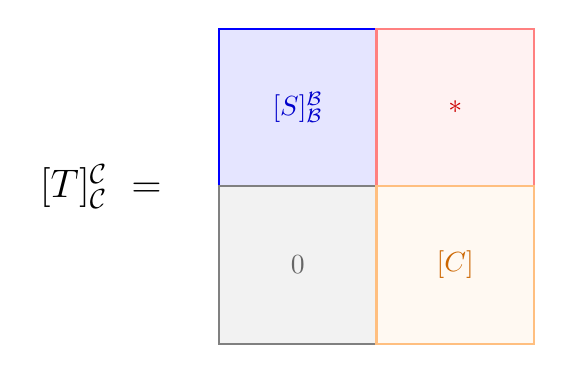
\begin{tikzpicture}
      % Main matrix frame
      \draw[thick] (0,0) rectangle (4,4);

      % Block 1: The Cyclic Subspace
      \filldraw[fill=blue!10, draw=blue, thick] (0,2) rectangle (2,4);
      \node[blue!80!black] at (1,3) {$[S]_{\mathcal{B}}^{\mathcal{B}}$};

      % Block 2: The arbitrary upper right
      \filldraw[fill=red!5, draw=red!50, thick] (2,2) rectangle (4,4);
      \node[red!80!black] at (3,3) {$\ast$};

      % Block 3: The forced zero block (due to invariance)
      \filldraw[fill=gray!10, draw=gray, thick] (0,0) rectangle (2,2);
      \node[gray!80!black] at (1,1) {$0$};

      % Block 4: The arbitrary lower right
      \filldraw[fill=orange!5, draw=orange!50, thick] (2,0) rectangle (4,2);
      \node[orange!80!black] at (3,1) {$[C]$};

      % Label
      \node at (-1.5, 2) {\Large $[T]_{\mathcal{C}}^{\mathcal{C}} \ = $};
    \end{tikzpicture}
  \end{center}
  Because the determinant of a block-triangular matrix is the product of the determinants of its diagonal blocks, we have $P_T(x) = P_S(x) \cdot P_C(x)$. Consider the endomorphism $R := P_T(T) \in \End(V)$. Since polynomials evaluated at $T$ commute with one another, we can factor $R$:
  \[
  R = P_C(T) \circ P_S(T).
  \]
  Therefore, $Rv = P_C(T) \Big( P_S(T)v \Big)$.
  However, applying Lemma \ref{lemma:companion_char_poly} directly to $v$:
  \[
  P_S(T)v = (-1)^d (T^d v - c_{d-1}T^{d-1}v - \dots - c_0 v).
  \]
  By the very definition of our constants $c_i$, this evaluates exactly to $0$. Hence $Rv = P_C(T)(0) = 0$. Since $v \neq 0$ was chosen completely arbitrarily, $P_T(T)$ evaluates to zero on every vector in $V$, meaning $P_T(T) = 0$.
\end{proof}

\begin{remark}[The Lazy Proof]\label{rem:lazy_proof}
  A completely incorrect "proof" often presented by students is: $P_A(A) = \det(A - A \cdot I) = \det(0) = 0$. This is fundamentally invalid. The expression $P_A(x) = \det(A - xI)$ evaluates to a polynomial with scalar coefficients. Substituting matrices into a scalar expression \textit{before} expanding the determinant leads to a severe category error. One must compute the scalar polynomial first, and only then evaluate it at the matrix $A$.
\end{remark}
\setcounter{chapter}{21}
\renewcommand{\thetheorem}{22.a.\arabic{theorem}}
\setcounter{theorem}{0}

\chapter{Euclidean and Hermitian Spaces}

\section{Euclidean and Hermitian (Unitary) Spaces}

At last (!) we endow our spaces with a geometric structure. We work here with vector spaces $V$ over $K = \mathbb{R}$ or $K = \mathbb{C}$. Over $\mathbb{R}$, we will have \qt{Euclidean spaces}. Over $\mathbb{C}$, we will have \qt{Hermitian} (a.k.a.\ unitary) spaces.

% def 22.a.1
\begin{definition}[Scalar Product over $\mathbb{R}$]
\label{def:scalar_product_real}
Let $V$ be a vector space over $\mathbb{R}$. A \qt{scalar product} (a.k.a.\ \qt{inner product}) is a function $V \times V \longrightarrow \mathbb{R}$, denoted by $v, w \mapsto \langle v, w \rangle$ (or $(v,w)$), that has the following properties:
\begin{enumerate}
    \item \textbf{Linearity in the first variable:}
    \begin{align*}
        \langle v_1 + v_2, w \rangle &= \langle v_1, w \rangle + \langle v_2, w \rangle \quad \forall v_1, v_2, w \in V \\
        \langle \alpha v, w \rangle &= \alpha \langle v, w \rangle \quad \forall \alpha \in \mathbb{R}, \; \forall v, w \in V
    \end{align*}
    \item \textbf{Linearity in the second variable:}
    \begin{align*}
        \langle v, w_1 + w_2 \rangle &= \langle v, w_1 \rangle + \langle v, w_2 \rangle \quad \forall v, w_1, w_2 \in V \\
        \langle v, \alpha w \rangle &= \alpha \langle v, w \rangle \quad \forall \alpha \in \mathbb{R}, \; \forall v, w \in V
    \end{align*}
    \item \textbf{Symmetry:}
    \[
        \langle v, w \rangle = \langle w, v \rangle \quad \forall v, w \in V
    \]
    \item \textbf{Positivity:}
    \[
        0 \neq v \in V \implies \langle v, v \rangle > 0
    \]
\end{enumerate}
We call $(V, \langle \cdot, \cdot \rangle)$ a \qt{Euclidean space}, or a space endowed with a scalar product.
\end{definition}

% def 22.a.2
\begin{definition}[Hermitian Product over $\mathbb{C}$]
\label{def:hermitian_product_complex}
Let $V$ be a vector space over $\mathbb{C}$. A \qt{Hermitian product} (or \qt{inner product}) on $V$ is a function $V \times V \longrightarrow \mathbb{C}$, denoted by $v, w \mapsto \langle v, w \rangle$, with the following properties:
\begin{enumerate}
    \item \textbf{Linearity in the first variable:}
    \begin{align*}
        \langle v_1 + v_2, w \rangle &= \langle v_1, w \rangle + \langle v_2, w \rangle \quad \forall v_1, v_2, w \in V \\
        \langle \alpha v, w \rangle &= \alpha \langle v, w \rangle \quad \forall \alpha \in \mathbb{C}, \; \forall v, w \in V
    \end{align*}
    \item \textbf{Sesquilinearity/Conjugate-linearity (complex anti-linearity) in the second variable:}
    \begin{align*}
        \langle v, w_1 + w_2 \rangle &= \langle v, w_1 \rangle + \langle v, w_2 \rangle \quad \forall v, w_1, w_2 \in V \\
        \langle v, \alpha w \rangle &= \overline{\alpha} \langle v, w \rangle \quad \forall \alpha \in \mathbb{C}, \; \forall v, w \in V
    \end{align*}
    \item \textbf{Hermitian property:}
    \[
        \langle v, w \rangle = \overline{\langle w, v \rangle} \quad \forall v, w \in V
    \]
    \item \textbf{Positivity:}
    \[
        0 \neq v \in V \implies \langle v, v \rangle > 0
    \]
\end{enumerate}
We call $(V, \langle \cdot, \cdot \rangle)$ a \qt{Hermitian} (or unitary) space.
\end{definition}

% remark
\begin{remark}[Complex Conjugate and Inner Products]
Recall that if $\alpha = a + ib \in \mathbb{C}$, where $a, b \in \mathbb{R}$ and $i = \sqrt{-1}$, then $\overline{\alpha} := a - ib$ is the complex conjugate of $\alpha$. Recall also, that $\alpha \cdot \overline{\alpha} = a^2 + b^2 = |\alpha|^2 \geq 0$, with equality if and only if $\alpha = 0$.

Note that the definition of a Hermitian product coincides with a scalar product if $V$ is over $\mathbb{R}$, and we allow $\alpha$ only in $\mathbb{R}$.
\end{remark}

% lemma 22.a.3
\begin{lemma}[Basic Properties of the Inner Product]
Let $V$ be a Euclidean or Hermitian vector space. Then:
\begin{enumerate}
    \item $\forall v \in V$, $\langle 0, v \rangle = \langle v, 0 \rangle = 0$.
    \item Let $w \in V$. If $\langle v, w \rangle = 0$ for all $v \in V$, then $w = 0$. (Exercise)
    \item Let $w_1, w_2 \in V$. If $\langle v, w_1 \rangle = \langle v, w_2 \rangle$ for all $v \in V$, then $w_1 = w_2$.
\end{enumerate}
\end{lemma}

% def 22.a.4
\begin{definition}[Norm, Distance, and Orthogonality]
\label{def:norm_distance_orthogonality}
Let $V$ be a Euclidean or Hermitian vector space.
\begin{enumerate}
    \item For all $v \in V$, we define $\|v\| := \sqrt{\langle v, v \rangle} \in \mathbb{R}_{\geq 0}$. The function $\| \cdot \|$ is called the \qt{norm} on $V$ induced by $\langle \cdot, \cdot \rangle$.
    \item A vector $u \in V$ is called a \qt{unit vector} if $\|u\| = 1$. Note that if $0 \neq v \in V$ is any vector, then $\frac{1}{\|v\|}v$ is a unit vector (which is positively proportional to $v$, so it points in the same direction as $v$). We call $\frac{v}{\|v\|}$ the \qt{normalization} of $v$.
    \item For $v, w \in V$, we define the \qt{distance} between $v$ and $w$ by $d(v, w) := \|v - w\|$.
    \item Two vectors $v, w \in V$ are called \qt{orthogonal} (or perpendicular to one another) if $\langle v, w \rangle = 0$. If this is the case, we sometimes write $v \perp w$.
    \item A subset $S \subseteq V$ is called an \qt{orthogonal system} if $0 \notin S$, and for every two distinct elements $v, w \in S$, we have $v \perp w$.
    \item An orthogonal system $S \subseteq V$ is called \qt{orthonormal} if for all $u \in S$, we have $\|u\| = 1$.
\end{enumerate}
\end{definition}

% thm 22.a.5
\begin{theorem}[Pythagoras' Theorem]
\label{thm:pythagoras}
Let $V$ be a Euclidean or Hermitian vector space, and let $v, w \in V$ with $v \perp w$. Then:
\[
    \|v + w\|^2 = \|v\|^2 + \|w\|^2
\]
\end{theorem}

\begin{center}
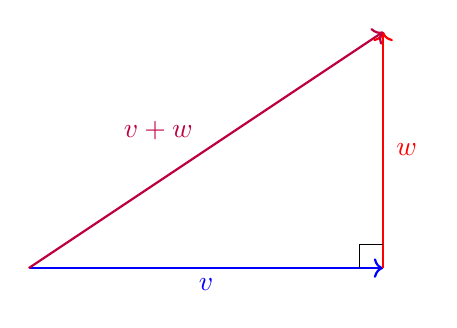
\begin{tikzpicture}[scale=1.5]
    % Define points
    \coordinate (O) at (0,0);
    \coordinate (V) at (3,0);
    \coordinate (VW) at (3,2);
    
    % Draw vectors
    \draw[->, thick, blue] (O) -- (V) node[midway, below] {$v$};
    \draw[->, thick, red] (V) -- (VW) node[midway, right] {$w$};
    \draw[->, thick, purple] (O) -- (VW) node[midway, above left] {$v+w$};
    
    % Right angle symbol
    \draw (2.8, 0) -- (2.8, 0.2) -- (3, 0.2);
\end{tikzpicture}
\end{center}

\begin{proof}
By definition of the norm and the properties of the inner product, we have:
\begin{align*}
    \|v + w\|^2 &= \langle v + w, v + w \rangle \\
    &= \langle v, v \rangle + \langle v, w \rangle + \langle w, v \rangle + \langle w, w \rangle
\end{align*}
Since $v \perp w$, we know that $\langle v, w \rangle = 0$. By Hermitian symmetry, this also implies $\langle w, v \rangle = \overline{\langle v, w \rangle} = \overline{0} = 0$. Therefore, the cross terms vanish, leaving us with:
\begin{align*}
    \|v + w\|^2 &= \|v\|^2 + 0 + 0 + \|w\|^2 \\
    &= \|v\|^2 + \|w\|^2
\end{align*}
\end{proof}

% exercise 1
\begin{exercise}[Generalized Pythagoras' Theorem]
Let $v_1, \dots, v_k \in V$ (where $V$ is a Euclidean or Hermitian space) be mutually orthogonal (i.e., $\langle v_i, v_j \rangle = 0$ for $i \neq j$). Then:
\[
    \|v_1 + \dots + v_k\|^2 = \sum_{i=1}^k \|v_i\|^2
\]
\end{exercise}

% exercise 2
\begin{exercise}[Linear Independence of Orthogonal Systems]
Let $V$ be a Euclidean or Hermitian space. Show that any orthogonal system $S \subseteq V$ is linearly independent.
\end{exercise}

% exercise (page 4)
\begin{exercise}[Reconstructing the Scalar Product from the Norm]
Let $V$ be a Euclidean space. Show that for all $u, v \in V$, we have:
\[
    \langle u, v \rangle = \frac{1}{2}\left(\|u+v\|^2 - \|u\|^2 - \|v\|^2\right) \quad (*)
\]
This shows that the norm $\|\cdot\|$ completely determines the scalar product $\langle\cdot,\cdot\rangle$.
\end{exercise}

% exercise (page 4)
\begin{exercise}[Polarization Identity]
Let $V$ be a Hermitian space. Then:
\[
    \langle u, v \rangle = \frac{1}{4}\left(\|u+v\|^2 - \|u-v\|^2 + i\|u+iv\|^2 - i\|u-iv\|^2\right) \quad (**)
\]
\end{exercise}

\begin{importantremark}[The Parallelogram Law]
\label{rem:parallelogram_law}
Warning: For general norms $\|\cdot\|$, one cannot necessarily find a scalar product that induces it. A norm $\|\cdot\|$ comes from a scalar product if and only if it satisfies the \qt{Parallelogram law}:
\[
    \|u+v\|^2 + \|u-v\|^2 = 2\left(\|u\|^2 + \|v\|^2\right)
\]
\end{importantremark}

\subsection{Examples}

% examples (page 5)
\begin{example}[Standard and Matrix-Induced Inner Products]
\leavevmode
\begin{enumerate}
    \item Standard inner products on $\mathbb{R}^n$ and $\mathbb{C}^n$:
    \begin{align*}
        \langle x, y \rangle_{\mathbb{R}^n} &= \sum_{i=1}^n x_i y_i \\
        \langle z, w \rangle_{\mathbb{C}^n} &= \sum_{i=1}^n z_i \overline{w}_i
    \end{align*}
    
    \item Let $A \in \M_{n \times n}(\mathbb{R})$ be a symmetric matrix. Define a function $V \times V \longrightarrow \mathbb{R}$ by:
    \[
        \langle v, w \rangle_A = v^T A w
    \]
    Check that properties (1)--(3) of a scalar product hold for \textit{any} symmetric matrix $A$. Specifically, for symmetry, we have:
    \[
        \langle w, v \rangle_A = w^T A v = (w^T A v)^T = v^T A^T w = v^T A w = \langle v, w \rangle_A
    \]
    (Note that $w^T A v$ is a $1 \times 1$ matrix, and is therefore equal to its transpose).
    
    What about property (4), positivity? For example, let $A = \begin{pmatrix} 1 & 0 \\ 0 & -1 \end{pmatrix}$, which is symmetric. Then:
    \[
        \left\langle \begin{pmatrix} x_1 \\ x_2 \end{pmatrix}, \begin{pmatrix} y_1 \\ y_2 \end{pmatrix} \right\rangle_A = x_1 y_1 - x_2 y_2
    \]
    But taking $v = \begin{pmatrix} 0 \\ 1 \end{pmatrix}$, we get:
    \[
        \left\langle \begin{pmatrix} 0 \\ 1 \end{pmatrix}, \begin{pmatrix} 0 \\ 1 \end{pmatrix} \right\rangle_A = -1 < 0
    \]
    So, there is a lack of positivity.
\end{enumerate}
\end{example}




\subsection{Matrices and Positive Definiteness}

% Def. (22.a.6)
\begin{definition}[Symmetric Matrix]
    A matrix $A \in \M_{n \times n}(K)$ (where $K$ is any field) is called \qt{symmetric} if $A^T = A$ (i.e., $a_{ij} = a_{ji}$ for all $i,j$).
\end{definition}

% Def. (22.a.7)
\begin{definition}[Adjoint and Hermitian Matrices]
    \begin{enumerate}
        \item Let $A \in \M_{n \times m}(\mathbb{C})$. We write $\overline{A}$ for the matrix whose entry at index $(i,j)$ is $\overline{A_{ij}}$, representing complex conjugation. Thus, $(\overline{A})_{ij} := \overline{A_{ij}}$.
        \item Let $A \in \M_{n \times m}(\mathbb{C})$. We define $A^* := \overline{A}^T \in \M_{m \times n}(\mathbb{C})$. The matrix $A^*$ is called the \qt{adjoint matrix} of $A$ (this has nothing to do with the classical adjoint, $\operatorname{adj}(A)$).
        \item A matrix $A \in \M_{n \times n}(\mathbb{C})$ is called \qt{Hermitian} if $A^* = A$ (which is equivalent to $A = \overline{A}^T$).
    \end{enumerate}
\end{definition}

\begin{example}[Important example]
    Let $A \in \M_{n \times n}(\mathbb{R})$. Define $\langle \cdot, \cdot \rangle_A : \mathbb{R}^n \times \mathbb{R}^n \to \mathbb{R}$ by
    \begin{equation*}
        \langle v, w \rangle_A = v^T \cdot A \cdot w.
    \end{equation*}
    
    \begin{exercise}
        Show that $\langle \cdot, \cdot \rangle_A$ is bilinear (i.e., linear in both variables).
    \end{exercise}
    
    Assume now that $A$ is symmetric. Then, $\langle v, w \rangle_A = \langle w, v \rangle_A$ for all $v, w$. Indeed,
    \begin{equation*}
        \langle w, v \rangle_A = w^T \cdot A \cdot v = w^T A^T v = (v^T A w)^T = (\langle v, w \rangle_A)^T = \langle v, w \rangle_A.
    \end{equation*}
    (Note that $v^T A w$ is just a scalar, which can be viewed as a $1 \times 1$ matrix, hence it equals its own transpose). 
    
    Is $\langle \cdot, \cdot \rangle_A$ a scalar product? In general, it is not. For example, consider $A = \left(\begin{smallmatrix} -1 & 0 \\ 0 & -1 \end{smallmatrix}\right)$. Then, $\langle \left(\begin{smallmatrix} 0 \\ 1 \end{smallmatrix}\right), \left(\begin{smallmatrix} 0 \\ 1 \end{smallmatrix}\right) \rangle_A = -1$. However, for a scalar product, we need $\langle v, v \rangle > 0$ for all $v \neq 0$. Therefore, we lack positivity here.
\end{example}

% Def. (22.a.8)
\begin{definition}[Positive Definite Matrix (Real Case)]
    A symmetric matrix $A \in \M_{n \times n}(\mathbb{R})$ is called \qt{positive definite} if $v^T A v > 0$ for all $0 \neq v \in \mathbb{R}^n$.
\end{definition}

\begin{claim*}
    If $A$ is positive definite, then $\langle \cdot, \cdot \rangle_A$ is a scalar product.
\end{claim*}

\begin{example}
    \begin{enumerate}
        \item Let $a_1, \dots, a_n > 0$ (with $a_i \in \mathbb{R}$). Then, the diagonal matrix
        \begin{equation*}
            D = \begin{pmatrix} a_1 & & 0 \\ & \ddots & \\ 0 & & a_n \end{pmatrix}
        \end{equation*}
        is positive definite. Indeed, if $v = \begin{pmatrix} v_1 \\ \vdots \\ v_n \end{pmatrix}$, then
        \begin{equation*}
            \langle v, v \rangle_D = v^T \cdot D \cdot v = a_1 v_1^2 + \dots + a_n v_n^2 \geq 0,
        \end{equation*}
        with equality if and only if $v_i = 0$ for all $i$.
        \item Let $A = \begin{pmatrix} a & b \\ b & d \end{pmatrix} \in \M_{2 \times 2}(\mathbb{R})$. Then, $A$ is positive definite if and only if $a > 0$ and $\det(A) > 0$ (Exercise).
    \end{enumerate}
\end{example}

The situation for Hermitian products is similar.

% Def. (22.a.9)
\begin{definition}[Positive Definite Matrix (Complex Case)]
    Let $A \in \M_{n \times n}(\mathbb{C})$ be a Hermitian matrix. We say that $A$ is \qt{positive definite} if for all $0 \neq v \in \mathbb{C}^n$, we have $v^T A \overline{v} > 0$. 
\end{definition}

\begin{remark}
    Note that $v^T A \overline{v} \in \mathbb{R}$, because
    \begin{equation*}
        \overline{(v^T A \overline{v})} = \overline{v}^T \overline{A} v = (\overline{v}^T \overline{A} v)^T = v^T \overline{A}^T \overline{v} = v^T A \overline{v}.
    \end{equation*}
    Here, we used the facts that for a $1 \times 1$ matrix (a scalar), $(\cdot)^T = (\cdot)$, and that $A$ is Hermitian (so $\overline{A}^T = A$). Also, recall that if $v = \begin{pmatrix} v_1 \\ \vdots \\ v_n \end{pmatrix} \in \mathbb{C}^n$, then $\overline{v} := \begin{pmatrix} \overline{v}_1 \\ \vdots \\ \overline{v}_n \end{pmatrix}$.
\end{remark}

Given a positive definite complex matrix $A$, we can define a Hermitian product on $\mathbb{C}^n$ by
\begin{equation*}
    \langle v, w \rangle_A = v^T A \overline{w}.
\end{equation*}

\begin{claim*}
    The operation $\langle \cdot, \cdot \rangle_A$ is a Hermitian product if and only if $A$ is positive definite.
\end{claim*}

\begin{exercise}
    A matrix $A = \begin{pmatrix} a & b \\ \overline{b} & d \end{pmatrix} \in \M_{2 \times 2}(\mathbb{C})$ is positive definite if and only if $a > 0$, $\det A \in \mathbb{R}$, and $\det A > 0$.
\end{exercise}

\begin{proof}[Proof of the Claim]
    We will prove it for complex matrices and Hermitian products (the case of symmetric matrices and scalar products is very similar and even simpler, which is left as an exercise). 
    
    Let $A \in \M_{n \times n}(\mathbb{C})$ and suppose that $\langle v, w \rangle_A := v^T A \overline{w}$ is a Hermitian product. For all $v, w$, we have 
    \begin{equation}\langle v, w \rangle_A = \overline{\langle w, v \rangle}_A,\end{equation} 
    which implies
    \begin{equation*}
        v^T A \overline{w} = \overline{w^T A \overline{v}}.
    \end{equation*}
    This simplifies as follows:
    \begin{equation*}
        v^T A \overline{w} = \overline{w}^T \overline{A} v \implies v^T A \overline{w} = (\overline{w}^T \overline{A} v)^T \implies v^T A \overline{w} = v^T \overline{A}^T \overline{w}.
    \end{equation*}
    Take $v = e_i$ and $w = e_j$ (the standard basis vectors). Write $A$ as
    \begin{equation*}
        A = \begin{pmatrix} a_{11} & \dots & a_{1j} & \dots & a_{1n} \\ \vdots & & \vdots & & \vdots \\ a_{n1} & \dots & a_{nj} & \dots & a_{nn} \end{pmatrix}.
    \end{equation*}
    Then,
    \begin{equation*}
        e_i^T \cdot A \cdot e_j = \begin{pmatrix} 0 & \dots & 1 & \dots & 0 \end{pmatrix} A \begin{pmatrix} 0 \\ \vdots \\ 1 \\ \vdots \\ 0 \end{pmatrix} = \begin{pmatrix} 0 & \dots & 1 & \dots & 0 \end{pmatrix} \begin{pmatrix} a_{1j} \\ \vdots \\ a_{nj} \end{pmatrix} = a_{ij}.
    \end{equation*}
    Similarly, $e_i^T \overline{A}^T e_j = \overline{a}_{ji}$. Therefore, $a_{ij} = \overline{a}_{ji}$ for all $i, j$, which means $\overline{A}^T = A$, proving that $A$ is Hermitian. 
    
    The fact that $A$ is positive definite is precisely the condition that $\langle v, v \rangle_A > 0$ for all $v \neq 0$, which translates to $v^T A \overline{v} > 0$.
    
    The opposite statement, that if $A$ is positive definite then $\langle \cdot, \cdot \rangle_A$ is a Hermitian product, is left as an exercise.
\end{proof}

\subsection{The geometry on $V$ and the choice of inner product}

The geometry on $V$ depends on the choice of inner product.

\begin{example}
    Let $V = \mathbb{R}^2$. Let $\langle v, w \rangle = v_1 w_1 + v_2 w_2$ be the standard scalar product on $\mathbb{R}^2$. 
    We define another product $\langle v, w \rangle' = a_1 v_1 w_1 + a_2 v_2 w_2$, where $a_1, a_2 > 0$. 
    Notice that this is exactly $\langle v, w \rangle_A$ for the matrix $A = \begin{pmatrix} a_1 & 0 \\ 0 & a_2 \end{pmatrix}$.
    
    The unit sphere for the standard product $\langle \cdot, \cdot \rangle$ is:
    \begin{equation*}
        S = \{v \in \mathbb{R}^2 \mid \|v\| = 1\} = \{(v_1, v_2) \mid v_1^2 + v_2^2 = 1\}.
    \end{equation*}
    The unit sphere for $\langle \cdot, \cdot \rangle'$ is:
    \begin{equation*}
        S' = \{v \in \mathbb{R}^2 \mid \|v\|' = 1\} = \{(v_1, v_2) \mid a_1 v_1^2 + a_2 v_2^2 = 1\}.
    \end{equation*}

    \begin{center}
        \begin{minipage}{0.45\textwidth}
            \centering
            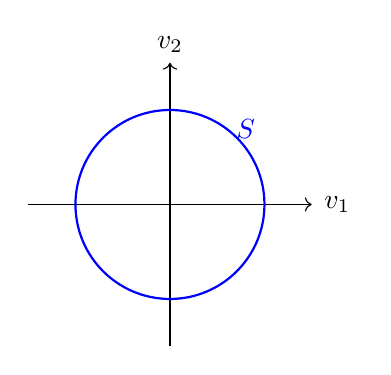
\begin{tikzpicture}[scale=1.2]
                \draw[->] (-1.5,0) -- (1.5,0) node[right] {$v_1$};
                \draw[->] (0,-1.5) -- (0,1.5) node[above] {$v_2$};
                \draw[thick, blue] (0,0) circle (1);
                \node[blue] at (0.8, 0.8) {$S$};
            \end{tikzpicture}
        \end{minipage}
        \begin{minipage}{0.45\textwidth}
            \centering
            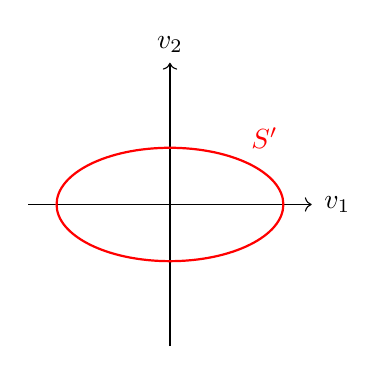
\begin{tikzpicture}[scale=1.2]
                \draw[->] (-1.5,0) -- (1.5,0) node[right] {$v_1$};
                \draw[->] (0,-1.5) -- (0,1.5) node[above] {$v_2$};
                \draw[thick, red] (0,0) ellipse (1.2 and 0.6);
                \node[red] at (1.0, 0.7) {$S'$};
            \end{tikzpicture}
        \end{minipage}
    \end{center}
\end{example}

\begin{example}
    Let $A = \begin{pmatrix} 1 & -1 \\ -1 & 2 \end{pmatrix}$. This matrix is positive definite (why?). 
    Let $\langle \cdot, \cdot \rangle$ be the standard scalar product, and define $\langle \cdot, \cdot \rangle' := \langle \cdot, \cdot \rangle_A$.
    
    We compute:
    \begin{equation*}
        \left\langle \begin{pmatrix} 1 \\ 0 \end{pmatrix}, \begin{pmatrix} 1 \\ 1 \end{pmatrix} \right\rangle = 1.
    \end{equation*}
    However, using the modified product:
    \begin{equation*}
        \left\langle \begin{pmatrix} 1 \\ 0 \end{pmatrix}, \begin{pmatrix} 1 \\ 1 \end{pmatrix} \right\rangle' = \begin{pmatrix} 1 & 0 \end{pmatrix} \begin{pmatrix} 1 & -1 \\ -1 & 2 \end{pmatrix} \begin{pmatrix} 1 \\ 1 \end{pmatrix} = \begin{pmatrix} 1 & -1 \end{pmatrix} \begin{pmatrix} 1 \\ 1 \end{pmatrix} = 0.
    \end{equation*}
    So, $\left(\begin{smallmatrix} 1 \\ 0 \end{smallmatrix}\right) \perp' \left(\begin{smallmatrix} 1 \\ 1 \end{smallmatrix}\right)$, but $\left(\begin{smallmatrix} 1 \\ 0 \end{smallmatrix}\right) \not\perp \left(\begin{smallmatrix} 1 \\ 1 \end{smallmatrix}\right)$.

    \begin{center}
        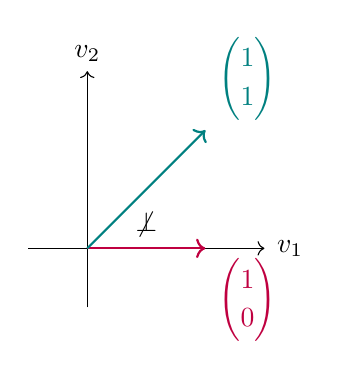
\begin{tikzpicture}[scale=1.5]
            \draw[->] (-0.5,0) -- (1.5,0) node[right] {$v_1$};
            \draw[->] (0,-0.5) -- (0,1.5) node[above] {$v_2$};
            \draw[->, thick, purple] (0,0) -- (1,0) node[below right] {$\begin{pmatrix} 1 \\ 0 \end{pmatrix}$};
            \draw[->, thick, teal] (0,0) -- (1,1) node[above right] {$\begin{pmatrix} 1 \\ 1 \end{pmatrix}$};
            \node at (0.5, 0.2) {$\not\perp$};
        \end{tikzpicture}
    \end{center}
\end{example}

\subsection{A different type of example}

\begin{example}[A different type of example]
    Let $C[a,b]$ be the space of continuous functions $f: [a,b] \to \mathbb{R}$. It is a vector space over $\mathbb{R}$ with respect to the standard operations. 
    We define a scalar product:
    \begin{equation*}
        \langle f, g \rangle := \int_a^b f(x) \cdot g(x) \, dx.
    \end{equation*}
    This is well-defined and finite. (Why?)
\end{example}

\begin{exercise}
    Show that $\langle \cdot, \cdot \rangle$ is linear in both variables and symmetric.
\end{exercise}

Let us check positivity: let $0 \neq f \in C[a,b]$.
\begin{equation*}
    \langle f, f \rangle = \int_a^b (f(x))^2 \, dx.
\end{equation*}
Since $f \neq 0$, there exists an $x_0 \in (a,b)$ such that $f(x_0) \neq 0$. Since $f$ is continuous, so is $f^2$. Hence, there exists a $\delta > 0$ such that $[x_0 - \delta, x_0 + \delta] \subseteq [a,b]$ and $f(x) \neq 0$ for all $x \in [x_0 - \delta, x_0 + \delta]$. This implies that $(f(x))^2 > 0$ for all $x \in [x_0 - \delta, x_0 + \delta]$. Therefore,

\begin{equation*}
    \langle f, f \rangle = \int_a^b (f(x))^2 \, dx \geq \int_{x_0 - \delta}^{x_0 + \delta} (f(x))^2 \, dx \geq 2\delta \cdot \min_{x \in [x_0-\delta, x_0+\delta]} (f(x))^2 > 0.
\end{equation*}

\begin{remark}
    By this scalar product on $C[-\pi, \pi]$, the functions $f(x) = \sin x$ and $g(x) \equiv 1$ are orthogonal.
\end{remark}

\subsection{Norms and Angles}

% Def. (22.a.10)
\begin{definition}[Norm]
    Let $V$ be a vector space over $K$ (where $K = \mathbb{R}$ or $\mathbb{C}$). A \qt{norm} on $V$ is a function $\| \cdot \|: V \to \mathbb{R}_{\geq 0}$ such that:
    \begin{enumerate}
        \item $\|u + v\| \leq \|u\| + \|v\|$ for all $u, v \in V$ (Triangle inequality).
        \item $\|\alpha \cdot v\| = |\alpha| \cdot \|v\|$ for all $\alpha \in K$ and $v \in V$ (Homogeneity).
        \item If $\|v\| = 0$, then $v = 0$ (Non-degeneracy).
    \end{enumerate}
\end{definition}

\begin{claim*}
    If $\langle \cdot, \cdot \rangle$ is an inner product on $V$, then $\|v\| := \sqrt{\langle v, v \rangle}$ is a norm on $V$. We will prove this soon.
\end{claim*}

\begin{exercise}
    For $\left(\begin{smallmatrix} a \\ b \end{smallmatrix}\right) \in \mathbb{R}^2$, define $\left\| \left(\begin{smallmatrix} a \\ b \end{smallmatrix}\right) \right\|' := \max\{|a|, |b|\}$, and $\left\| \left(\begin{smallmatrix} a \\ b \end{smallmatrix}\right) \right\|'' := |a| + |b|$. 
    Show that $\| \cdot \|'$ and $\| \cdot \|''$ are norms, but they are not induced by any scalar product. 
    
    \textit{Hint:} Recall that if the scalar product $\langle \cdot, \cdot \rangle$ induces $\| \cdot \|$, then $\langle u, w \rangle = \frac{1}{2} (\|u + w\|^2 - \|u\|^2 - \|w\|^2)$.
\end{exercise}

% Thm. (22.a.11)
\begin{theorem}[Cauchy-Schwarz Inequality]
    \label{thm:cauchy_schwarz}
    Let $V$ be a Euclidean or Hermitian space. For all $u, v \in V$, we have
    \begin{equation*}
        |\langle u, v \rangle| \leq \|u\| \cdot \|v\|.
    \end{equation*}
    Furthermore, equality holds if and only if $u$ and $v$ are linearly dependent.
\end{theorem}

\begin{proof}
    If $v = 0$, then both sides are $0$, and the inequality holds (with equality). Since $v = 0$, the vectors $u$ and $v$ are linearly dependent, and therefore, the second statement also holds.
    
    Assume now that $v \neq 0$. For any scalar $\lambda \in K$ (where $K = \mathbb{R}$ or $\mathbb{C}$), we have, by the positivity of the inner product,
    \begin{equation*}
        0 \leq \langle u - \lambda v, u - \lambda v \rangle.
    \end{equation*}
    Using the linearity in the first variable and conjugate-linearity (or linearity) in the second variable, we expand this to obtain
    \begin{equation*}
        0 \leq \langle u, u \rangle - \lambda \langle v, u \rangle - \overline{\lambda} \langle u, v \rangle + \lambda \overline{\lambda} \langle v, v \rangle.
    \end{equation*}
    Choose $\lambda = \frac{\langle u, v \rangle}{\|v\|^2}$. Substituting this into the inequality yields
    \begin{align*}
        0 &\leq \|u\|^2 - \frac{\langle u, v \rangle}{\|v\|^2} \langle v, u \rangle - \frac{\overline{\langle u, v \rangle}}{\|v\|^2} \langle u, v \rangle + \frac{\langle u, v \rangle \overline{\langle u, v \rangle}}{\|v\|^4} \|v\|^2 \\
        &= \|u\|^2 - \frac{\langle u, v \rangle \overline{\langle u, v \rangle}}{\|v\|^2} - \frac{\overline{\langle u, v \rangle} \langle u, v \rangle}{\|v\|^2} + \frac{\langle u, v \rangle \overline{\langle u, v \rangle}}{\|v\|^2} \\
        &= \|u\|^2 - \frac{|\langle u, v \rangle|^2}{\|v\|^2}.
    \end{align*}
    Multiplying by $\|v\|^2$ (which is strictly positive), we obtain
    \begin{equation*}
        0 \leq \|u\|^2 \|v\|^2 - |\langle u, v \rangle|^2 \implies |\langle u, v \rangle|^2 \leq \|u\|^2 \|v\|^2.
    \end{equation*}
    Taking the square root of both sides gives the Cauchy-Schwarz inequality.
    
    For the equality condition, notice that equality holds if and only if $\langle u - \lambda v, u - \lambda v \rangle = 0$. By the non-degeneracy of the inner product, this is equivalent to $u - \lambda v = 0$, meaning $u = \lambda v$. Therefore, equality holds if and only if $u$ and $v$ are linearly dependent.
\end{proof}

% Cor. (22.a.12)
\begin{corollary}
    If $\langle \cdot, \cdot \rangle$ is an inner product on $V$, then $\|v\| := \sqrt{\langle v, v \rangle}$ is a norm on $V$.
\end{corollary}

\begin{proof}
    The positivity and homogeneity properties are straightforward to verify. We will show the triangle inequality, namely $\|u + v\| \leq \|u\| + \|v\|$. We compute
    \begin{align*}
        \|u + v\|^2 &= \langle u + v, u + v \rangle \\
        &= \langle u, u \rangle + \langle u, v \rangle + \langle v, u \rangle + \langle v, v \rangle \\
        &= \|u\|^2 + \langle u, v \rangle + \overline{\langle u, v \rangle} + \|v\|^2 \\
        &= \|u\|^2 + 2 \operatorname{Re}(\langle u, v \rangle) + \|v\|^2.
    \end{align*}
    Since $\operatorname{Re}(z) \leq |z|$ for any complex number $z$, and applying the Cauchy-Schwarz inequality, we get
    \begin{equation*}
        \|u + v\|^2 \leq \|u\|^2 + 2 |\langle u, v \rangle| + \|v\|^2 \leq \|u\|^2 + 2 \|u\| \|v\| + \|v\|^2 = (\|u\| + \|v\|)^2.
    \end{equation*}
    Taking the square root yields the desired result.
\end{proof}

% Def. (22.a.13)
\begin{definition}[Angle]
    Let $V$ be a Euclidean space. For any two non-zero vectors $u, v \in V$, we define the \qt{angle} $\alpha$ between them by the equation
    \begin{equation*}
        \cos \alpha = \frac{\langle u, v \rangle}{\|u\| \cdot \|v\|},
    \end{equation*}
    where $\alpha \in [0, \pi]$. The Cauchy-Schwarz inequality guarantees that $-1 \leq \frac{\langle u, v \rangle}{\|u\| \cdot \|v\|} \leq 1$, so this definition is well-posed.
\end{definition}

\begin{definition*}[Orthogonality]
    Let $V$ be a Euclidean or Hermitian space. We say that $u, v \in V$ are \qt{orthogonal} if $\langle u, v \rangle = 0$. In this case, we write $u \perp v$.
\end{definition*}

\begin{example}
    In $\mathbb{R}^2$ with the standard scalar product, the vectors $e_1 = \left(\begin{smallmatrix} 1 \\ 0 \end{smallmatrix}\right)$ and $e_2 = \left(\begin{smallmatrix} 0 \\ 1 \end{smallmatrix}\right)$ are orthogonal.
\end{example}

\begin{remark}
    The relationship between orthogonality and the norm is captured by the Pythagorean Theorem (Theorem \ref{thm:pythagoras}), which states that for orthogonal vectors $u$ and $v$, the squared norm of their sum is the sum of their squared norms: $\|u+v\|^2 = \|u\|^2 + \|v\|^2$.
\end{remark}


\subsection{The Gram-Schmidt Orthogonalization Process}

% Thm. (22.a.14)
\begin{theorem}[Properties of Orthogonal Systems]
    Let $V$ be a Euclidean or Hermitian space, and let $(v_1, \dots, v_k)$ be an orthogonal system of non-zero vectors in $V$. Then:
    \begin{itemize}
        \item The vectors $v_1, \dots, v_k$ are linearly independent.
        \item If $v \in \Sp(v_1, \dots, v_k)$, meaning $v = \sum_{i=1}^k \alpha_i v_i$, then the coefficients are given by
        \begin{equation*}
            \alpha_i = \frac{\langle v, v_i \rangle}{\|v_i\|^2} \quad \text{for all } 1 \leq i \leq k.
        \end{equation*}
    \end{itemize}
\end{theorem}

\begin{proof}
    We prove the second property first. Suppose $v = \sum_{j=1}^k \alpha_j v_j$. Taking the inner product with $v_i$ yields
    \begin{equation*}
        \langle v, v_i \rangle = \left\langle \sum_{j=1}^k \alpha_j v_j, v_i \right\rangle = \sum_{j=1}^k \alpha_j \langle v_j, v_i \rangle.
    \end{equation*}
    Since the system is orthogonal, $\langle v_j, v_i \rangle = 0$ for all $j \neq i$. Thus, the sum collapses to a single term:
    \begin{equation*}
        \langle v, v_i \rangle = \alpha_i \langle v_i, v_i \rangle = \alpha_i \|v_i\|^2.
    \end{equation*}
    Since $v_i \neq 0$, we have $\|v_i\|^2 > 0$. Dividing by $\|v_i\|^2$, we obtain
    \begin{equation*}
        \alpha_i = \frac{\langle v, v_i \rangle}{\|v_i\|^2}.
    \end{equation*}
    
    To prove the first property, assume that there exist scalars $\alpha_1, \dots, \alpha_k \in K$ such that $\sum_{i=1}^k \alpha_i v_i = 0$. By the formula we just established, the coefficients are given by
    \begin{equation*}
        \alpha_i = \frac{\langle 0, v_i \rangle}{\|v_i\|^2} = 0.
    \end{equation*}
    Since $\alpha_i = 0$ for all $1 \leq i \leq k$, the vectors $v_1, \dots, v_k$ are linearly independent.
\end{proof}

% Prop. (22.a.15)
\begin{proposition}[Matrix Representation in Orthonormal Bases]
    Let $V$ and $W$ be Euclidean or Hermitian spaces. Let $\mathcal{B} = (v_1, \dots, v_n)$ be an orthonormal basis of $V$, and let $\mathcal{C} = (w_1, \dots, w_m)$ be an orthonormal basis of $W$. Let $T: V \to W$ be a linear transformation. Then the entries of the representation matrix $A = [T]_{\mathcal{C}}^{\mathcal{B}} \in \M_{m \times n}(K)$ are given by:
    \begin{equation*}
        A_{ij} = \langle T(v_j), w_i \rangle,
    \end{equation*}
    for $1 \leq i \leq m$ and $1 \leq j \leq n$.
\end{proposition}

\begin{proof}
    By definition of the representation matrix $[T]_{\mathcal{C}}^{\mathcal{B}}$, the $j$-th column of $A$ consists of the coordinates of $T(v_j)$ with respect to the basis $\mathcal{C}$. That is,
    \begin{equation*}
        T(v_j) = \sum_{i=1}^m A_{ij} w_i.
    \end{equation*}
    Taking the inner product of both sides with $w_k$ (for some $1 \leq k \leq m$), we obtain
    \begin{equation*}
        \langle T(v_j), w_k \rangle = \left\langle \sum_{i=1}^m A_{ij} w_i, w_k \right\rangle = \sum_{i=1}^m A_{ij} \langle w_i, w_k \rangle.
    \end{equation*}
    Since $\mathcal{C}$ is an orthonormal basis, $\langle w_i, w_k \rangle = \delta_{ik}$ (which is $1$ if $i=k$ and $0$ otherwise). Thus, the sum collapses to the single term where $i=k$, giving:
    \begin{equation*}
        \langle T(v_j), w_k \rangle = A_{kj}.
    \end{equation*}
    Relabeling the index $k$ to $i$ yields the desired formula $A_{ij} = \langle T(v_j), w_i \rangle$.
\end{proof}

% Thm. (22.a.16)
\begin{theorem}[Gram-Schmidt Orthogonalization Process]
    \label{thm:gram_schmidt}
    Let $V$ be a Euclidean or Hermitian vector space. Let $v_1, \dots, v_n \in V$ be linearly independent vectors. Then, there exists an orthogonal system of non-zero vectors $w_1, \dots, w_n \in V$ such that for all $1 \leq j \leq n$,
    \begin{equation*}
        \Sp(w_1, \dots, w_j) = \Sp(v_1, \dots, v_j).
    \end{equation*}
\end{theorem}

\begin{proof}
    We construct the vectors $w_1, \dots, w_n$ by induction on $j$.
    
    For $j=1$, we set $w_1 := v_1$. Since $v_1, \dots, v_n$ are linearly independent, we know that $v_1 \neq 0$, and thus $w_1 \neq 0$. Clearly, $\Sp(w_1) = \Sp(v_1)$.
    
    Assume by induction that we have constructed an orthogonal system $w_1, \dots, w_{j-1}$ of non-zero vectors such that $\Sp(w_1, \dots, w_k) = \Sp(v_1, \dots, v_k)$ for all $1 \leq k \leq j-1$. We define the next vector as
    \begin{equation*}
        w_j := v_j - \sum_{i=1}^{j-1} \frac{\langle v_j, w_i \rangle}{\langle w_i, w_i \rangle} w_i.
    \end{equation*}
    
    First, we show that $w_j \neq 0$. If $w_j = 0$, then $v_j = \sum_{i=1}^{j-1} \frac{\langle v_j, w_i \rangle}{\langle w_i, w_i \rangle} w_i$. This implies that $v_j \in \Sp(w_1, \dots, w_{j-1})$. By the inductive hypothesis, $\Sp(w_1, \dots, w_{j-1}) = \Sp(v_1, \dots, v_{j-1})$, so $v_j \in \Sp(v_1, \dots, v_{j-1})$. This means $v_j$ is a linear combination of $v_1, \dots, v_{j-1}$, which contradicts the linear independence of the set $\{v_1, \dots, v_j\}$. This shows that $w_j \neq 0$.
    
    By the inductive hypothesis, $w_1, \dots, w_{j-1}$ is an orthogonal system. So, we have to prove that $w_j \perp w_1, \dots, w_{j-1}$. Indeed, let $k \leq j-1$. Using the linearity of the inner product in the first variable, we compute
    \begin{equation*}
        \langle w_j, w_k \rangle = \left\langle v_j - \sum_{i=1}^{j-1} \frac{\langle v_j, w_i \rangle}{\langle w_i, w_i \rangle} w_i, w_k \right\rangle = \langle v_j, w_k \rangle - \sum_{i=1}^{j-1} \frac{\langle v_j, w_i \rangle}{\langle w_i, w_i \rangle} \langle w_i, w_k \rangle.
    \end{equation*}
    Since $w_1, \dots, w_{j-1}$ are mutually orthogonal, $\langle w_i, w_k \rangle = 0$ for all $i \neq k$. Thus, the sum collapses to the single term where $i=k$:
    \begin{equation*}
        \langle w_j, w_k \rangle = \langle v_j, w_k \rangle - \frac{\langle v_j, w_k \rangle}{\langle w_k, w_k \rangle} \langle w_k, w_k \rangle = \langle v_j, w_k \rangle - \langle v_j, w_k \rangle = 0.
    \end{equation*}
    This shows that $(w_1, \dots, w_j)$ is an orthogonal system.
    
    To complete the induction, it remains to show that $\Sp(w_1, \dots, w_j) = \Sp(v_1, \dots, v_j)$. By the definition of $w_j$, we have
    \begin{equation*}
        w_j \in \Sp(w_1, \dots, w_{j-1}, v_j) = \Sp(v_1, \dots, v_{j-1}, v_j),
    \end{equation*}
    where the equality follows from the inductive hypothesis. Therefore,
    \begin{equation*}
        \underbrace{\Sp(w_1, \dots, w_{j-1}, w_j)}_{\text{dimension } j} \subseteq \underbrace{\Sp(v_1, \dots, v_{j-1}, v_j)}_{\text{dimension } j}.
    \end{equation*}
    But both of these vector spaces have dimension $j$ (because $v_1, \dots, v_j$ are linearly independent, and $w_1, \dots, w_j$ are linearly independent, being an orthogonal system of non-zero vectors). Since one is a subspace of the other and their dimensions are equal, they must be equal. This completes the induction and the proof.
\end{proof}

% Cor. (22.a.17)
\begin{corollary}
    Every finite-di\-men\-sional Euclidean or Hermitian space $V$ possesses an orthonormal basis $\mathcal{B}$.
\end{corollary}

\begin{proof}
    Let $n = \dim V$ and let $(v_1, \dots, v_n)$ be any basis of $V$. By the Gram-Schmidt process (Theorem 22.a.16), there exists an orthogonal system $(w_1, \dots, w_n)$ of non-zero vectors such that $\Sp(w_1, \dots, w_n) = \Sp(v_1, \dots, v_n) = V$.
    Since $(w_1, \dots, w_n)$ is an orthogonal system of $n$ non-zero vectors in a space of dimension $n$, it forms an orthogonal basis for $V$.
    Finally, we define $u_i := \frac{w_i}{\|w_i\|}$ for each $1 \leq i \leq n$. Then $\mathcal{B} = (u_1, \dots, u_n)$ is the required orthonormal basis.
\end{proof}

\subsection{Geometric Interpretation of Gram-Schmidt}

The Gram-Schmidt process can be viewed as a recursive method of "straightening out" a basis. At each step, we take a new vector $v_j$ and subtract its projection onto the subspace spanned by the previously orthogonalized vectors $w_1, \dots, w_{j-1}$. This leaves only the component of $v_j$ that is orthogonal to that subspace.

\begin{center}
    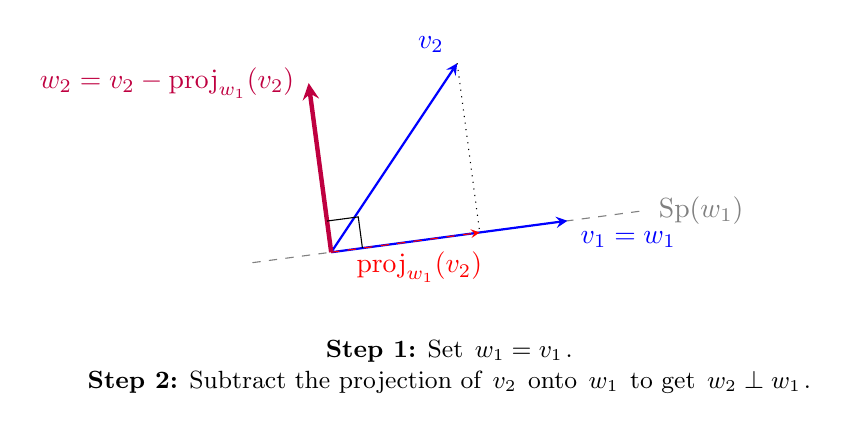
\begin{tikzpicture}[scale=2, >=stealth]
        % Coordinates
        \coordinate (O) at (0,0);
        \coordinate (V1) at (1.5, 0.2);
        \coordinate (V2) at (0.8, 1.2);
        
        % Subspace spanned by w1 (which is v1)
        \draw[dashed, gray] (-0.5, -0.066) -- (2, 0.266) node[right] {$\Sp(w_1)$};
        
        % Original vectors
        \draw[->, thick, blue] (O) -- (V1) node[below right] {$v_1 = w_1$};
        \draw[->, thick, blue] (O) -- (V2) node[above left] {$v_2$};
        
        % Projection of v2 onto w1
        \pgfmathsetmacro{\projcoeff}{((0.8*1.5 + 1.2*0.2)/(1.5*1.5 + 0.2*0.2))}
        \coordinate (Proj) at (\projcoeff*1.5, \projcoeff*0.2);
        \draw[->, dashed, red] (O) -- (Proj) node[pos=0.5, below, xshift=5pt] {$\operatorname{proj}_{w_1}(v_2)$};
        \draw[dotted] (V2) -- (Proj);
        
        % Resulting orthogonal vector w2
        \coordinate (W2) at (0.8-\projcoeff*1.5, 1.2-\projcoeff*0.2);
        \draw[->, ultra thick, purple] (O) -- (W2) node[left] {$w_2 = v_2 - \operatorname{proj}_{w_1}(v_2)$};
        
        % Right angle symbol
        \begin{scope}[rotate={atan2(0.2, 1.5)}]
            \draw (0.2, 0) -- (0.2, 0.2) -- (0, 0.2);
        \end{scope}

        \node[below, align=center, font=\small] at (0.75, -0.5) {
            \textbf{Step 1:} Set $w_1 = v_1$. \\
            \textbf{Step 2:} Subtract the projection of $v_2$ onto $w_1$ to get $w_2 \perp w_1$.
        };
    \end{tikzpicture}
\end{center}

\usetikzlibrary{calc}

\begin{figure}[h]
\centering
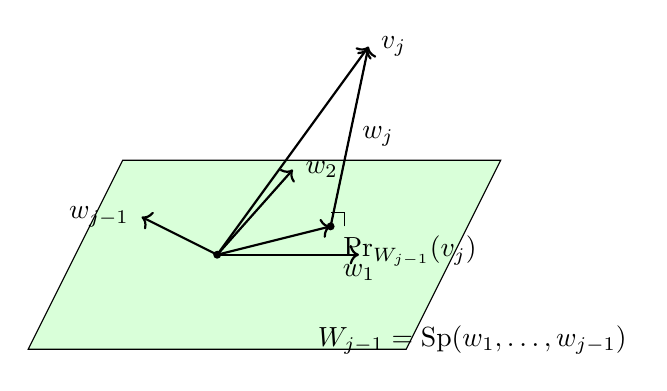
\begin{tikzpicture}[scale=1.2]

    % Plane W_{j-1}
    \fill[green!15] (-2,-1) -- (2,-1) -- (3,1) -- (-1,1) -- cycle;
    \draw (-2,-1) -- (2,-1) -- (3,1) -- (-1,1) -- cycle;
    \node at (2.7,-0.9) {$W_{j-1} = \Sp(w_1,\dots,w_{j-1})$};

    % Origin
    \coordinate (O) at (0,0);
    \fill (O) circle (1.2pt);

    % Basis vectors in the plane
    \coordinate (W1) at (1.5,0);
    \coordinate (W2) at (0.8,0.9);
    \coordinate (W3) at (-0.8,0.4);

    \draw[->, thick] (O) -- (W1);
    \node[below] at (W1) {$w_1$};

    \draw[->, thick] (O) -- (W2);
    \node[right] at (W2) {$w_2$};

    \draw[->, thick] (O) -- (W3);
    \node[left] at (W3) {$w_{j-1}$};

    % Projection point (in plane)
    \coordinate (P) at (1.2,0.3);
    \fill (P) circle (1.2pt);
    \node[below right] at (P) {$\Pr_{W_{j-1}}(v_j)$};

    % v_j vector (out of plane)
    \coordinate (V) at (1.6,2.2);
    \draw[->, thick] (O) -- (V);
    \node[right] at (V) {$v_j$};

    % w_j orthogonal component
    \draw[->, thick] (P) -- (V);
    \node[right] at ($(P)!0.5!(V)$) {$w_j$};

    % Projection vector
    \draw[->, thick] (O) -- (P);

    % Orthogonal drop
    \draw[dashed] (V) -- (P);

    % Right angle marker
    \draw ($(P)+(0.15,0)$) -- ($(P)+(0.15,0.15)$) -- ($(P)+(0,0.15)$);

\end{tikzpicture}
\caption{Geometric idea of Gram--Schmidt: the vectors $w_1,\dots,w_{j-1}$ span $W_{j-1}$, 
and $v_j$ decomposes as $v_j = w_j + \Pr_{W_{j-1}}(v_j)$ with $w_j \perp W_{j-1}$.}
\end{figure}

\usetikzlibrary{calc}

\begin{figure}[h]
\centering
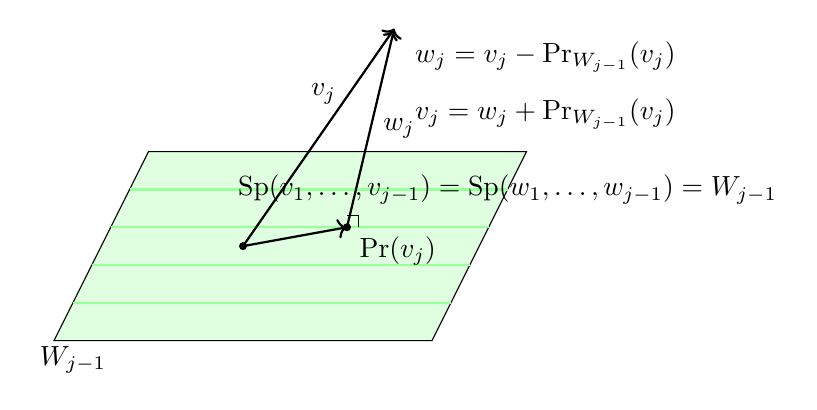
\begin{tikzpicture}[scale=1.2]

    % Plane W_{j-1}
    \fill[green!12] (-2,-1) -- (2,-1) -- (3,1) -- (-1,1) -- cycle;
    \draw (-2,-1) -- (2,-1) -- (3,1) -- (-1,1) -- cycle;

    % Light "hand-drawn" strokes
    \foreach \t in {0.2,0.4,0.6,0.8} {
        \draw[green!40, thick] 
            ($(-2,-1)!\t!(-1,1)$) -- ($(2,-1)!\t!(3,1)$);
    }

    % Label of plane
    \node at (-1.8,-1.2) {$W_{j-1}$};

    % Origin
    \coordinate (O) at (0,0);
    \fill (O) circle (1.2pt);

    % Projection point
    \coordinate (P) at (1.1,0.2);
    \fill (P) circle (1.2pt);
    \node[below right] at (P) {$\Pr(v_j)$};

    % v_j vector
    \coordinate (V) at (1.6,2.3);
    \draw[->, thick] (O) -- (V);
    \node[left] at ($(O)!0.7!(V)$) {$v_j$};

    % w_j vector
    \draw[->, thick] (P) -- (V);
    \node[right] at ($(P)!0.5!(V)$) {$w_j$};

    % projection vector
    \draw[->, thick] (O) -- (P);

    % dashed orthogonal drop
    \draw[dashed] (V) -- (P);

    % right angle marker
    \draw ($(P)+(0.12,0)$) -- ($(P)+(0.12,0.12)$) -- ($(P)+(0,0.12)$);

    % Span text
    \node at (2.8,0.6) 
    {$\Sp(v_1,\dots,v_{j-1})=\Sp(w_1,\dots,w_{j-1})=W_{j-1}$};

    % Formulas (like in sketch)
    \node at (3.2,2.0) 
    {$w_j = v_j - \Pr_{W_{j-1}}(v_j)$};

    \node at (3.2,1.4) 
    {$v_j = w_j + \Pr_{W_{j-1}}(v_j)$};

\end{tikzpicture}
\caption{Geometric idea behind the Gram--Schmidt process.}
\end{figure}


\begin{remark}
    In practice, the Gram-Schmidt process is often followed by a normalization step to produce an orthonormal basis. This two-stage process is essential for many numerical algorithms and theoretical results in linear algebra, such as the $QR$ decomposition.
\end{remark}
\input{content/euclidean-hermetian-spaces-b.tex}
\input{content/dual-spaces-inner-products-a.tex}
% \input{content/spectral-theorems.tex}
\setcounter{chapter}{23}
\renewcommand{\thetheorem}{24.a.\arabic{theorem}}
\setcounter{theorem}{0}

\chapter{Spectral Theorems}

\begin{ainote}
The professor left a note to \qt{explain the name} of the Spectral Theorems. In linear algebra, the \qt{spectrum} of a linear operator is its set of eigenvalues. The Spectral Theorems provide conditions under which an operator can be completely described by its spectrum—specifically, when there exists a basis for the entire space consisting solely of the operator's eigenvectors (making the operator diagonalizable).
\end{ainote}

% Def. (24.a.1)
\begin{definition}
\label{def:orthogonally_diagonalizable}
Let $V$ be an inner product space and $T \colon V \to V$ an endomorphism. We say that $T$ is \newterm{orthogonally diagonalizable} if there exists an orthonormal basis for $V$ consisting of eigenvectors of $T$.
\end{definition}

% Lemma. (24.a.2)
\begin{lemma}
\label{lem:orth_diag_implies_commute}
If $T$ is orthogonally diagonalizable, then $T \circ T^* = T^* \circ T$.
\end{lemma}

\begin{proof}
Let $\mathcal{B}$ be an orthonormal basis for $V$ such that all the vectors in $\mathcal{B}$ are eigenvectors of $T$. This implies that the representation matrix $[T]_{\mathcal{B}}^{\mathcal{B}}$ is a diagonal matrix. 

Since $\mathcal{B}$ is an orthonormal basis, we also know that the matrix of the adjoint map is the conjugate transpose of the matrix of the map, meaning $[T^*]_{\mathcal{B}}^{\mathcal{B}} = \left([T]_{\mathcal{B}}^{\mathcal{B}}\right)^*$. Since the conjugate transpose of a diagonal matrix is still a diagonal matrix, $[T^*]_{\mathcal{B}}^{\mathcal{B}}$ is also a diagonal matrix. 

If $M$ and $N$ are diagonal matrices, then they must commute, meaning $M \cdot N = N \cdot M$. Therefore, we have:
\[ [T]_{\mathcal{B}}^{\mathcal{B}} \cdot [T^*]_{\mathcal{B}}^{\mathcal{B}} = [T^*]_{\mathcal{B}}^{\mathcal{B}} \cdot [T]_{\mathcal{B}}^{\mathcal{B}}. \]
By the properties of representation matrices, this implies:
\[ [T \circ T^*]_{\mathcal{B}}^{\mathcal{B}} = [T^* \circ T]_{\mathcal{B}}^{\mathcal{B}} \implies T \circ T^* = T^* \circ T. \]
\end{proof}

% Def. (24.a.3)
\begin{definition}
\label{def:normal_endomorphism}
Let $V$ be an inner product space. An endomorphism $T \colon V \to V$ is called \newterm{normal} if $T \circ T^* = T^* \circ T$. 

Similarly, a matrix $A \in \M_{n \times n}(K)$ (where $K = \mathbb{R}$ or $\mathbb{C}$) is called \newterm{normal} if $A \cdot \overline{A}^\top = \overline{A}^\top \cdot A$. (Note that $A$ is a normal matrix if and only if the map $T_A \colon K^n \to K^n$ is a normal endomorphism, provided we endow $K^n$ with its standard inner product).
\end{definition}

We have seen in the previous lemma that if $T \colon V \to V$ is orthogonally diagonalizable, then $T$ is normal. 

\begin{question}
Is the converse statement true?
\end{question}

Over $K = \mathbb{R}$, the answer is NO! 
For example, consider the matrix $A = \left(\begin{smallmatrix} 0 & 1 \\ -1 & 0 \end{smallmatrix}\right)$. The linear map $T_A \colon \mathbb{R}^2 \to \mathbb{R}^2$ is a clockwise rotation by $90^\circ$, so there are no eigenvalues (in $\mathbb{R}$) and no eigenvectors. Thus, it cannot be diagonalizable. 
However, $\overline{A}^\top = A^\top = \left(\begin{smallmatrix} 0 & -1 \\ 1 & 0 \end{smallmatrix}\right)$, and we can easily check that $A \cdot A^\top = A^\top \cdot A = I_2$, meaning $A$ is indeed normal.

What about over $\mathbb{C}$?

% Thm. (24.a.4)
\begin{theorem}[Spectral Theorem over $\mathbb{C}$]
\label{thm:spectral_thm_c}
Let $V$ be a finite-di\-men\-sional inner product space over $\mathbb{C}$, and let $T \colon V \to V$ be a linear map. Then $T$ is orthogonally diagonalizable if and only if $T$ is normal.
\end{theorem}

For the proof, we need a lemma.

% Lemma. (24.a.5)
\begin{lemma}[Properties of Normal Endomorphisms]
\label{lem:properties_normal_endo}
Let $V$ be a finite-di\-men\-sional inner product space over $K$ (where $K = \mathbb{R}$ or $\mathbb{C}$). Let $T \colon V \to V$ be a normal endomorphism. Then:
\begin{enumerate}
    \item \textbf{(a)} For all $v \in V$, $\|Tv\| = \|T^*v\|$.
    \item \textbf{(b)} For all $\lambda \in K$, the endomorphism $T - \lambda \id_V$ is also normal.
    \item \textbf{(c)} If $v$ is an eigenvector of $T$ with eigenvalue $\lambda$, then $v$ is also an eigenvector of $T^*$ with eigenvalue $\overline{\lambda}$.
    \item \textbf{(d)} Let $v_1, v_2$ be eigenvectors of $T$ with eigenvalues $\lambda_1, \lambda_2$ respectively. If $\lambda_1 \neq \lambda_2$, then $\langle v_1, v_2 \rangle = 0$ (i.e., $v_1 \perp v_2$).
\end{enumerate}
\end{lemma}

\begin{proof}
\leavevmode
\begin{description}
    \item[Proof of (a):] We compute the squared norm:
    \[ \|Tv\|^2 = \langle Tv, Tv \rangle = \langle v, T^*Tv \rangle = \langle v, TT^*v \rangle = \langle T^*v, T^*v \rangle = \|T^*v\|^2, \]
    where we used the definition of the adjoint and the fact that $T$ is normal ($T \circ T^* = T^* \circ T$).
    
    \item[Proof of (b):] We expand the compositions:
    \begin{align*}
        (T - \lambda \id_V) \circ (T - \lambda \id_V)^* &= (T - \lambda \id_V) \circ (T^* - \overline{\lambda} \id_V) \\
        &= T \circ T^* - \overline{\lambda} T - \lambda T^* + \lambda \overline{\lambda} \id_V. \quad (*)
    \end{align*}
    On the other hand:
    \begin{align*}
        (T - \lambda \id_V)^* \circ (T - \lambda \id_V) &= (T^* - \overline{\lambda} \id_V) \circ (T - \lambda \id_V) \\
        &= T^* \circ T - \lambda T^* - \overline{\lambda} T + \overline{\lambda} \lambda \id_V. \quad (**)
    \end{align*}
    Because $T \circ T^* = T^* \circ T$, the expressions $(*)$ and $(**)$ are equal.
    
    \item[Proof of (c):] If $v$ is an eigenvector of $T$ with eigenvalue $\lambda$, then $(T - \lambda \id_V)v = 0$. By statement \textbf{(b)}, $T - \lambda \id_V$ is normal, hence by statement \textbf{(a)}, we have:
    \[ \|(T^* - \overline{\lambda} \id_V)v\| = \|(T - \lambda \id_V)v\| = \|0\| = 0. \]
    This implies that $(T^* - \overline{\lambda} \id_V)v = 0$, and therefore $T^*v = \overline{\lambda}v$.
    
    \item[Proof of (d):] We compute the inner product in two ways:
    \[ \lambda_1 \langle v_1, v_2 \rangle = \langle \lambda_1 v_1, v_2 \rangle = \langle Tv_1, v_2 \rangle = \langle v_1, T^*v_2 \rangle. \]
    By statement \textbf{(c)}, $T^*v_2 = \overline{\lambda_2}v_2$. Thus:
    \[ \langle v_1, T^*v_2 \rangle = \langle v_1, \overline{\lambda_2} v_2 \rangle = \lambda_2 \langle v_1, v_2 \rangle. \]
    Equating the two results gives $\lambda_1 \langle v_1, v_2 \rangle = \lambda_2 \langle v_1, v_2 \rangle$, which implies $(\lambda_1 - \lambda_2) \langle v_1, v_2 \rangle = 0$. 
    Since $\lambda_1 \neq \lambda_2$, we must have $\langle v_1, v_2 \rangle = 0$.
\end{description}
\end{proof}

\begin{proof}[Proof of the Spectral Theorem over $\mathbb{C}$ (\cref{thm:spectral_thm_c})]
We only need to prove the direction \qt{$T$ is normal $\implies T$ is orthogonally diagonalizable}, as the reverse direction was already established in \cref{lem:orth_diag_implies_commute}.

By a previous theorem, $T$ is trigonalizable (here we explicitly use the fact that $K = \mathbb{C}$ and the Fundamental Theorem of Algebra). That is, there exists a basis $\mathcal{C}$ for $V$ such that $[T]_{\mathcal{C}}^{\mathcal{C}}$ is an upper triangular matrix. 
By applying the Gram-Schmidt orthogonalization process to the basis $\mathcal{C}$, we obtain a new basis $\mathcal{B} = (v_1, \dots, v_n)$ which is orthonormal, and such that $[T]_{\mathcal{B}}^{\mathcal{B}}$ is still upper triangular. (This is left as an exercise to check. The main point is that if $\mathcal{C} = (u_1, \dots, u_n)$, then Gram-Schmidt gives an orthonormal basis $\mathcal{B} = (v_1, \dots, v_n)$ with $\Sp(v_1, \dots, v_k) = \Sp(u_1, \dots, u_k)$ for all $1 \leq k \leq n$).

We claim that $[T]_{\mathcal{B}}^{\mathcal{B}}$ is actually diagonal. To see this, let us write the matrix explicitly as $[T]_{\mathcal{B}}^{\mathcal{B}} = (a_{ij})_{1 \leq i \leq n, 1 \leq j \leq n}$:
\[ [T]_{\mathcal{B}}^{\mathcal{B}} = \begin{pmatrix} a_{11} & a_{12} & \dots & a_{1n} \\ 0 & a_{22} & \dots & a_{2n} \\ \vdots & \vdots & \ddots & \vdots \\ 0 & 0 & \dots & a_{nn} \end{pmatrix}. \]
Since $\mathcal{B}$ is orthonormal, the norm of $Tv_1$ is simply the norm of the first column of the matrix, which means $\|Tv_1\|^2 = |a_{11}|^2$. 
Since $[T^*]_{\mathcal{B}}^{\mathcal{B}} = \left([T]_{\mathcal{B}}^{\mathcal{B}}\right)^*$, the first column of $[T^*]_{\mathcal{B}}^{\mathcal{B}}$ is the conjugate transpose of the first row of $[T]_{\mathcal{B}}^{\mathcal{B}}$. Therefore, we also have:
\[ \|T^*v_1\|^2 = \sum_{k=1}^n |a_{1k}|^2 = |a_{11}|^2 + |a_{12}|^2 + \dots + |a_{1n}|^2. \]
As $T$ is normal, \cref{lem:properties_normal_endo} part \textbf{(a)} tells us that $\|Tv_1\| = \|T^*v_1\|$. This implies:
\[ |a_{11}|^2 = |a_{11}|^2 + |a_{12}|^2 + \dots + |a_{1n}|^2, \]
hence $a_{12} = \dots = a_{1n} = 0$. 
This shows that the matrix now looks like:
\[ [T]_{\mathcal{B}}^{\mathcal{B}} = \begin{pmatrix} a_{11} & 0 & \dots & 0 \\ 0 & a_{22} & \dots & a_{2n} \\ \vdots & 0 & \ddots & \vdots \\ 0 & 0 & \dots & a_{nn} \end{pmatrix}. \]
Now, consider $v_2$. We have $\|Tv_2\|^2 = |a_{22}|^2$ and $\|T^*v_2\|^2 = |a_{22}|^2 + |a_{23}|^2 + \dots + |a_{2n}|^2$. 
As $\|Tv_2\| = \|T^*v_2\|$, we similarly obtain $a_{23} = \dots = a_{2n} = 0$. 

We can continue this process by induction, and show that for all $1 \leq k < n$ we have $a_{k, k+1} = \dots = a_{k,n} = 0$. Hence, $[T]_{\mathcal{B}}^{\mathcal{B}}$ is diagonal. Since $\mathcal{B}$ is an orthonormal basis that diagonalizes $T$, it consists of eigenvectors, proving that $T$ is orthogonally diagonalizable.
\end{proof}

\begin{remark}
In the proof above, we used $K = \mathbb{C}$ \underline{only} at one place: when we stated that $T$ is trigonalizable. Therefore, we immediately obtain the following corollary for the real case.
\end{remark}

% Cor. (24.a.6)
\begin{corollary}
\label{cor:spectral_thm_real_trigonalizable}
Let $V$ be a finite-di\-men\-sional inner product space over $\mathbb{R}$, and $T \colon V \to V$ an endomorphism which is normal. If $T$ is trigonalizable (which is true if and only if the characteristic polynomial $P_T(x)$ factors as a product of linear factors over $\mathbb{R}$), then $T$ is orthogonally diagonalizable.
\end{corollary}

\subsection{The Spectral Theorem over \texorpdfstring{$\mathbb{R}$}{R}}

We've seen that over $\mathbb{R}$, the statement \qt{$T \in \End(V)$ is normal $\implies T$ is orthogonally diagonalizable} does not hold in general. We need a stronger condition.

% Lemma. (24.a.7)
\begin{lemma}
\label{lem:real_orth_diag_is_self_adj}
Let $V$ be a finite-di\-men\-sional inner product space over $\mathbb{R}$, and $T \in \End(V)$ which is orthogonally diagonalizable. Then $T^* = T$.
\end{lemma}

\begin{proof}
Let $\mathcal{B}$ be an orthonormal basis such that $[T]_{\mathcal{B}}^{\mathcal{B}}$ is a diagonal matrix. Since we are over $\mathbb{R}$, the conjugate transpose is simply the standard transpose. Then:
\[ [T^*]_{\mathcal{B}}^{\mathcal{B}} = \left([T]_{\mathcal{B}}^{\mathcal{B}}\right)^\top = [T]_{\mathcal{B}}^{\mathcal{B}}. \]
(The last equality holds because $[T]_{\mathcal{B}}^{\mathcal{B}}$ is diagonal). Because their representation matrices with respect to the same basis are equal, it follows that $T^* = T$.
\end{proof}

% Def. (24.a.8)
\begin{definition}
\label{def:self_adjoint}
Let $V$ be an inner product space over $K$ (where $K = \mathbb{R}$ or $\mathbb{C}$), and $T \in \End(V)$. $T$ is called \newterm{self adjoint} if $T^* = T$. 

Similarly, a matrix $A \in \M_{n \times n}(K)$ is called \newterm{self adjoint} if $A^* = A$. (Note that over $K = \mathbb{R}$, a self adjoint matrix is precisely a symmetric matrix, $A^\top = A$).
\end{definition}

\begin{exercise}
Show that $T \colon V \to V$ is self adjoint if and only if for every orthonormal basis $\mathcal{B}$ of $V$, the matrix $[T]_{\mathcal{B}}^{\mathcal{B}}$ is self adjoint.
\end{exercise}

% Thm. (24.a.9)
\begin{theorem}[Spectral Theorem over $\mathbb{R}$]
\label{thm:spectral_thm_r}
Let $V$ be a Euclidean space (i.e., an inner product space over $\mathbb{R}$) of finite dimension. Then $T$ is orthogonally diagonalizable if and only if $T$ is self adjoint.
\end{theorem}

For the proof, we need the following lemma:

% Lemma. (24.a.10)
\begin{lemma}
\label{lem:self_adj_properties}
Let $V$ be an inner product space over $K$ (where $K = \mathbb{R}$ or $\mathbb{C}$), and let $T \in \End(V)$ be self adjoint. Then:
\begin{enumerate}
    \item \textbf{(a)} All eigenvalues of $T$ are real.
    \item \textbf{(b)} The characteristic polynomial $P_T(x)$ factors into a product of linear factors over $K$.
\end{enumerate}
\end{lemma}

\begin{proof}
\leavevmode
\begin{description}
    \item[Proof of (a):] If $K = \mathbb{R}$, there is nothing to show. So assume $K = \mathbb{C}$. Let $\lambda \in \mathbb{C}$ be an eigenvalue and $v \in V$ a corresponding non-zero eigenvector. We've seen in \cref{lem:properties_normal_endo} \textbf{(c)} that $v$ is also an eigenvector of $T^*$ with eigenvalue $\overline{\lambda}$. But $T^* = T$. This implies:
    \[ \lambda v = Tv = T^*v = \overline{\lambda} v. \]
    Since $v \neq 0$, we must have $\lambda = \overline{\lambda}$, which implies $\lambda \in \mathbb{R}$.
    
    \item[Proof of (b):] For $K = \mathbb{C}$, this follows immediately from the Fundamental Theorem of Algebra. So assume $K = \mathbb{R}$. Let $\mathcal{B}$ be an orthonormal basis for $V$ and consider the matrix $A := [T]_{\mathcal{B}}^{\mathcal{B}} \in \M_{n \times n}(\mathbb{R})$. The statement would follow if we show that the characteristic polynomial $P_A(x)$ factors as a product of linear terms with real coefficients. 
    
    Now, $T^* = T$, hence $A = [T]_{\mathcal{B}}^{\mathcal{B}} = [T^*]_{\mathcal{B}}^{\mathcal{B}} = \left([T]_{\mathcal{B}}^{\mathcal{B}}\right)^* = A^* = A^\top$. 
    Consider $\mathbb{C}^n$ endowed with its standard inner product, and view $A$ as a matrix in $\M_{n \times n}(\mathbb{C})$. Let $T_A \colon \mathbb{C}^n \to \mathbb{C}^n$ be the corresponding linear map. The standard basis $\mathcal{E}_n = (e_1, \dots, e_n)$ is orthonormal, and $[T_A]_{\mathcal{E}_n}^{\mathcal{E}_n} = A$. 
    
    We know that $P_{T_A}(x) = P_A(x)$. When viewed as a polynomial over $\mathbb{C}$ (i.e., in $\mathbb{C}[x]$), it factors as a product of linear terms:
    \begin{equation}
        P_A(x) = \prod_{k=1}^n (x - \lambda_k) \in \mathbb{C}[x], \quad (*)
    \end{equation}
    where $\lambda_1, \dots, \lambda_n$ are the eigenvalues of $T_A$. But $T_A$ is self adjoint (even when viewed over $\mathbb{C}$ since $A^\top = A = A^*$), so by part \textbf{(a)}, all the eigenvalues $\lambda_1, \dots, \lambda_n \in \mathbb{R}$. Therefore, the factorization $(*)$ actually holds in $\mathbb{R}[x]$.
\end{description}
\end{proof}

\begin{proof}[Proof of the Spectral Theorem over $\mathbb{R}$ (\cref{thm:spectral_thm_r})]
The forward direction was proven in \cref{lem:real_orth_diag_is_self_adj}. For the reverse direction, if $T$ is self adjoint, then by \cref{lem:self_adj_properties}, its characteristic polynomial splits over $\mathbb{R}$. This implies $T$ is trigonalizable over $\mathbb{R}$. Furthermore, since $T = T^*$, $T$ trivially commutes with its adjoint, making it normal. By \cref{cor:spectral_thm_real_trigonalizable}, a normal map that is trigonalizable over $\mathbb{R}$ is orthogonally diagonalizable.
\end{proof}

\subsection{Spectral Theorems for Matrices}

Let $K = \mathbb{R}$ or $\mathbb{C}$. Recall that a matrix $A \in \M_{n \times n}(K)$ is called normal if $A \cdot A^* = A^* \cdot A$.

\begin{example}
\leavevmode
\begin{enumerate}
    \item For $K = \mathbb{R}$: Symmetric matrices and orthogonal matrices $\operatorname{O}(n)$ are normal.
    \item For $K = \mathbb{C}$: Self adjoint matrices and unitary matrices $\operatorname{U}(n)$ are normal.
\end{enumerate}
\end{example}

\begin{remark}
There exist symmetric matrices in $\M_{n \times n}(\mathbb{C})$ that are not normal. For example, let $A = \left(\begin{smallmatrix} i & i \\ i & 1 \end{smallmatrix}\right)$. We have $A^\top = A$, so it is symmetric. However, $A^* = \left(\begin{smallmatrix} -i & -i \\ -i & 1 \end{smallmatrix}\right)$. A quick calculation shows that $A \cdot A^* \neq A^* \cdot A$, so $A$ is not normal.
\end{remark}

% Thm. (24.a.11)
\begin{theorem}[Matrix Spectral Theorems]
\label{thm:spectral_thm_matrices}
\leavevmode
\begin{enumerate}[label=\textbf{(\alph*)}]
    \item If $A \in \M_{n \times n}(\mathbb{C})$ is normal, then there exists a unitary matrix $U \in \operatorname{U}(n)$ such that $U^{-1} A U$ is diagonal. (Note that $U^{-1} = U^*$).
    \item If $A \in \M_{n \times n}(\mathbb{R})$ is a symmetric matrix, then there exists an orthogonal matrix $O \in \operatorname{O}(n)$ such that $O^{-1} A O$ is diagonal. (Note that $O^{-1} = O^\top$).
\end{enumerate}
\end{theorem}

\begin{proof}[Proof Sketch]
The proof is left as an exercise, based on the following key points translating between maps and matrices:
\begin{enumerate}
    \item[(a)] $A \in \M_{n \times n}(\mathbb{C})$ is normal if and only if $T_A \colon \mathbb{C}^n \to \mathbb{C}^n$ is normal (when we endow $\mathbb{C}^n$ with its standard inner product).
    \item[(b)] If $\mathcal{B}$ is an orthonormal basis for $\mathbb{C}^n$, then the transition matrix $U := [\id_{\mathbb{C}^n}]_{\mathcal{E}_n}^{\mathcal{B}}$ is unitary.
    \item[(c)] $A \in \M_{n \times n}(\mathbb{R})$ is symmetric if and only if $T_A \colon \mathbb{R}^n \to \mathbb{R}^n$ is self adjoint, when we endow $\mathbb{R}^n$ with its standard inner product.
    \item[(d)] If $\mathcal{B}$ is an orthonormal basis for $\mathbb{R}^n$, then the transition matrix $O := [\id_{\mathbb{R}^n}]_{\mathcal{E}_n}^{\mathcal{B}}$ is orthogonal.
\end{enumerate}
\end{proof}

\section*{Exercise Solutions}
\addcontentsline{toc}{section}{Exercise Solutions}

\begin{exercisesolution}[Proof of Gram-Schmidt Preserving Upper Triangularity (on \cpageref{thm:spectral_thm_c})]~\\
Let $\mathcal{C} = (u_1, \dots, u_n)$ be a basis for $V$ such that the representation matrix $[T]_{\mathcal{C}}^{\mathcal{C}}$ is upper triangular. This means that for any $1 \leq k \leq n$, the vector $T(u_k)$ is a linear combination of $u_1, \dots, u_k$. In other words, $T(u_k) \in \Sp(u_1, \dots, u_k)$. Consequently, the subspace $W_k := \Sp(u_1, \dots, u_k)$ is $T$-invariant, meaning $T(W_k) \subseteq W_k$.

Applying the Gram-Schmidt orthogonalization process to the basis $\mathcal{C}$ produces an orthonormal basis $\mathcal{B} = (v_1, \dots, v_n)$ with the property that for every $1 \leq k \leq n$, the spans are preserved: $\Sp(v_1, \dots, v_k) = \Sp(u_1, \dots, u_k) = W_k$. 

Now, consider the matrix $[T]_{\mathcal{B}}^{\mathcal{B}}$. The $k$-th column of this matrix consists of the coordinates of $T(v_k)$ with respect to the basis $\mathcal{B}$. Since $v_k \in W_k$ and $W_k$ is $T$-invariant, we must have $T(v_k) \in W_k = \Sp(v_1, \dots, v_k)$. This means $T(v_k)$ can be written strictly as a linear combination of $v_1, \dots, v_k$, meaning all coefficients for vectors $v_j$ with $j > k$ are exactly zero. Therefore, $[T]_{\mathcal{B}}^{\mathcal{B}}$ is an upper triangular matrix.
\end{exercisesolution}

\begin{exercisesolution}[Proof of Matrix Self Adjointness Equivalence (on \cpageref{def:self_adjoint})] ~\\
Let $T \in \End(V)$.
First, suppose $T$ is self adjoint, so $T = T^*$. Let $\mathcal{B}$ be an arbitrary orthonormal basis for $V$. By the properties of representation matrices for adjoint maps in orthonormal bases, we have $[T^*]_{\mathcal{B}}^{\mathcal{B}} = \left([T]_{\mathcal{B}}^{\mathcal{B}}\right)^*$. Since $T = T^*$, we substitute to get $[T]_{\mathcal{B}}^{\mathcal{B}} = \left([T]_{\mathcal{B}}^{\mathcal{B}}\right)^*$, which means the matrix $[T]_{\mathcal{B}}^{\mathcal{B}}$ is self adjoint.

Conversely, suppose that for any orthonormal basis $\mathcal{B}$ of $V$, the matrix $[T]_{\mathcal{B}}^{\mathcal{B}}$ is self adjoint, i.e., $[T]_{\mathcal{B}}^{\mathcal{B}} = \left([T]_{\mathcal{B}}^{\mathcal{B}}\right)^*$. Again, using the identity $[T^*]_{\mathcal{B}}^{\mathcal{B}} = \left([T]_{\mathcal{B}}^{\mathcal{B}}\right)^*$, we see that $[T]_{\mathcal{B}}^{\mathcal{B}} = [T^*]_{\mathcal{B}}^{\mathcal{B}}$. Because the map sending an endomorphism to its representation matrix with respect to a fixed basis is an isomorphism, this equality of matrices implies the equality of the maps, hence $T = T^*$, meaning $T$ is self adjoint.
\end{exercisesolution}

\begin{exercisesolution}[Proof of \cref{thm:spectral_thm_matrices}]
\leavevmode
\begin{description}
    \item[Proof of (a):] Let $A \in \M_{n \times n}(\mathbb{C})$ be a normal matrix. By point (a), the linear map $T_A \colon \mathbb{C}^n \to \mathbb{C}^n$ is a normal endomorphism with respect to the standard inner product. By the Spectral Theorem over $\mathbb{C}$ (\cref{thm:spectral_thm_c}), $T_A$ is orthogonally diagonalizable. Thus, there exists an orthonormal basis $\mathcal{B} = (v_1, \dots, v_n)$ for $\mathbb{C}^n$ consisting of eigenvectors of $T_A$. 
    
    The representation matrix of $T_A$ with respect to $\mathcal{B}$, which is $[T_A]_{\mathcal{B}}^{\mathcal{B}}$, is a diagonal matrix $D$. Let $\mathcal{E}_n$ be the standard basis for $\mathbb{C}^n$. The transition matrix from $\mathcal{B}$ to $\mathcal{E}_n$ is $U := [\id_{\mathbb{C}^n}]_{\mathcal{E}_n}^{\mathcal{B}}$, whose columns are precisely the vectors $v_1, \dots, v_n$. Since $\mathcal{B}$ is an orthonormal basis, point (b) guarantees that $U$ is a unitary matrix. 
    
    Using the change of basis formula, we have:
    \[ D = [T_A]_{\mathcal{B}}^{\mathcal{B}} = [\id_{\mathbb{C}^n}]_{\mathcal{B}}^{\mathcal{E}_n} \cdot [T_A]_{\mathcal{E}_n}^{\mathcal{E}_n} \cdot [\id_{\mathbb{C}^n}]_{\mathcal{E}_n}^{\mathcal{B}} = U^{-1} \cdot A \cdot U. \]
    Thus, $U^{-1} A U$ is diagonal.
    
    \item[Proof of (b):] Let $A \in \M_{n \times n}(\mathbb{R})$ be a symmetric matrix. By point (c), the linear map $T_A \colon \mathbb{R}^n \to \mathbb{R}^n$ is self adjoint. By the Spectral Theorem over $\mathbb{R}$ (\cref{thm:spectral_thm_r}), $T_A$ is orthogonally diagonalizable. Thus, there exists an orthonormal basis $\mathcal{B}$ for $\mathbb{R}^n$ consisting of eigenvectors of $T_A$, making $[T_A]_{\mathcal{B}}^{\mathcal{B}}$ a diagonal matrix $D$. 
    
    Let $O := [\id_{\mathbb{R}^n}]_{\mathcal{E}_n}^{\mathcal{B}}$ be the transition matrix. Since $\mathcal{B}$ is an orthonormal basis in $\mathbb{R}^n$, point (d) guarantees that $O$ is an orthogonal matrix. 
    By the change of basis formula:
    \[ D = [T_A]_{\mathcal{B}}^{\mathcal{B}} = [\id_{\mathbb{R}^n}]_{\mathcal{B}}^{\mathcal{E}_n} \cdot [T_A]_{\mathcal{E}_n}^{\mathcal{E}_n} \cdot [\id_{\mathbb{R}^n}]_{\mathcal{E}_n}^{\mathcal{B}} = O^{-1} \cdot A \cdot O. \]
    Thus, $O^{-1} A O$ is diagonal.
\end{description}
\end{exercisesolution}
\renewcommand{\thetheorem}{25.a.\arabic{theorem}}
\setcounter{theorem}{0}
\setcounter{chapter}{24}

\chapter{Orthogonal and Unitary Maps / Isometries}

\section{Linear Isometries}

% Def. (25.a.1)
\begin{definition}[Linear Isometry]
\label{def:linear_isometry}
Let $V, W$ be inner product spaces over $K$ (where $K = \mathbb{R}$ or $\mathbb{C}$). A map $T \colon V \to W$ is called a \newterm{linear isometry} if $T$ is linear and for all $v_1, v_2 \in V$, 
\[ \langle Tv_1, Tv_2 \rangle_W = \langle v_1, v_2 \rangle_V. \]
(In other words, $T$ preserves the inner product).
\end{definition}

\begin{remark}
If $T \colon V \to W$ is a linear isometry, then:
\begin{enumerate}
    \item For all $v \in V$, $\|Tv\| = \|v\|$.
    \item For all $p, q \in V$, the distance is preserved:
    \[ \dist_W(Tp, Tq) = \|Tp - Tq\|_W = \|p - q\|_V = \dist_V(p, q). \]
    \item $T$ is injective. Indeed, if $v \in \ker T$, then $0 = \|Tv\| = \|v\|$, which implies $v = 0$. So, $\ker T = \{0\}$.
\end{enumerate}

\begin{center}
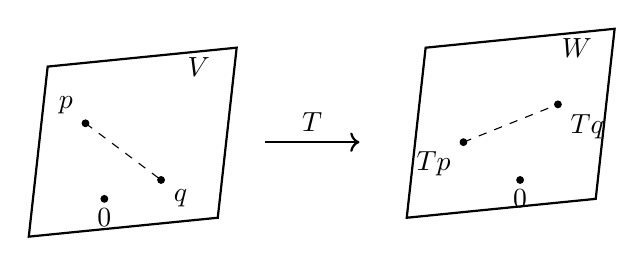
\begin{tikzpicture}[scale=1.2]
    % Space V
    \draw[thick] (0,0) -- (2,0.2) -- (2.2,2) -- (0.2,1.8) -- cycle;
    \node at (1.8, 1.8) {$V$};
    \filldraw (0.6, 1.2) circle (1pt) node[above left] {$p$};
    \filldraw (1.4, 0.6) circle (1pt) node[below right] {$q$};
    \draw[dashed] (0.6, 1.2) -- (1.4, 0.6);
    \filldraw (0.8, 0.4) circle (1pt) node[below] {$0$};

    % Arrow T
    \draw[->, thick] (2.5, 1) -- (3.5, 1) node[midway, above] {$T$};

    % Space W
    \draw[thick] (4,0.2) -- (6,0.4) -- (6.2,2.2) -- (4.2,2) -- cycle;
    \node at (5.8, 2.0) {$W$};
    \filldraw (4.6, 1.0) circle (1pt) node[below left] {$Tp$};
    \filldraw (5.6, 1.4) circle (1pt) node[below right] {$Tq$};
    \draw[dashed] (4.6, 1.0) -- (5.6, 1.4);
    \filldraw (5.2, 0.6) circle (1pt) node[below] {$0$};
\end{tikzpicture}
\end{center}
\end{remark}

From now on, we will concentrate on the case where $W = V$, meaning $T \in \End(V)$. If such a map $T$ is an isometry, we also call it an \newterm{orthogonal endomorphism} if $K = \mathbb{R}$, or a \newterm{unitary endomorphism} if $K = \mathbb{C}$.

% Thm. (25.a.2)
\begin{theorem}[Characterization of Isometries]
\label{thm:isometry_equivalences}
Let $V$ be a finite-di\-men\-sional inner product space over $\mathbb{R}$ or $\mathbb{C}$, and let $T \in \End(V)$. The following statements are equivalent:
\begin{enumerate}
    \item $T$ is an isometry.
    \item For all $v \in V$, $\|Tv\| = \|v\|$.
    \item For every orthonormal system $e_1, \dots, e_k$ of $V$, the list of vectors $Te_1, \dots, Te_k$ is also an orthonormal system.
    \item There exists an orthonormal \emph{basis} $\mathcal{B} := (e_1, \dots, e_n)$ of $V$ such that $Te_1, \dots, Te_n$ is also an orthonormal basis.
    \item $T \circ T^* = \id_V$.
    \item $T^* \circ T = \id_V$.
    \item $T^* = T^{-1}$.
    \item $T^*$ is an isometry.
\end{enumerate}
\end{theorem}

\begin{proof}
We will prove some of the equivalences here; the rest are left as exercises (and for the exercise sheet).

\textbf{(b)} $\implies$ \textbf{(a)}: Using the polarization identity (for the real case), we have:
\begin{align*}
    \langle Tv, Tw \rangle &= \frac{1}{2} \left( \|Tv + Tw\|^2 - \|Tv\|^2 - \|Tw\|^2 \right) \\
    &= \frac{1}{2} \left( \|T(v + w)\|^2 - \|Tv\|^2 - \|Tw\|^2 \right) \\
    &= \frac{1}{2} \left( \|v + w\|^2 - \|v\|^2 - \|w\|^2 \right) \\
    &= \langle v, w \rangle.
\end{align*}

\textbf{(a)} $\implies$ \textbf{(c)}: Let $e_1, \dots, e_k$ be an orthonormal system. Then, for all $1 \leq i, j \leq k$, we have:
\[ \langle Te_i, Te_j \rangle = \langle e_i, e_j \rangle = \delta_{ij}. \]
This implies that $Te_1, \dots, Te_k$ is also an orthonormal system.

\begin{ainote}
In the handwritten notes, the following proof is labeled as \textbf{(d)} $\implies$ \textbf{(e)}. However, it actually proves \textbf{(d)} $\implies$ \textbf{(f)}, which is $T^* \circ T = \id_V$. We have corrected the labeling here.
\end{ainote}

\textbf{(d)} $\implies$ \textbf{(f)}: Let $\mathcal{B} = (e_1, \dots, e_n)$ be an orthonormal basis such that $Te_1, \dots, Te_n$ is also an orthonormal system. Let $1 \leq j \leq n$. We have, for all $1 \leq i \leq n$:
\begin{equation}
    \langle e_i, e_j \rangle = \delta_{ij} = \langle Te_i, Te_j \rangle = \langle e_i, T^*Te_j \rangle. \quad (*)
\end{equation}
Since $(e_1, \dots, e_n)$ is a basis for $V$, the equality $(*)$ implies that by linearity in the first argument,
\[ \langle v, e_j \rangle = \langle v, T^*Te_j \rangle \quad \forall v \in V. \]
This implies that $T^*Te_j = e_j$. This last equality holds for all $1 \leq j \leq n$, which implies that $T^* \circ T = \id_V$.
\end{proof}

\section{Orthogonal and Unitary Matrices}

\noindent
Back to matrices. Recall that:
\begin{itemize}
    \item $A \in \M_{n \times n}(\mathbb{R})$ is orthogonal if $A\transp A = I \iff AA\transp = I \iff A^{-1} = A\transp$. The set of such matrices is $\Orth(n)$.
    \item $A \in \M_{n \times n}(\mathbb{C})$ is unitary if $A^* A = I \iff AA^* = I \iff A^{-1} = A^*$. The set of such matrices is $\Unit(n)$.
\end{itemize}

% Prop. (25.a.3)
\begin{proposition}
\label{prop:orth_unitary_matrix_rep}
Let $V$ be an $n$-di\-men\-sional inner product space over $\mathbb{R}$ (resp. $\mathbb{C}$). Let $\mathcal{B}$ be an orthonormal basis for $V$, and let $T \in \End(V)$. Then, $T$ is orthogonal (resp. unitary) if and only if $[T]_{\mathcal{B}}^{\mathcal{B}} \in \Orth(n)$ (resp. $[T]_{\mathcal{B}}^{\mathcal{B}} \in \Unit(n)$).
\end{proposition}

\begin{proof}
This is left as an exercise.
\end{proof}

Note that for all $A \in \Orth(n)$, we have $\det(A) = \pm 1$. Indeed:
\[ 1 = \det(I) = \det(AA\transp) = \det(A) \cdot \det(A\transp) = \det(A) \cdot \det(A) = \det(A)^2. \]

Similarly, for all $A \in \Unit(n)$, we have $|\det(A)| = 1$. Indeed:
\[ 1 = \det(AA^*) = \det(A) \cdot \det(\overline{A}\transp) = \det(A) \cdot \det(\overline{A}) = \det(A) \cdot \overline{\det(A)} = |\det(A)|^2. \]
(Note that $\det(A) \in \mathbb{C}$).

% Def. (25.a.4)
\begin{definition}[Special Orthogonal and Unitary Groups]
\label{def:special_groups}
We define the following subsets:
\begin{align*}
    \SOrth(n) &:= \{ A \in \Orth(n) \mid \det(A) = 1 \} \subseteq \Orth(n) \subseteq \GL_n(\mathbb{R}), \\
    \SUnit(n) &:= \{ A \in \Unit(n) \mid \det(A) = 1 \} \subseteq \Unit(n) \subseteq \GL_n(\mathbb{C}).
\end{align*}
\end{definition}

% Prop. (25.a.5)
\begin{proposition}[Group Properties]
\label{prop:group_properties}
Let $G$ be any of the sets $\Orth(n), \SOrth(n), \Unit(n)$, or $\SUnit(n)$. Then:
\begin{enumerate}
    \item $I_n \in G$.
    \item For all $A, B \in G$, $A \cdot B \in G$.
    \item For all $A \in G$, $A^{-1} \in G$.
\end{enumerate}
\end{proposition}

\begin{proof}
This is left as an exercise.
\end{proof}

\section{Classification of the Elements of O(2), O(3), etc.}

% Lemma. (25.a.6)
\begin{lemma}
\label{lem:eigenvalues_orthogonal}
Let $A \in \Orth(n)$. If $\lambda$ is a real eigenvalue of $A$, then $\lambda = \pm 1$.
\end{lemma}

\begin{proof}
Suppose $Av = \lambda v$, where $0 \neq v \in \mathbb{R}^n$. Then:
\[ \langle v, v \rangle = \langle Av, Av \rangle = \langle \lambda v, \lambda v \rangle = \lambda^2 \langle v, v \rangle. \]
As $v \neq 0$, we have $\langle v, v \rangle \neq 0$, which implies $\lambda^2 = 1$, and therefore $\lambda = \pm 1$.
\end{proof}

% Prop. (25.a.7)
\begin{proposition}[Classification of $\Orth(2)$]
\label{prop:classification_o2}
Let $A \in \Orth(2)$.
\begin{enumerate}
    \item If $\det A = 1$, then there exists $\theta \in [0, 2\pi)$ such that 
    \[ A = \begin{pmatrix} \cos\theta & -\sin\theta \\ \sin\theta & \cos\theta \end{pmatrix} := R_\theta. \]
    The map $T_A \colon \mathbb{R}^2 \to \mathbb{R}^2$ is an anti-clockwise rotation by an angle $\theta$.
    
    \item If $\det A = -1$, then there exists a basis $\mathcal{B} := (v_1, v_2)$ for $\mathbb{R}^2$ such that $T_A \colon \mathbb{R}^2 \to \mathbb{R}^2$ has the following representation matrix in the basis $\mathcal{B}$:
    \begin{equation}
        [T_A]_{\mathcal{B}}^{\mathcal{B}} = \begin{pmatrix} 1 & 0 \\ 0 & -1 \end{pmatrix}. \label{eq:reflection_matrix}
    \end{equation}
    In other words, $T_A$ performs a reflection with respect to the line $\ell := \Sp(v_1)$.
    Moreover, there exists $\theta \in [0, 2\pi)$ such that
    \[ A = \begin{pmatrix} \cos\theta & \sin\theta \\ \sin\theta & -\cos\theta \end{pmatrix} = R_\theta \cdot \begin{pmatrix} 1 & 0 \\ 0 & -1 \end{pmatrix}. \]
    The basis $\mathcal{B}$ for which \eqref{eq:reflection_matrix} holds is given by 
    \[ v_1 = \begin{pmatrix} \cos\left(\frac{\theta}{2}\right) \\ \sin\left(\frac{\theta}{2}\right) \end{pmatrix}, \quad v_2 = \begin{pmatrix} \cos\left(\frac{\theta}{2} + \frac{\pi}{2}\right) \\ \sin\left(\frac{\theta}{2} + \frac{\pi}{2}\right) \end{pmatrix}. \]
\end{enumerate}
\end{proposition}

\begin{center}
\begin{minipage}{0.45\textwidth}
\centering
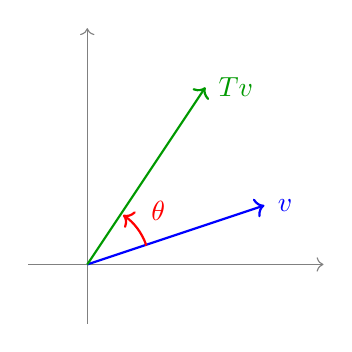
\begin{tikzpicture}[scale=1.5]
    \draw[->, gray] (-0.5, 0) -- (2, 0);
    \draw[->, gray] (0, -0.5) -- (0, 2);
    \draw[->, thick, blue] (0,0) -- (1.5, 0.5) node[right] {$v$};
    \draw[->, thick, green!60!black] (0,0) -- (1.0, 1.5) node[right] {$Tv$};
    \draw[->, red, thick] (0.5, 0.16) arc (18.4:56.3:0.5);
    \node[red] at (0.6, 0.45) {$\theta$};
\end{tikzpicture}
\end{minipage}
\begin{minipage}{0.45\textwidth}
\centering
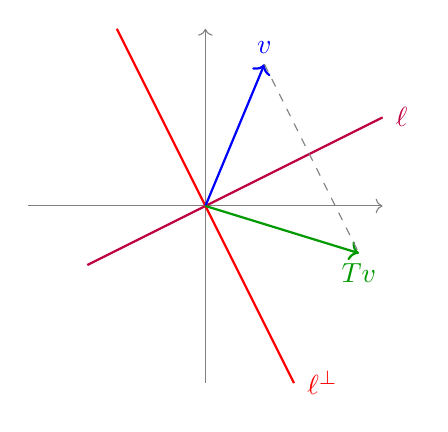
\begin{tikzpicture}[scale=1.5]
    \draw[->, gray] (-1.5, 0) -- (1.5, 0);
    \draw[->, gray] (0, -1.5) -- (0, 1.5);
    \draw[thick, purple] (-1, -0.5) -- (1.5, 0.75) node[right] {$\ell$};
    \draw[thick, red] (-0.75, 1.5) -- (0.75, -1.5) node[right] {$\ell^\perp$};
    \draw[->, thick, blue] (0,0) -- (0.5, 1.2) node[above] {$v$};
    \draw[->, thick, green!60!black] (0,0) -- (1.3, -0.4) node[below] {$Tv$};
    \draw[dashed, gray] (0.5, 1.2) -- (1.3, -0.4);
\end{tikzpicture}
\end{minipage}
\end{center}

\begin{proof}
Note that if $v \in \mathbb{R}^2$ has $\|v\| = 1$, then there exists $\theta \in [0, 2\pi)$ such that $v = \left(\begin{smallmatrix} \cos\theta \\ \sin\theta \end{smallmatrix}\right)$.

Now, let
\[
    A = \begin{pmatrix} | & | \\ u_1 & u_2 \\ | & | \end{pmatrix} \in \Orth(2).
\]
Since $A$ is orthogonal, its columns form an orthonormal basis. Thus, $\|u_1\| = 1$, which implies $u_1 = \left(\begin{smallmatrix} \cos\theta \\ \sin\theta \end{smallmatrix}\right)$ for some $\theta \in [0, 2\pi)$. 
We also have $u_1 \perp u_2$ and $\|u_2\| = 1$. 

The orthogonal complement to $u_1$ is:
\[ \begin{pmatrix} \cos\theta \\ \sin\theta \end{pmatrix}^\perp = \Sp \begin{pmatrix} \cos(\theta + \frac{\pi}{2}) \\ \sin(\theta + \frac{\pi}{2}) \end{pmatrix} = \Sp \begin{pmatrix} -\sin\theta \\ \cos\theta \end{pmatrix}. \]
Within the space $\Sp\left(\begin{smallmatrix} -\sin\theta \\ \cos\theta \end{smallmatrix}\right)$, there are precisely two elements with norm $1$, namely:
\[ u_2' = \begin{pmatrix} -\sin\theta \\ \cos\theta \end{pmatrix}, \quad u_2'' = \begin{pmatrix} \sin\theta \\ -\cos\theta \end{pmatrix}. \]

\begin{center}
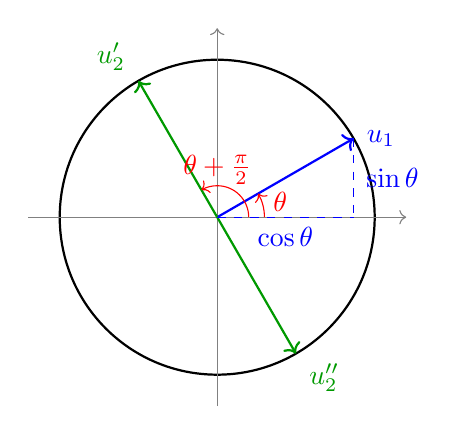
\begin{tikzpicture}[scale=2]
    \draw[thick] (0,0) circle (1cm);
    \draw[->, gray] (-1.2, 0) -- (1.2, 0);
    \draw[->, gray] (0, -1.2) -- (0, 1.2);
    
    \coordinate (U1) at (0.866, 0.5);
    \coordinate (U2P) at (-0.5, 0.866);
    \coordinate (U2PP) at (0.5, -0.866);
    
    \draw[->, thick, blue] (0,0) -- (U1) node[right] {$u_1$};
    \draw[->, thick, green!60!black] (0,0) -- (U2P) node[above left] {$u_2'$};
    \draw[->, thick, green!60!black] (0,0) -- (U2PP) node[below right] {$u_2''$};
    
    \draw[dashed, blue] (U1) -- (0.866, 0) node[midway, right] {$\sin\theta$};
    \draw[dashed, blue] (0,0) -- (0.866, 0) node[midway, below] {$\cos\theta$};
    
    \draw[->, red] (0.3, 0) arc (0:30:0.3);
    \node[red] at (0.4, 0.1) {$\theta$};
    
    \draw[->, red] (0.2, 0) arc (0:120:0.2);
    \node[red] at (0.0, 0.3) {$\theta + \frac{\pi}{2}$};
\end{tikzpicture}
\end{center}

If $u_2 = u_2'$, then $A = \left(\begin{smallmatrix} \cos\theta & -\sin\theta \\ \sin\theta & \cos\theta \end{smallmatrix}\right) = R_\theta$, and $\det A = 1$.

If $u_2 = u_2''$, then $A = \left(\begin{smallmatrix} \cos\theta & \sin\theta \\ \sin\theta & -\cos\theta \end{smallmatrix}\right) = R_\theta \cdot \left(\begin{smallmatrix} 1 & 0 \\ 0 & -1 \end{smallmatrix}\right)$, and $\det A = -1$.

In the second case, a direct calculation shows that $v_1 = \left(\begin{smallmatrix} \cos(\frac{\theta}{2}) \\ \sin(\frac{\theta}{2}) \end{smallmatrix}\right)$ and $v_2 = \left(\begin{smallmatrix} \cos(\frac{\theta}{2} + \frac{\pi}{2}) \\ \sin(\frac{\theta}{2} + \frac{\pi}{2}) \end{smallmatrix}\right)$ are eigenvectors of $A$ for the eigenvalues $\lambda_1 = 1$ and $\lambda_2 = -1$, respectively.
\end{proof}

\begin{summary}
$\SOrth(2) =$ rotations. \\
$\Orth(2) \setminus \SOrth(2) =$ reflections.
\end{summary}

% Cor. (25.a.8)
\begin{corollary}
\label{cor:2d_isometry_matrix}
Let $V$ be a 2-di\-men\-sional Euclidean space and $T \colon V \to V$ a linear isometry. Then $\det(T) = \pm 1$. 
Moreover, there exists an orthonormal basis $\mathcal{B}$ for $V$ such that:
\begin{enumerate}
    \item If $\det(T) = 1$, then $[T]_{\mathcal{B}}^{\mathcal{B}} = R_\theta$.
    \item If $\det(T) = -1$, then $[T]_{\mathcal{B}}^{\mathcal{B}} = \begin{pmatrix} 1 & 0 \\ 0 & -1 \end{pmatrix}$.
\end{enumerate}
\end{corollary}

% Prop. (25.a.9)
\begin{proposition}[Classification of $\SOrth(3)$]
\label{prop:classification_so3}
Let $A \in \SOrth(3)$. Then $1$ is an eigenvalue of $A$. 
Moreover, there exists an orthonormal basis $\mathcal{B} := (v_1, v_2, v_3)$ and $\theta \in [0, 2\pi)$ such that
\[ [T_A]_{\mathcal{B}}^{\mathcal{B}} = \begin{pmatrix} 1 & 0 & 0 \\ 0 & \cos\theta & -\sin\theta \\ 0 & \sin\theta & \cos\theta \end{pmatrix} = \begin{pmatrix} 1 & 0 \\ 0 & R_\theta \end{pmatrix}. \]
So, $T_A$ is a rotation with angle $\theta$ around the axis $\Sp(v_1)$. Moreover:
\begin{enumerate}
    \item If $-1$ is an eigenvalue of $A$, then $\theta = \pi$, hence
    \[ [T_A]_{\mathcal{B}}^{\mathcal{B}} = \begin{pmatrix} 1 & 0 & 0 \\ 0 & -1 & 0 \\ 0 & 0 & -1 \end{pmatrix}. \]
    \item If $-1$ is \emph{not} an eigenvalue of $A$ (which is true if and only if $1$ is the only real eigenvalue), then $\theta \neq \pi$.
\end{enumerate}
\end{proposition}

\begin{center}
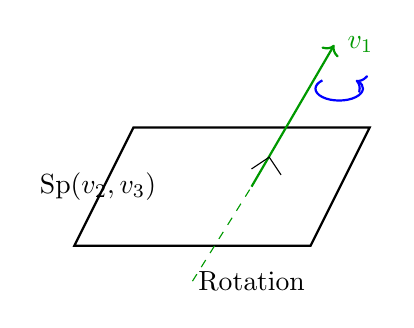
\begin{tikzpicture}[scale=1.5]
    % Plane
    \draw[thick] (-1,-0.5) -- (1,-0.5) -- (1.5, 0.5) -- (-0.5, 0.5) -- cycle;
    \node at (-0.8, 0) {$\Sp(v_2, v_3)$};
    
    % Axis v1
    \draw[->, thick, green!60!black] (0.5, 0) -- (1.2, 1.2) node[right] {$v_1$};
    \draw[dashed, green!60!black] (0, -0.8) -- (0.5, 0);
    
    % Right angle
    \draw (0.5, 0.15) -- (0.65, 0.25) -- (0.75, 0.1);
    
    % Rotation arrow
    \draw[->, thick, blue] (1.1, 0.9) arc (135:405:0.2 and 0.1);
    \node at (0.5, -0.8) {Rotation};
\end{tikzpicture}
\end{center}

\begin{proof}
The characteristic polynomial $P_A(x)$ of $A$ is a polynomial of degree $3$ with real coefficients. By the Intermediate Value Theorem from analysis, any odd-degree polynomial with real coefficients has at least one real zero $\lambda \in \mathbb{R}$ of $P_A(x)$ (i.e., $P_A(\lambda) = 0$). This implies that $A$ has at least one real eigenvalue. 
By a previous theorem (\ref{lem:eigenvalues_orthogonal}), $\lambda = \pm 1$.

Let $v_1 \in \mathbb{R}^3$ be an eigenvector of $\lambda$. By normalizing it if necessary, we may assume $\|v_1\| = 1$. Consider the subspace
\[ L := v_1^\perp = \{v \in \mathbb{R}^3 \mid v \perp v_1\}. \]
Since $A$ is orthogonal, we have for all $v \in L$, $A \cdot v \in L$. (i.e., $T_A(L) \subseteq L$, meaning $L$ is invariant under $T_A$).
Indeed, if $v \in L$, this implies $0 = \langle v, v_1 \rangle$. Because $A \in \Orth(3)$, it preserves inner products:
\[ 0 = \langle v, v_1 \rangle = \langle Av, Av_1 \rangle = \langle Av, \pm v_1 \rangle = \pm \langle Av, v_1 \rangle \implies Av \in L. \]

We also have $\mathbb{R}^3 = \Sp(v_1) \oplus L$, hence $\dim L = 2$.
Now, $T_A|_L \colon L \to L$ is a linear isometry. Let $\mathcal{L} = (w_1, w_2)$ be an orthonormal basis for $L$. By a previous result, the representation matrix is $Q := [T_A|_L]_{\mathcal{L}}^{\mathcal{L}} \in \Orth(2)$.

\textbf{Case (a):} $\lambda = 1$. Take the basis $\mathcal{B} := (v_1, w_1, w_2)$. Then
\[ [T_A]_{\mathcal{B}}^{\mathcal{B}} = \begin{pmatrix} 1 & 0 & 0 \\ 0 & \multicolumn{2}{c}{\multirow{2}{*}{$Q$}} \\ 0 & & \end{pmatrix} = \begin{pmatrix} 1 & 0 \\ 0 & Q \end{pmatrix}. \]
Now, $1 = \det A = \det(T_A) = 1 \cdot \det(Q)$, which implies $\det Q = 1$. 
So, $Q \in \SOrth(2)$. By the previous proposition (\ref{prop:classification_o2}), there exists $\theta \in [0, 2\pi)$ such that $Q = R_\theta$.
Thus,
\[ [T_A]_{\mathcal{B}}^{\mathcal{B}} = \begin{pmatrix} 1 & 0 \\ 0 & R_\theta \end{pmatrix}. \]

\textbf{Case (b):} If $\lambda = -1$. By the same argument as for case (a), we get that $1 = \det A = (-1) \cdot \det(T_A|_L)$, which implies $\det(T_A|_L) = -1$. By \cref{cor:2d_isometry_matrix}, there exists an orthonormal basis $\mathcal{L} = (w_1, w_2)$ for $L$ such that $[T_A|_L]_{\mathcal{L}}^{\mathcal{L}} = \left(\begin{smallmatrix} 1 & 0 \\ 0 & -1 \end{smallmatrix}\right)$.
Take $\mathcal{B}' := (v_1, w_1, w_2)$. Then
\[ [T_A]_{\mathcal{B}'}^{\mathcal{B}'} = \begin{pmatrix} -1 & 0 & 0 \\ 0 & 1 & 0 \\ 0 & 0 & -1 \end{pmatrix}. \]
And for the reordered basis $\mathcal{B} := (w_1, v_1, w_2)$, we have 
\[ [T_A]_{\mathcal{B}}^{\mathcal{B}} = \begin{pmatrix} 1 & 0 & 0 \\ 0 & -1 & 0 \\ 0 & 0 & -1 \end{pmatrix} = \begin{pmatrix} 1 & 0 \\ 0 & R_\pi \end{pmatrix}. \]
Note that in case \textbf{(b)} too, $1$ is an eigenvalue of $A$ (corresponding to the eigenvector $w_1$).
\end{proof}

% Prop. (25.a.10)
\begin{proposition}[Classification of $\Orth(3) \setminus \SOrth(3)$]
\label{prop:classification_o3_minus_so3}
Let $A \in \Orth(3) \setminus \SOrth(3)$. Then there exists an orthonormal basis $\mathcal{B} := (v_1, v_2, v_3)$ for $\mathbb{R}^3$ such that 
\[ [T_A]_{\mathcal{B}}^{\mathcal{B}} = \begin{pmatrix} -1 & 0 & 0 \\ 0 & \cos\theta & -\sin\theta \\ 0 & \sin\theta & \cos\theta \end{pmatrix} = \begin{pmatrix} -1 & 0 \\ 0 & R_\theta \end{pmatrix} \]
for some $\theta \in [0, 2\pi)$. (So $T_A$ does a rotation by $\theta$ around $\Sp(v_1)$, followed by a reflection with respect to $\Sp(v_2, v_3)$).
\end{proposition}

\begin{proof}
Let $A' := -A = (-I) \cdot A$. Then $A' \in \Orth(3)$ and $\det A' = (-1)^3 \cdot \det A = (-1) \cdot (-1) = 1$.
This implies $A' \in \SOrth(3)$. By the previous proposition (\ref{prop:classification_so3}), there exists an orthonormal basis $\mathcal{B}$ for $\mathbb{R}^3$, and $\theta' \in [0, 2\pi)$, such that $[T_{A'}]_{\mathcal{B}}^{\mathcal{B}} = \left(\begin{smallmatrix} 1 & 0 \\ 0 & R_{\theta'} \end{smallmatrix}\right)$. 
This implies:
\begin{align*}
    [T_A]_{\mathcal{B}}^{\mathcal{B}} &= [-\id_{\mathbb{R}^3}]_{\mathcal{B}}^{\mathcal{B}} \cdot [T_{A'}]_{\mathcal{B}}^{\mathcal{B}} \\
    &= -I \cdot \begin{pmatrix} 1 & 0 \\ 0 & R_{\theta'} \end{pmatrix} \\
    &= \begin{pmatrix} -1 & 0 \\ 0 & -R_{\theta'} \end{pmatrix} \\
    &= \begin{pmatrix} -1 & 0 \\ 0 & R_\theta \end{pmatrix},
\end{align*}
where $\theta = (\theta' + \pi) \pmod{2\pi}$. 
(Note that $-R_{\theta'} = R_\pi \circ R_{\theta'} = R_{\theta' + \pi}$).
\end{proof}


\section*{Exercise Solutions}
\addcontentsline{toc}{section}{Exercise Solutions}

\begin{exercisesolution}[Proof of \cref{thm:isometry_equivalences} \textbf{(d)} $\implies$ \textbf{(e)}]
Assume there exists an orthonormal basis $\mathcal{B} = (e_1, \dots, e_n)$ of $V$ such that $Te_1, \dots, Te_n$ is also an orthonormal basis. Since it is an orthonormal basis, we have $\langle Te_i, Te_j \rangle = \delta_{ij}$. 
By the definition of the adjoint map, we can rewrite the inner product as:
\[ \delta_{ij} = \langle Te_i, Te_j \rangle = \langle e_i, T^*Te_j \rangle. \]
Because the vectors $e_i$ form a basis, the fact that the inner product of $T^*Te_j$ with every basis vector $e_i$ yields $\delta_{ij}$ (which are precisely the coordinates of $e_j$) implies that $T^*Te_j = e_j$ for all $1 \leq j \leq n$.
Since the linear map $T^* \circ T$ acts as the identity on a basis, it must be the identity map on the entire space $V$. Thus, $T^* \circ T = \id_V$. (This proves \textbf{(d)} $\implies$ \textbf{(f)}).
Since $V$ is finite-di\-men\-sional, a left inverse is also a right inverse, so $T \circ T^* = \id_V$, proving \textbf{(e)}.
\end{exercisesolution}

\begin{exercisesolution}[Proof of \cref{prop:orth_unitary_matrix_rep}]
Let $\mathcal{B} = (e_1, \dots, e_n)$ be an orthonormal basis for $V$. 
First, suppose $T$ is an orthogonal (resp. unitary) endomorphism. By \cref{thm:isometry_equivalences}, $T \circ T^* = \id_V$ and $T^* \circ T = \id_V$. 
Taking the representation matrix with respect to $\mathcal{B}$, we have:
\[ [T^* \circ T]_{\mathcal{B}}^{\mathcal{B}} = [\id_V]_{\mathcal{B}}^{\mathcal{B}} = I_n. \]
By the properties of representation matrices, this splits into $[T^*]_{\mathcal{B}}^{\mathcal{B}} \cdot [T]_{\mathcal{B}}^{\mathcal{B}} = I_n$. Since $\mathcal{B}$ is an orthonormal basis, $[T^*]_{\mathcal{B}}^{\mathcal{B}} = \left([T]_{\mathcal{B}}^{\mathcal{B}}\right)^*$. 
Thus, $\left([T]_{\mathcal{B}}^{\mathcal{B}}\right)^* \cdot [T]_{\mathcal{B}}^{\mathcal{B}} = I_n$, which means the matrix $[T]_{\mathcal{B}}^{\mathcal{B}}$ is orthogonal (resp. unitary).

Conversely, assume that $A := [T]_{\mathcal{B}}^{\mathcal{B}}$ is orthogonal (resp. unitary). This means $A^* A = I_n$. 
Because $\mathcal{B}$ is an orthonormal basis, $A^* = \left([T]_{\mathcal{B}}^{\mathcal{B}}\right)^* = [T^*]_{\mathcal{B}}^{\mathcal{B}}$. 
Substituting this back yields $[T^*]_{\mathcal{B}}^{\mathcal{B}} \cdot [T]_{\mathcal{B}}^{\mathcal{B}} = I_n$, and therefore $[T^* \circ T]_{\mathcal{B}}^{\mathcal{B}} = [\id_V]_{\mathcal{B}}^{\mathcal{B}}$. This implies the maps are equal, so $T^* \circ T = \id_V$. By \cref{thm:isometry_equivalences}, this guarantees $T$ is an isometry.
\end{exercisesolution}

\begin{exercisesolution}[Proof of \cref{prop:group_properties}]
We will prove this generically for $G = \Unit(n)$ and $G = \SUnit(n)$ (the real cases are identical, replacing the conjugate transpose $^*$ with the transpose $\transp$).
\begin{enumerate}[label=\textbf{(\alph*)}]
    \item The identity matrix $I_n$ satisfies $I_n^* \cdot I_n = I_n \cdot I_n = I_n$, so $I_n \in \Unit(n)$. Furthermore, $\det(I_n) = 1$, so $I_n \in \SUnit(n)$.
    
    \item Let $A, B \in \Unit(n)$. We evaluate $(AB)^* (AB) = (B^* A^*) (AB) = B^* (A^* A) B$. Since $A \in \Unit(n)$, $A^* A = I_n$, so this reduces to $B^* I_n B = B^* B$. Since $B \in \Unit(n)$, $B^* B = I_n$. Thus, $AB \in \Unit(n)$. 
    If additionally $A, B \in \SUnit(n)$, then $\det(AB) = \det(A)\det(B) = 1 \cdot 1 = 1$, so $AB \in \SUnit(n)$.
    
    \item Let $A \in \Unit(n)$. This implies $A^* A = I_n$, meaning $A^{-1} = A^*$. We check if $A^{-1}$ is unitary: $(A^{-1})^* A^{-1} = (A^*)^* A^* = A A^* = I_n$. Thus, $A^{-1} \in \Unit(n)$. 
    If additionally $A \in \SUnit(n)$, then $\det(A^{-1}) = \frac{1}{\det(A)} = \frac{1}{1} = 1$, so $A^{-1} \in \SUnit(n)$.
\end{enumerate}
\end{exercisesolution}
\end{document}
